\documentclass[leqno,b5paper]{book}


\usepackage{khalidUrduBooksEMT}                     %my sty file
%\usepackage{animate}

\sisetup{math-micro=\text{µ},text-micro=µ}           %siunitx stopped showing micro symbol and had to put this line. now the size of micro is smaller


%this file describes urdu commands for the commonly used english latex commands

%chapter, section etc
\newcommand*{\باب}[1]{\chapter{#1}}                                      %defining commonly used commands
\newcommand*{\حصہ}[1]{\section{#1}}
\newcommand*{\جزوحصہ}[1]{\subsection{#1}}
\newcommand*{\جزوجزوحصہ}[1]{\subsubsection{#1}}

\newcommand*{\بابء}[1]{\chapter*{#1}}                                      %defining commonly used commands
\newcommand*{\حصہء}[1]{\section*{#1}}
\newcommand*{\جزوحصہء}[1]{\subsection*{#1}}
\newcommand*{\جزوجزوحصہء}[1]{\subsubsection*{#1}}


%english text in urdu mode
\newcommand*{\تحریر}[1]{\textenglish{#1}}	% english text in urduMode
\newcommand*{\موٹا}[1]{\textbf{#1}}
\newcommand*{\ترچہ}[1]{{\textit{#1}}}
\newcommand*{\اصطلاح}[1]{{\textbf{#1}}}

%end commands cannot be redefined and as such these two are not usable
\providecommand*{\ابتدا}[1]{\begin{#1}}
\providecommand*{\انتہا}[1]{\end{#1}}

%include and input directives for adding external files into the main document 
\newcommand*{\بشمول}[1]{\includeonly{#1}}
\newcommand*{\شامل}[1]{\include{#1}}
\newcommand*{\داخل}[1]{\input{#1}}

%to use extra latex packages
\newcommand*{\استعمال}[1]{\usepackage{#1}}

%footnotes and indexes
\newcommand*{\حاشیہب}[1]{{\raggedright{\footnote{\textenglish{#1}}}} }               %footnote to the left hand side
\newcommand*{\حاشیہد}[1]{{\raggedleft{\footnote{#1}}}}
\newcommand*{\حاشیہط}[1]{\marginpar{#1}}

\newcommand*{\فرہنگ}[1]{\index{#1}}

%references and labels
\newcommand*{\شناخت}[1]{\label{#1}}
\newcommand*{\حوالہ}[1]{\ref{#1}}
\newcommand*{\حوالہصفحہ}[1]{\pageref{#1}}

%counters
\newcommand*{\فاصلہ}{\vspace*{10mm}}

%itemize, bullets and numbered items   
\newcommand*{\اشیاء}{itemize}                               %used in   \begin{itemize}
\newcommand*{\شے}[1]{\item {#1}}			%used in    \item
%description
\newcommand*{\جزو}[1]{\item[#1]}
%maths commands
\newcommand*{\عددی}[1]{\: \ensuremath{#1} \:} % in-line math & inside math mode
\newcommand*{\عددیء}[1]{\ensuremath{#1}}
\newcommand*{\سمتیہ}[1]{\ensuremath{{\bf{#1}}}}
\newcommand*{\سمتیازیرنوشت}[2]{\ensuremath{{\boldsymbol{#1}}_{\textup{#2}}}}

\newcommand*{\ضرب}{\time}					%multiplication symbol
\newcommand*{\نکطہد}{\cdot}
\newcommand*{\نقطے}{\ensuremath{\cdots}}

\newcommand*{\زیرنوشت}[3]{\: \ensuremath{{#1_{#2 \textrm {#3}}}} \:}   %english+urdu subscript \زیرنوشت{V}{CE}{غیرافزائندہ}
\newcommand*{\سیدھازیرنوشت}[2]{\: \ensuremath{{#1_{\textup{#2}}}} \:} %RC

\newcommand*{\قریب}[1]{\mbox{#1}}

\renewcommand{\indexname}{فرہنگ}        %apparently did nothing
%===============================


%numbering scheme
\renewcommand*{\thefigure}{\arabic{figure}.\thechapter}
\renewcommand*{\thetable}{\arabic{table}.\thechapter}
\renewcommand*{\theequation}{\arabic{equation}.\thechapter}
\renewcommand*{\thesection}{\arabic{section}.\thechapter}
\renewcommand*{\thesubsection}{\arabic{subsection}.\arabic{section}.\thechapter}
\renewcommand*{\thesubsubsection}{\arabic{subsubsection}.\arabic{subsection}.\arabic{section}.\thechapter}

%================
%my environments
%================

%environment for examples مثال
\newcounter{examplecounter}[chapter]
\renewcommand{\theexamplecounter}{\arabic{examplecounter}.\thechapter}

\newenvironment*{مثال}
{\noindent\ignorespaces \vspace{\baselineskip} \hrule \vspace{\baselineskip}  مثال \refstepcounter{examplecounter} \theexamplecounter :}%
{\par\noindent \hrule  \vspace{\baselineskip}}

%------
%practice problems environment مشق

\newcounter{practicecounter}[chapter]                              %practice here means مشق
\renewcommand{\thepracticecounter}{\arabic{practicecounter}.\thechapter}

\newenvironment*{مشق}
{\noindent\ignorespaces \vspace{\baselineskip} \hrule \vspace{\baselineskip} مشق \refstepcounter{practicecounter} \thepracticecounter :}%
{\par\noindent \hrule  \vspace{\baselineskip}}
%---------

%end of chapter questions environment سوال

\newcounter{questioncounter}[chapter]
\renewcommand{\thequestioncounter}{\arabic{questioncounter}.\thechapter}

\newenvironment*{سوال}				
{\noindent\ignorespaces  سوال \refstepcounter{questioncounter} \thequestioncounter :}%
{\par\noindent }
%--------------------

%defining a LAW   قانون

\newcounter{lawcounter}[chapter]
\renewcommand{\thelawcounter}{\arabic{lawcounter}.\thechapter}

\newenvironment*{قانون}				
{\par\medskip \refstepcounter{lawcounter} }%
{\par\medskip }
%--------------------

                  %turning latex into urdu
% Greek Letters for Urdu Latex usage

\newcommand*{\ایلفا}{\alpha}
\newcommand*{\بیٹا}{\beta}
\newcommand*{\گیما}{\gamma}
\newcommand*{\ڈیلٹا}{\delta}
\newcommand*{\ایپسلان}{\epsilon}
\newcommand*{\متغیرایپسلان}{\varepsilon}
\newcommand*{\زیٹا}{\zeta}
\newcommand*{\ایٹا}{\eta}
\newcommand*{\تھیٹا}{\theta}
\newcommand*{\متغیرتھیٹا}{\vartheta}
\newcommand*{\ایوٹا}{\iota}
\newcommand*{\کاپا}{\kappa}
\newcommand*{\لیمڈا}{\lambda}
\newcommand*{\میو}{\mu}
\newcommand*{\نیو}{\nu}
\newcommand*{\ژاے}{\xi}
\newcommand*{\پاے}{\pi}
\newcommand*{\متغیرپاے}{\varpi}
\newcommand*{\رھو}{\rho}
\newcommand*{\متغیررھو}{\varrho}
\newcommand*{\سگما}{\sigma}
\newcommand*{\متغیرسگما}{\varsigma}
\newcommand*{\ٹو}{\tau}
\newcommand*{\اپسیلان}{\upsilon}
\newcommand*{\فاے}{\phi}
\newcommand*{\متغیفاے}{\varphi}
\newcommand*{\چاے}{\chi}
\newcommand*{\ساے}{\psi}
\newcommand*{\اومیگا}{\omega}

\newcommand*{\بڑاگیما}{\Gamma}
\newcommand*{\بڑاڈیلٹا}{\Delta}
\newcommand*{\بڑاتھیٹا}{\Theta}
\newcommand*{\بڑالیمڈا}{\Lambda}
\newcommand*{\بڑاژاے}{\Xi}
\newcommand*{\بڑاپاے}{\Pi}
\newcommand*{\بڑاسگما}{\Sigma}
\newcommand*{\بڑاساے}{\Psi}
\newcommand*{\بڑااومیگا}{\Omega}



\newcommand*{\kvec}[1]{{\ensuremath{{\boldsymbol{#1}}}}}
\newcommand*{\kvecsub}[2]{{\ensuremath{{\boldsymbol{#1}}}_{\textup{#2}}}}

\newcommand*{\ax}{\ensuremath{{\boldsymbol{a}}_{\textup{x}}}}
\newcommand*{\ay}{\ensuremath{{\boldsymbol{a}}_{\textup{y}}}}
\newcommand*{\az}{\ensuremath{{\boldsymbol{a}}_{\textup{z}}}}
%
\newcommand*{\arho}{\ensuremath{{\boldsymbol{a}}_{\rho}}}
\newcommand*{\aphi}{\ensuremath{{\boldsymbol{a}}_{\phi}}}
%
\newcommand*{\ar}{\ensuremath{{\boldsymbol{a}}_{\textup{r}}}}
\newcommand*{\atheta}{\ensuremath{{\boldsymbol{a}}_{\theta}}}

\newcommand*{\aN}{\ensuremath{{\boldsymbol{a}}_N}}
\newcommand*{\aR}{\ensuremath{{\boldsymbol{a}}_{\textup{R}}}}

\newcommand*{\au}{\ensuremath{{\boldsymbol{a}}_u}}
\newcommand*{\av}{\ensuremath{{\boldsymbol{a}}_v}}
\newcommand*{\aw}{\ensuremath{{\boldsymbol{a}}_w}}

\newcommand*{\Ex}{\ensuremath{{\boldsymbol{E}}_x}}
\newcommand*{\Ey}{\ensuremath{{\boldsymbol{E}}_y}}
\newcommand*{\Ez}{\ensuremath{{\boldsymbol{E}}_z}}
%
\newcommand*{\Erho}{\ensuremath{{\boldsymbol{E}}_{\rho}}}
\newcommand*{\Ephi}{\ensuremath{{\boldsymbol{E}}_{\phi}}}
%
\newcommand*{\Er}{\ensuremath{{\boldsymbol{E}}_r}}
\newcommand*{\Etheta}{\ensuremath{{\boldsymbol{E}}_{\theta}}}
%===========================
\newcommand{\RightAngle}[4][5pt]{%
        \draw[gray] ($#3!#1!#2$)
        --($ #3!2!($($#3!#1!#2$)!.5!($#3!#1!#4$)$) $)
        --($#3!#1!#4$) ;        }

%%still decided to format everything at the very end
%try to make a jump table so that a single command can be built

\newcommand*{\ksubRB}{\ensuremath{R_{\textup{B}}}}   %transistor
\newcommand*{\ksubRC}{\ensuremath{R_{\textup{C}}}}
\newcommand*{\ksubRE}{\ensuremath{R_{\textup{E}}}}

\newcommand*{\ksubRG}{\ensuremath{R_{\textup{G}}}}	%mosfet
\newcommand*{\ksubRD}{\ensuremath{R_{\textup{D}}}}
\newcommand*{\ksubRS}{\ensuremath{R_{\textup{S}}}}

\newcommand*{\ksubCB}{\ensuremath{C_{\textup{B}}}}	%transistor
\newcommand*{\ksubCC}{\ensuremath{C_{\textup{C}}}}
\newcommand*{\ksubCE}{\ensuremath{C_{\textup{E}}}}

\newcommand*{\ksubCG}{\ensuremath{C_{\textup{G}}}}	%mosfet
\newcommand*{\ksubCD}{\ensuremath{C_{\textup{D}}}}
\newcommand*{\ksubCS}{\ensuremath{C_{\textup{S}}}}

\newcommand*{\ksubRCB}{\ensuremath{R_{\textup{CB}}}}    %resistor used with base capacitor    (GET RID OF SUCH USAGE)
\newcommand*{\ksubRCC}{\ensuremath{R_{\textup{CC}}}}   %resistor used with collector capacitor
\newcommand*{\ksubRCE}{\ensuremath{R_{\textup{CE}}}}   %resistor used with emitter capacitor

\newcommand*{\ksubVBE}{\ensuremath{V_{\textup{BE}}}}  %npnTransistor
\newcommand*{\ksubVBC}{\ensuremath{V_{\textup{BC}}}}
\newcommand*{\ksubVCE}{\ensuremath{V_{\textup{CE}}}}

\newcommand*{\ksubVEB}{\ensuremath{V_{\textup{EB}}}}  %pnpTransistor
\newcommand*{\ksubVCB}{\ensuremath{V_{\textup{CB}}}}
\newcommand*{\ksubVEC}{\ensuremath{V_{\textup{EC}}}}

\newcommand*{\ksubVGS}{\ensuremath{V_{\textup{GS}}}}  %nMosfet
\newcommand*{\ksubVGD}{\ensuremath{V_{\textup{GD}}}}
\newcommand*{\ksubVDS}{\ensuremath{V_{\textup{DS}}}}

\newcommand*{\ksubVSG}{\ensuremath{V_{\textup{SG}}}} 	%pMosfet
\newcommand*{\ksubVDG}{\ensuremath{V_{\textup{DG}}}}
\newcommand*{\ksubVSD}{\ensuremath{V_{\textup{SD}}}}

\newcommand*{\ksubsubVRE}{\ensuremath{V_{R_{\textup{E}}}}}
\newcommand*{\ksubsubVRC}{\ensuremath{V_{R_{\textup{C}}}}}
\newcommand*{\ksubsubVRB}{\ensuremath{V_{R_{\textup{B}}}}}

\newcommand*{\ksub}[2]{\ensuremath{#1_{\textup{#2}}}}     %R_1    or V_1   or C_1     where numbers are used

%voltage sources
\newcommand*{\ksubVCC}{\ensuremath{V_{\textup{CC}}}} %transistor
\newcommand*{\ksubVBB}{\ensuremath{V_{\textup{BB}}}}
\newcommand*{\ksubVEE}{\ensuremath{V_{\textup{EE}}}}

\newcommand*{\ksubVDD}{\ensuremath{V_{\textup{DD}}}}	%mosfet
\newcommand*{\ksubVGG}{\ensuremath{V_{\textup{GG}}}}
\newcommand*{\ksubVSS}{\ensuremath{V_{\textup{SS}}}}

\newcommand*{\ksubVS}{\ensuremath{V_{\textup{S}}}}
\newcommand*{\ksubVs}{\ensuremath{V_{\textup{s}}}}

%gain
\newcommand*{\ksubAv}{\ensuremath{A_{\textup{v}}}}		%gains
\newcommand*{\ksubAi}{\ensuremath{A_{\textup{i}}}}
\newcommand*{\ksubGm}{\ensuremath{G_{\textup{m}}}}
\newcommand*{\ksubRm}{\ensuremath{R_{\textup{m}}}}
         %these are all tested. to use at the very end when book is finished

\graphicspath{{./fig/figFrontPage/}{./fig/figVectors/}{./fig/figQuestions/}{./fig/figCoulomb/}{./fig/figGaussLaw/}{./fig/figEnergyAndPotential/}}			%paths to figures


\includeonly{./tex/emtSymbols,./tex/emtPreface,./tex/prefaceFirstBook,./tex/emtVectors,./tex/emtCoulombLaw,./tex/emtGaussLaw,./tex/emtEnergyAndPotential,./tex/emtQuestions}
%\includeonly{./tex/emtVectors}


\author{
خالد خان یوسفزئی\\
{\small {کامسیٹ انسٹیٹیوٹ آف انفارمیشن ٹیکنالوجی، اسلام آباد}}\\
\texttt{khalidyousafzai@comsats.edu.pk}
}

%=========



\title{برقی و مقناطیسیات}
\date{}                           %if absent gives date in arabic which is a rubbish

\makeindex

%==========
\begin{document}
\begin{urdufont}

\renewcommand*{\contentsname}{عنوان}    %this command has to be placed right here

\frontmatter                          %just added instead of \pagenumbering{roman}
%%\pagenumbering{roman}

{
   \let\cleardoublepage\clearpage       % Redefine it locally to remove extra page after title and Toc
   \maketitle

   \tableofcontents
}
\pagestyle{empty}
%\include{./tex/emtPreface}
%\باب{میری پہلی کتاب کا دیباچہ}
گزشتہ چند برسوں سے حکومتِ پاکستان اعلیٰ تعلیم کی طرف توجہ دے رہی ہے جس سے ملک کی تاریخ میں پہلی مرتبہ اعلیٰ تعلیمی اداروں میں تحقیق کا رجحان پیدا ہوا ہے۔امید کی جاتی ہے کہ یہ سلسلہ جاری رہے گا۔

پاکستان میں اعلٰی تعلیم کا نظام انگریزی زبان میں رائج ہے۔دنیا میں تحقیقی کام کا بیشتر حصہ انگریزی زبان میں ہی چھپتا ہے۔انگریزی زبان میں ہر موضوع پر لاتعداد کتابیں پائی جاتی ہیں جن سے طلبہ و طالبات استفادہ حاصل کر سکتے ہیں۔

ہمارے ملک میں طلبہ و طالبات کی ایک بہت بڑی تعداد بنیادی تعلیم اردو زبان میں حاصل کرتی ہے۔ان کے لئے انگریزی زبان میں موجود مواد سے استفادہ حاصل کرنا تو ایک طرف، انگریزی زبان ازخود ایک رکاوٹ کے طور پر ان کے سامنے آتی ہے۔یہ طلبہ و طالبات ذہین ہونے کے باوجود آگے بڑھنے اور قوم و ملک کی بھر پور خدمت کرنے کے قابل نہیں رہتے۔ایسے طلبہ و طالبات کو اردو زبان میں نصاب کی اچھی کتابیں درکار ہیں۔ہم نے قومی سطح پر ایسا کرنے کی کوئی خاطر خواہ کوشش نہیں کی۔ 

میں برسوں تک اس صورت حال کی وجہ سے پریشانی کا شکار رہا۔کچھ کرنے کی نیت رکھنے کے باوجود کچھ نہ کر سکتا تھا۔میرے لئے اردو میں ایک صفحہ بھی لکھنا ناممکن تھا۔آخر کار ایک دن میں نے اپنی اس کمزوری کو کتاب نہ لکھنے کا جواز بنانے سے انکار کر دیا اور یوں یہ کتاب وجود میں آئی۔

یہ کتاب اردو زبان میں تعلیم حاصل کرنے والے طلبہ و طالبات کے لئے نہایت آسان اردو میں لکھی گئی ہے۔کوشش کی گئی ہے کہ اسکول کی سطح پر نصاب میں استعمال تکنیکی الفاظ ہی استعمال کئے جائیں۔جہاں ایسے الفاظ موجود نہ تھے وہاں روز مرہ میں استعمال ہونے والے الفاظ چنے گئے۔تکنیکی الفاظ کی چنائی کے وقت اس بات کا دہان رکھا گیا کہ ان کا استعمال دیگر مضامین میں بھی ممکن ہو۔

کتاب میں بین الاقوامی نظامِ اکائی استعمال کی گئ ہے۔اہم متغیرات کی علامتیں وہی رکھی گئی ہیں جو موجودہ نظامِ تعلیم کی نصابی کتابوں میں رائج ہیں۔یوں اردو میں لکھی اس کتاب اور انگریزی میں اسی مضمون پر لکھی کتاب پڑھنے والے طلبہ و طالبات کو ساتھ کام کرنے میں دشواری نہیں ہو گی۔ 

امید کی جاتی ہے کہ یہ کتاب ایک دن خالصتاً اردو زبان میں انجنیئرنگ کی نصابی کتاب کے طور پر استعمال کی جائے گی۔اردو زبان میں الیکٹریکل انجنیئرنگ کی مکمل نصاب کی طرف یہ پہلا قدم ہے۔ 

اس کتاب کے پڑھنے والوں سے گزارش کی جاتی ہے کہ اسے زیادہ سے زیادہ طلبہ و طالبات تک پہنچانے میں مدد دیں اور انہیں جہاں اس کتاب میں غلطی نظر آئے وہ اس کی نشاندہی میری ای-میل پر کریں۔میں ان کا نہایت شکر گزار ہوں گا۔

اس کتاب میں تمام غلطیاں مجھ سے ہی ڈلی ہیں البتہ اسے درست بنانے میں بہت لوگوں کا ہاتھ ہے۔میں ان سب کا شکریہ ادا کرتا ہوں۔ یہ سلسلہ ابھی جاری ہے اور مکمل ہونے پر ان حضرات کے تاثرات یہاں شامل کئے جائیں گے۔  

میں یہاں کامسیٹ یونیورسٹی اور ہائر ایجوکیشن کمیشن کا شکریہ ادا کرنا چاہتا ہوں جن کی وجہ سے ایسی سرگرمیاں ممکن ہوئیں۔	
\vspace{5mm}

{\raggedleft{
خالد خان یوسفزئی

28 اکتوبر 2011}}

\include{./tex/emtSymbols}


\mainmatter                      %added this
\renewcommand*{\chaptername}{باب}
%%\pagenumbering{arabic}   %instead of this

\pagestyle{headings}


\باب{سمتیات}
\حصہ{مقداری اور سمتیہ}
وہ طبعی مقدار جس کے مکمل اظہار کے لئے سمت کی ضرورت نہیں ہوتی \موٹا{مقداری}\فرہنگ{مقداری}\حاشیہب{scalar}\فرہنگ{scalar} کہلاتا ہے۔کسی چیز کی کمیت \عددیء{m} یا اس کا درجہ حرارت \عددیء{T} مقداری کی مثالیں ہیں۔مقداری کی قیمت اٹل یا متغیر ممکن ہے۔کمیت اٹل مقداری کی مثال ہے۔متغیر مقداری کی قیمت مختلف اوقات اور نقاط پر مختلف ہو سکتی ہے۔یوں کسی بھی نقطے پر درجہ حرارت کی قیمت وقت \عددیء{t} کے ساتھ تبدیل ہو سکتی ہے۔اسی طرح کسی بھی وقت مختلف نقاط پر درجہ حرارت کی قیمت مختلف ہو سکتی ہے۔یوں اگر صبح  کے وقت اسلام آباد میں کسی مقام پر درجہ حرارت \عددیء{\SI{12}{ \celsius}} ہو تو دوپہر کو اسی مقام پر درجہ حرارت \عددیء{\SI{30}{ \celsius}} ہو سکتا ہے۔درجہ حرارت \عددیء{T}، وقت \عددیء{t}،  \موٹا{کارتیسی محدد}\فرہنگ{کارتیسی محدد}\حاشیہب{Cartesian coordinates}\فرہنگ{Cartesian coordinates} کے متغیرات  \عددیء{x}، \عددیء{y} اور \عددیء{z} تمام مقداری متغیرات ہیں۔

ایسی طبعی مقدار جسے بیان کرنے کے لئے سمت درکار ہو \موٹا{سمتیہ}\فرہنگ{سمتیہ}\حاشیہب{vector}\فرہنگ{vector} کہلاتا ہے۔اس کتاب میں سمتیہ کی قیمت کو مثبت تصور کیا جائے گا۔یوں سمتیہ کی حتمی قیمت ہی اس کی مقدار ہو گی۔قوت، سمتی رفتار اور سمتی اسراع سمتیہ کی مثالیں ہیں۔

اس کتاب میں مقداری متغیرات کو سادہ طرز کی لکھائی میں انگریزی یا لاطینی زبان کے  چھوٹے حروف مثلاً \عددیء{a}، \عددیء{b}، \عددیء{\alpha}،\نقطے 
  یا بڑے حروف مثلاً \عددیء{A}، \عددیء{B}، \عددیء{\Psi}، \نقطے  سے ظاہر کیا جائے گا۔سمتیہ متغیرات کو موٹی لکھائی میں انگریزی یا لاطینی زبان کے  چھوٹے  یا بڑے حروف  سے ظاہر کیا جائے گا۔یوں قوت  کو \سمتیہ{F} جبکہ سمتی رفتار کو \سمتیہ{v} سے ظاہر کیا جائے گا۔قلم و کاغذ استعمال کرتے ہوئے سمتیہ پر تیر  یا آدھے تیر کا نشان بنایا جاتا ہے یوں قوت کو \عددیء{\vec{F}} یا  
$\overset{\rightharpoonup}{\rule{0pt}{.9ex}\smash{F}}$
لکھا جاتا ہے۔سمتیہ کو تیر سے ظاہر کیا جاتا ہے جہاں تیر کی لمبائی سمتیہ کی حتمی قیمت $\abs{\bf{F}}$  ظاہر کرتی ہے جبکہ سمتیہ کی سمت تیر کی سمت  سے ظاہر کی جاتی ہے۔سمتیہ کی حتمی قیمت کو سمتیہ ظاہر کرنے والے حرف کو سادہ لکھائی میں لکھ کر ظاہر کیا جاتا ہے۔یوں قوت \سمتیہ{F}  کی حتمی قیمت  کو \عددیء{F} لکھا جائے گا۔ 

شکل \حوالہ{شکل_سمتیہ_دم_پر_عمل_درامد_ہوتی_ہے} میں نقطہ \عددیء{(1,1)} پر پانی کی رفتار کو سمتیہ \سمتیہ{v} سے ظاہر کیا گیا ہے۔اس نقطے پر مثبت افقی محور کی سمت میں پانی کی رفتار \عددیء{\SI{2.5}{\meter \per \second}} ہے۔سمتیہ کی دُم اس مقام پر رکھی جاتی ہے جہاں سمتیہ کی قیمت بیان کی جا رہی ہو۔یوں شکل میں سمتیہ کی دُم  \عددیء{(1,1)} پر رکھی گئی ہے۔اس شکل میں \عددیء{\SI{1}{\centi \meter}} کی لمبائی \عددیء{\SI{1}{\meter \per \second}} کی رفتار کو ظاہر کرتی ہے۔
\begin{figure}
\centering
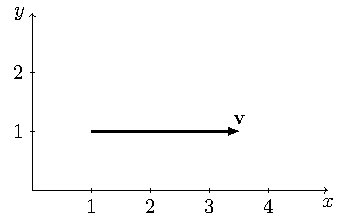
\includegraphics{vectorBaseAtPointOfAction}
\caption{سمتیہ}
\label{شکل_سمتیہ_دم_پر_عمل_درامد_ہوتی_ہے}
\end{figure}

\حصہ{سمتی الجبرا}
دو سمتیوں کا ترسیمی  مجموعہ حاصل کرنے کی خاطر ایک سمتیہ کے سر کو دوسری سمتیہ کے دُم  کے ساتھ ملایا جاتا ہے۔پہلی سمتیہ کی دُم سے دوسری سمتیہ کے سر تک سمتیہ حاصل جمع ہو گا۔اس عمل کو شکل \حوالہ{شکل_سمتیہ_سمتیوں_کا_مجموعہ}-الف میں دکھایا گیا ہے۔شکل میں \سمتیہ{A} کے سر کے ساتھ \سمتیہ{B} کی دُم ملائی گئی ہے۔دو سے زیادہ سمتیوں کا مجموعہ بھی اسی عمل کو استعمال کرتے  ہوئے حاصل کیا جاتا ہے۔اس عمل کو \اصطلاح{سر سے دُم جوڑنا}\فرہنگ{سر سے دُم جوڑنا}\فرہنگ{head to tail rule}\حاشیہب{head to tail rule} کہتے ہیں۔شکل \حوالہ{شکل_سمتیہ_سمتیوں_کا_مجموعہ}-ب میں دو سمتیوں کے دُم ملا کر سمتیوں کے متوازی الاضلاع\فرہنگ{متوازی الاضلاع}\حاشیہب{parallelogram law}\فرہنگ{parallelogram law}  سے ان کا مجموعہ حاصل کرنا دکھایا گیا ہے جسے دیکھ کر صاف ظاہر ہے کہ $\bf{A}+\bf{B}=\bf{B}+\bf{A}$ ہے یعنی سمتیوں کا مجموعہ قانون تبادل\فرہنگ{قانون تبادل}\حاشیہب{commutative law}\فرہنگ{commutative law} پر پورا اترتا ہے۔اسی طرح سمتیوں کا مجموعہ قانون تلازمی\فرہنگ{قانون تلازمی}\حاشیہب{associative law}\فرہنگ{associative law}
\begin{align}
\bf{A}+\left(\bf{B}+\bf{C}\right)=\left(\bf{A}+\bf{B}\right)+\bf{C}
\end{align}
 پر بھی پورا اترتا ہے۔
%  
\begin{figure}
\begin{subfigure}{0.5\textwidth}
\centering
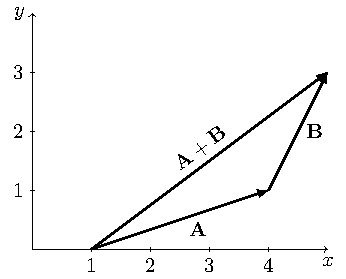
\includegraphics{figVectorHeadToTailRule}
\caption{سر کے ساتھ دُم جوڑ کر مجموعہ حاصل کیا جاتا ہے۔}
%\label{شکل_سمتیہ_سر_دم_جوڑنا}
\end{subfigure}
%
\begin{subfigure}{0.5\textwidth}
\centering
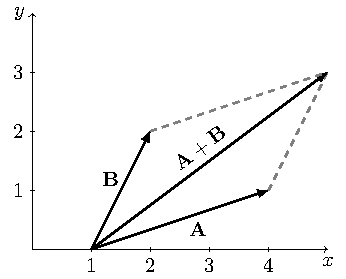
\includegraphics{figVectorParallelogramAdditionLaw}
\caption{متوازی الاضلاع سے بھی مجموعہ حاصل کیا جاتا ہے۔}
%\label{شکل_سمتیہ_متوازی_الاضلاع}
\end{subfigure}
\caption{سمتیوں کے مجموعے کا حصول}
\label{شکل_سمتیہ_سمتیوں_کا_مجموعہ}
\end{figure}

سمتیوں کے تفریق کا اصول  جمع کے اصول سے حاصل کیا جا سکتا ہے۔ہم $\bf{A}-\bf{B}$ کو $\bf{A}+\left(-\bf{B}\right)$ لکھ سکتے ہیں جہاں $-\bf{B}$ سے مراد یہ ہے کہ سمتیہ $\bf{B}$ کی سمت الٹی کر دی گئی ہے۔یوں $\bf{A}-\bf{B}$ حاصل کرنے کی خاطر $\bf{B}$ کی سمت الٹی کرتے ہوئے اس نئے سمتیہ کو $\bf{A}$ کے ساتھ جمع کیا جاتا ہے۔

سمتیہ \سمتیہ{A} کو مثبت  مقداری \عددیء{k} سے ضرب دینے سے سمتیہ کی سمت پر کوئی اثر نہیں ہوتا جبکہ اس کی لمبائی \عددیء{k} گنا ہو جاتی ہے۔اس کے برعکس سمتیہ \سمتیہ{A} کو منفی مقداری \عددیء{-k} سے ضرب دینے سے سمتیہ کی سمت الٹ ہو جاتی ہے اور اس کی لمبائی \عددیء{\abs{k}} گنا ہو جاتی ہے۔

دو سمتیے اُس صورت میں برابر ہوتے ہیں جب ان کا تفریق صفر کے برابر ہو یعنی \عددیء{\kvec{A}=\kvec{B}} تب ہو گا جب \عددیء{\kvec{A}-\kvec{B}=0} ہو۔

ہم سمتی میدان کے متغیرات کو آپس میں جمع یا منفی صرف اُس صورت کریں گے جب یہ متغیرات ایک ہی نقطے پر بیان کئے گئے ہوں۔یوں کسی بھی نقطے پر دو یا دو سے زیادہ مقناطیسوں کا اجتماعی مقناطیسی میدان حاصل کرتے ہوئے اس نقطے پر تمام مقناطیسوں کا علیحدہ علیحدہ مقناطیسی میدان لیتے ہوئے ان کا مجموعہ لیا جائے گا۔

اگر ہم سمتی میدان کی بات نہ کر رہے ہوں تب ہم مختلف مقامات پر پائے جانے والے سمتیوں کا بھی مجموعہ یا فرق لے سکتے ہیں۔یوں سمندر کے پانی میں ڈوبے  آب دوز کی اوپر اور نچلی سطح پر قوت کا مجموعہ حاصل کرتے ہوئے ہم یہ معلوم کر سکتے ہیں کہ آیا یہ مزید ڈوبے گا یا نہیں۔  

\حصہ{کارتیسی محدد}\شناخت{حصہ_سمتیہ_کارتیسی_محدد}
ایسا طریقہ جس سے کسی نقطے کا مقام بیان کیا جائے محدد\فرہنگ{محدد}\حاشیہب{coordinates}\فرہنگ{coordinates} کہلاتا ہے۔سیدھی سطح پر کسی بھی نقطے کو دو محدد سے ظاہر کیا جا سکتا ہے۔خلاء تین طرفہ\حاشیہب{three dimensional} ہے لہٰذا خلاء میں کسی بھی نقطے کو تین محدد سے ظاہر کیا جا سکتا ہے۔شکل \حوالہ{شکل_سمتیہ_اکائی_سے_سمتیہ_کا_اظہار}-الف میں دو طرفہ  \اصطلاح{کارتیسی} محدد پر اکائی لمبائی کے دو سمتیات \عددیء{\ax} اور \عددیء{\ay} دکھائے گئے ہیں۔اکائی سمتیہ \عددیء{\ax} کی سمت مثبت \عددیء{x} جانب کو ہے جبکہ \عددیء{\ay}  کی سمت مثبت \عددیء{y} جانب کو ہے۔شکل-ب میں \سمتیہ{A} دکھایا گیا ہے۔کسی بھی سمتیہ کو دو یا دو سے زیادہ سمتیوں کے مجموعے کی شکل میں لکھا جا سکتا ہے۔شکل میں \عددیء{\kvec{A}} کو \عددیء{\kvec{A}_x} اور \عددیء{\kvec{A}_y} کے مجموعے کی شکل میں دکھایا گیا ہے یعنی
\begin{align}
\kvec{A}=\kvec{A}_x+\kvec{A}_y
\end{align}

\begin{figure}
\begin{subfigure}{0.5\textwidth}
\centering
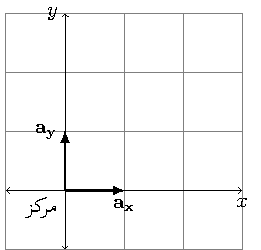
\includegraphics{unitVectorsInTwoDimensionalCartesianSpace}
\caption{اکائی سمتیہ}
%\label{شکل_سمتیہ_سر_دم_جوڑنا}
\end{subfigure}
%
\begin{subfigure}{0.5\textwidth}
\centering
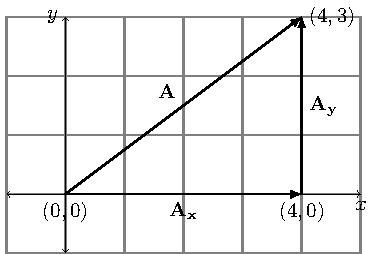
\includegraphics{vectorsRepresentationCartesianSpace}
\caption{اکائی سمتیوں کی مدد سے کسی بھی سمتیہ کو ظاہر کیا جا سکتا ہے۔}
%\label{شکل_سمتیہ_متوازی_الاضلاع}
\end{subfigure}
\caption{اکائی سمتیہ اور ان کا استعمال}
\label{شکل_سمتیہ_اکائی_سے_سمتیہ_کا_اظہار}
\end{figure}
%


زمین کی سطح کو لامحدود سیدھی سطح تصور کرتے ہوئے اس پر دو عمودی لکیریں کھینچتے ہوئے ایک لکیر کو \عددیء{x} محدد اور دوسری لکیر کو \عددیء{y} محدد تصور کیا جا سکتا ہے۔ایسی صورت میں اونچائی کو \عددیء{z} محدد سے ظاہر کیا جائے گا۔ اب اگر اونچائی صفر رکھتے ہوئے \عددیء{x} اور \عددیء{y} کو تبدیل کیا جائے تو ہم زمین کی سطح پر حرکت کریں گے۔اس طرح ہم دیکھتے ہیں کہ زمین کی سطح پر \عددیء{z=0} جبکہ اس پر \عددیء{x} اور \عددیء{y} آزاد متغیرات ہیں۔یوں زمین کی سطح کو \عددیء{z=0} سطح کہتے ہیں جسے
\begin{align*}
z=0, \quad  x\le \abs{\mp \infty}, \quad y \le \abs{\mp \infty}
\end{align*} 
لکھا جا سکتا ہے۔  شکل \حوالہ{شکل_سمتیہ_کارتیسی_نقطہ_اور_عمودی_سطحیں}-الف میں اس سطح کی نشاندہی کی گئی ہے۔ہم بالکل اسی طرح \عددیء{y=0} سطح اور \عددیء{x=0} سطح بھی بیان کر سکتے ہیں۔

\begin{figure}
\begin{subfigure}{0.5\textwidth}
\centering
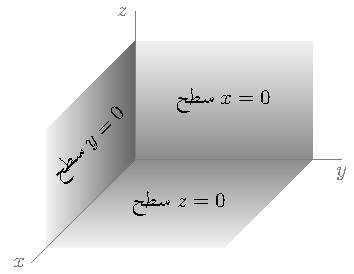
\includegraphics{figVectorPlaneSurfacesCartesian}
\caption{کارتیسی محدد میں عمودی سیدھی سطحیں۔}
\label{شکل_سمتیہ_کارتیسی_عمودی-تین_سطحیں}
\end{subfigure}
%
\begin{subfigure}{0.5\textwidth}
\centering
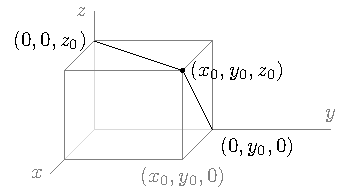
\includegraphics{figVectorPerpendicularsFromPointToCartesianAxis3D}
\caption{نقطے سے محدد پر عمود۔}
\label{شکل_سمتیہ_نقطے_سے_کارتیسی_محدد_پر_عمود}
\end{subfigure}
%
\caption{کارتیسی نظام میں نقطہ اور تین عمودی سطحیں۔}
\label{شکل_سمتیہ_کارتیسی_نقطہ_اور_عمودی_سطحیں}
\end{figure}
شکل  \حوالہ{شکل_سمتیہ_کارتیسی_نقطہ_اور_عمودی_سطحیں}-ب  کو دیکھتے ہوئے آگے  پڑھیں۔ کارتیسی محدد میں کسی بھی نقطے کو \عددیء{(x_0,y_0,z_0)} لکھا جا سکتا ہے۔اس نقطے تک پہنچنے کی خاطر  کارتیسی محدد کے مرکز سے پہلے \عددیء{x} محدد کے متوازی \عددیء{x_0}  فاصلہ طے کرتے ہوئے \عددیء{(x_0,0,0)} تک پہنچیں۔اس کے بعد \عددیء{y} محدد کے متوازی \عددیء{y_0} فاصلہ طے کرتے ہوئے \عددیء{(x_0,y_0,0)} تک پہنچیں  اور آخرکار \عددیء{z} محدد کے متوازی \عددیء{z_0} فاصلہ طے کرتے ہوئے درکار نقطہ \عددیء{(x_0,y_0,z_0)} تک پہنچیں۔اس عمل میں یہ ضروری نہیں کہ پہلے \عددیء{x} محدد کے متوازی ہی چلا جائے۔آپ مرکز سے پہلے \عددیء{y} محدد کے متوازی \عددیء{y_0} فاصلہ طے کرنے کے بعد \عددیء{z} محدد کے متوازی \عددیء{z_0} اور آخرکار \عددیء{x} محدد کے متوازی \عددیء{x_0} فاصلہ طے کرتے ہوئے بھی اسی نقطے تک پہنچ سکتے ہیں۔تینوں فاصلوں کو کسی بھی ترتیب سے طے کیا جا سکتا ہے۔

 نقطہ \عددیء{(x_0,y_0,z_0)} سے \عددیء{x} محدد پر عمود بناتے ہوئے  \عددیء{(x_0,0,0)} حاصل ہوتا ہے۔اسی طرح اس نقطے سے \عددیء{y} محدد پر عمود \عددیء{(0,y_0,0)} اور \عددیء{z} محدد پر عمود \عددیء{(0,0,z_0)} دیتا ہے۔نقطہ \عددیء{(x_0,y_0,z_0)} سے \عددیء{y} محدد اور \عددیء{z} محدد پر عمودی لکیریں گہری سیاہی میں دکھائے گئے ہیں۔ اگر \عددیء{(x_0,y_0,z_0)} سے  شروع ہوتے ہوئے \عددیء{z} محدد کے متوازی یوں چلا جائے کہ آخرکار \عددیء{z=0} ہو جائے تو نقطہ \عددیء{(x_0,y_0,0)} حاصل ہو گا۔ اب اگر یہاں سے \عددیء{x} محدد کے متوازی یوں چلا جائے کہ آخرکار \عددیء{x=0} ہو جائے تو نقطہ \عددیء{(0,y_0,0)} حاصل ہو گا۔یہ وہی نقطہ ہے جو \عددیء{(x_0,y_0,z_0)} سے \عددیء{y} محدد پر عمودی لکیر بناتے ہوئے حاصل ہوتا ہے۔اس عمل میں ہم پہلے \عددیء{x} محدد کے متوازی چلتے ہوئے \عددیء{x=0} کرنے کے بعد \عددیء{z} محدد کے متوازی چلتے ہوئے \عددیء{z=0} کرتے ہوئے بھی نقطہ \عددیء{(0,0,y_0)} تک پہنچ سکتے تھے۔

نقطہ \عددیء{(x_0,y_0,z_0)} تک قدر مختلف انداز سے بھی پہنچا جا سکتا ہے جسے کارتیسی محدد میں سمجھنا زیادہ آسان ہے۔فرض کریں کہ \عددیء{x=x_0} پر لامحدود \عددیء{yz} سیدھی سطح بنائی جائے۔ایسی سطح کو \عددیء{x=x_0} سطح  کہتے ہیں۔اس سطح کو
\begin{align*}
x=x_0, \quad  y\le \abs{\mp \infty}, \quad z \le \abs{\mp \infty}
\end{align*} 
لکھا جا سکتا ہے۔اس مساوات میں \عددیء{x_0} مقررہ ہے جبکہ \عددیء{y} اور \عددیء{z} متغیرات ہیں۔دو متغیرات کی مساوات سطح کو ظاہر کرتی ہے۔اگر \عددیء{y=y_0} پر لامحدود \عددیء{xz} سیدھی سطح بنائی جائے تو یہ دو سطحے  آپس میں سیدھی لکیر پر ملیں گے۔یہ لکیر
\begin{align*}
x=x_0, \quad  y=y_0, \quad z \le \abs{\mp \infty}
\end{align*} 
لکھی جا سکتی ہے۔اس مساوات میں \عددیء{x_0} اور \عددیء{y_0} مقررہ ہیں جبکہ \عددیء{z} متغیرہ ہے۔ایک متغیرہ کی مساوات لکیر کو ظاہر کرتی ہے۔اب اگر \عددیء{z=z_0} پر لامحدود \عددیء{xy} سیدھی سطح بھی بنائی جائے تب یہ تینوں سطحے ایک نقطے \عددیء{N(x_0,y_0,z_0)} پر آپس کو چھوئنگے۔یہ صورت حال شکل \حوالہ{شکل_سمتیہ_تین_عمودی_سطحوں_سے_نقطہ} میں دکھائی گئی ہے جہاں لامحدود سطحوں کے کچھ حصے دکھائے گئے ہیں۔آپ دیکھیں گے کہ نقطے تک پہنچنے کا یہ طریقہ دیگر محدد میں استعمال کرنا لازمی ثابت ہو گا۔
\begin{figure}
\centering
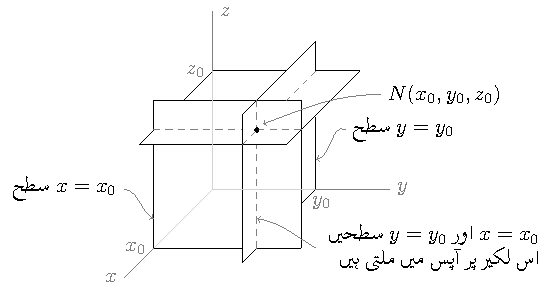
\includegraphics{figVectorLineAsSurfacesTouching}
\caption{تین عمودی سطحوں سے نقطے کا حصول۔}
\label{شکل_سمتیہ_تین_عمودی_سطحوں_سے_نقطہ}
\end{figure}

اگر سطح \عددیء{x=x_0}  کے متوازی \عددیء{x=x_0+\dif x} پر اور اسی طرح \عددیء{y=y_0} کے متوازی \عددیء{y=y_0+\dif y} اور \عددیء{z=z_0} کے متوازی \عددیء{z=z_0+\dif z} سطح رکھے جائیں تو یہ چھ سطحے ایک چھوٹی  مکعب نما حجم  کو گھیریں گی جسے شکل \حوالہ{شکل_سمتیہ_کارتیسی_چھوٹی_مکعب} میں دکھایا گیا ہے جبکہ یہ تین نئی سطحیں آپس میں نقطہ \عددیء{N'(x_0+\dif x,y_0+\dif y,z_0+\dif z)} پر ملیں گی ۔
\begin{figure}
\centering
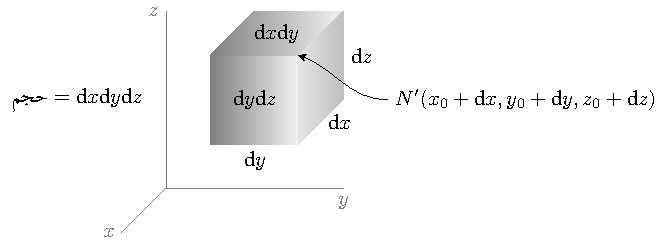
\includegraphics{figVectorCubeShaded}
\caption{چھ سطحے مکعب گھیرتی ہیں۔}
\label{شکل_سمتیہ_کارتیسی_چھوٹی_مکعب}
\end{figure}
اس مکعب نما کے اطراف \عددیء{\dif x}، \عددیء{\dif y} اور \عددیء{\dif z} ہیں۔ اس کی اوپر والی سطح کا رقبہ \عددیء{\dif x \dif y} ہے۔اسی طرح اس کی نچلی سطح کا رقبہ بھی \عددیء{\dif x \dif y} ہے۔سامنے سطح  اور پچھلی سطح دونوں \عددیء{\dif y \dif z} رقبے رکھتے ہیں جبکہ بائیں  اور دائیں سطحوں کے رقبے \عددیء{\dif x \dif z} کے برابر ہیں۔اس مکعب نما کی حجم \عددیء{\dif x \dif y \dif z} ہے۔نقطہ \عددیء{N'(x_0+\dif x,y_0+\dif y,z_0+\dif z)} شکل میں دکھایا گیا ہے جبکہ
 نقطہ \عددیء{N(x_0,y_0 ,z_0)} مکعب نما کا وہ واحد کونا ہے جسے شکل میں نہیں دکھایا گیا۔ان دو نقطوں کے درمیان فاصلہ \عددیء{NN'=\sqrt{\dif x^2+\dif y^2+\dif z^2}} ہے۔ 
%==================
\حصہ{اکائی سمتیات}
حصہ  \حوالہ{حصہ_سمتیہ_کارتیسی_محدد} کے شروع میں دو طرفہ کارتیسی نظام  میں سیدھی سطح پر کسی بھی سمتیہ کو دو سمتیات کی صورت میں لکھنا دکھایا گیا۔یہی طریقہ تین طرفہ کارتیسی نظام کے لئے بھی استعمال کیا جاتا ہے۔ تین طرفہ کارتیسی نظام کے تین اکائی سمتیات \عددیء{\ax}، \عددیء{\ay} اور \عددیء{\az} لکھے جاتے ہیں۔یہ تینوں سمتیات آپس میں عمودی ہیں۔کسی بھی اکائی سمتیہ کی طرح یہ تین اکائی سمتیات اکائی لمبائی رکھتے ہیں۔ \عددیء{\ax} کی سمت \عددیء{x} محدد کے بڑھتے جانب کو ہے۔اسی طرح \عددیء{\ay} کی سمت \عددیء{y} محدد کے بڑھتے جانب کو اور \عددیء{\az} کی سمت \عددیء{z} محدد کے بڑھتے جانب کو ہے۔شکل \حوالہ{شکل_سمتیہ_کارتیسی_تین_اکائی_سمتیات}-الف میں یہ تینوں اکائی سمتیات دکھائے گئے ہیں۔اسی شکل میں نقطہ \عددیء{(0,1,2)} پر سمتیہ دکھایا گیا ہے جس کی لمبائی دو کے برابر ہے جبکہ یہ اکائی سمتیہ \عددیء{\ay} کی سمت میں ہے۔اس سمتیہ کو \عددیء{2\ay} لکھا جا سکتا ہے۔یاد رہے کہ ایسے دو سمتیات برابر ہوتے ہیں جن کا طول برابر ہو اور جو ایک ہی سمت میں ہوں۔ یوں سمت تبدیل کئے بغیر سمتیہ کو کارتیسی محدد کے مرکز منتقل کرتے ہوئے اس کی قیمت نسبتاً آسانی سے لکھی جا سکتی ہے۔
\begin{figure}
\centering
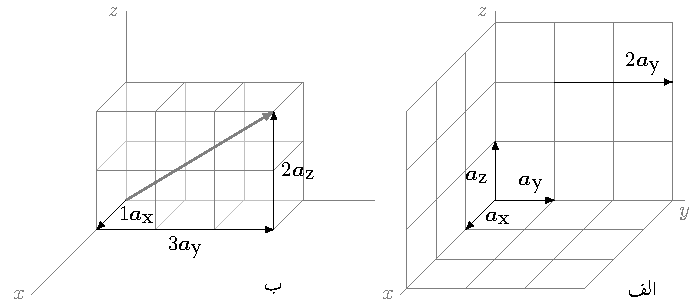
\includegraphics{figVector3DUnitVectors}
\caption{کارتیسی نظام کے اکائی سمتیات اور ان کا استعمال}
\label{شکل_سمتیہ_کارتیسی_تین_اکائی_سمتیات}
\end{figure}
%
\begin{figure}
\centering
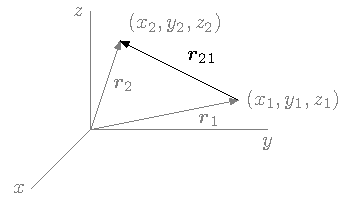
\includegraphics{figVector3DcartesianVectorEquation}
\caption{کارتیسی نظام میں سمتیہ کی مساوات کا حصول}
\label{شکل_سمتیہ_کارتیسی_سمتیہ_کی_مساوات}
\end{figure}
%
\begin{figure}
\centering
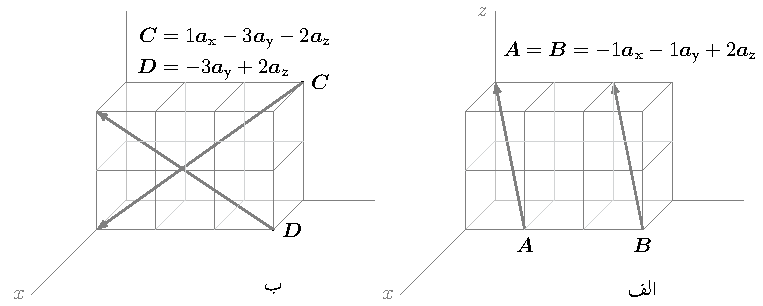
\includegraphics{figVector3DcartesianVectors}
\caption{کارتیسی نظام میں چند سمتیات}
\label{شکل_سمتیہ_کارتیسی_چند_سمتیات}
\end{figure}
%

شکل \حوالہ{شکل_سمتیہ_کارتیسی_سمتیہ_کی_مساوات} میں  مرکز سے \عددیء{(x_1,y_1,z_1)} تک سمتیہ \عددیء{\kvec{r}_1=x_1 \ax+y_1\ay+z_1\az} اور  مرکز سے \عددیء{(x_2,y_2,z_2)} تک سمتیہ \عددیء{\kvec{r}_2=x_2 \ax+y_2\ay+z_2\az} دکھائے گئے ہیں۔شکل میں سمتیہ \عددیء{\kvec{r}_{21}} بھی دکھائی گئی ہے جس کی دُم  \عددیء{(x_1,y_1,z_1)} اور  نوک \عددیء{(x_2,y_2,z_2)} پر ہے۔ سر سے دُم جوڑنے کے اصول کے استعمال سے \عددیء{\kvec{r}_2=\kvec{r}_{21}+\kvec{r}_1} لکھا جا سکتا ہے جس سے 
\begin{gather}
\begin{aligned}\label{مساوات_سمتیہ_کارتیسی_نظام_میں_قیمت}
\kvec{r}_{21}&=\kvec{r}_2-\kvec{r}_1\\
&=(x_2-x_1) \ax+(y_2-y_1)\ay+(z_2-z_1)\az
\end{aligned}
\end{gather}
حاصل ہوتا ہے۔اس مساوات کے استعمال سے سمتیہ کی مساوات باآسانی حاصل ہوتی ہے۔سمتیہ \عددیء{\kvec{r}_{21}} لکھتے ہوئے زیرنوشت میں سمتیہ کی نوک کو \عددیء{2} اور اس کی دُم  کو \عددیء{1} سے ظاہر کیا گیا ہے۔اس کتاب میں سمتیہ لکھتے ہوئے نوک اور دُم  کو اسی ترتیب سے زیرنوشت میں لکھا جائے گا۔یوں سمتیہ \عددیء{\kvec{r}_{21}} کو تین اجزاء \عددیء{(x_2-x_1)\ax}، \عددیء{(y_2-y_1)\ay} اور \عددیء{(z_2-z_1)\az} کے مجموعے کی شکل میں لکھا جا سکتا ہے۔

شکل \حوالہ{شکل_سمتیہ_کارتیسی_تین_اکائی_سمتیات}-ب میں مرکز سے \عددیء{(1,3,2)} تک سمتیہ دکھایا گیا ہے۔آپ دیکھ سکتے ہیں کہ اس کو تین سمتیات کا مجموعہ لکھا جا سکتا ہے یعنی \عددیء{1\ax+3\ay+2\az} جہاں اکائی سمتیات استعمال کرتے ہوئے تینوں اجزاء کو لکھا گیا ہے۔ سمتیہ کی دُم \عددیء{(0,0,0)} اور اس کی نوک \عددیء{(1,3,2)} پر لیتے ہوئے  یہی جواب  مساوات \حوالہ{مساوات_سمتیہ_کارتیسی_نظام_میں_قیمت} سے بھی حاصل ہوتا ہے۔

شکل \حوالہ{شکل_سمتیہ_کارتیسی_چند_سمتیات}-الف میں دو متوازی سمتیات \عددیء{\kvec{A}} اور \عددیء{\kvec{B}} دکھائے ہیں جن کی لمبائی برابر ہے۔ چونکہ ان کی لمبائی برابر ہے اور یہ دونوں ایک ہی سمت میں ہیں لہٰذا \عددیء{\kvec{A}=\kvec{B}=-1\ax-1\ay+2\az} لکھا جائے گا۔شکل \حوالہ{شکل_سمتیہ_کارتیسی_چند_سمتیات}-ب میں \عددیء{\kvec{C}} کی دُم سے \عددیء{\ax} جانب ایک قدم اور یہاں سے \عددیء{-\ay} جانب تین قدم اور آخرکار \عددیء{-\az} جانب دو قدم چلنے سے اس کی نوک تک پہنچا جا سکتا ہے لہٰذا \عددیء{\kvec{C}=1\ax-3\ay-2\az} لکھا جائے گا۔ اسی طرح \عددیء{\kvec{D}} کی دُم سے  \عددیء{-\ay} جانب تین قدم اور پھر \عددیء{\az} جانب دو قدم چلتے ہوئےسمتیہ کی نوک تک پہنچا جایا سکتا ہے لہٰذا \عددیء{\kvec{D}=-3\ay+2\az} لکھا جائے گا۔سمتیہ \عددیء{\kvec{D}} کو دو اجزاء کی شکل میں لکھا گیا ہے چونکہ اس کے تیسرے جزو کی لمبائی صفر کے برابر ہے۔
%=====================
\ابتدا{مشق}
مساوات \حوالہ{مساوات_سمتیہ_کارتیسی_نظام_میں_قیمت} کے استعمال سے شکل \حوالہ{شکل_سمتیہ_کارتیسی_چند_سمتیات} میں تمام سمتیات لکھیں۔

جوابات:تمام جوابات شکل میں دئے گئے ہیں۔
\انتہا{مشق}
%======================
\begin{figure}
\centering
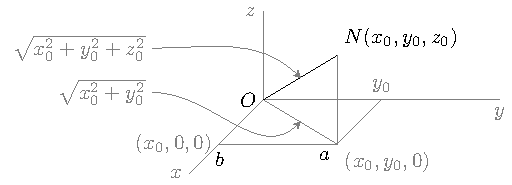
\includegraphics{figVectorCartesianAmplitudeFromPythagorousTheorem}
\caption{کارتیسی نظام میں سمتیہ کا طول}
\label{شکل_سمتیہ_کارتیسی_سمتیہ_طول}
\end{figure}

شکل \حوالہ{شکل_سمتیہ_کارتیسی_سمتیہ_طول} میں مرکز سے نقطہ \عددیء{N(x_0,y_0,z_0)} تک کا فاصلہ \عددیء{ON} مسئلہ \اصطلاح{فیثاغورث}\فرہنگ{فیثاغورث}\حاشیہب{Pythagoras theorem}\فرہنگ{Pythagoras theorem} سے حاصل کیا جا سکتا ہے۔اس نقطے سے \عددیء{z=0} سطح پر عمود سے نقطہ \عددیء{a} حاصل ہوتا ہے۔نقطہ \عددیء{a} سے \عددیء{x} محدد پر عمود نقطہ \عددیء{b} دیتا ہے۔تکون \عددیء{Oba} میں \عددیء{O} سے \عددیء{b} کا فاصلہ \عددیء{x_0} ہے جبکہ \عددیء{b} سے \عددیء{a} کا فاصلہ \عددیء{y_0} ہے۔یوں فاصلہ \عددیء{Oa} مسئلہ فیثاغورث کی مدد سے  \عددیء{\sqrt{x_0^2+y_0^2}} کے برابر ہو گا۔ تکون \عددیء{OaN} میں \عددیء{a} پر \عددیء{90^{\circ}} کا زاویہ پایا جاتا ہے۔یوں مسئلہ فیثاغورث کی مدد سے \عددیء{ON} کا فاصلہ \عددیء{\sqrt{x_0^2+y_0^2+z_0^2}} حاصل ہوتا ہے۔

مساوات \حوالہ{مساوات_سمتیہ_کارتیسی_نظام_میں_قیمت} سمتیہ کی عمومی مساوات ہے۔اس میں دئے سمتیہ \عددیء{\kvec{r}_{21}} کی دُم محدد کے مرکز پر رکھنے سے صاف ظاہر ہے کہ سمتیہ کی مقدار
\begin{align}
\abs{\kvec{r}_{21}}=r_{21}=\sqrt{(x_2-x_1)^2+(y_2-y_1)^2+(z_2-z_1)^2}
\end{align}
کے برابر ہے۔اگر سمتیہ کو اس کی مقدار سے تقسیم کیا جائے تو حاصل جواب کی مقدار اکائی ہو گی جبکہ اس کی سمت میں کوئی تبدیلی رونما نہیں ہو گی۔یوں  \عددیء{\kvec{r}_{21}} کو \عددیء{\abs{\kvec{r}_{21}}} سے تقسیم کرتے ہوئے \عددیء{\kvec{r}_{21}} کی سمت میں اکائی سمتیہ \عددیء{\kvec{a}_{r21}} حاصل کی جا سکتی ہے۔
\begin{align}
\kvec{a}_{r21}=\frac{\kvec{r}_{21}}{\abs{\kvec{r}_{21}}}=\frac{(x_2-x_1) \ax+(y_2-y_1)\ay+(z_2-z_1)\az}{\sqrt{(x_2-x_1)^2+(y_2-y_1)^2+(z_2-z_1)^2}}
\end{align}
یاد رہے کہ سمتیہ کی سمت اور طول تبدیل کئے بغیر اسے ایک مقام سے دوسری مقام منتقل کیا جا سکتا ہے۔البتہ وہ سمتیہ جو کسی نقطے کی مقام تعین کرتا ہو کو اگر کہیں اور منتقل کیا جائے تو ایسی صورت میں  سمتیہ کی نوک درکار نقطے پر نہیں رہے گی۔اسی حقیقت کی بنا پر میدان ظاہر کرنے والے سمتیہ کو اپنی جگہ سے نہیں ہٹایا جا سکتا۔میدانی سمتیہ کی دُم اس مقام پر پائی جاتی ہے جہاں میدان بیان کی جا رہی ہو۔  

سمتیات کے استعمال سے نقطہ \عددیء{(x,y,z)} کے مقام کو \عددیء{\kvec{r}=x\ax+y\ay+z\az} لکھا جاتا ہے۔کسی بھی سمتیہ مثلاً قوت \عددیء{\kvec{F}} کو بالکل اسی طرح  \عددیء{\kvec{F}=F_x\ax+F_y\ay+F_z\az} لکھا جاتا ہے جہاں \عددیء{F_x \ax}، \عددیء{F_y \ay} اور \عددیء{F_z\az} اس کے تین اجزاء ہیں۔اس طرح قوت کی مقدار  \عددیء{\abs{\kvec{F}}=\sqrt{F_x^2+F_y^2+F_z^2}} کے برابر ہو گی۔
%======================
\ابتدا{مثال}
نقطہ \عددیء{(-5,2,-1)}  کا مقام ظاہر کرنے والا سمتیہ اور اس سمتیہ کا طول حاصل کریں۔اسی سمتیہ کی سمت میں اکائی سمتیہ حاصل کریں۔

حل:مرکز سے اس نقطے تک کا سمتیہ \عددیء{\kvec{r}=-5\ax+2\ay-1\az} ہے جبکہ اس سمتیہ  کا طول \عددیء{\abs{\kvec{r}}=\sqrt{5^2+2^2+1^1}=\sqrt{30}} ہے۔یوں اکائی سمتیہ \عددیء{\kvec{a}_r=\tfrac{-5\ax+2\ay-1\az}{\sqrt{30}}} ہو گا۔
\انتہا{مثال}
%=====================

\ابتدا{مثال}\شناخت{مثال_سمتیہ_نقطے_سے_درمیان_تک_سمتیہ}
شکل \حوالہ{شکل_سمتیہ_استعمال_سمتیہ_مثال} میں تین نقطے \عددیء{M(1,6,4)}، \عددیء{N(4,5,1)} اور \عددیء{P(1,2,2)} دئے گئے ہیں۔\عددیء{M} اور \عددیء{N} کے درمیان سیدھی لکیر پر \عددیء{M} سے کل فاصلے کے  \عددیء{\tfrac{1}{3}} پر نقطہ \عددیء{Q} پایا جاتا ہے۔\عددیء{Q} سے \عددیء{P} تک سمتیہ حاصل کرتے ہوئے ان دو نقطوں کے درمیان فاصلہ معلوم کریں۔
\begin{figure}
\centering
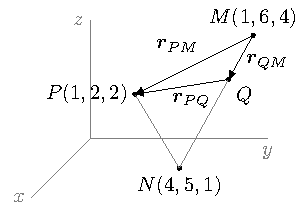
\includegraphics{figVectorExampleA}
\caption{سمتیوں کا استعمال}
\label{شکل_سمتیہ_استعمال_سمتیہ_مثال}
\end{figure}
حل:\عددیء{M} سے \عددیء{N} تک سمتیہ
\begin{align*}
\kvec{r}_{NM}&=(4-1)\ax+(5-6)\ay+(1-4)\az\\
&=3\ax-1\ay-3\az
\end{align*}
ہے۔\عددیء{M} سے \عددیء{Q} تک سمتیہ \عددیء{\kvec{r}_{QM}} اور \عددیء{\kvec{r}_{NM}} ایک ہی سمت میں ہیں جبکہ \عددیء{\abs{\kvec{r}_{QM}}=\tfrac{1}{3}\abs{\kvec{r}_{NM}}} کے برابر ہے۔یوں
\begin{align*}
\kvec{r}_{QM}=\frac{1}{3}\kvec{r}_{NM}=\frac{1}{3}(3\ax-1\ay-3\az)=1\ax-\frac{1}{3}\ay-1\az
\end{align*}
ہو گا۔\عددیء{M} سے \عددیء{P} تک سمتیہ
\begin{align*}
\kvec{r}_{PM}&=(1-1)\ax+(2-6)\ay+(2-4)\az\\
&=-4\ay-2\az
\end{align*}
ہے۔شکل کو دیکھتے ہوئے ہم لکھ سکتے ہیں \عددیء{\kvec{r}_{QM}+\kvec{r}_{PQ}=\kvec{r}_{PM}} لہٰذا
\begin{align*}
\kvec{r}_{PQ}&=\kvec{r}_{PM}-\kvec{r}_{QM}\\
&=(-4\ay-2\az)-(1\ax-\frac{1}{3}\ay-1\az)\\
&=-1\ax-\frac{11}{3}\ay-1\az
\end{align*}
ہو گا۔\عددیء{Q} سے \عددیء{P} تک فاصلہ \عددیء{\sqrt{1^1+\left(\tfrac{11}{3}\right)^2+1^2}=3.93} ہے۔
\انتہا{مثال}
%===================
\ابتدا{مشق}
مثال \حوالہ{مثال_سمتیہ_نقطے_سے_درمیان_تک_سمتیہ} میں دئے نقطوں کو استعمال کرتے ہوئے \عددیء{M} سے \عددیء{P} تک سمتیہ حاصل کریں۔اسی طرح \عددیء{P} سے \عددیء{N} تک سمتیہ اور \عددیء{M} سے \عددیء{N} تک سمتیہ حاصل کریں۔پہلے دو جوابات کو استعمال کرتے ہوئے \اصطلاح{سر سے دُم جوڑنے} کے اصول سے تیسرا سمتیہ دوبارہ حاصل کریں۔

جوابات:\عددیء{-5\ax-4\ay} ، \عددیء{-1\ax+4\ay+12\az} اور \عددیء{-6\ax+12\az}

\انتہا{مشق}


\حصہ{میدانی سمتیہ}\حاشیہط{لکھنا ہے}

\حصہ{سمتی رقبہ}
کسی بھی سطح کے دو اطراف ہوتے ہیں۔یوں سطح کے کسی بھی نقطے پر دو آپس میں الٹ سمتوں میں عمود بنائے جا سکتے ہیں۔سیدھی سطح جس کا رقبہ \عددیء{S} ہو کے ایک طرف پر اکائی عمود \عددیء{\kvec{a}_N} اور دوسری طرف پر اکائی عمود \عددیء{-\kvec{a}_N} بنائے جا سکتے ہیں۔اگر ان دو عمود میں سے ایک عمود مثلاً \عددیء{\kvec{a}_N} کو سطح کی سمت\حاشیہد{عمود سطح کے ساتھ نوے درجہ زاویہ بناتا ہے۔\عددیء{\kvec{a}_N} کے زیر نوشت میں \عددیء{N}، لفظ \موٹا{نوے} کے پہلے حرف کی آواز کو ظاہر کرتا ہے۔} تصور کیا جائے تب اس سطح کا \اصطلاح{سمتی رقبہ}\فرہنگ{سمتی رقبہ}\حاشیہب{vector area}\فرہنگ{vector area} \عددیء{S\kvec{a}_N} ہو گا۔بند سطح کے  بیرونی اکائی عمود کو سطح کی سمت تصور کیا جاتا ہے۔شکل \حوالہ{شکل_سمتیہ_سمتی_رقبہ} میں سمتی رقبے \عددیء{\kvec{A}_1} اور \عددیء{\kvec{A}_2} دکھائے گئے ہیں جہاں بند سطح کے بیرونی عمود کو ہی سطح کی سمت دکھایا گیا ہے۔
\begin{figure}
\centering
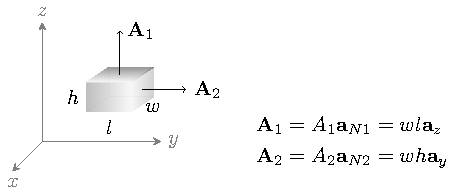
\includegraphics{figVectorVectorArea}
\caption{سمتی رقبہ}
\label{شکل_سمتیہ_سمتی_رقبہ}
\end{figure}


\حصہ{غیر سمتی ضرب}
دو سمتیات \عددیء{\kvec{A}} اور \عددیء{\kvec{B}} کے \اصطلاح{غیر سمتی ضرب}\فرہنگ{غیر سمتی ضرب}\فرہنگ{نقطہ ضرب}\فرہنگ{مقداری ضرب}\حاشیہب{scalar product}\فرہنگ{scalar product} سے مراد \عددیء{\kvec{A}} کی مقدار ضربِ  \عددیء{\kvec{B}} کی مقدار ضربِ سمتیوں کے مابین چھوٹے زاویے کا کوسائن ہے۔
\begin{align}\label{مساوات_سمتیہ_مقداری_ضرب}
\kvec{A} \cdot \kvec{B}=\abs{\kvec{A}} \abs{\kvec{B}} \cos \theta_{AB}
\end{align}

اگر دونوں سمتیات کی دُم ایک ہی جگہ پر نہ ہو تب ان کے مابین زاویہ دریافت کرنے کی  خاطر سمتیوں کی سمت تبدیل کئے بغیر انہیں ایک نقطے پر منتقل کیا جا سکتا ہے۔غیر سمتی ضرب دو سمتیوں کے مابین کیا جاتا ہے جبکہ اس کا حاصل جواب مقداری ہوتا ہے جس کی وجہ سے اسے  \اصطلاح{مقداری ضرب} بھی کہا جاتا ہے۔غیر سمتی ضرب کو سمتیوں کے درمیان نقطے سے ظاہر کیا جاتا ہے۔اسی وجہ سے اسے \اصطلاح{ضرب نقطہ}\حاشیہب{dot product}\فرہنگ{dot product} بھی کہا جاتا ہے۔ یوں \عددیء{\kvec{A} \cdot \kvec{B}} کو "\عددیء{\kvec{A}}نقطہ \عددیء{\kvec{B}}" پڑھا جاتا ہے۔بالکل سادہ ضرب کی طرح \عددیء{\kvec{A} \cdot \kvec{B}} کو \عددیء{\kvec{B} \cdot \kvec{A}} بھی لکھا جا سکتا ہے یعنی غیر سمتی ضرب میں متغیرات کی ترتیب اہمیت نہیں رکھتی۔

کارتیسی اکائی سمتیات \عددیء{\ax}، \عددیء{\ay} اور \عددیء{\az} آپس میں عمودی ہیں لہٰذا ان میں کسی بھی دو سمتیات کے درمیان \عددیء{90 \degree} زاویہ پایا جاتا ہے۔چونکہ \عددیء{\cos 90=0} کے برابر ہوتا ہے لہٰذا ان میں کسی بھی دو سمتیوں کا غیر سمتی ضرب صفر کے برابر ہوتا ہے یعنی
\begin{align}\label{مساوات_سمتیہ_عمودی_نقطہ_ضرب_برابر_صفر_اجزاء}
\ax \cdot \ay =0, \quad \ax \cdot \az=0, \quad \ay \cdot \az=0
\end{align}
ایک ہی سمت میں دو سمتیوں کے درمیان صفر زاویہ ہوتا ہے اور \عددیء{\cos 0=1} کے برابر ہے۔ اکائی سمتیہ کا طول بھی ایک کے برابر ہے لہٰذا مساوات \حوالہ{مساوات_سمتیہ_مقداری_ضرب} کے تحت \عددیء{\ax} اور \عددیء{\ax} کا غیر سمتی ضرب
\begin{align*}
\ax \cdot \ax=(\abs{\ax})(\abs{\ax})(\cos 0\degree)=(1)(1)(1)=1
\end{align*}
ہو گا۔بقایا دو کارتیسی اکائی سمتیات کا خود غیر سمتی ضرب بھی ایک کے برابر ہے۔
\begin{align}\label{مساوات_سمتیہ_عمودی_نقطہ_ضرب_برابر_ایک_اجزاء}
\ax \cdot \ax=1, \quad \ay \cdot \ay=1, \quad \az \cdot \az=1
\end{align}
مساوات \حوالہ{مساوات_سمتیہ_عمودی_نقطہ_ضرب_برابر_صفر_اجزاء} اور مساوات \حوالہ{مساوات_سمتیہ_عمودی_نقطہ_ضرب_برابر_ایک_اجزاء} کو \اصطلاح{کرونیکر ڈیلٹا}\فرہنگ{کرونیکر ڈیلٹا}\حاشیہد{یہ لیوپولڈ کرونیکر کے نام سے  منسوب ہے۔} \عددیء{\delta_{ij}} کی مدد سے ایک ہی مساوات کی مدد سے یوں لکھا جا سکتا ہے۔
\begin{align}
\kvec{a}_i \cdot \kvec{a}_j=\delta_{ij}
\end{align}
جہاں
\begin{align}
\delta_{ij}=
\begin{cases}
0 \quad  \quad  i\ne j \; \textup{ اگر}\\
1 \quad \quad i=j \; \textup{ اگر}
\end{cases}
\end{align}
کے برابر ہے یعنی \عددیء{i=j} کی صورت میں ہی \عددیء{\delta_{ij}} کی قیمت ایک  جبکہ \عددیء{i\ne j} کی صورت میں ہی \عددیء{\delta_{ij}} کی قیمت صفر کے برابر لی جاتی ہے۔یوں \عددیء{\ax \cdot \ay} کی صورت میں \عددیء{i=\ax} جبکہ \عددیء{j=\ay} کے برابر ہیں۔یوں \عددیء{i} اور \عددیء{j} برابر نہیں ہیں لہٰذا حاصل جواب صفر کے برابر ہو گا۔اس کے برعکس \عددیء{\az \cdot \az} کی صورت میں \عددیء{i=\az} اور \عددیء{j=\az} ہیں لہٰذا \عددیء{i=j} ہے اور یوں حاصل جواب ایک کے برابر ہے۔

کارتیسی تین عمودی اکائیوں کی مدد سے سمتیات کا غیر سمتی ضرب نہایت آسانی سے حاصل ہوتا ہے۔یوں اگر \عددیء{\kvec{A}=A_x\ax+A_y\ay+A_z\az} اور  \عددیء{\kvec{B}=B_x\ax+B_y\ay+B_z\az}  دو سمتیات ہوں تب ان کا غیر سمتی ضرب
\begin{align*}
\kvec{A} \cdot \kvec{B}&=(A_x\ax+A_y\ay+A_z\az) \cdot (B_x\ax+B_y\ay+B_z\az)\\
&=A_x B_x \ax \cdot \ax+A_x B_y \ax \cdot \ay+A_x B_z \ax \cdot \az\\
& \quad \quad +A_y B_x \ay \cdot \ax+A_y B_y \ay \cdot \ay+A_y B_z \ay \cdot \az \\
&\quad \quad +A_z B_x \az \cdot \ax+A_z B_y \az \cdot \ay+A_z B_z \az \cdot \az
\end{align*}
ہو گا۔مساوات \حوالہ{مساوات_سمتیہ_عمودی_نقطہ_ضرب_برابر_صفر_اجزاء} اور مساوات \حوالہ{مساوات_سمتیہ_عمودی_نقطہ_ضرب_برابر_ایک_اجزاء} کا سہارا لیتے ہوئے یوں
\begin{align}\label{مساوات_سمتیہ_نقطہ_ضرب_بمدد_اکائی_سمتیات}
\kvec{A} \cdot \kvec{B}=A_x B_x+A_y B_y+ A_z B_z
\end{align}
حاصل ہوتا ہے۔اس مساوات سے ہم دیکھتے ہیں کہ سمتیہ \عددیء{\kvec{A}} کا خود غیر سمتی ضرب 
\begin{align}
\kvec{A} \cdot \kvec{A} =A_x^2+A_y^2+ A_z^2=\abs{\kvec{A}}^2
\end{align}
اس کے طول کے مربع کے برابر ہے۔یہ انتہائی اہم نتیجہ ہے جسے عموماً استعمال کرتے ہوئے سمتیہ کا طول حاصل کیا جاتا ہے۔

مساوات \حوالہ{مساوات_سمتیہ_مقداری_ضرب} اور مساوات \حوالہ{مساوات_سمتیہ_نقطہ_ضرب_بمدد_اکائی_سمتیات} کی مدد سے دو سمتیوں کے مابین زاویہ معلوم کیا جا سکتا ہے یعنی
\begin{align}
\theta_{AB}=\cos^{-1}\left(\frac{\kvec{A} \cdot \kvec{B}}{(\kvec{A} \cdot \kvec{A})(\kvec{B} \cdot \kvec{B})}\right)=\cos^{-1} \left(\frac{A_x B_x+A_y B_y+ A_z B_z}{\sqrt{A_x^2+A_y^2+A_z^2} \sqrt{B_x^2+B_y^2+B_z^2}} \right)
\end{align}
%==================
\ابتدا{مثال}
شکل \حوالہ{شکل_سمتیہ_استعمال_سمتیہ_مثال} میں تکون دکھایا گیا ہے جس کے نوک  \عددیء{M(1,6,4)}، \عددیء{N(4,5,1)} اور \عددیء{P(1,2,2)}  ہیں۔\عددیء{M} پر زاویہ حاصل کریں۔

حل:مثال  \حوالہ{مثال_سمتیہ_نقطے_سے_درمیان_تک_سمتیہ} میں  \عددیء{\kvec{r}_{NM}=3\ax-1\ay-3\az} اور \عددیء{\kvec{r}_{PM}=0\ax-4\ay-2\az} حاصل کئے گئے۔\عددیء{\abs{\kvec{r}_{NM}}=\sqrt{3^2+1^2+3^2}=\sqrt{19}}  اور \عددیء{\abs{\kvec{r}_{PM}}=\sqrt{4^2+2^2}=\sqrt{20}} ہیں جبکہ
\begin{align*}
\kvec{r}_{NM} \cdot \kvec{r}_{PM}=0+4+6=10
\end{align*}
کے برابر ہے۔یوں ان سمتیوں کے مابین زاویہ
\begin{align*}
\theta=\cos^{-1} \left(\frac{10}{\sqrt{19} \sqrt{20}} \right)=1.0321 \quad \si{\radian}
\end{align*}
یا \عددیء{59.137^\circ} ہے۔
\انتہا{مثال}
%======================
\begin{figure}
\centering
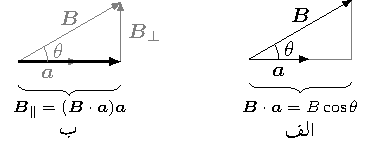
\includegraphics{figVectorComponentAlongUnitVector}
\caption{کسی بھی سمت میں سمتیہ کے جزو کا حصول۔}
\label{شکل_سمتیہ_کسی_سمت_میں_جزو}
\end{figure}
شکل \حوالہ{شکل_سمتیہ_کسی_سمت_میں_جزو}-الف میں سمتیہ \عددیء{\kvec{B}} اور اکائی سمتیہ \عددیء{\kvec{a}}  دکھائے گئے ہیں۔ان کا غیر سمتی ضرب
\begin{align*}
\kvec{B} \cdot \kvec{a} = \abs{\kvec{B}} \abs{\kvec{a}} \cos \theta=B \cos \theta
\end{align*}
کے برابر ہے۔شکل سے واضح ہے کہ یہی \عددیء{\kvec{a}} کی سمت میں \عددیء{\kvec{B}} کے جزو کا طول \عددیء{B_{\parallel}}\حاشیہد{\عددیء{B_{\parallel}} لکھتے ہوئے زیرنوشت میں دو متوازی لکیریں  یہ بتلاتی ہیں کہ \عددیء{\kvec{B}} کا یہ وہ حصہ ہے جو \عددیء{\kvec{a}} کے متوازی ہے۔اسی طرح عمودی مقدار کو عموماً \عددیء{\perp} کی علامت سے ظاہر کیا جاتا ہے۔} ہے۔یوں کسی بھی سمت میں \عددیء{\kvec{B}} کے جزو کا طول حاصل کرنے کی خاطر \عددیء{\kvec{B}} اور اس سمت کی اکائی سمتیہ کا غیر سمتی ضرب حاصل کریں۔یوں حاصل طول کا اکائی سمتیہ کے ساتھ ضرب یعنی \عددیء{(\kvec{B} \cdot \kvec{a}) \kvec{a}} سے اکائی سمتیہ کی سمت میں \عددیء{\kvec{B}} کا سمتی جزو  حاصل ہوتا ہے۔ شکل \حوالہ{شکل_سمتیہ_کسی_سمت_میں_جزو}-ب میں \عددیء{\kvec{a}} کی سمت میں \عددیء{\kvec{B}} کا سمتی جزو \عددیء{\kvec{B}_\parallel} دکھایا گیا ہے۔شکل سے واضح ہے کہ \عددیء{\kvec{B}} سے \عددیء{B_{\parallel} \kvec{a}} منفی کرنے سے  \عددیء{B_\perp} حاصل ہوتا ہے جو \عددیء{\kvec{B}} کا وہ جزو ہے جو \عددیء{\kvec{a}} کے عمودی ہے۔

غیر سمتی ضرب کا حاصل جواب دو صورتوں میں صفر کے برابر ہوتا ہے۔پہلی صورت وہ ہے جب دونوں سمتیوں میں سے کم از کم ایک سمتیہ کا طول صفر کے برابر ہو۔دوسری صورت وہ ہے جب دونوں سمتیات آپس میں عمودی ہوں۔عمودی ہونے کی صورت میں ان کے مابین نوے درجے کا زاویہ ہو گا اور \عددیء{\cos 90=0} کے برابر ہوتا ہے۔یوں دو سمتیوں کے نقطہ ضرب صفر کے برابر ہونے  سے اخذ کیا جاتا ہے کہ یہ آپس میں عمودی ہیں۔ 
%=================

\ابتدا{مثال}
شکل \حوالہ{شکل_سمتیہ_مثال_عمودی_سمتیات_کا_نقطہ_ضرب_صفر} میں تین نقطے \عددیء{M(1,5,6)}، \عددیء{N(4,3,1)} اور \عددیء{P(1,1,4)} دئے گئے ہیں۔\عددیء{M}  اور \عددیء{N} سے گزرتی سیدھی لکیر سے \عددیء{P} کا عمودی فاصلہ حاصل کریں۔ 
\begin{figure}
\centering
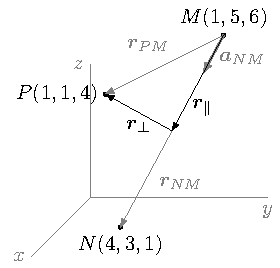
\includegraphics{figVectorExampleOrthognalVectorsHaveZeroDotProdcut}
\caption{متوازی اور عمودی اجزاء۔}
\label{شکل_سمتیہ_مثال_عمودی_سمتیات_کا_نقطہ_ضرب_صفر}
\end{figure}

حل:\عددیء{M} سے \عددیء{N} تک سمتیہ \عددیء{\kvec{r}_{NM}=3\ax-2\ay-5\az} ہے جس کا طول \عددیء{\abs{\kvec{r}_{NM}}=\sqrt{38}} ہے۔یوں اس سمت میں اکائی سمتیہ \عددیء{\kvec{a}_{NM}=\tfrac{3\ax-2\ay-5\az}{\sqrt{38}}} ہو گا۔ اسی طرح \عددیء{M} سے \عددیء{P} تک سمتیہ \عددیء{\kvec{r}_{PM}=-4\ay-2\az} ہے۔\عددیء{\kvec{a}_{NM}} کی سمت میں \عددیء{\kvec{r}_{PM}} کا طول
\begin{align*}
r_{\parallel}=\kvec{r}_{PM} \cdot \kvec{a}_{NM}&=(-4\ay-2\az) \cdot \left(\frac{3\ax-2\ay-5\az}{\sqrt{38}}\right) \\
&=\frac{0+8+10}{\sqrt{38}}=\frac{18}{\sqrt{38}}
\end{align*}
ہے یوں \عددیء{\kvec{a}_{NM}} سمت میں \عددیء{\kvec{r}_{PM}} کا سمتی جزو
\begin{align*}
\kvec{r}_{\parallel}=r_{\parallel} \kvec{a}_{NM}=\frac{18}{38} (3\ax-2\ay-5\az)
\end{align*}
ہے۔\عددیء{\kvec{r}_{PM}} سے \عددیء{\kvec{r}_{\parallel}} منفی کرنے سے لکیر سے \عددیء{P} تک عمودی سمتیہ \عددیء{\kvec{r}_\perp} حاصل ہوتا ہے
\begin{align*}
\kvec{r}_{\perp}=\kvec{r}_{PM}-\kvec{r}_{\parallel}&=(-4\ay-2\az)-\frac{18}{38} (3\ax-2\ay-5\az)\\
&=\frac{-27\ax-58\ay+7\az}{19}
\end{align*}
جس کا طول \عددیء{\tfrac{\sqrt{27^2+58^2+7^2}}{19}=3.3873} ہے۔یوں \عددیء{P} کا لکیر سے عمودی فاصلہ \عددیء{3.3873} ہے۔

\عددیء{\kvec{r}_{\parallel}} اور \عددیء{\kvec{r}_\perp} آپس میں عمودی ہیں لہٰذا ان  کا نقطہ ضرب
\begin{align*}
\kvec{r}_\parallel \cdot \kvec{r}_\perp&=\frac{18}{38} (3\ax-2\ay-5\az) \cdot \left(\frac{-27\ax-58\ay+7\az}{19}\right)=\frac{18}{722}(-81+116-35)=0
\end{align*}
صفر کے برابر ہے۔
\انتہا{مثال}
%===================

شکل \حوالہ{شکل_سمتیہ_مثال_عمودی_سمتیات_کا_نقطہ_ضرب_صفر} میں اگر \عددیء{M} پر \عددیء{\kvec{r}_{NM}} کی دُم رکھی جائے تب  \عددیء{\kvec{r}_{NM}} کی نوک \عددیء{N} کا مقام تعین کرتا ہے۔عموماً کسی بھی نقطے کا مقام محدد کے مرکز \عددیء{(0,0,0)} کی نسبت سے طے کیا جاتا ہے۔ایسا سمتیہ جس کی دُم مرکز پر رکھتے ہوئے اس کی نوک نقطے کا مقام طے کرے  \اصطلاح{مقام تعین کنندہ} سمتیہ\فرہنگ{مقام تعین کنندہ!سمتیہ}\حاشیہب{displacement vector}\فرہنگ{displacement vector} کہلاتا ہے۔اگر تعین کنندہ سمتیہ کو مرکز سے ہٹایا جائے تب ظاہر ہے اس کی نوک اصل مقام طے کرنے سے قاصر ہو گی۔
%=======================================
\ابتدا{مثال}
شکل \حوالہ{شکل_سمتیہ_مثال_عمودی_سمتیات_کا_نقطہ_ضرب_صفر} میں \عددیء{M} سے شروع ہوتے اور  \عددیء{N} جانب بڑھتی سیدھی لکیر پر کسی بھی نقطے کا مقام تعین کرتے تعین کنندہ سمتیہ حاصل کریں۔

حل:مرکز \عددیء{(0,0,0)} سے  نقطہ \عددیء{M} تک کا سمتیہ \عددیء{\kvec{r}_M=1\ax+5\ay+6\az} ہے جبکہ \عددیء{M} سے \عددیء{N} جانب اکائی سمتیہ \عددیء{\kvec{a}_{NM}} گزشتہ مثال میں حاصل کیا گیا۔اکائی سمتیہ \عددیء{\kvec{a}_{NM}} کی سمت میں  \عددیء{M} سے \عددیء{s} فاصلے پر نقطہ \عددیء{Q} تک کا سمتیہ \عددیء{s\kvec{a}_{NM}} ہے۔یوں مرکز سے  \عددیء{Q} تک سمتیہ \عددیء{\kvec{r}_Q=\kvec{r}_M+s\kvec{a}_{NM}} ہو گا۔
\begin{align*}
\kvec{r}_Q=(1\ax+5\ay+6\az) +s \left(\frac{3\ax-2\ay-5\az}{\sqrt{38}}\right)
\end{align*}   
اس مساوات میں \عددیء{s} متغیرہ ہے جسے تبدیل کرتے ہوئے سیدھی لکیر پر کسی بھی نقطہ \عددیء{Q} تک پہنچا جا سکتا ہے۔
\انتہا{مثال}
%==========================
\ابتدا{مثال}
\عددیء{z=z_0} پر \عددیء{1\az} کے عمودی سیدھی سطح کی مساوات حاصل کریں جہاں \عددیء{z_0} مستقل ہے۔ 

حل:نقطہ \عددیء{N_1(0,0,z_0)} سے کسی بھی نقطہ \عددیء{N_2(x,y,z)} تک کا سمتیہ \عددیء{\kvec{r}_{21}=x\ax+y\ay+(z-z_0)\az} ہے۔سطح پر کسی بھی سمتیہ اور سطح کے عمودی سمتیہ آپس میں نوے درجے زاویہ پر پائے جاتے ہیں لہٰذا ان کا غیر سمتی ضرب صفر کے برابر ہو گا۔یوں اگر \عددیء{N_2} اسی عمودی سطح پر پایا جائے تب
\begin{align*}
1\az \cdot [x\ax+y\ay+(z-z_0)\az]=z-z_0=0
\end{align*}
ہو گا جس سے اس سطح کی مساوات \عددیء{z=z_0} حاصل ہوتی ہے۔

اس قیمت کو \عددیء{\kvec{r}_{21}} میں پُر کرتے ہوئے \عددیء{\kvec{r}_{21}=x\ax+y\ay} حاصل ہوتا ہے جہاں \عددیء{x} اور \عددیء{y} آزاد متغیرات ہیں۔چونکہ مرکز سے \عددیء{N_1} کا تعین کنندہ سمتیہ \عددیء{\kvec{r}_{10}=z_0\az} ہے لہٰذا \عددیء{z=z_0} سطح پر کسی بھی نقطہ \عددیء{N_2} کا تعین کنندہ سمتیہ یعنی سطح کی سمتی مساوات  \عددیء{\kvec{r}_{20}=x\ax+y\ay+z_0\az} ہو گی۔
\انتہا{مثال}
%==========
\ابتدا{مشق}
مرکز سے \عددیء{(2,1,3)} تک کی سمتیہ ایک سیدھی سطح کی عمودی سمتیہ ہے۔اس سطح کی  مساوات حاصل کریں۔

جواب:\عددیء{2x+y+3z=14}
\انتہا{مشق}
%============
\حصہ{سمتی ضرب یا صلیبی ضرب}

دو سمتیات \عددیء{\kvec{A}} اور \عددیء{\kvec{B}} کے \اصطلاح{سمتی ضرب}\فرہنگ{سمتی ضرب}\فرہنگ{صلیبی ضرب}\حاشیہب{vector product}\فرہنگ{vector product} کا حاصل جواب سمتیہ ہوتا ہے جس کا طول \عددیء{\kvec{A}} کی مقدار ضربِ  \عددیء{\kvec{B}} کی مقدار ضربِ سمتیوں کے مابین چھوٹے زاویے کے سائن کے برابر ہے۔حاصل سمتیہ \عددیء{\kvec{A}} اور \عددیء{\kvec{B}} سمتیات کی عمودی سمت  میں ہوتا ہے جسے اکائی عمودی سمتیہ \عددیء{\kvec{a}_N} سے ظاہر کیا جائیگا۔
\begin{align}\label{مساوات_سمتیہ_سمتی_ضرب}
\kvec{A} \times \kvec{B}=\abs{\kvec{A}} \abs{\kvec{B}} \sin \theta_{AB} \kvec{a}_N
\end{align}
جس سیدھی سطح پر \عددیء{\kvec{A}} اور \عددیء{\kvec{B}} دونوں پائے جائیں، \عددیء{\kvec{a}_N} اس سطح کے دو عمودی سمتیات میں سے ایک ہے۔\عددیء{\kvec{a}_N} کو \اصطلاح{دائیں ہاتھ کے قانون}\فرہنگ{دائیں ہاتھ!قانون}\حاشیہب{right hand rule}\فرہنگ{right hand rule} سے یوں حاصل کیا جا سکتا ہے۔

\ابتدا{قانون}\شناخت{قانون_سمتیہ_دائیں_ہاتھ_قانون}
دائیں ہاتھ کی ہتھیلی  سیدھی اور انگوٹھے کو بقایا چار انگلیوں کے عمود میں رکھتے ہوئے پہلی انگلی کو \عددیء{\kvec{A}} اور  دوسری انگلی کو \عددیء{\kvec{B}} کی سمت میں رکھیں۔اس صورت میں انگوٹھا \عددیء{\kvec{a}_N} کی سمت میں ہو گا۔  
\انتہا{قانون}

اگر دونوں سمتیات کی دُم ایک ہی جگہ پر نہ ہو تب ان کے مابین زاویہ دریافت کرنے کی  خاطر سمتیوں کی سمت تبدیل کئے بغیر انہیں ایک نقطے پر منتقل کیا جا سکتا ہے۔سمتی ضرب کو سمتیوں کے درمیان صلیبی نشان \عددیء{\times} سے ظاہر کیا جاتا ہے۔اسی وجہ سے اسے \اصطلاح{صلیبی ضرب}\حاشیہب{cross product}\فرہنگ{cross product} بھی کہا جاتا ہے اور \عددیء{\kvec{A} \times \kvec{B}} کو "\عددیء{\kvec{A}} صلیب \عددیء{\kvec{B}}" پڑھا جاتا ہے۔سمتی ضرب میں سمتیوں کی ترتیب نہایت اہم ہے اور انہیں الٹانے سے حاصل جواب کی سمت الٹی ہو جاتی ہے۔
\begin{align}\label{مساوات_سمتیہ_صلیبی_ضرب_ترتیب_الٹاتے_منفی_سمت}
\kvec{A} \times \kvec{B}=- \kvec{B} \times \kvec{A}
\end{align}

اکائی سمتیات \عددیء{\ax} اور \عددیء{\ay} کے مابین نوے درجے کا زاویہ ہے  اور \عددیء{\sin 90\degree=1} کے برابر ہے جبکہ دائیں ہاتھ کے قانون سے ان کے صلیبی ضرب کی سمت \عددیء{\az} حاصل ہوتی ہے۔یوں \عددیء{\ax \times \ay=\az} کے برابر ہے۔اسی طرح \عددیء{\ay \times \az=\ax} اور \عددیء{\az \times \ax=\ay} کے برابر حاصل ہوتے ہیں۔مساوات \حوالہ{مساوات_سمتیہ_صلیبی_ضرب_ترتیب_الٹاتے_منفی_سمت} کے تحت یوں \عددیء{\ay \times \ax=-\az}، \عددیء{\az \times \ay=-\ax} اور \عددیء{\ax \times \az=-\ay} لکھے جا سکتے ہیں۔دو متوازی سمتیوں کے درمیان صفر درجے کا زاویہ ہوتا ہے اور \عددیء{\sin 0 =0} کے برابر ہے لہٰذا \عددیء{\ax \times \ax=0} کے برابر ہے۔اسی طرح \عددیء{\ay \times \ay=0} اور \عددیء{\az \times \az=0} کے برابر ہیں۔ان تمام جوابات کو ایک جگہ لکھتے ہیں۔
\begin{gather}
\begin{aligned}\label{مساوات_سمتیہ_کارتیسی_اکائی_سمتیات_صلیبی_ضرب}
\ax \times \ay &=\az & \ay \times \az&=\ax & \az \times \ax&=\ay\\
\ax \times \ax&=0 & \ay \times \ay&=0 & \az \times \az&=0
\end{aligned}
\end{gather}
%=================

یہی جوابات شکل \حوالہ{شکل_سمتیہ_صلیبی_ضرب_مثبت_دائرہ} کی مدد سے حاصل کئے جا سکتے ہیں۔اس شکل میں گھڑی کی الٹ سمت مثبت سمت ہے۔یوں اگر \عددیء{\ax \times \ay} حاصل کرنا ہو تو شکل میں \عددیء{\ax} سے شروع ہو کر \عددیء{\ay} کی جانب کم راستے پر چلتے ہوئے  \عددیء{\az} حاصل ہوتا ہے۔ساتھ ہی ساتھ چونکہ \عددیء{\ax} سے \عددیء{\ay} جانے کی خاطر  مثبت راستہ اختیار کیا گیا لہٰذا جواب مثبت یعنی \عددیء{+\az} ہو گا۔اس کے برعکس \عددیء{\az \times \ay} حاصل کرنے کی خاطر \عددیء{\az} سے \عددیء{\ay} جانب کم راستے پر چلتے ہوئے \عددیء{\ax} حاصل ہوتا ہے البتہ یہ راستہ گھڑی کے الٹ سمت یعنی منفی سمت میں ہے لہٰذا جواب \عددیء{-\ax} ہو گا۔ 
\begin{figure}
\centering
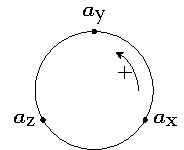
\includegraphics{figVectorCartesianRightHandCircle}
\caption{صلیبی ضرب کا حصول۔}
\label{شکل_سمتیہ_صلیبی_ضرب_مثبت_دائرہ}
\end{figure}

مساوات \حوالہ{مساوات_سمتیہ_کارتیسی_اکائی_سمتیات_صلیبی_ضرب} کی  مدد سے \عددیء{\kvec{A}=A_x\ax+A_y\ay+A_z\az} اور \عددیء{\kvec{B}=B_x\ax+B_y\ay+B_z\az} کی صلیبی ضرب
\begin{align*}
\kvec{A} \times \kvec{B}&=(A_x\ax+A_y\ay+A_z\az) \times (B_x\ax+B_y\ay+B_z\az)\\
&=A_x B_x \ax \times \ax+A_x B_y \ax \times \ay+A_x B_z \ax \times \az\\
& \quad \quad +A_y B_x \ay \times \ax+A_y B_y \ay \times \ay+A_y B_z \ay \times \az \\
&\quad \quad +A_z B_x \az \times \ax+A_z B_y \az \times \ay+A_z B_z \az \times \az
\end{align*}
کو
\begin{align}
\kvec{A} \times \kvec{B}=(A_y B_z-A_z B_y)\ax+(A_z B_x-A_x B_z)\ay+(A_x B_y-A_y B_x)\az
\end{align}
لکھا جا سکتا ہے۔اس جواب کو قالب کے حتمی قیمت کی شکل میں یوں لکھا جا سکتا ہے۔
\begin{align}
\kvec{A} \times \kvec{B}=\begin{vmatrix}
\ax & \ay & \az\\
A_x & A_y & A_z\\
B_x & B_y & B_z
\end{vmatrix}
\end{align}
یوں اگر \عددیء{\kvec{A}=2\ax-3\ay+1\az} اور \عددیء{\kvec{B}=6\ax+5\ay-4\az} ہوں تب
\begin{align*}
\kvec{A} \times \kvec{B}&=\begin{vmatrix*}[r]
\ax & \ay & \az\\
2 & -3 & 1\\
6 & 5 & -4
\end{vmatrix*}\\
&=[(-3)(-4)-(1)(5)]\ax-[(2)(-4)-(1)(6)]\ay+[(2)(5)-(-3)(6)]\az\\
&=7\ax+14\ay+18\az
\end{align*}
ہو گا۔
%===========
\ابتدا{مثال}
\عددیء{N_1(2,3,1)}، \عددیء{N_2(1,6,5)} اور \عددیء{N_3(-2,-3,2)} سیدھی سطح پر پائے جاتے ہیں۔اس سطح کی مساوات حاصل کریں۔

حل:
\begin{align*}
\kvec{r}_{21}&=(1-2)\ax+(6-3)\ay+(5-1)\az=-1\ax+3\ay+4\az\\
\kvec{r}_{31}&=(-2-2)\ax+(-3-3)\ay+(2-1)\az=-4\ax-6\ay+1\az
\end{align*}
کے سمتی ضرب سے ان کا عمودی سمتیہ حاصل ہو گا۔
\begin{align*}
\kvec{r}_N&=(-1\ax+3\ay+4\az) \times (-4\ax-6\ay+1\az)\\
&=6\az+1\ay+12\az+3\ax-16\ay+24\ax\\
&=27\ax-15\ay+18\az
\end{align*}
سطح پر دئے گئے تین نقطوں سے سطح پر کسی بھی نقطہ \عددیء{N_4(x,y,z)} تک کا سمتیہ اس عمودی سمتیہ کے نوے درجے زاویہ پر ہو گا اور یوں ان کا غیر سمتی ضرب صفر کے برابر ہو گا۔\عددیء{N_1} سے \عددیء{N_4} تک سمتیہ \عددیء{\kvec{r}_{41}=(x-2)\ax+(y-3)\ay+(z-1)\az} کے استعمال سے
\begin{align*}
\kvec{r}_{41} \cdot \kvec{r}_{N}=[(x-2)\ax+(y-3)\ay+(z-1)\az] \cdot (27\ax-15\ay+18\az)=0
\end{align*}
لکھ کر
\begin{align*}
27(x-2)-15(y-3)+18(z-1)=0
\end{align*}
سے
\begin{align*}
27x-15y+18z=27
\end{align*}
سیدھی سطح کی مساوات حاصل ہوتی ہے۔ایسی مساوات میں \عددیء{x}، \عددیء{y} اور \عددیء{z} کے مخفف عمودی سمتیہ میں \عددیء{\ax}، \عددیء{\ay} اور \عددیء{\az} کے مخفف \عددیء{27}، \عددیء{-15} اور \عددیء{18} ہوتے ہیں۔

سطح کی مساوات سے \عددیء{z=\tfrac{9-9x+5y}{6}} لکھا جا سکتا ہے۔سطح پر \عددیء{N_4} کی تعین کنندہ مساوات \عددیء{\kvec{r}=x\ax+y\ay+z\az} میں \عددیء{z} کی قیمت پُر کرتے ہوئے  سطح کی سمتی مساوات 
\begin{align*}
\kvec{r}=x\ax+y\ay+\left(\frac{9-9x+5y}{6}\right)\az
\end{align*}
لکھی جا سکتی ہے جہاں \عددیء{x} اور \عددیء{y} آزاد متغیرات ہیں جبکہ \عددیء{z} کو بطور تابع متغیرہ لکھا گیا ہے۔
\انتہا{مثال}
%=========

\ابتدا{مشق}
\عددیء{\kvec{A}=1\ax+3\ay-2\az} اور \عددیء{\kvec{B}=5\ax-2\ay-3\az} کی صورت میں \عددیء{\kvec{A} \times \kvec{B}}، \عددیء{\kvec{B}\times \kvec{A}}، \عددیء{\kvec{A} \times \kvec{A}}، \عددیء{\kvec{a}_B \times \kvec{A}} اور \عددیء{\az \times (\ay \times \kvec{B})} حاصل کریں۔ 
\انتہا{مشق}
%========================

خلاء میں کسی بھی نقطے کا مقام کارتیسی محدد کے علاوہ دیگر طرز کے محدد سے بھی تعین کیا جا سکتا ہے۔ماہرین طبیعیات  تقریباً ایک درجن اقسام کے محددی نظام استعمال کرتے ہیں۔ہم اس کتاب میں کارتیسی نظام کے علاوہ دو مزید اقسام کے محددی نظام استعمال کریں گے۔آئیں انہیں پر غور کریں۔ 

\حصہ{گول نلکی محدد}
کارتیسی نظام میں کسی بھی نقطے کا مقام مرکز سے \عددیء{x}، \عددیء{y} اور \عددیء{z} سمتوں میں فاصلوں سے طے کیا جاتا ہے۔آئیں اب ایسا نظام دیکھیں جس میں ایک عدد زاویہ اور دو عدد فاصلے استعمال کرتے ہوئے کسی بھی نقطے کا مقام طے ہو۔
 \begin{figure}
\centering
\begin{subfigure}{0.5\textwidth}
\centering
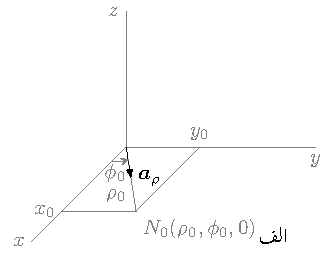
\includegraphics{figVector2and3Dcylindrical}
\end{subfigure}%
%
\begin{subfigure}{0.5\textwidth}
\centering
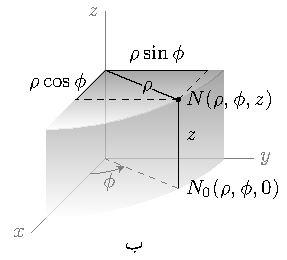
\includegraphics{figVectorCylindricalToCartesian}
\end{subfigure}%
\caption{نلکی محدد}
\label{شکل_سمتیہ_نلکی_محدد}
\end{figure}

شکل \حوالہ{شکل_سمتیہ_نلکی_محدد}-الف میں \عددیء{z=0} سطح پر نقطہ \عددیء{N_0} دکھایا گیا ہے جسے کارتیسی محدد میں \عددیء{N_0(x_0,y_0,0)} لکھا جائے گا۔اگر مرکز سے \عددیء{N_0} تک سیدھی لکیر کی لمبائی \عددیء{\rho_0} اور \عددیء{x} محدد سے اس لکیر کا زاویہ \عددیء{\phi_0} ہو تب اسی نقطے
 کو \اصطلاح{گول نلکی محدد}\فرہنگ{نلکی!محدد}\حاشیہب{cylindrical coordinate system}\فرہنگ{cylindrical!coordinates} کے نظام میں \عددیء{N_0(\rho_0,\phi_0,0)} لکھا جاتا ہے۔اس کتاب میں گول نلکی محدد کا نام چھوٹا کر کے اسے \اصطلاح{نلکی محدد} پکارا جائے گا۔ اگر \عددیء{z=0} سطح پر مرکز سے نقطے کی جانب اکائی سمتیہ \عددیء{\arho} ہو تب مرکز سے نقطے تک سمتیہ کو
\begin{align}
\kvec{\rho}=\rho_0 \arho \quad \quad (\phi=\phi_0, \quad   z=0 )
\end{align}
   لکھا جا سکتا ہے۔نلکی  اور کارتیسی نظام میں  \عددیء{z} محدد یکساں ہیں۔

شکل \حوالہ{شکل_سمتیہ_نلکی_محدد}-الف یا شکل-ب سے کارتیسی اور نلکی محدد کے تعلق اخذ کئے جا سکتے ہیں۔یوں نلکی محدد کے متغیرات \عددیء{(\rho,\phi,z)} سے کارتیسی متغیرات \عددیء{(x,y,z)} یوں حاصل ہوتے ہیں۔
\begin{gather}
\begin{aligned}
x&=\rho \cos \phi\\
y&=\rho \sin \phi\\
z&=z
\end{aligned}
\end{gather}
اسی طرح \عددیء{(x,y,z)} سے  \عددیء{(\rho,\phi,z)} یوں حاصل کئے جاتے ہیں۔
\begin{gather}
\begin{aligned}
\rho&=\sqrt{x^2+y^2} \quad \quad (\rho \ge 0)\\
\phi&=\tan^{-1} \frac{y}{x}\\
z&=z
\end{aligned}
\end{gather}
%
\begin{figure}
\centering
\begin{subfigure}{0.5\textwidth}
\centering
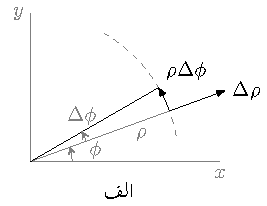
\includegraphics{figVectorCylindricalRadiusAngle}
\end{subfigure}%
%
\begin{subfigure}{0.5\textwidth}
\centering
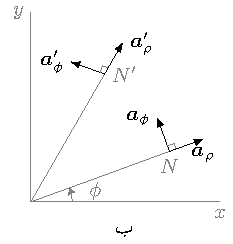
\includegraphics{figVectorCylindricalUnitVectors}
\end{subfigure}%
\caption{نلکی محدد میں متغیرات کے تبدیلی سے فاصلے کا حصول اور اکائی سمتیات۔}
\label{شکل_سمتیہ_نلکی_تبدیلی_متغیرات}
\end{figure}
مندرجہ بالا مساوات میں رداس کی صرف مثبت قیمت لی گئی۔ہم  رداس کی قیمت مثبت ہی لیتے ہیں۔

شکل \حوالہ{شکل_سمتیہ_نلکی_تبدیلی_متغیرات}-الف میں \عددیء{\phi} زاویہ پر \عددیء{\rho} رداس کا ہلکی سیاہی میں دکھایا سمتیہ نقطہ \عددیء{N} ہے۔
اس شکل میں \عددیء{\phi} اور \عددیء{z} تبدیل کئے بغیر \عددیء{\rho} کو \عددیء{\Delta \rho} بڑھتا دکھایا گیا ہے۔اس صورت میں سمتیہ کی نوک \عددیء{\Delta \rho} فاصلہ طے کرتی ہے۔نقطہ \عددیء{N} سے \عددیء{\Delta \rho} کی سمت میں اکائی سمتیہ جسے \عددیء{\arho} لکھا جاتا ہے، نلکی محدد کی  بنیادی اکائی سمتیہ ہے۔اس سمتیہ کو شکل \حوالہ{شکل_سمتیہ_نلکی_تبدیلی_متغیرات}-ب میں دکھایا گیا ہے۔

شکل \حوالہ{شکل_سمتیہ_نلکی_تبدیلی_متغیرات}-الف میں   \عددیء{\rho} اور \عددیء{z} تبدیل کئے بغیر \عددیء{\phi} کو \عددیء{\Delta \phi} بڑھا کر اسی سمتیہ کو گاڑھی سیاہی میں دوبارہ دکھایا گیا ہے۔آپ دیکھ سکتے ہیں کہ  سمتیہ کی نوک نے \عددیء{\rho} رداس کے گول دائرے پر حرکت کرتے ہوئے  \عددیء{\rho \Delta \phi} فاصلہ طے کیا۔یوں اگر زاویہ کو \عددیء{0} تا \عددیء{2\pi} ریڈیئن تبدیل کیا جائے  تو سمتیہ کی نوک گول دائرے پر ایک مکمل چکر کاٹے گی۔جیسے جیسے \عددیء{\Delta \phi} کو کم سے کم کیا جائے ویسے ویسے  \عددیء{\rho \Delta \phi}  گول دائرے کے مماس کی صورت اختیار کرے گی حتٰی کہ \عددیء{\dif \phi} کی صورت میں \عددیء{\rho \dif \phi} گول دائرے کا مماس ہو گا۔نقطہ \عددیء{N} پر بڑھتے \عددیء{\phi} جانب مماس کی سمت میں اکائی سمتیہ کو \عددیء{\aphi} لکھا جاتا ہے۔ اس سمتیہ کو شکل \حوالہ{شکل_سمتیہ_نلکی_تبدیلی_متغیرات}-ب میں دکھایا گیا ہے۔

اسی طرح اگر نقطہ \عددیء{N} پر صرف \عددیء{z} کو \عددیء{\Delta z} تبدیل کیا جائے تب سمتیہ کی نوک \عددیء{\Delta z} فاصلہ طے کرے گی۔ \عددیء{\Delta z} کی سمت میں اکائی سمتیہ جسے \عددیء{\az} لکھا جاتا ہے، نلکی محدد کی تیسری اور آخری بنیادی اکائی سمتیہ ہے۔نلکی محدد کے تین اکائی سمتیات \عددیء{\arho}، \عددیء{\aphi} اور \عددیء{\az} مل کر دائیں ہاتھ کا عمودی  نظام دیتے ہیں۔نقطہ \عددیء{(\rho_1,\phi_1,z_1)} پر نلکی محدد کے اکائی سمتیات کو شکل \حوالہ{شکل_سمتیہ_نلکی_اکائی_سمتیات_عمومی} میں دکھایا گیا ہے۔\عددیء{\arho} گول سطح \عددیء{\rho=\rho_1} کے عمودی ہے۔یہ \عددیء{\phi=\phi_1} اور \عددیء{z=z_1} سطحوں پر پایا جاتا ہے۔اسی طرح \عددیء{\aphi} سیدھی سطح  \عددیء{\phi=\phi_1} کے عمودی ہے۔ یہ \عددیء{z=z_1} سطح پر پایا جاتا ہے اور \عددیء{\rho=\rho_1} نلکی سطح کا مماس ہے۔\عددیء{\az} اکائی سمتیہ \عددیء{z=z_1} سطح کے عمودی ہے۔یہ \عددیء{\rho=\rho_1} اور \عددیء{\phi=\phi_1} سطحوں پر پایا جاتا ہے۔ 
\begin{figure}
\centering
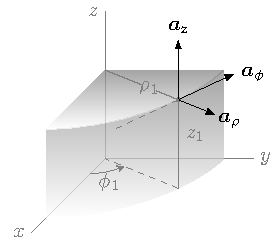
\includegraphics{figVectorCylindricalUnitVectorDirectionsInThreeD}
\caption{نلکی محدد کے اکائی سمتیات۔}
\label{شکل_سمتیہ_نلکی_اکائی_سمتیات_عمومی}
\end{figure}

دائیں ہاتھ کے عمودی نظام میں سمتی ضرب کا حاصل جواب صفحہ \حوالہصفحہ{قانون_سمتیہ_دائیں_ہاتھ_قانون} پر دئے گئے دائیں ہاتھ کے قانون کی مدد سے حاصل کیا جاتا ہے ۔ یوں
\begin{align}
\arho \times \aphi=\az, \quad \aphi \times \az=\arho, \quad \az \times \arho=\aphi
\end{align}
لکھا جا سکتا ہے۔یہی جوابات شکل \حوالہ{شکل_سمتیہ_نلکی_صلیبی_ضرب_مثبت_دائرہ} سے بھی اخذ کئے جا سکتے ہیں۔
\begin{figure}
\centering
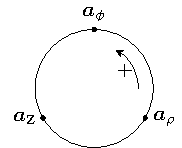
\includegraphics{figVectorCylindricalRightHandCircle}
\caption{صلیبی ضرب کی حاصل اکائی سمتیہ۔}
\label{شکل_سمتیہ_نلکی_صلیبی_ضرب_مثبت_دائرہ}
\end{figure}

کسی سمتیہ کا خود سمتی ضرب صفر کے برابر ہوتا ہے لہٰذا
\begin{align}
\arho \times \arho=0, \quad \aphi \times \aphi =0, \quad \az \times \az=0
\end{align}
لکھا جا سکتا ہے جبکہ کسی بھی اکائی سمتیہ کا خود غیر سمتی ضرب ایک کے برابر ہوتا ہے لہٰذا 
\begin{align}
\arho \cdot \arho=1, \quad \aphi \cdot \aphi =1, \quad \az \cdot \az =1
\end{align}
لکھا جا سکتا ہے۔اسی طرح کسی بھی دو عمودی سمتیات  کا غیر سمتی ضرب صفر کے برابر ہوتا ہے یعنی
\begin{align}
\arho \cdot \aphi=0, \quad \aphi \cdot \az =0, \quad \az \cdot \arho =0
\end{align}

غیر سمتی ضرب کو  \اصطلاح{کرونیکر ڈیلٹا} کی مدد سے یوں لکھا جا سکتا ہے۔
\begin{align}
\kvec{a}_i \cdot \kvec{a}_j=\delta_{ij}
\end{align}
جہاں
\begin{align}
\delta_{ij}=
\begin{cases}
0 \quad  \quad  i\ne j \; \textup{ اگر}\\
1 \quad \quad i=j \; \textup{ اگر}
\end{cases}
\end{align}
کے برابر ہے۔

آپ دیکھتے ہیں کہ کسی بھی نقطہ \عددیء{N(\rho,\phi,z)} پر  اکائی سمتیات حاصل کرنے کی خاطر محدد کے متغیرات \عددیء{\rho}، \عددیء{\phi} اور \عددیء{z} کو  باری باری انتہائی کم بڑھایا جاتا ہے۔جس سمت میں نقطہ حرکت کرے، اسی سمت میں اکائی سمتیہ ہو گی۔شکل \حوالہ{شکل_سمتیہ_نلکی_تبدیلی_متغیرات}-ب میں دو مختلف نقاط \عددیء{N} اور \عددیء{N'} پر نلکی محدد کے عمودی اکائی سمتیات دکھائے گئے ہیں۔آپ دیکھ سکتے ہیں کہ نلکی محدد کے عمودی اکائی سمتیات کی سمت کا دارومدار اس نقطے پر ہے جہاں انہیں حاصل کیا جائے۔آپ جانتے ہیں کہ کارتیسی نظام میں نقطے کا مقام تبدیل کرنے سے کارتیسی اکائی سمتیات تبدیل نہیں ہوتے۔یوں نلکی محدد کے اکائی سمتیات اٹل نہیں ہیں۔یہ ایک انتہائی اہم حقیقت ہے جو تکمل لیتے وقت پیچیدگیاں پیدا کرتا ہے۔تکمل لیتے وقت کارتیسی اکائی سمتیات اٹل ہونے کی بنا پر تکمل کے باہر لے جائے جا سکتے ہیں جبکہ نلکی محدد کے  \عددیء{\arho} اور \عددیء{\aphi} اکائی سمتیات کو تکمل کے باہر نہیں لے جایا جا سکتا۔یاد رہے کہ کسی بھی نقطہ \عددیء{N} پر حاصل کئے گئے \عددیء{\arho}، \عددیء{\aphi} اور \عددیء{\az} آپس میں عمودی ہوں گے جبکہ کسی اور نقطہ \عددیء{N'} پر حاصل کئے گئے \عددیء{\arho'}، \عددیء{\aphi'} اور \عددیء{\az} آپس میں عمودی ہوں گے۔

\جزوحصہ{نلکی اکائی سمتیات کا کارتیسی اکائی سمتیات کے ساتھ غیر سمتی ضرب}
شکل \حوالہ{شکل_سمتیہ_نلکی_کارتیسی_اکائی_غیر_سمتی_ضرب}-الف میں نقطہ \عددیء{N} پر اکائی سمتیات \عددیء{\arho}، \عددیء{\ax} اور \عددیء{\ay} دکھائے گئے ہیں۔\عددیء{\arho} اور  \عددیء{\ax} کے مابین زاویہ \عددیء{\phi} ہے جبکہ اکائی سمتیات کی لمبائی ایک ہوتی ہے لہٰذا
\begin{align}
\arho \cdot \ax=(1)(1)(\cos \phi)=\cos \phi
\end{align}
ہے۔\عددیء{\arho} اور  \عددیء{\ay} کے مابین زاویہ \عددیء{(90^\circ-\phi)} ہے  لہٰذا
\begin{align}
\arho \cdot \ay=(1)(1)[\cos (90^\circ-\phi)]=\sin \phi
\end{align}
کے برابر ہے۔اس مساوات میں \عددیء{\cos(\alpha-\beta)=\cos \alpha \cos \beta+\sin \alpha \sin \beta} کو استعمال کرتے ہوئے \عددیء{\cos(90^\circ-\phi)=\sin \phi} لکھا گیا ہے۔شکل \حوالہ{شکل_سمتیہ_نلکی_کارتیسی_اکائی_غیر_سمتی_ضرب}-ب میں نقطہ \عددیء{N} پر اکائی سمتیات \عددیء{\aphi}، \عددیء{\ax} اور \عددیء{\ay} دکھائے گئے ہیں۔\عددیء{\aphi} اور  \عددیء{\ax} کے مابین زاویہ \عددیء{(90^\circ+\phi)} ہے  لہٰذا
\begin{align}
\aphi \cdot \ax=(1)(1)[\cos (90^\circ+\phi)]=-\sin \phi
\end{align}
ہے۔\عددیء{\aphi} اور  \عددیء{\ay} کے مابین زاویہ \عددیء{\phi} ہے  لہٰذا
\begin{align}
\aphi \cdot \ay=(1)(1)(\cos \phi)=\cos \phi
\end{align}
کے برابر ہے۔\عددیء{\az} کا \عددیء{\ax} اور \عددیء{\ay} کے ساتھ غیر سمتی ضرب صفر کے برابر ہے۔اس کی وجہ ان کے مابین نوے درجے کا زاویہ ہے۔ان تمام غیر سمتی ضرب کو جدول \حوالہ{جدول_سمتیہ_نلکی_کارتیسی_اکائی_غیر-سمتی_ضرب} میں یکجا کیا گیا ہے۔
\begin{figure}
\centering
\begin{subfigure}{0.5\textwidth}
\centering
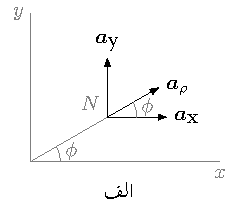
\includegraphics{figVectorCylindricalXandRhoDotProduct}
\end{subfigure}%
%
\begin{subfigure}{0.5\textwidth}
\centering
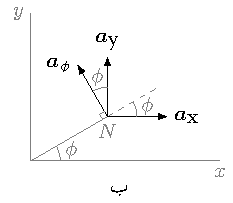
\includegraphics{figVectorCylindricalXandPhiDotProduct}
\end{subfigure}%
\caption{نلکی اکائی سمتیات کا کارتیسی اکائی سمتیات کے ساتھ غیر سمتی ضرب۔}
\label{شکل_سمتیہ_نلکی_کارتیسی_اکائی_غیر_سمتی_ضرب}
\end{figure}%
%
%
\begin{table}
\caption{نلکی اکائی سمتیات کا کارتیسی اکائی سمتیات کے ساتھ غیر سمتی ضرب۔}
\centering
\begin{tabular}{l | r r r}
 & $\ax$ & $\ay$ & $\az$ \\
\hline
$\arho$ & $\cos \phi$ & $\sin \phi $& $0$\\
$\aphi$ &$-\sin \phi$ &$ \cos \phi$ &$ 0$\\
$\az$ & $0$ &$ 0$ &$1$
\end{tabular}
\label{جدول_سمتیہ_نلکی_کارتیسی_اکائی_غیر-سمتی_ضرب}
\end{table}
%
\begin{figure}
\centering
\begin{subfigure}{0.5\textwidth}
\centering
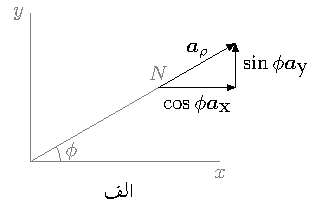
\includegraphics{figVectorCylindricalRhoToCartesianConversion}
\end{subfigure}%
%
\begin{subfigure}{0.5\textwidth}
\centering
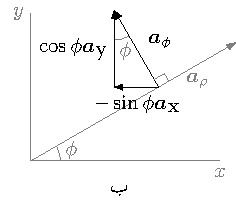
\includegraphics{figVectorCylindricalPhiToCartesianConversion}
\end{subfigure}%
\caption{\عددیء{\arho} اور \عددیء{\aphi} کا کارتیسی نظام میں تبادلہ۔}
\label{شکل_سمتیہ_کارتیسی_نظام_میں_نلکی_رداس_اکائی}
\end{figure}%

\جزوحصہ{نلکی اور کارتیسی اکائی سمتیات کا تعلق}
شکل \حوالہ{شکل_سمتیہ_کارتیسی_نظام_میں_نلکی_رداس_اکائی}-الف میں نقطہ \عددیء{N} پر اکائی سمتیہ \عددیء{\arho} دکھایا گیا ہے۔آپ دیکھ سکتے ہیں کہ کارتیسی محدد میں اسی اکائی سمتیہ کو دو عدد سمتیات کی مدد سے لکھا جا سکتا ہے۔\عددیء{\arho} کی لمبائی ایک کے برابر ہے۔یوں مسئلہ فیثاغورث کی مدد سے
\begin{gather}
\begin{aligned}\label{مساوات_سمتیہ_اکائی_رداس_کارتیسی_میں}
\arho&=\cos \phi \ax+\sin \phi \ay\\
&=\frac{x}{\sqrt{x^2+y^2}} \ax+\frac{y}{\sqrt{x^2+y^2}} \ay
\end{aligned}
\end{gather}
 لکھا جا سکتا ہے جہاں دوسرے قدم پر تمام نلکی محدد کے متغیرات کو کارتیسی متغیرات کی شکل میں لکھا گیا ہے۔شکل \حوالہ{شکل_سمتیہ_کارتیسی_نظام_میں_نلکی_رداس_اکائی}-ب میں نقطہ \عددیء{N} پر اکائی سمتیہ \عددیء{\aphi} دکھایا گیا ہے۔آپ دیکھ سکتے ہیں کہ کارتیسی محدد میں اسی اکائی سمتیہ کو دو عدد سمتیات کی مدد سے یوں  لکھا جا سکتا ہے
\begin{gather}
\begin{aligned}\label{مساوات_سمتیہ_اکائی_زاویہ_کارتیسی_میں}
\aphi&=-\sin \phi \ax+\cos \phi \ay\\
&=-\frac{y}{\sqrt{x^2+y^2}} \ax+\frac{x}{\sqrt{x^2+y^2}} \ay
\end{aligned}
\end{gather}
جہاں دوسرے قدم پر تمام نلکی محدد کے متغیرات کو کارتیسی متغیرات کی شکل میں لکھا گیا ہے۔
%
\begin{figure}
\centering
\begin{subfigure}{0.5\textwidth}
\centering
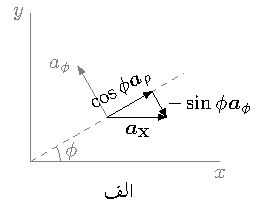
\includegraphics{figVectorCartesianXtoCylindricalConversion}
\end{subfigure}%
%
\begin{subfigure}{0.5\textwidth}
\centering
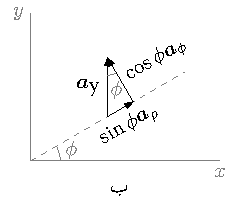
\includegraphics{figVectorCartesianYtoCylindricalConversion}
\end{subfigure}%
\caption{\عددیء{\ax} اور \عددیء{\ay} کا نلکی محدد میں تبادلہ۔}
\label{شکل_سمتیہ_نلکی_محدد_میں_کارتیسی_اکائی_سمتیات}
\end{figure}%

شکل \حوالہ{شکل_سمتیہ_نلکی_محدد_میں_کارتیسی_اکائی_سمتیات}-الف میں \عددیء{\ax} کا نلکی محدد میں تبادلہ دکھایا گیا ہے۔جس نقطے پر ایسا درکار ہو، اس نقطے پر \عددیء{\ax} کی دُم رکھیں۔مرکز سے نقطے تک نقطہ دار سیدھی لکیر کھینچتے ہوئے اسے مزید آگے بڑھائیں۔اس نقطے پر \عددیء{\arho} اسی لکیر کی سمت میں ہو گا جبکہ \عددیء{\aphi} لکیر کے ساتھ نوے درجے کا زاویہ بنائے گا۔شکل میں \عددیء{\aphi} دکھایا گیا ہے۔جیسا شکل میں دکھایا گیا ہے، \عددیء{\ax} کی نوک سے نقطہ دار لکیر پر عمود بنائیں۔صاف ظاہر ہے کہ \عددیء{\ax} کو دو عدد سمتیات کی مدد سے لکھا جا سکتا ہے۔ان میں سے ایک سمتیہ \عددیء{\arho} کی سمت میں اور دوسرا سمتیہ \عددیء{\aphi} کی الٹ جانب کو ہو گا۔یوں
\begin{align}\label{مساوات_سمتیہ_اکائی_ایکس_نلکی_میں}
\ax=\cos \phi \arho-\sin \phi \aphi
\end{align}
لکھا جا سکتا ہے۔شکل \حوالہ{شکل_سمتیہ_نلکی_محدد_میں_کارتیسی_اکائی_سمتیات}-ب میں \عددیء{\ay} کا نلکی محدد میں تبادلہ دکھایا گیا ہے۔یہاں نقطہ پر \عددیء{\ay} کی دُم رکھتے ہوئے اس کی نوک سے نقطہ دار لکیر پر عمود کھینچا گیا ہے۔یوں
\begin{align}\label{مساوات_سمتیہ_اکائی_وائے_نلکی_میں}
\ay=\sin \phi \arho+\cos \phi \aphi
\end{align}
لکھا جا سکتا ہے۔

آئیں مساوات \حوالہ{مساوات_سمتیہ_اکائی_رداس_کارتیسی_میں} تا مساوات \حوالہ{مساوات_سمتیہ_اکائی_وائے_نلکی_میں} کو جدول \حوالہ{جدول_سمتیہ_نلکی_کارتیسی_اکائی_غیر-سمتی_ضرب} کی مدد سے حاصل کریں۔کسی بھی سمتیہ \عددیء{\kvec{A}} کو کارتیسی یا نلکی محدد میں لکھا جا سکتا ہے۔یوں
\begin{gather}
\begin{aligned}\label{مساوات_سمتیہ_سمتیہ_نلکی_کارتیسی_اشکال}
\kvec{A}&=A_x \ax+A_y \ay+A_z\az\\
&=A_\rho \arho+A_\phi \aphi+A_z \az
\end{aligned}
\end{gather}
لکھا جا سکتا ہے۔ان میں پہلی مساوات کا باری باری \عددیء{\ax}، \عددیء{\ay} اور \عددیء{\az} کے ساتھ غیر سمتی ضرب لیتے ہوئے 
\begin{gather}
\begin{aligned}\label{مساوات_سمتیہ_کارتیسی_اجزاء}
\ax \cdot \kvec{A}&=A_x \ax \cdot \ax+A_y \ax \cdot \ay+A_z \ax \cdot \az=A_x\\
\ay \cdot \kvec{A}&=A_x \ay \cdot \ax+A_y \ay \cdot \ay+A_z \ay \cdot \az=A_y\\
\az \cdot \kvec{A}&=A_x \az \cdot \ax+A_y \az \cdot \ay+A_z \az \cdot \az=A_z
\end{aligned}
\end{gather}
حاصل ہوتے ہیں۔\عددیء{\kvec{A}} کو کارتیسی نظام میں لکھنے کی خاطر \عددیء{A_x}، \عددیء{A_y} اور \عددیء{A_z} درکار ہوتے ہیں جنہیں مندرجہ بالا مساوات سے حاصل کیا جا سکتا ہے۔اسی طرح مساوات \حوالہ{مساوات_سمتیہ_سمتیہ_نلکی_کارتیسی_اشکال} کے نچلے حصے کا باری باری \عددیء{\arho}، \عددیء{\aphi} اور \عددیء{\az} کے ساتھ غیر سمتی ضرب لیتے ہوئے
\begin{gather}
\begin{aligned}\label{مساوات_سمتیہ_نلکی_اجزاء}
\arho \cdot \kvec{A}&=A_\rho \arho \cdot \arho +A_\phi \arho \cdot \aphi +A_z \arho \cdot \az=A_\rho\\
\aphi \cdot \kvec{A}&=A_\rho \aphi \cdot \arho +A_\phi \aphi \cdot \aphi +A_z \aphi \cdot \az=A_\phi \\
\az \cdot \kvec{A}&=A_\rho \az \cdot \arho +A_\phi \az \cdot \aphi +A_z \az \cdot \az=A_z
\end{aligned}
\end{gather}
حاصل ہوتے ہیں۔یوں \عددیء{\kvec{A}} کو نلکی نظام میں لکھنے کی خاطر \عددیء{A_\rho}، \عددیء{A_\phi} اور \عددیء{A_z} کو مندرجہ بالا مساوات کی مدد سے حاصل کیا جا سکتا ہے۔

آئیں \عددیء{\arho} کو کارتیسی نظام میں لکھیں۔یوں \عددیء{\kvec{A}=\arho} کو  کارتیسی نظام میں لکھنا مطلوب ہے۔مساوات \حوالہ{مساوات_سمتیہ_کارتیسی_اجزاء} کے مطابق  \عددیء{A_x} حاصل کرنے کی خاطر \عددیء{\ax \cdot \kvec{A}} لینا ہو گا۔جدول \حوالہ{جدول_سمتیہ_نلکی_کارتیسی_اکائی_غیر-سمتی_ضرب} کے استعمال سے
\begin{align*}
A_x=\ax \cdot \kvec{A}=\ax \cdot \arho=\cos \phi
\end{align*}  
حاصل ہوتا ہے۔اسی طرح جدول کو استعمال کرتے ہوئے
\begin{align*}
A_y=\ay \cdot \kvec{A}=\ay \cdot \arho=\sin \phi
\end{align*}
اور 
\begin{align*}
A_z=\az \cdot \kvec{A}=\az \cdot \arho=0
\end{align*}
حاصل کرتے  ہیں۔یوں کارتیسی نظام میں \عددیء{\kvec{A}=A_x\ax+A_y\ay+A_z\az} لکھتے ہوئے
\begin{align*}
\arho = \cos \phi \ax +\sin \phi \ay
\end{align*}
لکھا جائے گا۔ یہی جواب مساوات \حوالہ{مساوات_سمتیہ_اکائی_رداس_کارتیسی_میں} میں بھی حاصل کیا گیا تھا۔

\عددیء{\aphi} کو بھی اسی طرح کارتیسی نظام میں لکھا جا سکتا ہے۔ایسا کرنے کی خاطر جدول \حوالہ{جدول_سمتیہ_نلکی_کارتیسی_اکائی_غیر-سمتی_ضرب} کی مدد سے  اس سمتیہ کا باری باری \عددیء{\ax}، \عددیء{\ay} اور \عددیء{\az} کے ساتھ غیر سمتی ضرب لیتے ہیں۔
\begin{align*}
A_x&=\ax \cdot \aphi=-\sin \phi\\
A_y&=\ay \cdot \aphi=\cos \phi\\
A_z&=\az \cdot \aphi=0
\end{align*}
یوں
\begin{align*}
\aphi=A_x \ax+A_y \ay+A_z \az = -\sin \phi \ax+\cos \phi \ay
\end{align*}
حاصل ہوتا ہے۔یہی جواب مساوات \حوالہ{مساوات_سمتیہ_اکائی_زاویہ_کارتیسی_میں} بھی دیتا ہے۔

آپ سے گزارش ہے کہ جدول \حوالہ{مساوات_سمتیہ_اکائی_زاویہ_کارتیسی_میں} کو یاد کرنے کی کوشش نہ کریں۔اپنے آپ میں یہ صلاحیت پیدا کریں کہ ان جوابات کو آپ جلد اخذ کر سکیں۔

\ابتدا{مشق}
\عددیء{\ax}، \عددیء{\ay} اور \عددیء{\az} کو جدول \حوالہ{جدول_سمتیہ_نلکی_کارتیسی_اکائی_غیر-سمتی_ضرب} کی مدد سے  نلکی محدد میں لکھیں۔
\انتہا{مشق}
%
\begin{figure}
\centering
\begin{subfigure}{0.5\textwidth}
\centering
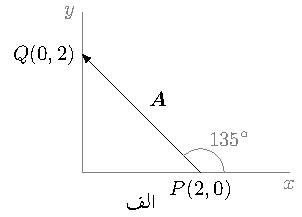
\includegraphics{figVectorVectorInCartesianAndCylindricalA}
\end{subfigure}%
%
\begin{subfigure}{0.5\textwidth}
\centering
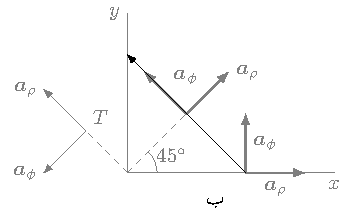
\includegraphics{figVectorVectorInCartesianAndCylindricalB}
\end{subfigure}%
\caption{کارتیسی اور نلکی محدد میں سمتیہ۔}
\label{شکل_سمتیہ_کارتیسی_نلکی_مساوات}
\end{figure}

شکل \حوالہ{شکل_سمتیہ_کارتیسی_نلکی_مساوات} میں \عددیء{P(2,0)} سے \عددیء{Q(0,2)} تک سمتیہ \عددیء{\kvec{A}} دکھایا گیا ہے۔کارتیسی نظام میں 
\begin{align}\label{مساوات_سمتیہ_کارتیسی_نظام_سمتیہ_مثال}
\kvec{A}&=-2\ax+2\ay
\end{align}
لکھا جا سکتا ہے۔اس سمتیہ کی حتمی قیمت
\begin{align*}
\abs{\kvec{A}}= \sqrt{\kvec{A} \cdot \kvec{A}}=\sqrt{(-2\ax+2\ay) \cdot (-2\ax+2\ay)}=\sqrt{8}
\end{align*}
ہے۔آئیں اسی سمتیہ کو نلکی محدد میں لکھیں۔ایسا کرنے کی خاطر \عددیء{A_\rho} اور \عددیء{A_\phi} درکار ہوں گے جنہیں حاصل کرنے کی خاطر جدول \حوالہ{جدول_سمتیہ_نلکی_کارتیسی_اکائی_غیر-سمتی_ضرب}  کی مدد سے \عددیء{\arho \cdot \kvec{A}} اور \عددیء{\aphi \cdot \kvec{A}} حاصل کرتے ہیں۔
\begin{align*}
A_\rho&=\arho \cdot (-2\ax+2\ay)=-2 \cos \phi +2 \sin \phi\\
A_\phi&=\aphi \cdot  (-2\ax+2\ay)=2 \sin \phi +2 \cos \phi
\end{align*}
یوں
\begin{align}\label{مساوات_سمتیہ_نلکی_نظام_سمتیہ_مثال}
\kvec{A}=2(- \cos \phi + \sin \phi) \arho +2( \sin \phi + \cos \phi)\aphi
\end{align}
لکھا جا سکتا ہے۔آئیں دیکھیں کہ اس کی حتمی قیمت کیا حاصل ہوتی ہے۔اکائی سمتیات کا غیر سمتی ضرب \عددیء{\arho \cdot \arho=1}، \عددیء{\aphi \cdot \aphi=1} اور \عددیء{\arho \cdot \aphi=0} استعمال کرتے ہوئے
\begin{align*}
\abs{\kvec{A}}&=\sqrt{\kvec{A} \cdot \kvec{A}}\\
&=\sqrt{2^2(- \cos \phi + \sin \phi)^2+2^2( \sin \phi + \cos \phi)^2 }\\
&=\sqrt{4(\cos^2 \phi +\sin^2 \phi -2 \cos \phi \sin \phi)+4(\cos^2 \phi +\sin^2 \phi +2 \cos \phi \sin \phi)}\\
&=\sqrt{8(\cos^2 \phi+\sin^2 \phi)}\\
&=\sqrt{8}
\end{align*}
حاصل ہوتا ہے جہاں آخری قدم پر \عددیء{\cos^2 \alpha+\sin^2 \alpha=1} کا استعمال کیا گیا ہے۔یقیناً سمتیہ کی حتمی قیمت محدد کے نظام پر منحصر نہیں۔

مساوات \حوالہ{مساوات_سمتیہ_کارتیسی_نظام_سمتیہ_مثال} اور مساوات \حوالہ{مساوات_سمتیہ_نلکی_نظام_سمتیہ_مثال} ایک ہی سمتیہ کو لکھنے کے دو طریقے ہیں۔یہاں کارتیسی نظام کا استعمال نہایت آسان ثابت ہوا۔ آگے چل کر آپ دیکھیں گے کہ کہیں مسئلوں میں نلکی محدد کا استعمال زیادہ آسان ہو گا۔آئیں مساوات \حوالہ{مساوات_سمتیہ_کارتیسی_نظام_سمتیہ_مثال} پر مزید غور کریں۔اس مساوات میں اکائی سمتیات از خود اٹل نہیں ہیں۔ان کی سمتوں کا دارومدار زاویہ \عددیء{\phi} پر ہے۔شکل  \حوالہ{شکل_سمتیہ_کارتیسی_نلکی_مساوات}-ب میں \عددیء{\phi=0^\circ}، \عددیء{\phi=45^\circ} اور \عددیء{\phi=135^\circ} پر \عددیء{\arho} اور \عددیء{\aphi} دکھائے گئے ہیں۔نقطہ \عددیء{P} یعنی \عددیء{\phi=0^\circ} پر مساوات \حوالہ{مساوات_سمتیہ_نلکی_نظام_سمتیہ_مثال} 
\begin{align*}
\kvec{A}_{ \phi=0^\circ}&=2(- \cos 0^\circ + \sin 0^\circ ) \arho +2( \sin 0^\circ  + \cos 0^\circ )\aphi\\
&=-2\arho+2\aphi 
\end{align*} 
صورت اختیار کر لیتی ہے۔اس مساوات کے مطابق \عددیء{\phi=0^\circ} پر \عددیء{\kvec{A}} کو دو عدد سمتیات کے مجموعہ کی صورت میں لکھا جا سکتا ہے جن میں پہلی سمتیہ \عددیء{\arho} کے الٹ سمت میں ہے اور اس کی لمبائی دو کے برابر ہے جبکہ دوسری سمتیہ کی مقدار دو اور اس کی سمت \عددیء{\aphi} کی سمت میں ہی ہے۔\حوالہ{شکل_سمتیہ_کارتیسی_نلکی_مساوات}-ب میں نقطہ \عددیء{P} پر \عددیء{\kvec{A}} کی سمت واقع بڑھتی \عددیء{\aphi} اور گھٹتی \عددیء{\arho} کی سمت میں ہے۔یاد رہے کہ اس مساوات میں \عددیء{\arho} اور \عددیء{\aphi} کو \عددیء{\phi=0^\circ} پر حاصل کیا گیا ہے۔\عددیء{\phi=0^\circ} پر \عددیء{\arho} اور \عددیء{\ax} برابر ہوتے ہیں اور اسی طرح \عددیء{\aphi} اور \عددیء{\ay} برابر ہوتے ہیں۔یہی وجہ ہے کہ مساوات \حوالہ{مساوات_سمتیہ_کارتیسی_نظام_سمتیہ_مثال} میں \عددیء{\ax} کی جگہ \عددیء{\arho} اور \عددیء{\ay} کی جگہ \عددیء{\aphi} پُر کرنے سے مندرجہ بالا مساوات لکھی جا سکتی ہے۔

\عددیء{\phi=45^\circ} پر مساوات \حوالہ{مساوات_سمتیہ_نلکی_نظام_سمتیہ_مثال}
\begin{align*}
\kvec{A}_{\phi=45^\circ}&=2(- \cos 45^\circ + \sin 45^\circ ) \arho +2( \sin 45^\circ  + \cos 45^\circ )\aphi\\
&=2(- \frac{1}{\sqrt{2}} +\frac{1}{\sqrt{2}} ) \arho +2( \frac{1}{\sqrt{2}}  + \frac{1}{\sqrt{2}} )\aphi\\
&=\sqrt{8} \aphi
\end{align*} 
صورت اختیار کر لیتی ہے۔اس مساوات کے مطابق \عددیء{\phi=45^\circ} پر \عددیء{\kvec{A}} صرف اور صرف \عددیء{\aphi} کی سمت میں ہے اور اس کی لمبائی \عددیء{\sqrt{8}} ہے۔شکل \حوالہ{شکل_سمتیہ_کارتیسی_نلکی_مساوات}-ب میں یہ حقیقت واضح ہے کہ \عددیء{\phi=45^\circ}  پر \عددیء{\kvec{A}} کی سمت \عددیء{\aphi} ہی ہے۔یاد رہے کہ اس مساوات میں \عددیء{\arho} اور \عددیء{\aphi} کو \عددیء{\phi=45^\circ} پر حاصل کیا گیا ہے۔شکل میں اکائی سمتیات کو عین \عددیء{\kvec{A}} کے اوپر کھینچا گیا ہے تا کہ سمتیات کی سمتوں کا موازنہ آسانی سے کیا جا سکے۔

آپ نے دیکھا کہ نلکی محدد میں سمتیہ کی مساوات کا دارومدار اس نقطے پر ہے جس نقطے کے اکائی سمتیات استعمال کئے جائیں۔آئیں دیکھیں کہ \عددیء{\phi=135^\circ} پر پائے جانے والے  نقطہ \عددیء{T} کے اکائی سمتیات استعمال کرتے ہوئے \عددیء{\kvec{A}} کیسا لکھا جائے گا۔مساوات \حوالہ{مساوات_سمتیہ_نلکی_نظام_سمتیہ_مثال} میں \عددیء{\phi=135^\circ} پُر کرنے سے
\begin{align*}
\kvec{A}_{\phi=135^\circ}&=2(- \cos 135^\circ + \sin 135^\circ) \arho +2( \sin 135^\circ + \cos 135^\circ)\aphi\\
&=2(\frac{1}{\sqrt{2}}+\frac{1}{\sqrt{2}})\arho+2(\frac{1}{\sqrt{2}}-\frac{1}{\sqrt{2}})\aphi\\
&=\sqrt{8}\arho
\end{align*}
حاصل ہوتا ہے۔اس مساوات کے مطابق \عددیء{\phi=135^\circ} کے اکائی سمتیات استعمال کرتے ہوئے \عددیء{\kvec{A}} کو \عددیء{\arho} کی سمت میں \عددیء{\sqrt{8}} لمبائی کا سمتیہ لکھا جا سکتا ہے۔شکل سے یہ حقیقت واضح ہے۔ 
%
\begin{figure}
\centering
\begin{subfigure}{0.5\textwidth}
\centering
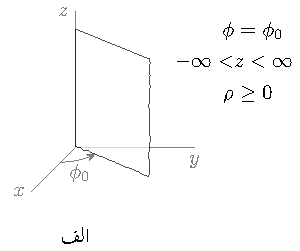
\includegraphics{figVectorCylindricalFixedAngleSurface}
\end{subfigure}%
%
\begin{subfigure}{0.5\textwidth}
\centering
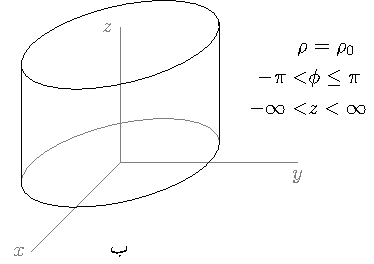
\includegraphics{figVectorCylindricalFixedRadiusSurface}
\end{subfigure}%
\caption{$\phi=\phi_0$ اور $\rho=\rho_0$ سطحیں۔}
\label{شکل_سمتیہ_نلکی_قطعی_زاویہ_سطح}
\end{figure}
\جزوحصہ{نلکی لامحدود سطحیں}
شکل \حوالہ{شکل_سمتیہ_نلکی_قطعی_زاویہ_سطح}-الف میں \عددیء{\phi} تبدیل کئے بغیر \عددیء{\rho} اور \عددیء{z} کی قیمتیں تبدیل کرتے ہوئے \عددیء{\phi=\phi_0} سطح کا حصول دکھایا گیا ہے۔یہ سطح نلکی شکل رکھتی ہے  جس کا اوپر والا منہ اور نچلا منہ کھلے ہیں یعنی ان پر ڈھکن نہیں۔شکل-ب میں \عددیء{\rho} تبدیل کئے بغیر \عددیء{\phi} اور \عددیء{z} کو تبدیل کرتے ہوئے \عددیء{\rho=\rho_0} سطح کا حصول دکھایا گیا ہے۔ان دونوں لامحدود سطحوں کے کچھ حصے ان  اشکال میں  دکھائے گئے ہیں۔ شکل-الف میں \عددیء{\rho} کی قیمت صرف مثبت جبکہ \عددیء{z} کی قیمت مثبت یا منفی ممکن ہے۔شکل-ب میں زاویہ کُل \عددیء{2\pi} ریڈیئن تبدیل ہو سکتا ہے۔یوں زاویے کا مثبت حد \عددیء{\pi} ریڈیئن یعنی \عددیء{180} درجہ ہے جبکہ اس کا منفی\حاشیہد{حقیقت میں منفی حد \عددیء{-180^\circ} کو نہیں چھوتا۔اگر منفی حد \عددیء{-180^\circ} کو چھوئے تب منفی \عددیء{x} محدد دو مرتبہ شامل ہوتا ہے۔} حد \عددیء{-\pi} یعنی \عددیء{-180} درجے ہے۔نلکی محدد اور کارتیسی نظام دونوں میں \عددیء{z=z_0}  سطح یکساں بنتی ہے۔

جیسے شکل \حوالہ{شکل_سمتیہ_نلکی_تین_سطحیں} میں دکھایا گیا ہے، \عددیء{\rho=\rho_1} اور \عددیء{\phi=\phi_1}  سطحیں \عددیء{\az} کی سیدھ میں سیدھی لکیر پر ملتے ہیں۔اسی طرح \عددیء{\rho=\rho_1} اور \عددیء{z=z_1} سطحیں ایک گول دائرے پر ملتے ہیں جبکہ \عددیء{\phi=\phi_1} اور \عددیء{z=z_1} سطحیں \عددیء{\arho} کی سیدھ میں سیدھی لکیر پر ملتے ہیں۔\عددیء{\rho=\rho_1}، \عددیء{\phi=\phi_1} اور \عددیء{z=z_1} سطحیں صرف اور صرف ایک ہی نقطہ \عددیء{N} پر اکٹھے ملتے ہیں۔نلکی محدد میں کسی بھی نقطے  کا مقام اسی طرح تین سطحوں کے  متقاطع نقطہ سے حاصل کیا جاتا ہے البتہ \عددیء{(0,0,z)} تک پہنچنے کی خاطر ایسا کرنے کی ضرورت نہیں ہوتی۔

\begin{figure}
\centering
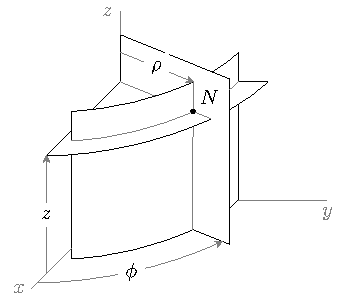
\includegraphics{figVectorCylindricalIntersectingSurfaces}
\caption{نلکی محدد کے تین سطحیں۔}
\label{شکل_سمتیہ_نلکی_تین_سطحیں}
\end{figure}
کسی بھی نقطہ \عددیء{N(\rho_1,\phi_1,z_1)} پر \عددیء{\rho=\rho_1}، \عددیء{\phi=\phi_1} اور \عددیء{z=z_1} سطحیں  بنانے کے بعد اگر نلکی محدد کے متغیرات کو \عددیء{\dif \rho}، \عددیء{\dif \phi} اور \عددیء{\dif z} بڑھا کر مزید تین سطحیں کھینچے جائیں تو یہ چھ سطحیں مل کر منحرف مکعب کو گھیریں گے جسے شکل \حوالہ{شکل_سمتیہ_نلکی_چھوٹی_حجم}-الف میں دکھایا گیا ہے۔رداسی سمت میں اس منحرف مکعب کے اطراف کی لمبائی \عددیء{\dif \rho} جبکہ \عددیء{\az}  سمت کے اطراف کی لمبائی \عددیء{\dif z} ہے۔ \عددیء{\aphi} سمت میں \عددیء{z} محدد کے قریبی  گول طرف کی لمبائی \عددیء{\rho \dif \phi} جبکہ محدد سے دور طرف کی گول لمبائی \عددیء{(\rho+\dif \rho)\dif \phi} ہے۔جیسے جیسے اس منحرف مکعب کو چھوٹا کیا جائے ویسے ویسے یہ ایک درست مکعب کی صورت اختیار کرتا ہے لہٰذا نہایت چھوٹے حجم کو مکعب تصور کرتے ہوئے اس کا حجم \عددیء{\rho \dif \rho \dif \phi \dif z} لکھا جا سکتا ہے۔
\begin{figure}
\centering
\begin{subfigure}{0.5\textwidth}
\centering
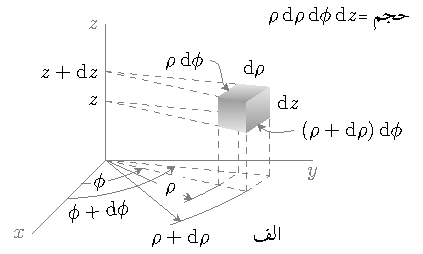
\includegraphics{figVectorCylindricalDifferentialVolume}
\end{subfigure}%
%
\begin{subfigure}{0.5\textwidth}
\centering
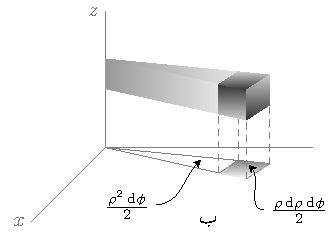
\includegraphics{figVectorCylindricalDifferentialTrapezium}
\end{subfigure}%
\caption{نلکی محدد میں انتہائی چھوٹی حجم۔}
\label{شکل_سمتیہ_نلکی_چھوٹی_حجم}
\end{figure}  

شکل \حوالہ{شکل_سمتیہ_نلکی_چھوٹی_حجم}-ب میں چھوٹے منحرف مکعب کو رداسی سمت میں \عددیء{z} محدد تک بڑھا کر پچر یا فانہ کی شکل میں دکھایا گیا ہے۔\عددیء{z=0} سطح پر اس کا عمودی سایہ بھی دکھایا گیا ہے۔\عددیء{\rho} رداس کے گول دائرے  کے مرکز سے  \عددیء{\dif \phi} زاویے پر دو لکیریں دائرے تک کھینچنے سے  \عددیء{\tfrac{\rho^2 \dif \phi}{2}} رقبہ گھیرا جاتا ہے۔اگر رداس \عددیء{\rho+\dif \rho} ہو تب رقبہ \عددیء{\tfrac{(\rho+\dif \rho)^2 \dif \phi}{2}} ہو گا۔یوں شکل-ب میں چھوٹے مکعب کے سایہ  کا رقبہ \عددیء{\dif S}
\begin{align*}
\dif S&=\frac{(\rho+\dif \rho)^2 \dif \phi}{2} - \frac{\rho^2 \dif \phi}{2}\\
&=\frac{\rho^2 \dif \phi +2 \rho \dif \rho \dif \phi+(\dif \rho)^2 \dif \phi}{2}-\frac{\rho^2 \dif \phi}{2}\\
&=\rho \dif \rho \dif \phi+\frac{(\dif \rho)^2 \dif \phi}{2}\\
&\approx \rho \dif \rho \dif \phi
\end{align*}
ہو گا۔یہاں آخری قدم پر \عددیء{\dif} کی علامت، مجموعہ کے پہلے رکن میں دو مرتبہ  جبکہ دوسرے رکن میں تین مرتبہ ہے۔یوں دوسرے اور پہلے رکن کی نسبت
  \عددیء{\tfrac{0.5(\dif \rho)^2 \dif \phi}{\rho \dif \rho \dif \phi}=\tfrac{\dif \rho}{2\rho}} ہو گی۔\عددیء{\dif \rho} کو کم سے کم\حاشیہد{کسی بھی متغیرہ مثلاً \عددیء{\rho} میں چھوٹی سی تبدیلی کو \عددیء{\Delta \rho} لکھا جاتا ہے جبکہ اس میں کم سے کم تبدیلی کو \عددیء{\dif \rho} لکھا 
جاتا ہے۔\عددیء{\dif \rho} کو تقریباً صفر سمجھا جا سکتا ہے یعنی \عددیء{\dif \rho \to 0} ہوتا ہے۔} کرتے ہوئے دوسرے رکن کو قابل نظر انداز بناتے ہوئے نظرانداز کیا گیا ہے۔یوں \عددیء{\rho \dif \rho \dif \phi} رقبہ اور \عددیء{\dif z} بلندی کے مکعب کا حجم \عددیء{\rho \dif \rho \dif \phi \dif z} ہو گا۔

شکل \حوالہ{شکل_سمتیہ_نلکی_چھوٹی_حجم} کو درست مکعب تصور کرتے ہوئے، اس کے اطراف کی لمبائی \عددیء{\rho \dif \phi}، \عددیء{\dif \rho} اور \عددیء{\dif z} لی جاتی ہے۔یوں مکعب کے نچلی اور اوپر سطح کا رقبہ مستطیل کے اطراف کو ضرب دیتے ہوئے  \عددیء{\rho \dif \rho \dif \phi} لکھا جا سکتا ہے۔اسی طرح سامنے اور پیچھے سطحوں  کا رقبہ \عددیء{\dif \rho \dif z} جبکہ بائیں اور دائیں سطحوں کا رقبہ \عددیء{\rho \dif \phi \dif z} لکھا جا سکتا ہے۔

\حصہ{کروی محدد}
سیدھی لکیروں اور سیدھی سطحوں کو کارتیسی محدد میں زیادہ آسانی سے ظاہر کیا جا سکتا ہے جبکہ نلکی سطحوں کو ظاہر کرنے کے لئے نلکی محدد بہتر ثابت ہوتا ہے۔اسی طرح کرہ اشکال کے سطحوں کو کروی محدد میں باآسانی لکھا جا سکتا ہے۔آئیں کروی نظام پر غور کریں۔

شکل \حوالہ{شکل_سمتیہ_کروی_محدد_متغیرات}-الف میں کروی محدد کے متغیرات \عددیء{r}، \عددیء{\theta} اور \عددیء{\phi} دکھائے گئے ہیں۔محدد کے مرکز سے نقطہ \عددیء{N} تک کے فاصلے \عددیء{r} کو کروی رداس پکارا جاتا ہے جبکہ \عددیء{z} محدد سے کروی رداس تک زاویے کو \عددیء{\theta} لکھا جاتا ہے۔\عددیء{x} محدد سے رداس کے عمودی سائے تک زاویہ \عددیء{\phi} ہے۔کروی اور نلکی نظام میں \عددیء{\phi} یکساں بیان کیا جاتا ہے۔رداس کی  قیمت مثبت لی جاتی ہے۔یوں \عددیء{r \ge 0} ممکن ہے۔\عددیء{\theta} کی کم سے کم قیمت \عددیء{0^\circ} اور  زیادہ سے زیادہ  قیمت \عددیء{180^\circ} ہے جبکہ \عددیء{\phi} کی کم سے کم قیمت \عددیء{0^\circ} اور زیادہ سے زیادہ قیمت \عددیء{360^\circ} ہے۔

\begin{figure}
\centering
\begin{subfigure}{0.5\textwidth}
\centering
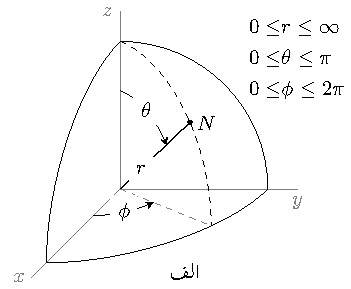
\includegraphics{figVectorSphericalRadiusThetaPhi}
\end{subfigure}%
%
\begin{subfigure}{0.5\textwidth}
\centering
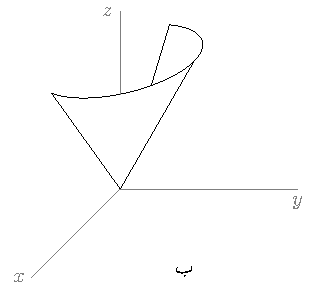
\includegraphics{figVectorSphericalThetaSurface}
\end{subfigure}%
\caption{{الف} کروی محدد کے متغیرات۔ {ب} \عددیء{\theta=\theta_0} سطح  کا کچھ حصہ۔}
\label{شکل_سمتیہ_کروی_محدد_متغیرات}
\end{figure}
%
\عددیء{r} اور \عددیء{\phi} تبدیل کئے بغیر \عددیء{\theta} کو \عددیء{0} سے بڑھاتے ہوئے \عددیء{\pi} ریڈیئن  کرنے سے نقطہ \عددیء{N}  شکل \حوالہ{شکل_سمتیہ_کروی_محدد_متغیرات}-الف میں نقطہ دار لکیر پر چلتے ہوئے  مثبت \عددیء{z} محدد سے شروع ہو کر  منفی \عددیء{z} محدد پر پہنچتا ہے۔اسے  نقطہ دار لکیر کو  کرہ ارض کے \اصطلاح{خط طول بلد}\فرہنگ{خط!طول بلد}\حاشیہب{longitude}\فرہنگ{longitude} تصور  کیا جا سکتا ہے۔  شکل-الف میں \عددیء{\theta} کا \عددیء{0^\circ} تا \عددیء{90^\circ} تبدیل ہوتا دکھایا گیا ہے۔اسی طرح \عددیء{r} اور \عددیء{\theta} تبدیل کئے بغیر \عددیء{\phi} کو \عددیء{0^\circ} تا \عددیء{360^\circ} تبدیل کرنے سے  نقطہ \عددیء{N} گول دائرے پر \عددیء{z} محدد کے گرد ایک چکر کاٹے گا۔یہ حرکت کرہ ارض کے \اصطلاح{خط عرض بلد}\فرہنگ{خط!عرض بلد}\حاشیہب{latitude}\فرہنگ{latitude} پر چلنے کے  مانند ہے۔\عددیء{\theta} اور \عددیء{\phi} تبدیل کئے بغیر \عددیء{r} کو تبدیل کرنے سے نقطہ \عددیء{N} مرکز سے  سیدھی باہر نکلتی لکیر پر حرکت کرتا ہے۔ 

\begin{figure}
\centering
\begin{subfigure}{0.5\textwidth}
\centering
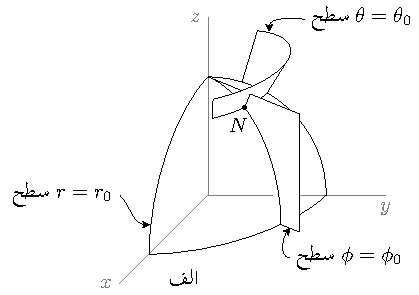
\includegraphics{figVectorSphericalIntersectingSurface}
\end{subfigure}%
%
\begin{subfigure}{0.5\textwidth}
\centering
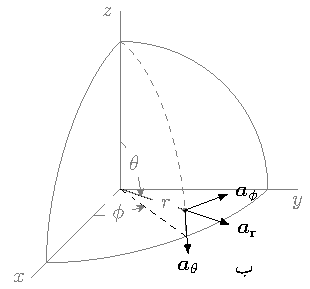
\includegraphics{figVectorSphericalUnitVectors}
\end{subfigure}%
\caption{(الف) تین عمودی سطحوں کے ملاپ سے نقطہ \عددیء{N} کا حصول۔ (ب) کروی محدد کے تین عمودی اکائی سمتیات۔}
\label{شکل_سمتیہ_کروی_تین_سطحوں_کا_مالپ}
\end{figure}

\عددیء{r} تبدیل کئے بغیر \عددیء{\theta} کو \عددیء{0^\circ} تا \عددیء{180^\circ} اور \عددیء{\phi} کو \عددیء{0^\circ} تا \عددیء{360^\circ} تبدیل کرنے سے  نقطہ \عددیء{N} کروی \عددیء{r=r_0} سطح  پر حرکت کرے گا۔ اس کروی سطح کا رداس \عددیء{r} ہو گا۔شکل \حوالہ{شکل_سمتیہ_کروی_محدد_متغیرات}-الف  میں \عددیء{\theta} کو \عددیء{0^\circ} تا \عددیء{90^\circ} اور \عددیء{\phi} کو \عددیء{0^\circ} تا \عددیء{90^\circ} تبدیل کرنے سے حاصل سطح  دکھائی گئی ہے۔شکل \حوالہ{شکل_سمتیہ_کروی_محدد_متغیرات}-ب میں \عددیء{\theta} تبدیل کئے بغیر \عددیء{r} اور \عددیء{\phi} تبدیل کرنے سے پیدا مخروط\فرہنگ{مخروط}\حاشیہب{cone}\فرہنگ{cone}  \عددیء{\theta=\theta_0}  کروی سطح دکھائی گئی ہے۔\عددیء{\phi} تبدیل کئے بغیر \عددیء{r} اور \عددیء{\theta} تبدیل کرنے سے  نلکی محدد کی طرح \عددیء{\phi=\phi_0} سطح حاصل ہوتی ہے۔ شکل \حوالہ{شکل_سمتیہ_کروی_تین_سطحوں_کا_مالپ}-الف میں ان تینوں سطحوں کو دکھایا گیا ہے۔بالکل کارتیسی اور نلکی محدد کی طرح، کسی بھی نقطہ \عددیء{N(r_0,\theta_0,\phi_0)} کا مقام ان تین سطحوں کے نقطہ ملاپ سے اخذ کیا جاتا ہے۔کسی بھی نقطہ \عددیء{N(r_0,\theta_0,\phi_0)} پر \عددیء{r=r_0}، \عددیء{\theta=\theta_0} اور \عددیء{\phi=\phi_0} سطحیں آپس میں عمودی ہوتی ہے اور یہ صرف اور صرف اسی نقطے پر اکھٹے ملتی ہیں۔

شکل \حوالہ{شکل_سمتیہ_کروی_تین_سطحوں_کا_مالپ}-ب میں کروی نظام کے تین عمودی اکائی سمتیات \عددیء{\ar}، \عددیء{\atheta} اور \عددیء{\aphi} دکھائے گئے ہیں۔نلکی محدد کی طرح کروی محدد کے عمودی اکائی سمتیات بھی مقام تبدیل کرنے سے تبدیل ہوتے ہیں۔کسی بھی نقطہ \عددیء{N(r_0,\theta_0,\phi_0)} پر \عددیء{\theta} اور \عددیء{\phi} تبدیل کئے بغیر \عددیء{r} کے بڑھتے جانب اکائی سمتیہ \عددیء{\ar} ہو گی۔اسی طرح \عددیء{\theta} بڑھانے سے نقطہ \عددیء{N} اکائی سمتیہ \عددیء{\atheta} کی جانب حرکت کرے گا جبکہ \عددیء{\phi} بڑھانے سے نقطہ \عددیء{\aphi} کی جانب حرکت کرے گا۔کارتیسی اور نلکی محدد کی طرح کروی محدد کے اکائی سمتیات کو بھی محددی نظام کے متغیرات کو کم سے کم بڑھاتے ہوئے  نقطے کی حرکت کی جانب اکائی سمتیہ کھینچنے سے حاصل کیا جاتا ہے۔

شکل \حوالہ{شکل_سمتیہ_کروی_تین_سطحوں_کا_مالپ}-الف سے واضح ہے کہ \عددیء{\ar} سمتیہ \عددیء{r=r_0} سطح کے عمودی جبکہ \عددیء{\theta=\theta_0} اور \عددیء{\phi=\phi_0} سطحوں کے متوازی ہے۔اسی طرح \عددیء{\atheta} سمتیہ \عددیء{\theta=\theta_0} سطح کے عمودی اور \عددیء{\phi=\phi_0} سطح کے متوازی پایا جاتا ہے جبکہ \عددیء{r=r_0} سطح کے ساتھ مماس بناتا ہے۔\عددیء{\aphi} سمتیہ \عددیء{\phi=\phi_0} سطح کے عمودی جبکہ \عددیء{r=r_0} اور \عددیء{\theta=\theta_0} سطحوں کے ساتھ مماس بناتا ہے۔

 
\عددیء{\ar}، \عددیء{\atheta} اور \عددیء{\aphi} کروی نظام  کے اکائی سمتیات ہیں۔\عددیء{\ar \times \atheta=\aphi} لکھنے سے  دائیں ہاتھ کا کروی نظام حاصل ہوتا ہے۔دائیں ہاتھ کے قانون میں دائیں ہاتھ کا انگوٹھا  \عددیء{r} جبکہ پہلی انگلی \عددیء{\theta}  اور دوسری انگلی \عددیء{\phi} بڑھانے سے پیدا حرکت کی سمتوں کو ظاہر کرتے ہیں۔نلکی محدد میں یہ انگلیاں \عددیء{\rho}، \عددیء{\phi} اور \عددیء{z} جبکہ کارتیسی محدد میں \عددیء{x}، \عددیء{y} اور \عددیء{z} بڑھانے سے پیدا حرکت کی سمتوں کو ظاہر کرتی ہیں۔

دائیں ہاتھ کے قانون  یا شکل \حوالہ{شکل_سمتیہ_کروی_صلیبی_ضرب_اکائی_سمتیات} کی مدد سے یوں اکائی سمتیات کے صلیبی ضرب
\begin{figure}
\centering
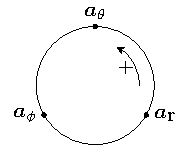
\includegraphics{figVectorSphericalRightHandCircle}
\caption{کروی نظام میں اکائی سمتیات کی صلیبی ضرب۔}
\label{شکل_سمتیہ_کروی_صلیبی_ضرب_اکائی_سمتیات}
\end{figure}

\begin{align}
\ar \times \atheta=\aphi, \quad \atheta \times \aphi=\ar, \quad \aphi \times \ar =\atheta
\end{align}

لکھے جا سکتے ہیں۔اسی طرح
\begin{align}
\ar \cdot \ar=1, \quad \atheta \cdot \atheta=1, \quad \aphi \cdot \aphi=1
\end{align}
اور
\begin{align}
\ar \cdot \atheta=0, \quad \atheta \cdot \aphi=0, \quad \aphi \cdot \ar=0
\end{align}
بھی لکھے جا سکتے ہیں۔

\begin{figure}
\centering
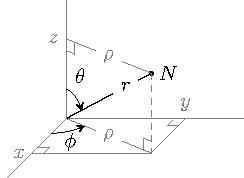
\includegraphics{figVectorSphericalToCylindricalAndCartesian}
\caption{کروی، نلکی اور کارتیسی متغیرات کا تبادلہ۔}
\label{شکل_سمتیہ_کروی_نلکی_متغیرات_تبادلہ}
\end{figure}

نقطہ \عددیء{N} کا \عددیء{z} محدد سے فاصلہ  \عددیء{\rho} ہے جو نلکی محدد کا رداس ہے۔اسے شکل \حوالہ{شکل_سمتیہ_کروی_نلکی_متغیرات_تبادلہ} میں دکھایا گیا ہے جہاں سے واضح ہے کہ \عددیء{\rho=r \sin \theta} کے برابر ہے۔اسی طرح \عددیء{z=0} سطح سے \عددیء{N} کی اونچائی \عددیء{z} ہے جو شکل کو دیکھتے ہوئے \عددیء{z=r\cos \theta}  لکھی جا سکتی ہے۔نقطہ \عددیء{N} کا عمودی سایہ \عددیء{z=0} سطح پر دکھایا گیا ہے جہاں سے واضح ہے کہ \عددیء{x=\rho \cos \phi} اور \عددیء{y=\rho \sin \phi} لکھے جا سکتے ہیں۔\عددیء{\rho=r \sin \theta} پُر کرنے سے
\begin{gather}
\begin{aligned}\label{مساوات_سمتیہ_کروی_سے_کارتیسی}
x&=r \sin \theta \cos \phi\\
y&=r \sin \theta \sin \phi\\
z&=r \cos \theta
\end{aligned}
\end{gather}
لکھے جا سکتے ہیں جہاں \عددیء{z} کی مساوات بھی ساتھ ہی لکھی  گئی ہے۔مساوات \حوالہ{مساوات_سمتیہ_کروی_سے_کارتیسی} کروی سے کارتیسی متغیرات دیتا ہے۔ اسی شکل کو دیکھتے ہوئے مسئلہ فیثاغورث کی مدد سے 
\begin{gather}
\begin{aligned}
r^2&=\rho^2+z^2\\
\rho^2&=x^2+y^2
\end{aligned}
\end{gather}
لکھتے ہوئے
\begin{align}\label{مساوات_سمتیہ_کروی_رداس}
r^2=x^2+y^2+z^2
\end{align}
حاصل ہوتا ہے۔مساوات \حوالہ{مساوات_سمتیہ_کروی_سے_کارتیسی} میں \عددیء{z} کی مساوات سے
\begin{align}\label{مساوات_سمتیہ_کروی_تھیٹا}
\theta = \cos^{-1} \frac{z}{r}=\cos^{-1}\frac{z}{\sqrt{x^2+y^2+z^2}}
\end{align}
 لکھا جا سکتا ہے۔اسی طرح  مساوات \حوالہ{مساوات_سمتیہ_کروی_سے_کارتیسی} کے \عددیء{y} کو \عددیء{x} سے تقسیم کرتے ہوئے
\begin{align}\label{مساوات_سمتیہ_کروی_فائے}
\phi = \tan^{-1} \frac{y}{x}
\end{align}
حاصل ہوتا ہے۔مساوات \حوالہ{مساوات_سمتیہ_کروی_رداس}، مساوات \حوالہ{مساوات_سمتیہ_کروی_تھیٹا} اور مساوات \حوالہ{مساوات_سمتیہ_کروی_فائے} کارتیسی سے کروی متغیرات دیتے ہیں۔
\begin{figure}
\centering
\begin{subfigure}{0.5\textwidth}
\centering
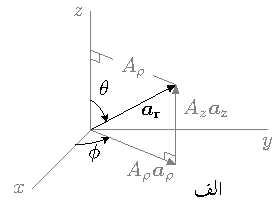
\includegraphics{figVectorSphericalUnitRadial}
\end{subfigure}%
%
\begin{subfigure}{0.5\textwidth}
\centering
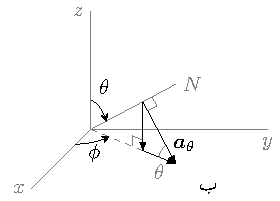
\includegraphics{figVectorSphericalUnitTheta}
\end{subfigure}%
\caption{کروی اکائی سمتیات کا کارتیسی نظام میں تبادلہ۔}
\label{شکل_سمتیہ_کروی_اکائی_رداسی_سمتیہ_کارتیسی}
\end{figure}

شکل \حوالہ{شکل_سمتیہ_کروی_تین_سطحوں_کا_مالپ}-ب میں نقطہ \عددیء{N} پر اکائی سمتیات دکھائے گئے ہیں۔\عددیء{\ar} کی سمت تبدیل کئے بغیر اسے محدد کے مرکز پر منتقل کرتے ہوئے شکل \حوالہ{شکل_سمتیہ_کروی_اکائی_رداسی_سمتیہ_کارتیسی}-الف  میں دکھایا گیا ہے جہاں سے ظاہر ہے کہ اسے نلکی محدد کے اکائی سمتیات کی مدد سے
\begin{align}
\ar=A_\rho \arho+A_z \az
\end{align}
لکھا جا سکتا ہے۔شکل \حوالہ{شکل_سمتیہ_کروی_اکائی_رداسی_سمتیہ_کارتیسی}-الف  میں \عددیء{\ar} کی لمبائی ایک لیتے ہوئے  \عددیء{A_\rho=\sin \theta} اور \عددیء{A_z=\cos \theta} لکھا جا سکتا ہے۔یوں
\begin{align}\label{مساوات_سمتیہ_کروی_اکائی_نلکی_منتقل}
\ar=\sin \theta \arho+\cos \theta \az
\end{align}
حاصل ہوتا ہے۔اس مساوات کا باری باری \عددیء{\arho}، \عددیء{\aphi} اور \عددیء{\az} کے ساتھ غیر سمتی ضرب لیتے ہوئے
\begin{gather}
\begin{aligned}\label{مساوات_سمتیہ_کروی_رداس_نلکی_اکائی_غیر_سمتی_ضرب}
\ar \cdot \arho&=(\sin \theta \arho+\cos \theta \az) \cdot \arho=\sin \theta\\
\ar \cdot \aphi&=(\sin \theta \arho+\cos \theta \az) \cdot \aphi=0\\
\ar \cdot \az&=(\sin \theta \arho+\cos \theta \az) \cdot \az=\cos \theta
\end{aligned}
\end{gather}
حاصل ہوتا ہے جہاں \عددیء{\arho \cdot \arho=1}، \عددیء{\az \cdot \arho=0} وغیرہ کا استعمال کیا گیا۔یہ مساوات کروی رداسی اکائی سمتیے اور نلکی نظام کے اکائی سمتیات کے تمام ممکنہ غیر سمتی ضرب دیتا ہے۔اسی طرح جدول \حوالہ{جدول_سمتیہ_نلکی_کارتیسی_اکائی_غیر-سمتی_ضرب} استعمال کرتے ہوئے  مساوات  \حوالہ{مساوات_سمتیہ_کروی_اکائی_نلکی_منتقل} کا باری باری \عددیء{\ax} اور \عددیء{\ay} کے ساتھ غیر سمتی ضرب لیتے ہوئے
\begin{gather}
\begin{aligned}\label{مساوات_سمتیہ_کروی_رداس_کے_کارتیسی_اجزاء}
\ar \cdot \ax&=(\sin \theta \arho+\cos \theta \az) \cdot \ax=\sin \theta \cos \phi\\
\ar \cdot \ay&=(\sin \theta \arho+\cos \theta \az) \cdot \ay=\sin \theta \sin \phi\\
\ar \cdot \az&=(\sin \theta \arho+\cos \theta \az) \cdot \az=\cos \theta
\end{aligned}
\end{gather}
حاصل ہوتا ہے۔مکمل نتائج ایک جگہ لکھنے کی خاطر  مندرجہ بالا مساوات میں  \عددیء{\ar \cdot \az} کو بھی شامل کیا گیا ہے۔ یہ مساوات کروی اکائی رداسی  سمتیے  اور کارتیسی اکائی سمتیات کے تمام ممکنہ غیر سمتی ضرب دیتا ہے۔

\عددیء{\ar} کو کارتیسی نظام میں لکھنے کی خاطر \عددیء{\ar=\kvec{A}=A_x \ax+A_y \ay+A_z \az} لکھتے ہیں۔مساوات \حوالہ{مساوات_سمتیہ_کارتیسی_اجزاء} کے مطابق \عددیء{A_x=\ax \cdot \ar} جبکہ \عددیء{A_y=\ay \cdot \ar} اور \عددیء{A_z=\az \cdot \ar} ہوں گے۔یہ تمام  مساوات \حوالہ{مساوات_سمتیہ_کروی_رداس_کے_کارتیسی_اجزاء} میں دئے گئے ہیں۔ یوں 
\begin{align}
\ar=\sin \theta \cos \phi \ax+\sin \theta \sin \phi \ay+\cos \theta \az
\end{align}
لکھا جا سکتا ہے۔

شکل \حوالہ{شکل_سمتیہ_کروی_تین_سطحوں_کا_مالپ}-ب میں دکھائے \عددیء{\atheta} کو \عددیء{\phi=\phi_0} سطح پر حرکت دیتے ہوئے  مرکز کے اتنے قریب لا کر شکل \حوالہ{شکل_سمتیہ_کروی_اکائی_رداسی_سمتیہ_کارتیسی}-ب میں دکھایا گیا ہے کہ اس کی نوک \عددیء{x=0} سطح کو چھوتی ہے۔جیسا شکل \حوالہ{شکل_سمتیہ_کروی_تین_سطحوں_کا_مالپ}-الف سے واضح ہے،  \عددیء{\phi=\phi_0} سطح پر \عددیء{\atheta} کو حرکت دینے سے اس سمتیہ کی سمت تبدیل نہیں ہوتی۔شکل \حوالہ{شکل_سمتیہ_کروی_اکائی_رداسی_سمتیہ_کارتیسی}-ب کو دیکھتے ہوئے \عددیء{\atheta=B_\rho \arho-B_z \az} لکھا جا سکتا ہے۔یہاں رک کر  تسلی کر لیں کہ \عددیء{B_\rho \arho} اور \عددیء{\atheta} کے مابین زاویہ \عددیء{\theta} ہے۔\عددیء{\atheta}، \عددیء{B_\rho \arho} اور \عددیء{-B_z \az} مل کر تکون بناتے ہیں جسے دیکھتے ہوئے مسئلہ فیثاغورث کی مدد سے
\begin{align*}
B_\rho&=\cos \theta\\
B_z&=\sin \theta
\end{align*}
لکھا جا سکتا ہے۔یوں
\begin{align}\label{مساوات_سمتیہ_کروی_اکائی_تھیٹا}
\atheta=\cos \theta \arho-\sin \theta \az
\end{align}
کے برابر ہے۔اس مساوات کا باری باری \عددیء{\arho}، \عددیء{\aphi} اور \عددیء{\az} کے ساتھ غیر سمتی ضرب لینے سے
\begin{gather}
\begin{aligned}\label{مساوات_سمتیہ_کروی_تھیٹا_نلکی_اکائی_غیر_سمتی_ضرب}
\atheta \cdot \arho&=(\cos \theta \arho-\sin \theta \az) \cdot \arho=\cos \theta\\
\atheta \cdot \aphi&=(\cos \theta \arho-\sin \theta \az) \cdot \aphi=0\\
\atheta \cdot \az&=(\cos \theta \arho-\sin \theta \az) \cdot \az=-\sin \theta
\end{aligned}
\end{gather}
\عددیء{\atheta} اور نلکی اکائی سمتیات کے  تمام غیر سمتی ضرب حاصل ہوتے ہیں۔اسی طرح مساوات \حوالہ{مساوات_سمتیہ_کروی_اکائی_تھیٹا} کا باری باری \عددیء{ax}، \عددیء{\ay} اور \عددیء{\az} کے ساتھ غیر سمتی ضرب لینے سے
\begin{gather}
\begin{aligned}\label{مساوات_سمتیہ_کروی_تھیٹا_کے_کارتیسی_اجزاء}
\atheta \cdot \ax&=(\cos \theta \arho-\sin \theta \az) \cdot \ax=\cos \theta \arho \cdot \ax=\cos \theta \cos \phi\\
\atheta \cdot \ay&=(\cos \theta \arho-\sin \theta \az) \cdot \ay=\cos \theta \arho \cdot \ay=\cos \theta \sin \phi \\
\atheta \cdot \az&=(\cos \theta \arho-\sin \theta \az) \cdot \az=-\sin \theta \az \cdot \az=-\sin \theta
\end{aligned}
\end{gather}
حاصل ہوتے ہیں۔یہ مساوات \عددیء{\atheta} اور کارتیسی اکائی سمتیات کے تمام غیر سمتی ضرب دیتا ہے۔

\عددیء{\atheta} کو کارتیسی نظام میں لکھنے کی خاطر \عددیء{\atheta=\kvec{A}=A_x \ax+A_y\ay+A_z\az} لکھتے ہیں۔مساوات \حوالہ{مساوات_سمتیہ_کارتیسی_اجزاء} کے مطابق \عددیء{A_x=\ax \cdot \atheta} جبکہ \عددیء{A_y=\ay \cdot \atheta} اور \عددیء{A_z=\az \cdot \atheta} ہوں گے۔یہ تمام  مساوات \حوالہ{مساوات_سمتیہ_کروی_تھیٹا_کے_کارتیسی_اجزاء} میں دئے گئے ہیں۔ یوں
\begin{align}
\atheta=\cos \theta \cos \phi \ax+\cos \theta \sin \phi\ay-\sin \theta\az
\end{align}  
لکھا جا سکتا ہے۔

کروی  محدد کا \عددیء{\aphi} اور نلکی محدد کا \عددیء{\aphi} یکساں ہیں۔اسے کارتیسی نظام میں
\begin{align}
\aphi=-\sin \phi \ax+\cos \phi \ay
\end{align} 
لکھا جاتا ہے۔اس مساوات کا \عددیء{\ax}، \عددیء{\ay} اور \عددیء{\az} کے ساتھ غیر سمتی ضرب لیتے ہوئے
\begin{gather}
\begin{aligned}
\aphi \cdot \ax&=-\sin \phi\\
\aphi \cdot \ay&=\cos \phi\\
\aphi \cdot \az&=0
\end{aligned}
\end{gather}
لکھا جا سکتا ہے۔

مساوات \حوالہ{مساوات_سمتیہ_کروی_رداس_نلکی_اکائی_غیر_سمتی_ضرب} اور مساوات \حوالہ{مساوات_سمتیہ_کروی_تھیٹا_نلکی_اکائی_غیر_سمتی_ضرب} کے نتائج کے ساتھ \عددیء{\aphi} کے مختلف غیر سمتی ضربوں کو جدول \حوالہ{جدول_سمتیہ_کروی_نلکی_اکائی_غیر-سمتی_ضرب} میں یکجا کیا گیا ہے۔

\begin{table}
\caption{کروی  اکائی سمتیات کا نلکی اکائی سمتیات کے ساتھ غیر سمتی ضرب۔}
\centering
\begin{tabular}{l | r r r}
 & $\arho$ & $\aphi$ & $\az$ \\
\hline
$\ar$ & $\sin \theta$ & $0$& $\cos \theta$\\
$\atheta$ &$\cos \theta$ &$ 0$ &$ -\sin \theta$\\
$\aphi$ & $0$ &$ 1$ &$0$
\end{tabular}
\label{جدول_سمتیہ_کروی_نلکی_اکائی_غیر-سمتی_ضرب}
\end{table}
%

مساوات  \حوالہ{مساوات_سمتیہ_کروی_رداس_کے_کارتیسی_اجزاء} اور مساوات  \حوالہ{مساوات_سمتیہ_کروی_تھیٹا_کے_کارتیسی_اجزاء} کے نتائج جدول \حوالہ{جدول_سمتیہ_کروی_کارتیسی_اکائی_غیر-سمتی_ضرب} میں یکجا کئے گئے ہیں۔ 
\begin{table}
\caption{کروی  اکائی سمتیات کا کارتیسی اکائی سمتیات کے ساتھ غیر سمتی ضرب۔}
\centering
\begin{tabular}{l | r r r}
 & $\ax$ & $\ay$ & $\az$ \\
\hline
$\ar$ & $\sin \theta \cos \phi$ & $\sin \theta \sin \phi$& $\cos \theta$\\
$\atheta$ &$\cos \theta \cos \phi$ &$ \cos \theta \sin \phi$ &$ -\sin \theta$\\
$\aphi$ & $-\sin \phi$ &$ \cos \phi$ &$0$
\end{tabular}
\label{جدول_سمتیہ_کروی_کارتیسی_اکائی_غیر-سمتی_ضرب}
\end{table}
%
\begin{figure}
\centering
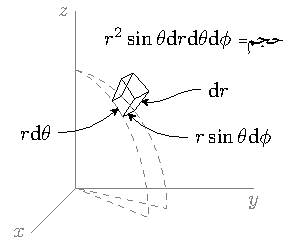
\includegraphics{figVectorSphericalDifferentialVolume}
\caption{کروی نظام میں چھوٹی حجم۔}
\label{شکل_سمتیہ_کروی_چھوٹی_حجم}
\end{figure}

شکل \حوالہ{شکل_سمتیہ_کروی_تین_سطحوں_کا_مالپ} میں \عددیء{N(r,\theta,\phi)} پر تین عمودی سطحیں دکھائی گئی ہیں۔اگر کروی محدد کے متغیرات \عددیء{\dif r}، \عددیء{\dif \theta} اور \عددیء{\dif \phi} بڑھا کر دوبارہ تین عمودی سطحیں کھینچی جائیں تو یہ چھ سطحیں مل کر چھوٹا منحرف مکعب نما حجم گھیریں گی جسے شکل \حوالہ{شکل_سمتیہ_کروی_چھوٹی_حجم} میں دکھایا گیا ہے۔\عددیء{\ar} سمت میں مکعب کے چار اطراف کی لمبائیاں \عددیء{\dif r} ہے۔\عددیء{\atheta} سمت میں \عددیء{z} محدد کے قریبی دو اطراف کی لمبائیاں \عددیء{r \dif \theta} جبکہ دو دور اطراف کی لمبائیاں \عددیء{(r+\dif r)\dif \theta} ہے جسے دو اجزاء کی صورت میں یوں  \عددیء{r \dif \theta +\dif r \dif \theta} لکھا جا سکتا ہے۔دور اطراف کے لمبائی کا پہلا جزو ہوبہو قریبی اطراف کی لمبائی ہے جبکہ اس کا دوسرا جزو دور اور قریبی اطراف کے لمبائیوں میں فرق کو ظاہر کرتی ہے۔ان دو اجزاء کی نسبت \عددیء{\tfrac{\dif r \dif \theta}{r \dif \theta}=\tfrac{\dif r}{r}}  کے برابر ہے۔\عددیء{\dif r} کو کم سے کم\حاشیہد{کسی بھی متغیرہ مثلاً \عددیء{r} میں چھوٹی سی تبدیلی کو \عددیء{\Delta r} لکھا جاتا ہے جبکہ اس میں کم سے کم تبدیلی کو \عددیء{\dif r} لکھا جاتا ہے۔\عددیء{\dif r} کو تقریباً صفر سمجھا جا سکتا ہے یعنی \عددیء{\dif r \to 0} ہوتا ہے۔} کرتے ہوئے اس نسبت کو کم سے کم کیا جا سکتا  ہے۔ایسا ہی کرتے ہوئے ہم \عددیء{\dif r \dif \theta} کو رد کرتے ہوئے ان چاروں اطراف کی لمبائیاں \عددیء{r \dif \theta} ہی لیتے ہیں۔اسی طریقہ کار سے  \عددیء{\aphi} اطراف کی لمبائیاں  \عددیء{r \sin \theta \dif \phi} لکھی جا سکتی ہے۔منحرف مکعب نما کے اطراف میں معمولی فرق کو نظرانداز کرتے ہوئے اسے مکعب نما تصور کیا جا سکتا ہے جس کے \عددیء{r=r_0} سطحوں کا رقبہ \عددیء{r^2 \sin \theta \dif \theta \dif \phi} جبکہ \عددیء{\theta=\theta_0} سطحوں کا رقبہ \عددیء{r \sin \theta \dif r \dif \phi} اور \عددیء{\phi=\phi_0} سطحوں کا رقبہ   \عددیء{r \dif r \dif \theta} ہو گا۔اس مکعب کا حجم \عددیء{r^2 \sin \theta \dif r \dif \theta \dif \phi} ہو گا۔

کسی بھی مکمل بند سطح کی  سمت، سطح کے عمودی باہر جانب لی جاتی ہے۔شکل \حوالہ{شکل_سمتیہ_کروی_چھوٹی_حجم} میں \عددیء{r=r_0} سطح  مرکز کا قریبی سطح ہے۔اس سطح کے دو آپس میں الٹ عمودی اطراف \عددیء{\mp \ar} ہیں جن میں \عددیء{-\ar} بند سطح کی بیرونی سمت کو ظاہر کرتا ہے لہٰذا یہی اس سطح کی درست سمت ہے۔اس کے برعکس \عددیء{r=r_0+\dif r} سطح مرکز سے دور تر ہے۔اس سطح کے بھی دو آپس میں الٹ عمودی سمتیں \عددیء{\mp \ar} ہیں جن میں \عددیء{\ar} سطح کی درست سمت ہے۔یوں  \عددیء{r=r_0} سطح کا سمتی رقبہ \عددیء{-r^2 \sin \theta \dif \theta \dif \phi \ar} جبکہ \عددیء{r=r_0+\dif r} سطح کا سمتی رقبہ \عددیء{\عددیء{r^2 \sin \theta \dif \theta \dif \phi \ar}} ہے۔اسی طرح \عددیء{\theta=\theta_0} سطح کا سمتی رقبہ \عددیء{-r \sin \theta \dif r \dif \phi\atheta} جبکہ \عددیء{\theta=\theta_0+\dif \theta} سطح کا سمتی رقبہ\عددی{r \sin \theta \dif r \dif \phi\atheta} ہو گا۔\عددیء{\phi=\phi_0} سطح کا \عددیء{-r \dif r \dif \theta \aphi} اور \عددیء{\phi=\phi_0+\dif \phi} سطح کا سمتی رقبہ \عددیء{r \dif r \dif \theta \aphi} ہو گا۔

%===================
\ابتدا{مشق}
شکل \حوالہ{شکل_سمتیہ_کروی_چھوٹی_حجم} میں \عددیء{} سمت میں مرکز کے قریبی اور دور اطراف کی لمبائیاں لکھیں۔

جوابات:\عددیء{r \sin \theta \dif \phi}، \عددیء{r \sin(\theta+\dif \theta) \dif \phi}، \عددیء{(r+\dif r) \sin \theta \dif \phi} اور \عددیء{(r+\dif r) \sin(\theta+\dif \theta) \dif \phi}
\انتہا{مشق}
%=======================
\ابتدا{مثال}\شناخت{مثال_سمتیہ_نلکی_کارتیسی_غیر_سمتی_اکائی_ضرب}
دو اکائی سمتیات \عددیء{\kvec{a}_1} اور \عددیء{\kvec{a}_2} کا غیر سمتی ضرب \عددیء{\kvec{a}_1 \cdot \kvec{a}_2=(1)(1) \cos \alpha_{12}} یعنی ان کے مابین زاویے \عددیء{\alpha_{12}} کے کوسائن کے برابر ہوتا ہے۔غیر سمتی ضرب کے اس تعریف کو استعمال کرتے ہوئے \عددیء{\ax \cdot \arho}، \عددیء{\ay \cdot \arho}، \عددیء{\ax \cdot \aphi} اور \عددیء{\ay \cdot \aphi} حاصل کریں۔
\begin{figure}
\centering
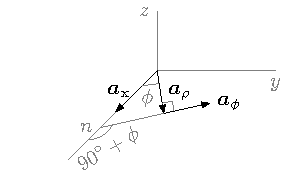
\includegraphics{figVectorDotProductUnitCartesianAndCylindrical}
\caption{کارتیسی اور نلکی اکائی سمتیات کا غیر سمتی ضرب۔}
\label{شکل_سمتیہ_غیر_سمتی_ضرب_بذریعہ_تعریف}
\end{figure}

حل:شکل \حوالہ{شکل_سمتیہ_غیر_سمتی_ضرب_بذریعہ_تعریف} میں \عددیء{\ax} اور \عددیء{\arho} کے درمیان زاویہ \عددیء{\phi} جبکہ \عددیء{\ay} اور \عددیء{\arho} کے درمیان زاویہ \عددیء{90^\circ-\phi} پایا جاتا ہے لہٰذا \عددیء{\ax \cdot \arho=\cos \phi} اور \عددیء{\ay \cdot \arho=\cos (90^\circ-\phi)=\sin \phi} کے برابر ہیں۔\عددیء{\ax} اور \عددیء{\aphi} کی سمتیں تبدیل کئے بغیر اگر انہیں یوں ہلایا جائے کہ ان کی دُم نقطہ \عددیء{n} پر آ ٹھرے تو شکل سے ظاہر ہے کہ ان کے مابین زاویہ \عددیء{90^\circ+\phi} ہے۔یوں \عددیء{\ax \cdot \aphi=\cos (90^\circ+\phi)=-\sin \phi} کے برابر ہے۔اسی طرح \عددیء{\ay} اور \عددیء{\aphi} کے درمیان \عددیء{\phi} زاویہ ہونے کی بنا پر \عددیء{\ay \cdot \aphi=\cos \phi} کے برابر ہے۔چونکہ \عددیء{\az} ان دونوں نلکی اکائی سمتیات کے عمودی ہے لہٰذا ان کا غیر سمتی ضرب صفر کے برابر ہو گا۔  
\انتہا{مثال}
%============
\begin{figure}
\centering
\begin{subfigure}{0.5\textwidth}
\centering
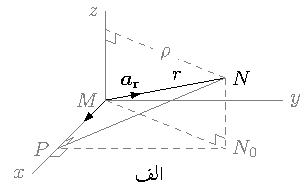
\includegraphics{figVectorSphericalUnitRadialDotWithCartesian}
\end{subfigure}%
%
\begin{subfigure}{0.5\textwidth}
\centering
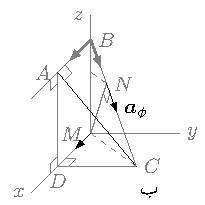
\includegraphics{figVectorSphericalUnitThetaDotWithCartesian}
\end{subfigure}%
\caption{کروی اور کارتیسی اکائی سمتیات کا غیر سمتی ضرب۔}
\label{شکل_سمتیہ_کروی_کارتیسی_اکائی_غیر_سمتی_ضرب}
\end{figure}

\ابتدا{مثال}
مثال \حوالہ{مثال_سمتیہ_نلکی_کارتیسی_غیر_سمتی_اکائی_ضرب} کے طرز پر \عددیء{\ar}  کا \عددیء{\ax}، \عددیء{\ay} اور \عددیء{\az} کے ساتھ غیر سمتی ضرب حاصل کریں۔

حل: شکل \حوالہ{شکل_سمتیہ_کروی_کارتیسی_اکائی_غیر_سمتی_ضرب}-الف میں نقطہ \عددیء{N(r,\theta,\phi)} دکھایا گیا ہے جسے \عددیء{N(x,y,z)} بھی لکھا جا سکتا ہے۔شکل میں \عددیء{\ax} اور \عددیء{\ar} بھی دکھائے گئے ہیں۔شکل سے ظاہر ہے کہ \عددیء{\ax \cdot \ar=\cos \phase{NMP}} کے برابر ہے جہاں \عددیء{N} اور \عددیء{P} سے \عددیء{M} تک لکیریں کھینچنے سے زاویہ \عددیء{\phase{NMP}} بنتا ہے۔\عددیء{N} سے \عددیء{z=0} سطح پر عمود نقطہ \عددیء{N_0} دیتا ہے۔\عددیء{N_0} سے \عددیء{x} محدد پر عمود نقطہ \عددیء{P} دیتا ہے۔\عددیء{N} سے \عددیء{N_0} اور یہاں سے \عددیء{P} منتقل ہوتے ہوئے \عددیء{\ax} سمت میں کسی قسم کی حرکت نہیں کی جاتی لہٰذا اگر کارتیسی نظام میں \عددیء{N(x,y,z)} لکھا جائے تو اسی نظام میں \عددیء{N_0(x,y,0)} اور  \عددیء{P(x,0,0)} لکھے جائیں گے۔ہم \عددیء{N} سے \عددیء{x} محدد پر عمود بناتے ہوئے بھی \عددیء{P} تک پہنچ سکتے ہیں۔ تکون \عددیء{NMP} میں \عددیء{M} سے \عددیء{N} تک کا فاصلہ \عددیء{\overline{MN}=r} جبکہ \عددیء{M} سے \عددیء{P} تک کا فاصلہ \عددیء{\overline{MP}=x} اور زاویہ \عددیء{\phase{NPM}=90^\circ} ہیں لہٰذا \عددیء{\cos \phase{NMP}=\tfrac{x}{r}} ہو گا۔یہی  \عددیء{\ax} اور \عددیء{\ar} کے غیر سمتی ضرب  کے برابر ہے۔\عددیء{N} سے \عددیء{y} محدد پر عمود بناتے ہوئے یوں \عددیء{\ay \cdot \ar=\tfrac{y}{r}} اور \عددیء{N} سے \عددیء{z} محدد پر عمود سے \عددیء{\az \cdot \ar=\tfrac{z}{r}} لکھے جا سکتے ہیں۔چونکہ \عددیء{x=r\sin \theta \cos \phi}، \عددیء{y=r\sin \theta \sin \phi} اور \عددیء{z=r\cos \theta} کے برابر  ہیں لہٰذا ہم
\begin{align*}
\ar \cdot \ax&=\frac{x}{r}=\sin \theta \cos \phi\\
\ar \cdot \ay&=\frac{y}{r}=\sin \theta \sin \phi\\
\ar \cdot \az&=\frac{z}{r}=\cos \theta
\end{align*}
لکھ سکتے ہیں۔
\انتہا{مثال}
%=======================
\ابتدا{مثال}
مثال \حوالہ{مثال_سمتیہ_نلکی_کارتیسی_غیر_سمتی_اکائی_ضرب} کے طرز پر \عددیء{\atheta}  کا \عددیء{\ax} کے ساتھ غیر سمتی ضرب حاصل کریں۔

حل: شکل \حوالہ{شکل_سمتیہ_کروی_کارتیسی_اکائی_غیر_سمتی_ضرب}-ب میں نقطہ \عددیء{N} پر اکائی سمتیہ \عددیء{\atheta} جبکہ محدد کے مرکز \عددیء{M} پر \عددیء{\ax} دکھائے گئے ہیں۔\عددیء{\atheta \cdot \ax} حاصل کرنے کی خاطر سمتیات کی سمت تبدیل کئے بغیر انہیں \عددیء{z} محدد پر نقطہ \عددیء{B} منتقل کرتے ہوئے دوبارہ دکھایا گیا ہے جہاں سے واضح ہے کہ \عددیء{\atheta \cdot \ax=\cos \phase{ABC}} کے برابر ہے۔اس شکل میں \عددیء{\phase{DMC}=\phi} اور \عددیء{\phase{BMN}=\theta} کروی محدد کے زاویے ہیں۔تکون \عددیء{\Delta BMN} میں زاویہ \عددیء{\phase{MNB}} نوے درجے کا ہے۔یوں \عددیء{\phase{NBM}=90^\circ-\theta} ہو گا۔شکل سے واضح ہے کہ  \عددیء{\phase{NBM}=\phase{CBM}} ہیں۔اس طرح تکون \عددیء{\Delta BMC} میں \عددیء{\phase{BMC}=90^\circ} جبکہ \عددیء{\phase{CBM}=90^\circ-\theta} ہونے کی بنا پر \عددیء{\phase{MCB}=\theta} ہو گا۔

شکل-ب میں \عددیء{\overline{BM}=z} لیتے ہوئے تکون \عددیء{\Delta BMC}   کو دیکھتے ہوئے
\begin{align*}
\overline{BC}&=\frac{z}{\sin \theta}   \\
\overline{MC}&=\frac{z}{\tan \theta} 
\end{align*}
لکھا جا سکتا ہے۔تکون \عددیء{\Delta MDC} سے
\begin{align*}
\overline{MD}&=\overline{MC} \cos \phi=\frac{z \cos \phi}{\tan \theta} 
\end{align*} 
لکھا جا سکتا ہے۔شکل سے واضح ہے کہ \عددیء{\overline{MD}} اور \عددیء{\overline{AB}} برابر ہیں یعنی \عددیء{\overline{AB}=\overline{MD}}-یوں تکون \عددیء{\Delta BAC} سے
\begin{align*}
\cos \phase{ABC}&=\frac{\overline{AB}}{\overline{BC}}=\frac{\left(\frac{z \cos \phi}{\tan \theta}\right)}{\left(\frac{z}{\sin \theta}\right)}=\cos \theta \cos \phi
\end{align*}
حاصل ہوتا ہے۔یوں \عددیء{\ar \cdot \ax=\cos \theta \cos \phi} لکھا جا سکتا ہے۔
\انتہا{مثال}
%============

\ابتدا{مشق}
شکل \حوالہ{شکل_سمتیہ_کروی_کارتیسی_اکائی_غیر_سمتی_ضرب}-ب کے طرز پر شکل بناتے ہوئے \عددیء{\atheta \cdot \ay} اور \عددیء{\atheta \cdot \ay} حاصل کریں۔

جوابات:\عددیء{\cos \theta \sin \phi} اور \عددیء{-\sin \theta}
\انتہا{مشق}
%============

% ToDo: Uncomment next 4 lines
%\باب{کولومب کا قانون}
\حصہ{قوت کشش یا دفع}
نیوٹن کے \اصطلاح{کائناتی تجاذب کے قانون}\فرہنگ{تجاذب}\حاشیہب{Law of Universal Gravitation} سے آپ بخوبی واقف ہوں گے۔\اصطلاح{کولومب کا قانون}\فرہنگ{کولومب کا قانون}\حاشیہب{Coulomb's law} اس سے قریبی مشابہت رکھتا ہے۔کائناتی تجاذب کے قانون کو مساوات \حوالہ{مساوات_کولوم_کشش_ثقل} میں پیش کیا گیا ہے۔
\begin{align}\label{مساوات_کولوم_کشش_ثقل}
F&=G \frac{M_1 M_2}{R^2}
\end{align}
یہ مساوات کمیت \عددیء{M_1} اور کمیت \عددیء{M_2} کے مابین قوت کشش \عددیء{F} دیتا ہے جہاں ایک کمیت کے مرکز سے دوسری کمیت کے مرکز تک کا فاصلہ \عددیء{R} ہے۔قوت کشش دونوں کمیت کے حاصل ضرب کے  راست متناسب اور ان کے مرکزوں کے درمیانی فاصلے  کے مربع کے بالعکس متناسب ہوتی ہے۔دونوں کمیتوں پر قوت کشش کی مقدار برابر ہوتی ہے اور یہ قوت دونوں کمیتوں کے  مرکزوں پر کھینچی لکیر پر عمل درآمد ہوتی ہے۔\عددیء{M_1} پر قوت کشش کی سمت \عددیء{M_1} کے مرکز سے \عددیء{M_2} کے مرکز کی جانب کو ہوتا ہے جبکہ \عددیء{M_2} پر قوت کشش کی سمت \عددیء{M_2} کے مرکز سے \عددیء{M_1} کے مرکز کی جانب کو ہوتا ہے۔تناسب کے جزو مستقل کو \عددیء{G} لکھا اور \اصطلاح{تجاذبی مستقل}\فرہنگ{تجاذبی مستقل}\حاشیہب{gravitational constant}\فرہنگ{gravitational constant} پکارا جاتا ہے جس کی قیمت تقریباً \عددیء{\SI{6.674e-11}{\meter \cubed \per \kilo \gram \per \second \squared}} کے برابر ہے۔

کولومب کا قانون مساوات \حوالہ{مساوات_کولوم_کولومب_کشش_چارج} میں بیان کیا گیا ہے۔یہ مساوات چارج \عددیء{Q_1} اور چارج \عددیء{Q_2} کے مابین قوت کشش یا قوت دفع \عددیء{F} دیتا ہے جہاں ایک چارج کے مرکز سے دوسری چارج کے مرکز تک کا فاصلہ \عددیء{R} ہے۔ان چارجوں کا حجم صفر تصور کیا جاتا ہے۔یوں اگر چارج کو گیند کی شکل کا تصور کیا جائے تو اس گیند کے رداس  کی لمبائی صفر ہو گی۔ایسے چارج کو \اصطلاح{نقطہ چارج}\فرہنگ{نقطہ چارج}\حاشیہب{point charge}\فرہنگ{point charge} کہا جاتا ہے۔
\begin{align}\label{مساوات_کولوم_کولومب_کشش_چارج}
F&=\frac{1}{4 \pi \epsilon_0}\frac{Q_1 Q_2}{ R^2}
\end{align}

قوت کشش یا دفع دونوں چارجوں کے حاصل ضرب کے  راست متناسب  اور باہمی فاصلہ کے  مربع کے بالعکس متناسب ہوتی ہے۔دونوں چارجوں پر قوت کی مقدار برابر ہوتی ہے اور یہ قوت دونوں چارجوں سے گزرتی لکیر پر عمل درآمد ہوتی ہے۔دو مختلف اقسام کے چارجوں کے مابین قوت کشش پائی جاتی ہے جبکہ دو یکساں چارجوں کے مابین قوت دفع پائی جاتی ہے۔مساوات کے جزو مستقل کو \عددیء{\tfrac{1}{4 \pi \epsilon_0}} لکھا جاتا ہے جہاں \عددیء{\epsilon_0} خالی خلاء  کا \اصطلاح{برقی مستقل}\فرہنگ{برقی مستقل}\حاشیہب{permittivity}\فرہنگ{permittivity}\حاشیہب{electric constant}\فرہنگ{electric constant} ہے جس کی قیمت اٹل ہے۔خالی خلاء کے برقی مستقل کی قیمت
\begin{align}
\epsilon_0=\frac{1}{\mu_0 c^2}
\end{align}
ہے جہاں \عددیء{c} خالی خلاء میں روشنی کی رفتار اور \عددیء{\mu_0} خالی خلاء کی \اصطلاح{مقناطیسی مستقل}\فرہنگ{مقناطیسی مستقل}\حاشیہب{permeability}\فرہنگ{permeability} ہے۔یہ دونوں بھی اٹل مستقل ہیں جن کی قیمتیں
\begin{align}
c&=\SI{299792458}{\meter \per \second}\\
\mu_0&=\SI{4 \numpi e-7}{\henry \per \meter}
\end{align}
 ہیں۔یوں مقناطیسی مستقل  کی قیمت تقریباً
\begin{align}
\epsilon_0 =\num{8.854e-12} \overset{.}{=}\frac{1}{36 \pi} 10^{-9} \si{\farad \per \meter}
\end{align}
 کے برابر ہے۔اس کتاب میں \عددیء{\tfrac{1}{4 \pi \epsilon_0}} بار بار استعمال ہو گا جسے عموماً
\begin{align}
\frac{1}{4 \pi \epsilon_0} \overset{.}{=} 9 \times 10^9
\end{align}
لیا جائے گا۔\عددیء{\epsilon_0}  کی اکائی فیراڈ فی میٹر  \عددیء{\si{\farad \per \meter}} ہے  جس کی وضاحت جلد کر دی جائے گی۔

\ابتدا{مثال}
زمین کی سطح پر زمین اور ایک کلو گرام کمیت کے مابین \عددیء{\SI{9.8}{\newton}} کی قوت کشش پائی جاتی ہے۔زمین کا رداس \عددیء{\SI{6370}{\kilo \meter}} لیتے ہوئے زمین کی کمیت حاصل کریں۔

حل:مساوات \حوالہ{مساوات_کولوم_کشش_ثقل} کی مدد سے
\begin{align*}
9.8=\frac{6.674 \times 10^{-11} \times M \times 1}{\num{6370000} \times \num{6370000}}\\
\end{align*}
لکھتے ہوئے زمین کی کمیت \عددیء{\SI{5.959e24}{\kilo \gram}} حاصل ہوتی ہے۔
\انتہا{مثال}
%===========================
\ابتدا{مثال}
زمین کی مرکز سے تقریباً \عددیء{\SI{42000}{\kilo \meter}} کے فاصلے پر  ذرائع ابلاغ کے سیٹلّائٹ زمین کے گرد مدار میں گردش کرتے ہیں۔اس فاصلے پر ایک کلا گرام کی کمیت اور زمین کے مابین قوت کشش کی مقدار حاصل کریں۔

حل: 
\begin{align*}
F=\frac{6.674 \times 10^{-11} \times 5.959 \times 10^{24} \times 1}{\num{42000000} \times \num{42000000}}=\SI{0.225}{\newton}\\
\end{align*}
\انتہا{مثال}
%============================
\ابتدا{مثال}
ایک ایک کولومب کے دو مثبت چارجوں کے درمیان  ایک میٹر کا فاصلہ ہے۔ان میں قوت دفع حاصل کریں۔

حل: 
\begin{align*}
F&=9 \times 10^9 \frac{1 \times 1}{1 \times 1}=\SI{9e9}{\newton}
\end{align*}
\انتہا{مثال}
%===================

مندرجہ بالا مثال سے  آپ دیکھ سکتے ہیں کہ چارج کی اکائی (کولومب)  انتہائی بڑی مقدار ہے۔

شکل \حوالہ{شکل_سمتیہ_دو_مثبت_چارج_قوت_دفع} میں چارج \عددیء{Q_1} محدد کے مرکز سے سمتی فاصلہ \سمتیہ{r_1} پر جبکہ چارج \عددیء{Q_2} مرکز سے سمتی فاصلہ \سمتیہ{r_2} پر دکھائے گئے ہیں۔چارج \عددیء{Q_1} سے چارج \عددیء{Q_2} تک کا سمتی فاصلہ \سمتیہ{R_{21}} ہے جہاں
\begin{align}
\kvec{R_{21}}=\kvec{r_2}-\kvec{r_1}
\end{align}
کے برابر ہے۔سمتیہ \سمتیہ{R_{21}} کی سمت میں اکائی سمتیہ \سمتیہ{a_{21}} یوں حاصل کیا جاتا ہے
\begin{align}
\kvec{a_{21}}=\frac{\kvec{R_{21}}}{\abs{\kvec{R_{21}}}}=\frac{\kvec{R_{21}}}{R_{21}}=\frac{\kvec{r_2}-\kvec{r_1}}{\abs{\kvec{r_2}-\kvec{r_1}}}
\end{align}
چارج \عددیء{Q_2} پر قوت \سمتیہ{F_2} کی حتمی قیمت مساوات  \حوالہ{مساوات_کولوم_کولومب_کشش_چارج} سے حاصل کی جا سکتی ہے جبکہ اس کی سمت اکائی سمتیہ \سمتیہ{a_{21}} کے سمت میں ہو گی۔اس طرح یہ قوت
\begin{gather}
\begin{aligned}\label{مساوات_کولومب_قوت_کی_مساوات_الف}
\kvec{F_2}&=\frac{1}{4 \pi \epsilon_0}\frac{Q_1 Q_2}{ R_{21}^2} {\kvec{a_{21}}}\\
&=\frac{Q_1 Q_2}{4 \pi \epsilon_0}\frac{\kvec{r_2}-\kvec{r_1}}{\abs{\kvec{r_2}-\kvec{r_1}}^3}
\end{aligned}
\end{gather}
لکھا جائے گا۔مساوات \حوالہ{مساوات_کولومب_قوت_کی_مساوات_الف} کولومب کے قانون کی سمتی شکل ہے۔چونکہ دونوں چارجوں پر برابر مگر الٹ سمت میں قوت عمل کرتا ہے لہٰذا \عددیء{Q_1} پر قوت \سمتیہ{F_1} یوں لکھا جائے گا
 \begin{gather}
\begin{aligned}
\kvec{F_1}=-\kvec{F_2}&=\frac{-1}{4 \pi \epsilon_0}\frac{Q_1 Q_2}{ R_{21}^2} \kvec{a_{21}}\\
&=\frac{1}{4 \pi \epsilon_0}\frac{Q_1 Q_2}{ R^2} {\kvec{a_{12}}}
\end{aligned}
\end{gather}
جہاں دوسری قدم پر \عددیء{R_{21}=R_{12}=R} لکھا گیا ہے اور \عددیء{\kvec{a_{12}}=-\kvec{a_{21}}} کے برابر ہے۔
%
\begin{figure}
\centering
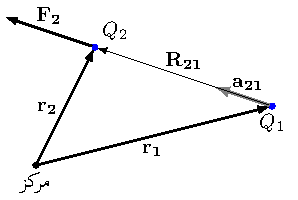
\includegraphics{figCoulombForceBetweenTwoCharges}
\caption{دو مثبت چارجوں کے مابین قوت دفع}
\label{شکل_سمتیہ_دو_مثبت_چارج_قوت_دفع}
\end{figure}
دونوں چارج مثبت یا دونوں چارج منفی ہونے کی صورت میں \عددیء{Q_2} پر مساوات \حوالہ{مساوات_کولومب_قوت_کی_مساوات_الف} سے قوت \سمتیہ{a_{21}} کی سمت میں حاصل ہوتا ہے۔یوں یکساں چارجوں کے مابین قوت دفع پایا جاتا ہے۔دو الٹ اقسام کے چارجوں کی صورت میں \عددیء{Q_2} پر قوت \سمتیہ{-a_{21}} کی سمت میں حاصل ہوتا ہے۔یوں الٹ اقسام کے چارجوں کے مابین قوت کشش پایا جاتا ہے۔  

\ابتدا{مثال}
شکل \حوالہ{شکل_سمتیہ_دو_مثبت_چارج_قوت_دفع} میں نقطہ \عددیء{A(3,2,4)} پر \عددیء{\SI{20}{\micro \coulomb}} کا چارج \عددیء{Q_1} جبکہ نقطہ \عددیء{B(1,5,9)} پر \عددیء{\SI{-50}{\coulomb}} کا چارج \عددیء{Q_2} پایا جاتا ہے۔منفی چارج \عددیء{Q_2} پر سمتی قوت حاصل کریں۔

حل:
\begin{align*}
\kvec{R_{21}}&=(1-3) \ax+(5-2) \ay+(9-4)\az\\
&=-2 \ax+3 \ay+5 \az\\
R_{21}&=\abs{\kvec{R_{21}}}=\sqrt{2^2+3^2+5^2}\\
&=\sqrt{38}\\
&=6.1644
\end{align*}
اور یوں
\begin{align*}
\kvec{a_{21}}&=\frac{{\kvec{R_{21}}}}{R_{21}}=\frac{-2 {\ax}+3 {\ay}+5 \az}{6.1644}\\
&=-0.324 \ax+0.487 \ay+0.811\az
\end{align*}
حاصل ہوتا ہے جس سے
\begin{align*}
\kvec{F_2}&=\frac{36 \pi  \times 10^9}{4 \pi} \frac{\left (-50\times 10^{-6} \times 20 \times 10^{-6} \right )}{38} \left(-0.324 \ax+0.487 \ay+0.811\az\right)\\
&=-0.237  \left(-0.324 \ax+0.487 \ay+0.811\az \right) \, \si{\newton}
\end{align*}
حاصل ہوتا ہے۔آپ دیکھ سکتے ہیں کہ قوت کی سمت \سمتیہ{a_{21}} کے الٹ سمت میں ہے۔یوں منفی چارج پر قوت کی سمت مثبت چارج کی جانب ہے یعنی اس پر قوت کشش پایا جاتا ہے۔
\انتہا{مثال}
%========================
کسی بھی چارج پر ایک سے زیادہ چارجوں سے پیدا مجموعی قوت تمام چارجوں سے پیدا علیحدہ علیحدہ قوتوں کا سمتی مجموعہ ہوتا ہے یعنی
\begin{align}
\kvec{F}=\sum_{i=1}^n \kvec{F}_i
\end{align}
اس حقیقت کو یوں بیان کیا جاتا ہے کہ کولومب کا قانون \اصطلاح{خطی}\فرہنگ{خطی}\حاشیہب{linear}\فرہنگ{linear} ہے۔ 

%========================
\حصہ{برقی میدان کی شدت}
نیوٹن کے کائناتی تجاذب کے قانون میں زمین کی کمیت کو \عددیء{M} لکھ کر کمیت \عددیء{m} پر قوت \عددیء{F} حاصل کی جا سکتی ہے۔ایک کلوگرام کمیت پر اس قوت کی مقدار \عددیء{\tfrac{F}{m}} ہو گی جسے \اصطلاح{زمین کی کشش}\فرہنگ{کشش!زمین}\حاشیہب{gravity}\فرہنگ{gravity} یا \اصطلاح{ثقلی اسراع} پکارا اور \عددیء{g} لکھا جاتا ہے۔زمین کی سطح پر \عددیء{g} کی مقدار تقریباً \عددیء{\SI{9.8}{\meter \per \second \squared}} کے برابر ہے۔
\begin{align}\label{مساوات_کولومب_زمین_کی_کشش}
g&=\frac{F}{m}=\frac{GM}{R^2}
\end{align}

کسی بھی کمیت \عددیء{M} کے گرد  \اصطلاح{تجاذبی میدان}\حاشیہب{gravitational field}\فرہنگ{تجاذبی میدان} پایا جاتا ہے۔ کسی بھی نقطے پر  اس تجاذبی میدن کو ناپنے کی خاطر اس نقطے پر پیمائشی کمیت \عددیء{m_p}\حاشیہد{\عددیء{m_p} لکھتے ہوئے  زیرنوشت میں \عددیء{p} لفظ پیمائشی  کے \موٹا{پ} کو ظاہر کرتا ہے، یعنی یہ وہ کمیت ہے جسے قوت  کی پیمائش کی خاطر استعمال کیا جا رہا ہے۔} رکھ کر اس پر قوت ناپی جاتی ہے۔مختلف مقامات پر اس طرح قوت ناپ کر ہم تجاذبی میدان کا جائزہ لے سکتے ہیں۔تجاذبی قوت کی مقدار کا دارومدار پیمائشی کمیت \حاشیہب{test mass} \عددیء{m_p} پر بھی منحصر ہے۔مختلف تجاذبی میدانوں کا آپس میں موازنہ کرتے وقت یہ ضروری ہے کہ تمام تجاذبی میدان جانچتے وقت ایک ہی قیمت کے پیمائشی کمیت استعمال کی جائے۔ماہرین طبیعیات عموماً \عددیء{m_p} کو ایک کلوگرام  رکھتے ہیں۔یہ ضروری نہیں کہ تجاذبی قوت ناپتے وقت ایک کلوگرام کی پیمائشی کمیت ہی استعمال کی جائے البتہ جوابات اکٹھے کرتے وقت \سمتیہ{F} کو \عددیء{m_p} سے تقسیم کرتے ہوئے ایک کلوگرام پر تجاذبی قوت حاصل کی جا سکتی ہے۔زمین کے قریب ایک کلو گرام کمیت پر قوت کشش کو ثقلی اسراع \عددی{g} پکارا جاتا ہے۔

\ابتدا{مثال}
زمین کی سطح پر دو سو گرام پیمائشی کمیت پر \عددیء{\SI{1.96}{\newton}} قوت ناپی جاتی ہے۔ثقلی اسراع حاصل کریں۔

حل:
\begin{align}
g=\frac{1.96}{0.2}=\SI{9.8}{\newton \per \kilogram}
\end{align}   
\انتہا{مثال}

مساوات \حوالہ{مساوات_کولومب_زمین_کی_کشش} سے ہم
\begin{gather}
\begin{aligned}
F&=m g\\
w&=m g
\end{aligned}
\end{gather}
لکھ سکتے ہیں جو زمین کی  سطح پر کمیت \عددیء{m} پر کشش ثقل \عددیء{F} دیتا ہے جسے  وزن پکارا اور  \عددیء{w} لکھا جاتا ہے۔
  
چارجوں پر بھی اسی طرح غور کیا جاتا ہے۔کسی بھی چارج \عددیء{Q} کے گرد برقی میدان پایا جاتا ہے۔اس برقی میدان میں چارج پر قوت اثر انداز ہوتا ہے۔چارج \عددیء{Q} کے برقی میدان کی شدت کے پیمائش کی خاطر اس میدان میں مختلف مقامات پر پیمائشی چارج \حاشیہب{test charge} \عددیء{q_p} پر قوت \سمتیہ{F} ناپ کر برقی میدان کا مطالعہ کیا جا سکتا ہے اور اس کا نقشہ بنایا جا سکتا ہے۔مختلف چارجوں کے برقی میدانوں کا آپس میں موازنہ کرتے وقت یہ ضروری ہے کہ تمام صورتوں میں ایک ہی قیمت کے پیمائشی چارج  استعمال کئے جائیں۔ماہرین طبیعیات \عددیء{q_p} کو ایک کولومب کا مثبت چارج  رکھتے ہیں۔یہ ضروری نہیں کہ قوت ناپتے وقت ایک کولومب کا مثبت پیمائشی چارج ہی استعمال کیا جائے البتہ جوابات اکٹھے کرتے وقت \سمتیہ{F} کو \عددیء{q_p} سے تقسیم کرتے ہوئے ایک مثبت کولومب پر قوت حاصل کی جاتی ہے جسے \اصطلاح{برقی میدان کی شدت}\فرہنگ{برقی میدان کی شدت}\حاشیہب{electric field intensity}\فرہنگ{electric field intensity} یا صرف \اصطلاح{برقی میدان} پکارا اور \سمتیہ{E} لکھا جاتا ہے یعنی
\begin{align}\label{مساوات_کولومب_برقی_شدت_اور_قوت}
\kvec{E}=\frac{\kvec{F}}{q_p}
\end{align}
مختلف مقامات پر موجود مختلف قیمتوں کے چارجوں سے کسی ایک نقطے پر  پیدا برقی میدان  تمام چارجوں کے مجموعی اثر سے پیدا ہو گا۔ایسا کولومب کے قانون کے خطی ہونے کی بنا پر ہوتا ہے۔کسی بھی نقطے پر \عددیء{n} چارجوں کا مجموعی \سمتیہ{E} تمام چارجوں کے علیحدہ علیحدہ پیدا کردہ  \سمتیازیرنوشت{E}{1}،  \سمتیازیرنوشت{E}{2}،\سمتیازیرنوشت{E}{3}،\عددیء{\cdots}  کا سمتی مجموعہ
\begin{align}
\kvec{E}=\sum_{i=1}^n \kvec{E}_i=\kvecsub{E}{1}+\kvecsub{E}{2}+\kvecsub{E}{3}+\cdots 
\end{align}
 ہوتا ہے۔یوں کسی بھی نقطے \عددیء{P}  پر \سمتیہ{E} ناپتے وقت اس نقطے پر ایک کولومب چارج \عددیء{q_p} رکھ کر اس چارج پر قوت ناپی جاتی ہے۔یہ قوت اس نقطے پر تمام چارجوں کا مجموعی  \سمتیہ{E} ہوتا ہے۔یاد رہے کہ کسی بھی نقطے پر  \سمتیہ{E} ناپتے وقت یہاں رکھے پیمائشی چارج \عددیء{q_p} کا اثر شامل نہیں ہوتا۔

مساوات  \حوالہ{مساوات_کولومب_قوت_کی_مساوات_الف} سے  چارج \عددیء{Q} سے \عددیء{\kvec{a}_R} سمت میں \عددیء{R} فاصلے پر برقی میدان کو
\begin{gather}
\begin{aligned}\label{مساوات_کولومب_قوت_کی_عمومی_مساوات}
\kvec{E}&=\frac{Q}{4 \pi \epsilon_0}\frac{\kvec{a_{R}}}{ R^2}\\
&=\frac{Q}{4 \pi \epsilon_0}\frac{\kvec{R}}{ R^3}
\end{aligned}
\end{gather}
لکھا جا سکتا ہے۔چارج کو کروی محدد کے مرکز پر تصور کرتے ہوئے اسی مساوات کو یوں لکھا جا سکتا ہے
\begin{align}\label{مساوات_کولومب_نقطہ_چارج_کروی_رداس_پر_تبدیل_نہیں_ہوتا}
\kvec{E}=\frac{Q}{4 \pi \epsilon_0 r^2} \ar
\end{align}
جہاں  \عددیء{\ar}  کروی محدد کا رداسی سمت میں اکائی سمتیہ ہے۔

نقطہ \عددیء{(x',y',z')} پر موجود چارج \عددیء{Q} سے نقطہ \عددیء{(x,y,z)} پر برقی شدت  یوں حاصل کی جا سکتی ہے۔
\begin{gather}
\begin{aligned} \label{مساوات_کولومب_نقطہ_چارج_سے_میدان_کا_حصول}
\kvec{E}&=\frac{1}{4 \pi \epsilon_0 }\frac{Q}{\abs{\kvec{r}-\kvec{r'}}^2} \frac{\kvec{r}-\kvec{r'}}{\abs{\kvec{r}-\kvec{r'}}}=\frac{Q}{4 \pi \epsilon_0 }\frac{\kvec{r}-\kvec{r'}}{\abs{\kvec{r}-\kvec{r'}}^3}\\
&=\frac{Q}{4 \pi \epsilon_0}\frac{\left[(x-x')\ax+(y-y')\ay+(z-z')\az\right]}{\left [(x-x')^2+(y-y')^2+(z-z')^2\right]^{\frac{3}{2}}}
\end{aligned}
\end{gather} 
جہاں
\begin{align*}
\kvec{r}&=x \ax+y \ay+z\az\\
\kvec{r'}&=x' \ax+y' \ay+z'\az\\
\kvec{R}&=\kvec{r}-\kvec{r'}=(x-x') \ax+(y-y') \ay+(z-z')\az
\end{align*}
کے برابر ہے۔
%===================
\ابتدا{مثال}\حاشیہط{چارج کم کرتے ہوئے جوابات 0 تا 1 کریں}
نقطہ \عددیء{N_1(4,1,1)} پر \عددیء{\SI{100}{\micro \coulomb}} کا چارج \عددیء{Q_1} جبکہ نقطہ \عددیء{N_2(1,4,2)} پر \عددیء{\SI{50}{\micro \coulomb}} کا چارج \عددیء{Q_2} پایا جاتا ہے۔نقطہ \عددیء{N_3(2,2,5)} پر  \عددیء{Q_1} سے پیدا \سمتیازیرنوشت{E}{1}  اور \عددیء{Q_2} سے پیدا \سمتیازیرنوشت{E}{2} حاصل کریں۔اس نقطے پر دونوں چارجوں کا مجموعی \عددیء{\kvec{E}} کیا ہو گا۔
\begin{figure}
\centering
\includegraphics[height=3.5cm]{figCoulombElectricFieldOfTwoCharges}
\caption{دو چارجوں سے پیدا برقی شدت}
\label{شکل_کولومب_دو_چارجوں_سے_پیدا_برقی_شدت}
\end{figure}

حل:شکل \حوالہ{شکل_کولومب_دو_چارجوں_سے_پیدا_برقی_شدت} میں صورت حال دکھایا گیا ہے۔پہلے \عددیء{Q_1} سے پیدا \سمتیازیرنوشت{E}{1} حاصل کرتے ہیں۔\عددیء{N_1}  سے \عددیء{N_3} تک سمتی فاصلہ
\begin{align*}
\kvecsub{R}{31}=\kvecsub{R}{3}-\kvecsub{R}{1}&=(2-4)\ax+(2-1)\ay+(5-1)\az\\
&=-2\ax+1\ay+4\az
\end{align*}
ہے جس سے
\begin{align*}
R_{31}&=\abs{\kvecsub{R}{31}}=\sqrt{2^2+1^2+4^2}\\
&=\sqrt{21}=4.583\\
\kvecsub{a}{31}&=\frac{\kvecsub{R}{31}}{R_{31}}=\frac{-2\ax+1\ay+4\az}{\sqrt{21}}\\
&=-0.436\ax+0.218\ay+0.873\az
\end{align*}
حاصل ہوتے ہیں۔یوں
\begin{align*}
\kvecsub{E}{1}&=9 \times 10^9 \frac{100 \times 10^{-6}}{21} \left(-0.436\ax+0.218\ay+0.873\az\right)\\
&=-\num{18686}\ax+\num{9343}\ay+\num{37414}\az \quad \si{\volt \per \meter}
\end{align*}
ہوتا ہے۔اسی طرح \عددیء{Q_2} کے لئے حل کرتے ہوئے
\begin{align*}
\kvecsub{R}{32}&=(2-1)\ax+(2-4)\ay+(5-2)\az\\
&=1\ax-2\ay+3\az
\end{align*}
اور
\begin{align*}
R_{32}&=\abs{\kvecsub{R}{32}}=\sqrt{1^2+2^2+3^2}=\sqrt{14}\\
\kvecsub{a}{32}&=\frac{1\ax-2\ay+3\az}{\sqrt{14}}\\
&=0.267\ax-0.535\ay+0.802\az
\end{align*}
سے
\begin{align*}
\kvecsub{E}{2}&=9 \times 10^9 \frac{50 \times 10^{-6}}{14} \left(0.267\ax-0.535\ay+0.802\az \right)\\
&=\num{8582}\ax-\num{17196}\ay+\num{25779}\az \quad \si{\volt \per \meter}
\end{align*}
ملتا ہے۔ان دو جوابات کا سمتی مجموعہ لیتے ہوئے کُل \kvec{E} حاصل کرتے ہیں۔
\begin{align*}
\kvec{E}&=\kvecsub{E}{1}+\kvecsub{E}{2}\\
&=\left(\num{-18686} \ax+\num{9343} \ay+\num{37414}\az\right)+\left(\num{8582}\ax-\num{17196}\ay+\num{25779}\az\right)\\
&=-\num{10104}\ax-\num{7853}\ay+\num{63193}\az \quad \si{\volt \per \meter}
\end{align*} 
\انتہا{مثال}
%===================
 
مساوات \حوالہ{مساوات_کولومب_برقی_شدت_اور_قوت} کو
\begin{align}
\kvec{F}=q \kvec{E}
\end{align}
لکھا جا سکتا ہے جو برقی میدان \سمتیہ{E} کے موجودگی میں چارج \عددیء{q} پر قوت \سمتیہ{F} دیتا ہے۔


\حصہ{یکساں چارج بردار سیدھی لامحدود لکیر  کا برقی میدان}
شکل \حوالہ{شکل_کولومب_لامحدود_لکیر_پر_چارج_کا_میدان} میں \عددیء{z} محدد پر \عددیء{z=-\infty} سے \عددیء{z=+\infty} تک یکساں چارج کی کثافت پائی جاتی ہے۔آپ تصور کر سکتے ہیں کہ \عددیء{z} محدد پر انتہائی قریب قریب برابر فاصلے پر یکساں \اصطلاح{نقطہ چارج} رکھے گئے ہیں۔یوں اگر \عددیء{\Delta L} لمبائی میں کُل \عددیء{\Delta Q} چارج پایا جائے تب اکائی لمبائی میں \عددیء{\tfrac{\Delta Q}{\Delta L}} چارج پایا جائے گا جسے \اصطلاح{لکیری چارج کثافت}\فرہنگ{کثافت!لکیری چارج}\حاشیہب{line charge density}\فرہنگ{density!line charge}  \عددیء{\rho_L}\حاشیہد{اس کتاب میں رداس کے لئے بھی \عددیء{\rho} استعمال کیا جاتا ہے۔\عددیء{\rho} کو جب بھی کثافت کے لئے استعمال کیا جائے،اس کے زیر نوشت میں \تحریر{L}، \تحریر{S} یا \تحریر{h} لکھا جائے گا۔} کہا جاتا ہے اور جس کی اکائی \عددیء{\si{\coulomb / \meter}} ہے۔لکیری چارج کثافت کی تعریف
\begin{align}
\rho_L=\lim_{\Delta L \to 0}\frac{\Delta Q}{\Delta L}
\end{align}
ہے۔لکیر پر چھوٹی لمبائی  اتنی کم نہیں کی جاتی کہ چارج بردار الیکٹران علیحدہ علیحدہ نظر آئیں اور لکیری کثافت کی جگہ نقطہ چارج نظر آئیں۔اگر لکیر پر چارج کی تقسیم ہر جگہ یکساں نہ ہو تب لکیری چارج کثافت متغیر ہو گی۔آئیں یکساں لکیری چارج کثافت سے خالی خلاء میں پیدا برقی میدان پر غور کریں۔ 
 \begin{figure}
\centering
\includegraphics[height=3.5cm]{figCoulombElectricFieldOfInfiniteLineCharge}
\caption{یکساں چارج بردار سیدھی لامحدود لکیر  کا برقی میدان}
\label{شکل_کولومب_لامحدود_لکیر_پر_چارج_کا_میدان}
\end{figure}

پہلے بغیر قلم اٹھائے اس مسئلے کی نوعیت پر توجہ دیتے ہیں۔مقام \عددیء{(0,0,z)} پر  چھوٹی سی لمبائی \عددیء{\Delta z} میں \عددیء{\rho_L \Delta z} چارج پایا جاتا ہے جسے نقطہ چارج تصور کرتے ہوئے آگے بڑھتے ہیں۔\عددیء{z} محدد کے گرد \عددیء{z=0} یعنی  \عددیء{xy} سطح پر  شکل \حوالہ{شکل_کولومب_لامحدود_لکیر_پر_چارج_کا_میدان} میں نقطہ دار گول دائرہ بنایا گیا ہے۔نقطہ چارج \عددیء{\rho_L \Delta z} سے دائرے پر کسی بھی مقام پر پیدا برقی میدان پر غور کرتے ہیں۔برقی میدان کی مقدار کا دارومدار میدان پیدا کرنے والے چارج اور چارج سے فاصلے پر ہے۔نقطہ دار لکیر پر پائے جانے والے تمام نقطوں کا \عددیء{(0,0,z)} سے فاصلہ برابر ہے۔یوں ہم توقع کرتے ہیں کہ اس دائرے پر برقی میدان کی شدت کی حتمی قیمت ہر جگہ برابر ہو گی۔اس کو یوں بھی بیان کیا جا سکتا ہے کہ چارج کی نقطہ نظر سے نقطہ دار لکیر پر تمام نقطے بالکل یکساں نظر آتے ہیں۔اس مشابہت سے ہم کہہ سکتے ہیں کہ نقطہ دار دائرے پر ہر جگہ برقی میدان یکساں ہو گا۔ 

آئیں شکل \حوالہ{شکل_کولومب_لامحدود_لکیر_پر_چارج_کا_میدان} کو دیکھتے ہوئے  ایک اور مشابہت پر غور کرتے ہیں۔چونکہ \سمتیہ{E} سمتی فاصلہ \سمتیہ{R} کی سمت میں ہوتا ہے لہٰذا دائرے پر کسی بھی نقطے پر نقطہ چارج \عددیء{\rho_L \Delta z} سے پیدا  \عددیء{\kvec{E}} کے دو اجزاء پائے جائیں گے یعنی
\begin{align}
\kvec{E}=\kvec{E}_\rho+\kvec{E}_z
\end{align}
مثبت \عددیء{\rho_L} کی صورت میں \عددیء{(0,0,z)} پر موجود چارج سے  \عددیء{\kvec{E}_z} کی سمت منفی  \عددیء{z} جانب ہو گی۔اسی طرح \عددیء{(0,0,-z)} پر پائے جانے والے مثبت چارج سے دائرے پر پیدا \عددیء{\kvec{E}} کی سمت مثبت \عددیء{z} جانب ہو گی۔دائرے پر یہ دونوں ارکان ایک دونوں کو ختم کریں گے۔اسی عمل سے دائرے پر کسی بھی نقطے پر مثبت \عددیء{z} محدد پر کسی  بھی  فاصلے پر پائے جانے والے چارج سے پیدا \عددیء{\kvec{E}_z} کے اثر کو منفی \عددیء{z} محدد پر اتنے ہی فاصلے پر چارج سے پیدا  \عددیء{\kvec{E}_z} ختم کرتا ہے۔یوں دائرے پر
\begin{align}\label{مساوات_کولومب_لامحدود_چارج_رداس_کا_میدان_صفر}
\kvec{E}_z=0
\end{align}
ہو گا۔

ایک آخری مشابہت پر اب غور کرتے ہیں۔اگر نقطہ دار دائرے کو \عددیء{z} محدد پر مثبت یا منفی جانب  لے جایا جائے تو کیا ہو گا؟ اب بھی دائرے  کے ایک جانب کسی بھی فاصلے پر چارج کا اثر دائرے کے دوسری جانب اتنے ہی فاصلے پر چارج ختم کرے گا۔یوں دائرے کے ایک جانب یعنی \عددیء{z} محدد پر \عددیء{\infty} تک فاصلے پر چارجوں کے \عددیء{\kvec{E}_z} کو دائرے کی دوسری جانب \عددیء{z} محدد پر \عددیء{-\infty} تک فاصلے پر چارجوں کا \عددیء{\kvec{E}_z} ختم کرے گا اور یوں خلاء میں  ہر جگہ مساوات \حوالہ{مساوات_کولومب_لامحدود_چارج_رداس_کا_میدان_صفر} درست ثابت ہوتا ہے۔اس حقیقت کو یوں بہتر بیان کیا جا سکتا ہے کہ  لامحدود لکیر پر یکساں کثافت چارج  سے خلاء میں برقی میدان صرف رداس کی سمت میں پیدا ہو گا۔آئیں  اس \سمتیہ{E} کو حاصل کریں۔

شکل \حوالہ{شکل_کولومب_لامحدود_لکیر_پر_چارج_کا_میدان} میں مقام \عددیء{z} پر نقطہ چارج \عددیء{\rho_L \Delta z}  دائرے پر \عددیء{\Delta \kvec{E}} پیدا کرتا ہے۔محدد کے مرکز سے نقطہ چارج کا مقام سمتیہ \عددیء{z \az} سے ظاہر کیا جا سکتا ہے جبکہ دائرے پر کسی بھی نقطے \عددیء{N} کو سمتیہ \عددیء{\rho \arho} ظاہر کرتا ہے۔یوں نقطہ چارج سے  \عددیء{N} تک کا سمتی فاصلہ اور اسی سمت میں اکائی سمتیہ یوں حاصل کئے جائیں گے۔
\begin{align*}
\kvec{R}&=\rho \arho-z\az\\
\abs{\kvec{R}}&=R=\sqrt{\rho^2+z^2}\\
\kvec{a}_R&=\frac{\kvec{R}}{\abs{\kvec{R}}}=\frac{\rho \arho-z\az}{\sqrt{\rho^2+z^2}}
\end{align*}
مساوات \حوالہ{مساوات_کولومب_نقطہ_چارج_کروی_رداس_پر_تبدیل_نہیں_ہوتا} سے
\begin{align*}
\Delta \kvec{E}&=\frac{\rho_L \Delta z}{4 \pi \epsilon_0 \left(\rho^2+z^2 \right)} \frac{\rho \arho-z\az}{\sqrt{\rho^2+z^2}}\\
&=\frac{\rho_L \Delta z \left(\rho \arho-z\az \right)}{4 \pi \epsilon_0\left(\rho^2+z^2 \right)^{\frac{3}{2}}}
\end{align*}
حاصل ہوتا ہے۔تمام چارجوں کے اثرات کو یکجا کرنے کی خاطر مندرجہ بالا مساوات کو تکمل کی شکل دے کر مندرجہ ذیل مساوات میں دکھایا گیا ہے۔تکملہ کے حدود \عددیء{-\infty} اور \عددیء{+\infty}  ہیں۔
\begin{align}
\kvec{E}=\int \dif  \kvec{E}=\int\limits_{-\infty}^{+\infty} \left[\frac{\rho_L \left(\rho \arho-z\az \right)}{4 \pi \epsilon_0\left(\rho^2+z^2 \right)^{\frac{3}{2}}}\right] \dif z
\end{align}
اس تکمل کو یوں لکھا جا سکتا ہے
\begin{align}\label{مساوات_کولومب_لامحدود_لکیر_چارج_کا_میدان}
\kvec{E}&=\frac{\rho_L \rho \arho}{4 \pi \epsilon_0}\int\limits_{-\infty}^{+\infty} \frac{\dif z }{\left(\rho^2+z^2 \right)^{\frac{3}{2}}} -\frac{\rho_L \az}{4 \pi \epsilon_0}\int\limits_{-\infty}^{+\infty} \frac{z \dif z}{\left(\rho^2+z^2 \right)^{\frac{3}{2}}}
\end{align}
جہاں مساوات کی نشان کے دائیں جانب پہلا تکمل  \Erho اور دوسرا تکمل \Ez دیتا ہے  یعنی
\begin{gather}
\begin{aligned}\label{مساوات_کولومب_رداسی_اور_عمودی_برقی_میدان}
\Erho&=\frac{\rho_L \rho \arho}{4 \pi \epsilon_0}\int\limits_{-\infty}^{+\infty} \frac{\dif z }{\left(\rho^2+z^2 \right)^{\frac{3}{2}}}\\
\Ez&=-\frac{\rho_L \az}{4 \pi \epsilon_0}\int\limits_{-\infty}^{+\infty} \frac{z \dif z}{\left(\rho^2+z^2 \right)^{\frac{3}{2}}}
\end{aligned}
\end{gather}

مساوات \حوالہ{مساوات_کولومب_لامحدود_چارج_رداس_کا_میدان_صفر} کی مدد سے ہم دیکھ سکتے ہیں کہ دوسرا تکملہ صفر جواب دیگا۔آئیں دونوں تکمل کو باری باری حل کریں۔پہلے \Erho حل کرتے ہیں۔اس مساوات میں
\begin{align*}
z=\rho \tan \alpha
\end{align*}
استعمال کرتے ہیں۔ایسا کرتے ہوئے تکمل کا ابتدائی حد 
\begin{align*}
-\infty &= \rho \tan \alpha_{\textrm{ابتدائی}}\\
\alpha_{\textrm{ابتدائی}} &= -\frac{\pi}{2}
\end{align*}
اور اختتامی حد
\begin{align*}
\infty &= \rho \tan \alpha_{\textrm{اختتامی}}\\
\alpha_{\textrm{اختتامی}} &= \frac{\pi}{2}
\end{align*}
حاصل ہوتے ہیں۔مزید
\begin{align*}
\dif z=\rho \sec^2 \alpha \dif \alpha
\end{align*}
لکھا جائے گا۔یوں
\begin{align*}
\Erho&=\frac{\rho_L \rho \arho}{4 \pi \epsilon_0}\int\limits_{-\frac{\pi}{2}}^{+\frac{\pi}{2}} \frac{\rho \sec^2 \alpha \dif \alpha}{\left(\rho^2+\rho^2 \tan^2 \alpha \right)^{\frac{3}{2}}}\\
&=\frac{\rho_L \rho \arho}{4 \pi \epsilon_0}\int\limits_{-\frac{\pi}{2}}^{+\frac{\pi}{2}} \frac{\rho \sec^2 \alpha \dif \alpha}{\rho^3 \left(1+ \tan^2 \alpha \right)^{\frac{3}{2}}}
\end{align*}
لکھا جائے گا جس میں
\begin{align*}
1+\tan^2 \alpha=\sec^2 \alpha
\end{align*}
استعمال کرتے ہوئے
\begin{gather}
\begin{aligned}\label{مساوات_کولومب_لامحدود_لکیر_رداسی_میدان}
\Erho&=\frac{\rho_L \rho \arho}{4 \pi \epsilon_0}\int\limits_{-\frac{\pi}{2}}^{+\frac{\pi}{2}} \frac{\rho \sec^2 \alpha \dif \alpha}{\rho^3 \sec^3 \alpha}\\
&=\frac{\rho_L  \arho}{4 \pi \epsilon_0 \rho}\int\limits_{-\frac{\pi}{2}}^{+\frac{\pi}{2}} \cos \alpha \dif \alpha\\
&=\frac{\rho_L  \arho}{4 \pi \epsilon_0 \rho} \eval{\sin \alpha}_{-\frac{\pi}{2}}^{\frac{+\pi}{2}}\\
&=\frac{\rho_L }{2 \pi \epsilon_0 \rho} \arho
\end{aligned}
\end{gather}
ملتا ہے جہاں دوسری  قدم پر \عددیء{\sec \alpha=\tfrac{1}{\cos \alpha}} کا استعمال کیا گیا۔

آئیں اب مساوات \حوالہ{مساوات_کولومب_رداسی_اور_عمودی_برقی_میدان} کے   دوسرے جزو کو حل کریں۔اس میں بھی \عددیء{z= \rho \tan \alpha} استعمال کرتے ہیں۔یوں
\begin{align*}
\Ez&=-\frac{\rho_L \az}{4 \pi \epsilon_0}\int\limits_{-\infty}^{+\infty} \frac{z \dif z}{\left(\rho^2+z^2 \right)^{\frac{3}{2}}}\\
&=-\frac{\rho_L \az}{4 \pi \epsilon_0}\int\limits_{-\frac{\pi}{2}}^{+\frac{\pi}{2}} \frac{\rho^2 \tan \alpha  \sec^2 \alpha \dif \alpha}{\left(\rho^2+\rho^2 \tan^2 \alpha \right)^{\frac{3}{2}}}\\
&=-\frac{\rho_L \az}{4 \pi \epsilon_0 \rho}\int\limits_{-\frac{\pi}{2}}^{+\frac{\pi}{2}} \frac{ \tan \alpha  \sec^2 \alpha \dif \alpha}{\left(1+ \tan^2 \alpha \right)^{\frac{3}{2}}}
\end{align*}
سے
\begin{gather}
\begin{aligned}\label{مساوات_کولومب_لامحدود_لکیر_عمودی_میدان}
\Ez&=-\frac{\rho_L \az}{4 \pi \epsilon_0 \rho}\int\limits_{-\frac{\pi}{2}}^{+\frac{\pi}{2}} \frac{ \tan \alpha  \sec^2 \alpha \dif \alpha}{\sec^3 \alpha}\\
&=-\frac{\rho_L \az}{4 \pi \epsilon_0 \rho}\int\limits_{-\frac{\pi}{2}}^{+\frac{\pi}{2}} \sin \alpha \dif \alpha\\
&=\frac{\rho_L \az}{4 \pi \epsilon_0 \rho} \eval{\cos \alpha}_{-\frac{\pi}{2}}^{+\frac{\pi}{2}}\\
&=0
\end{aligned}
\end{gather}
ملتا ہے۔یہی جواب مساوات \حوالہ{مساوات_کولومب_لامحدود_چارج_رداس_کا_میدان_صفر} میں حاصل کیا گیا تھا۔

مساوات \حوالہ{مساوات_کولومب_لامحدود_لکیر_رداسی_میدان} اور مساوات \حوالہ{مساوات_کولومب_لامحدود_لکیر_عمودی_میدان} سے مساوات \حوالہ{مساوات_کولومب_لامحدود_لکیر_چارج_کا_میدان}  کا حل یوں لکھا جائے گا
\begin{align}\label{مساوات_کولومب_لامحدود_لکیر_رداسی_میدان_پیدا_کرتا_ہے}
\kvec{E}=\Erho=\frac{\rho_L }{2 \pi \epsilon_0 \rho} \arho
\end{align}
جس کے مطابق لامحدود سیدھی لکیر پر یکساں چارج سے برقی میدان رداس \عددیء{\rho}  کے بالعکس متناسب ہے۔اس نتیجے  کا مساوات \حوالہ{مساوات_کولومب_نقطہ_چارج_کروی_رداس_پر_تبدیل_نہیں_ہوتا} کے ساتھ موازنہ کریں جو نقطہ چارج کی برقی میدان بیان کرتا ہے۔نقطہ چارج کا برقی میدان کروی رداس کے مربع کے بالعکس متناسب ہے۔یوں اگر لامحدود لکیر کے چارج سے فاصلہ دگنا کر دیا جائے تو برقی میدان آدھا ہو جائے گا جبکہ نقطہ چارج سے فاصلہ دگنا کرنے سے برقی میدان چار گنا کم ہوتا ہے۔

کسی بھی سمت میں لامحدود سیدھی لکیر پر چارج کا برقی میدان مساوات \حوالہ{مساوات_کولومب_لامحدود_لکیر_رداسی_میدان_پیدا_کرتا_ہے} میں بیان خوبیوں پر پورا اترے گا۔ایسی صورت میں کسی بھی نقطے پر \سمتیہ{E} حاصل کرنے کی خاطر اس نقطے سے چارج کے لکیر تک کم سے کم فاصلہ \عددیء{R} حاصل کریں۔یہ فاصلہ نقطے سے لکیر پر عمود کھینچنے سے حاصل ہو گا۔اس فاصلے کو \عددیء{\rho} تصور کریں۔لکیر سے عمودی سمت میں نقطے کی جانب اکائی سمتیہ \عددیء{\kvec{a}_R} کو \arho   \, تصور کریں۔ایسی صورت میں مساوات \حوالہ{مساوات_کولومب_لامحدود_لکیر_رداسی_میدان_پیدا_کرتا_ہے} کو
\begin{align}\label{مساوات_کولومب_کسی_بھِی_سمت_میں_لامحدود_لکیر_رداسی_میدان_پیدا_کرتا_ہے}
\kvec{E}=\frac{\rho_L }{2 \pi \epsilon_0 R} \kvec{a}_R
\end{align}
لکھ سکتے ہیں۔
%===================
\ابتدا{مثال}
\عددیء{y} محدد کے  متوازی اور \عددیء{(x,0,0)} سے گزرتی لامحدود لکیر پر \عددیء{\rho_L} کثافت کا چارج پایا جاتا ہے۔نقطہ \عددیء{(x',y',z')} پر \سمتیہ{E} حاصل کریں۔
\begin{figure}
\centering
\includegraphics[height=3.5cm]{figCoulombElectricFieldOfInfiniteLineChargeAlongYaxis}
\caption{کسی بھی سمت میں لامحدود لکیر پر چارج کی مثال}
\label{شکل_کولومب_کسی_بھی_سمت_لامحدود_لکیر_پر_چارج_کا_میدان}
\end{figure}

حل:شکل \حوالہ{شکل_کولومب_کسی_بھی_سمت_لامحدود_لکیر_پر_چارج_کا_میدان} میں صورت حال دکھایا گیا ہے۔\عددیء{(x',y',z')} سے چارج کے لکیر پر عمود \عددیء{(x,y',0)} پر ٹکراتا ہے۔ان دو نقطوں کا آپس میں فاصلہ \عددیء{\sqrt{(x'-x)^2+z^2}} ہے جبکہ 
\begin{align*}
\kvec{R}&=(x'-x)\ax+z\az\\
\kvec{a}_R&=\frac{(x'-x)\ax+z\az}{\sqrt{(x'-x)^2+z^2}}
\end{align*}
ہیں۔یوں
\begin{align*}
\kvec{E}=\frac{\rho_L}{2 \pi \epsilon_0 \sqrt{(x'-x)^2+z^2}} \kvec{a}_R
\end{align*}
ہو گا۔
\انتہا{مثال}
%================================
\ابتدا{مشق}
\عددیء{y} محدد پر \عددیء{-\infty} سے \عددیء{+\infty} تک \عددیء{\SI{10}{\nano \coulomb \per \meter}} چارج کی کثافت پائی جاتی ہے۔ نقطہ \عددیء{N_1(0,0,6)} اور نقطہ  \عددیء{N_2(0,8,6)}  پر \سمتیہ{E} حاصل کریں۔

جواب: دونوں نقطوں پر \عددی{\kvec{E}=30 \az} کے برابر ہے۔
\انتہا{مشق}
%====================

\ابتدا{مشق}
\عددیء{x} محدد پر \عددیء{-\infty} سے \عددیء{+\infty} تک \عددیء{\SI{5}{\nano \coulomb \per \meter}} چارج کی کثافت پائی جاتی ہے۔ نقطہ \عددیء{N_1(0,5,0)} اور نقطہ
  \عددیء{N_2(7,3,4)}  پر \سمتیہ{E} حاصل کریں۔

جوابات:\عددیء{\kvec{E}_1=18 \az \, \si{\volt \per \meter}} اور \عددیء{ \kvec{E}_2=18 \left(\frac{3\ay+4\az}{5}\right) \,\si{\volt \per \meter}}

\انتہا{مشق}
%=======================
\حصہ{یکساں چارج بردار ہموار لامحدود سطح}
شکل \حوالہ{شکل_کولومب_لامحدود_سطح_پر_چارج} میں  \عددیء{z=0} پر لامحدود \عددیء{x-y} سطح دکھائی گئی ہے۔تصور کریں کہ اس پوری  سطح پر انتہائی قریب قریب نقطہ چارج یوں رکھے گئے ہیں کہ سطح پر کہیں بھی چھوٹی رقبہ \عددیء{\Delta S} پر  یکساں قیمت کا چارج \عددیء{\Delta Q} پایا جاتا ہے۔اس طرح اکائی رقبے پر کل \عددیء{\tfrac{\Delta Q}{\Delta S}} چارج پایا جائے گا جسے \اصطلاح{سطحی چارج  کثافت}\فرہنگ{کثافت!سطحی  چارج}\حاشیہب{surface charge density}\فرہنگ{density!surface charge} \عددیء{\rho_S} کہتے ہیں۔سطحی چارج کثافت کی تعریف
\begin{align}\label{مساوات_کولومب_سطحی_کثافت_تعریف}
\rho_S=\lim_{\Delta S \to 0}\frac{\Delta Q}{\Delta S}
\end{align}
ہے۔چھوٹی سطح اتنی کم نہیں لی جاتی کہ اس پر چارج بردار الیکٹران علیحدہ علیحدہ بطور نقطہ چارج نظر آئیں بلکہ اسے اتنا رکھا جاتا ہے کہ علیحدہ علیحدہ الیکٹران کا اثر قابل نظر انداز ہو۔ سطح پر ہر جگہ چارج کا تقسیم یکساں نہ ہونے کی صورت میں \عددیء{\rho_S} کی قیمت متغیر ہو گی۔آئیں لامحدود سطح پر یکساں چارج کثافت سے خالی خلاء میں  پیدا \سمتیہ{E} حاصل کریں۔

پہلے غور کرتے ہیں کہ آیا مختلف مقامات سے  دیکھتے ہوئے کچھ اخذ کرنا ممکن ہے۔اگر اس چارج بردار سطح کے سامنے ہم کھڑے ہو جائیں تو ہمیں سامنے لامحدود چارج بردار سطح نظر آئے گی۔سطح سے برابر فاصلے پر ہم جہاں بھی جائیں ہمیں صورت حال میں کوئی تبدیلی نظر نہیں آئے گی۔اسی طرح اگر ہم سطح کی دوسری طرف اتنے ہی فاصلے پر چلے جائیں تو ہمیں صورت حال میں کسی قسم کی کوئی تبدیلی نظر نہیں آئے گی۔اس مشابہت سے ہم کہہ سکتے ہیں کہ ایسی سطح سے برابر فاصلے پر تمام نقطوں  پر یکساں برقی میدان پایا جائے گا۔اس کے برعکس اگر ہم اس سطح سے دور ہو جائیں تو ہمیں سطح قدر دور نظر آئے گی اور ہو سکتا ہے کہ اس تبدیلی سے \سمتیہ{E} پر اثر ہو۔آئیں اب مسئلے کو حساب و کتاب سے حل کرتے ہوئے \سمتیہ{E} حاصل کریں۔
\begin{figure}
\centering
\includegraphics[height=3.5cm]{figCoulombElectricFieldOfInfiniteSurfaceCharge}
\caption{یکساں چارج بردار ہموار لامحدود سطح}
\label{شکل_کولومب_لامحدود_سطح_پر_چارج}
\end{figure}

شکل \حوالہ{شکل_کولومب_لامحدود_سطح_پر_چارج}  میں چارج بردار سطح پر  \عددیء{z} محدد کے متوازی دو انتہائی قریب قریب لکیریں کھینچی گئی ہیں جن کے مابین فاصلہ \عددیء{\dif y} ہے۔اس گھیرے گئے رقبے کی چوڑائی \عددیء{\dif y} ہے۔یوں \عددیء{\Delta L} لمبائی اور \عددیء{\dif y} چوڑائی رقبے میں \عددیء{\rho_S \Delta L \dif y} چارج پایا جائے گا۔لکیروں سے گھیرے رقبے کو چارج کی سیدھی لکیر تصور کیا جا سکتا ہے جس پر اکائی لمبائی کے رقبے پر \عددیء{\tfrac{\rho_S \Delta L \dif y}{\Delta L}} چارج پایا جائے گا جسے \عددیء{\rho_L} تصور کیا جا سکتا ہے یعنی
\begin{align}
\rho_L=\rho_S \dif y
\end{align}

لامحدود لکیر پر یکساں چارج کی کثافت سے پیدا برقی میدان پر گزشتہ حصے میں غور کیا گیا۔نقطہ \عددیء{(x,0,0)}  پر \سمتیہ{E} حاصل کرتے ہیں۔شکل میں لامحدود چارج کی لکیر سے اس نقطے تک کا قریبی سمتی فاصلہ \سمتیہ{R} دکھایا گیا ہے جہاں
\begin{align}
\kvec{R}=x \ax-y\ay
\end{align}
کے برابر ہے جس سے
\begin{gather}
\begin{aligned}
R&=\abs{\kvec{R}}=\sqrt{x^2+y^2}\\
\kvec{a}_R&=\frac{x\ax-y\ay}{\sqrt{x^2+y^2}}
\end{aligned}
\end{gather}
حاصل ہوتے ہیں۔یوں چارج بردار لکیر سے \عددیء{(x,0,0)} پر پیدا برقی میدان کو مساوات \حوالہ{مساوات_کولومب_کسی_بھِی_سمت_میں_لامحدود_لکیر_رداسی_میدان_پیدا_کرتا_ہے}  کی مدد سے
\begin{gather}
\begin{aligned}
\dif \kvec{E} &= \frac{\rho_S \dif y}{2 \pi \epsilon_0 \sqrt{x^2+y^2}} \frac{x\ax-y\ay}{\sqrt{x^2+y^2}}\\
&=\frac{\rho_S \dif y \left(x\ax-y\ay \right)}{2 \pi \epsilon_0 \left(x^2+y^2\right)}
\end{aligned}
\end{gather}
لکھا جا سکتا ہے۔اس جواب کو \عددیء{\dif \kvec{E}=\dif \kvec{E}_x+\dif \kvec{E}_y} لکھا جا سکتا ہے جہاں
\begin{gather}\label{مساوات_کولومب_لامحدود_سطح_کی_میدان_کے_اجزاء}
\begin{aligned}
\dif \kvec{E}_x&=\frac{\rho_S x \dif y }{2 \pi \epsilon_0 \left(x^2+y^2\right)}\ax\\
\dif \kvec{E}_y&=-\frac{\rho_S y\dif y }{2 \pi \epsilon_0 \left(x^2+y^2\right)} \ay
\end{aligned}
\end{gather}
کے برابر ہیں۔\عددیء{x} محدد کے ایک جانب چارج بردار لکیر مندرجہ بالا برقی میدان پیدا کرتا ہے۔غور کرنے سے معلوم ہوتا ہے کہ \عددیء{x} محدد کے دوسری جانب اتنے ہی فاصلے پر چارج بردار لکیر سے پیدا برقی میدان مندرجہ بالا \عددیء{\dif \kvec{E}_y} کو ختم کرے گا۔یوں کسی بھی مثبت \عددیء{y} پر کھینچی لکیر کے \عددیء{\dif \kvec{E}_y}  کو منفی \عددیء{y} پر کھینچی لکیر کا \عددیء{\dif \kvec{E}_y} ختم کرے گا۔\عددیء{x} محدد کے دونوں جانب مسئلے کی مشابہت سے یوں ہم توقع کرتے ہیں کہ
\begin{align}\label{مساوات_کولومب_سطحی_صفر_شدت_حصہ}
\kvec{E}_y=0
\end{align} 
ہو گا۔

آئیں اب حساب و کتاب سے مساوات \حوالہ{مساوات_کولومب_لامحدود_سطح_کی_میدان_کے_اجزاء} کو حل کریں۔پہلے \عددیء{\kvec{E}_x} حاصل کرتے ہیں۔مساوات \حوالہ{مساوات_کولومب_لامحدود_سطح_کی_میدان_کے_اجزاء} میں دئے \عددیء{\dif \kvec{E}_x} کا تکمل لیتے ہیں۔ایسا کرنے کی خاطر
\begin{gather}
\begin{aligned}\label{مساوات_کولومب_ٹینجنٹ_کی_مدد_سے_تکملہ_کا_حصول}
y&=x \tan \alpha\\
\dif y &=x \sec^2 \alpha \dif \alpha
\end{aligned}
\end{gather}
کا استعمال کرتے ہیں۔شکل \حوالہ{شکل_کولومب_لامحدود_سطح_پر_چارج} میں \عددیء{\alpha} کی نشاندہی کی گئی ہے۔یوں
\begin{align*}
\kvec{E}_x=\int \dif \kvec{E}_x &=\frac{\rho_S x \ax}{2\pi \epsilon_0}\int_{y=-\infty}^{y=+\infty}\frac{\dif y }{ \left(x^2+y^2\right)}\\
&=\frac{\rho_S x \ax}{2\pi \epsilon_0}\int_{\alpha=-\frac{\pi}{2}}^{\alpha=+\frac{\pi}{2}} \frac{x \sec^2 \alpha \dif \alpha}{x^2\left(1+ \tan^2 \alpha\right)}
\end{align*}
میں \عددیء{\sec^2  \alpha=1+\tan^2 \alpha} کے استعمال سے
\begin{gather}
\begin{aligned}\label{مساوات_کولومب_لامحدود_سطح_عمودی_جزو}
\kvec{E}_x&=\frac{\rho_S\ax}{2\pi \epsilon_0}\int_{\alpha=-\frac{\pi}{2}}^{\alpha=+\frac{\pi}{2}}\dif \alpha\\
&=\frac{\rho_S\ax}{2\pi \epsilon_0} \eval{\alpha}_{-\frac{\pi}{2}}^{+\frac{\pi}{2}}\\
&=\frac{\rho_S}{2 \epsilon_0}\ax
\end{aligned}
\end{gather}
حاصل ہوتا ہے۔آئیں اب \عددیء{\kvec{E}_y} حاصل کریں۔

مساوات \حوالہ{مساوات_کولومب_لامحدود_سطح_کی_میدان_کے_اجزاء} میں دئے \عددیء{\dif \kvec{E}_y} کا تکمل لیتے ہیں۔
\begin{align*}
\kvec{E}_y=\int \dif \kvec{E}_y&=-\frac{\rho_S \ay}{2 \pi \epsilon_0} \int_{y=-\infty}^{y=+\infty}\frac{ y\dif y }{ \left(x^2+y^2\right)}
\end{align*}
تکمل کے نشان کے اندر \عددیء{f(y)=x^2+y^2} لیتے ہوئے  اسے \عددیء{\tfrac{\dif f(y)}{2 f(y)}} لکھا جا سکتا ہے جس کا تکمل \عددیء{\tfrac{\ln f(y)}{2}} ہے۔یوں
\begin{gather}
\begin{aligned}\label{مساوات_کولومب_لامحدود_سطح_افقی_جزو}
\kvec{E}_y&=-\frac{\rho_S \ay}{2 \pi \epsilon_0} \eval{\frac{\ln(x^2+y^2)}{2}}_{y=-\infty}^{y=+\infty}\\
&=0
\end{aligned}
\end{gather}
حاصل ہوتا ہے۔مساوات \حوالہ{مساوات_کولومب_سطحی_صفر_شدت_حصہ} میں یہی جواب حاصل کیا گیا تھا۔

مساوات \حوالہ{مساوات_کولومب_لامحدود_سطح_عمودی_جزو} اور مساوات \حوالہ{مساوات_کولومب_لامحدود_سطح_افقی_جزو} کی مدد سے یکساں چارج بردار لامحدود سطح کی برقی میدان
\begin{align}\label{مساوات_کولومب_لامحدود_سطح_کی_برقی-میدان}
\kvec{E}=\frac{\rho_S}{2 \epsilon_0}\kvec{a}_N
\end{align}
لکھی جا سکتی ہے جہاں \عددیء{\kvec{a}_N} اس سطح کا عمودی اکائی سمتیہ ہے۔آپ دیکھ سکتے ہیں کہ سطح سے فاصلہ کم یا زیادہ کرنے سے برقی میدان کی شدت پر کوئی اثر نہیں ہوتا۔سطح کے دونوں جانب برقی میدان اسی مساوات سے حاصل کی جائے گی۔ظاہر ہے کہ سطح کے دونوں جانب کے اکائی عمودی سمتیہ آپس میں الٹ ہیں۔

اب تصور کریں کہ اس سطح کے متوازی \عددیء{x=x_1} پر  ایک اور لامحدود سطح  رکھی جائے جس پر چارج کی یکساں کثافت \عددیء{-\rho_S} ہو۔ان دو متوازی سطحوں کو دو دھاتی چادروں سے بنایا گیا کپیسٹر\فرہنگ{کپیسٹر}\حاشیہب{capacitor}\فرہنگ{capacitor} سمجھا جا سکتا ہے۔کسی بھی نقطے پر کل \سمتیہ{E} دونوں سطحوں پر چارج سے پیدا برقی میدان کا مجموعہ ہو گا۔پہلے دونوں سطحوں کے دونوں جانب برقی میدان لکھتے ہیں۔ 
\begin{itemize}
\item
\عددیء{x=0} پر \عددیء{+\rho_S} کثافت کی سطح کا برقی میدان۔
\begin{align*}
\kvec{E}_{x>0}^{+}&=+\frac{\rho_S}{2\epsilon_0} \ax &x>0\\
\kvec{E}_{x<0}^{+}&=-\frac{\rho_S}{2\epsilon_0} \ax &x<0
\end{align*} 
\item
\عددیء{x=x_1} پر \عددیء{-\rho_S} کثافت کی سطح کا برقی میدان۔
\begin{align*}
\kvec{E}_{x>x_1}^{-}&=-\frac{\rho_S}{2\epsilon_0} \ax &x>x_1\\
\kvec{E}_{x<x_1}^{-}&=+\frac{\rho_S}{2\epsilon_0} \ax &x<x_1
\end{align*} 

\end{itemize}
ان نتائج کو استعمال کرتے ہوئے \عددیء{x<0}،\عددیء{x>x_1} اور \عددیء{0<x<x_1} خطوں میں برقی میدان حاصل کرتے ہیں۔
\begin{gather}
\begin{aligned}
\kvec{E}_{x<0}&=\kvec{E}_{x<0}^{+} +\kvec{E}_{x<x_1}^-=-\frac{\rho_S}{2\epsilon_0} \ax+\frac{\rho_S}{2\epsilon_0} \ax =0\\
\kvec{E}_{x>x_1}&=\kvec{E}_{x>0}^{+} +\kvec{E}_{x>x_1}^{-}=+\frac{\rho_S}{2\epsilon_0} \ax-\frac{\rho_S}{2\epsilon_0} \ax=0\\
\kvec{E}_{0<x<x_1}&=\kvec{E}_{x>0}^{+}+\kvec{E}_{x<x_1}^{-}=+\frac{\rho_S}{2\epsilon_0} \ax+\frac{\rho_S}{2\epsilon_0} \ax =\frac{\rho_S}{\epsilon_0} \ax
\end{aligned}
\end{gather}

اس نتیجے کے مطابق دو متوازی لامحدود سطحوں جن پر الٹ یکساں کثافت پائی جائے کے باہر کوئی برقی میدان نہیں پایا جاتا جبکہ سطحوں کے درمیانی خطے میں
\begin{align}\label{مساوات_کولمب_متوازی_چادر_کپیسٹر_کا_میدان}
\kvec{E}=\frac{\rho_S}{\epsilon_0}\ax
\end{align}
برقی میدان پایا جاتا ہے۔اس میدان کی سمت مثبت چارج بردار چادر سے منفی چارج بردار چادر کی جانب ہوتی ہے۔یہی مساوات ایک ایسے کپیسٹر کے برقی میدان کے لئے بھی استعمال کیا جا سکتا ہے  جس میں دھاتی چادروں  کی لمبائی اور چوڑائی دونوں چادروں کے درمیانی فاصلے سے کئی گنا زیادہ ہو اور چادروں کے درمیان خالی خلاء یا ہوا پائی جائے۔چادروں کے کناروں کے قریب کپیسٹر کے اندر اور باہر صورت حال قدر مختلف ہو گی۔ 
%=================================
\ابتدا{مثال}
خلاء میں تین متوازی لامحدود سطح پائے جاتے ہیں جن پر چارج کی یکساں کثافت پائی جاتی ہے۔پہلی سطح \عددیء{y=2} پر  \عددیء{\SI{2}{\nano \coulomb / \meter \squared}}، دوسری سطح  \عددیء{y=5} پر  \عددیء{\SI{4}{\nano \coulomb / \meter \squared}} اور تیسری سطح \عددیء{y=10} پر  \عددیء{\SI{-6}{\nano \coulomb / \meter \squared}} کثافت پائی جاتی ہے۔\عددیء{N_1(0,0,0)}، \عددیء{N_2(5,3,4)}،\عددیء{N_3(-2,7,11)} اور \عددیء{N_4(-7,30,22)} پر \سمتیہ{E} حاصل کریں۔

جوابات:\عددیء{0}، \عددیء{144 \pi \ay}، \عددیء{216 \pi \ay} اور  \عددیء{0}
\انتہا{مثال}
%=================================

\حصہ{چارج بردار حجم}
ہم نقطہ چارج، لامحدود لکیر پر چارج اور لامحدود سطح پر چارج دیکھ چکے ہیں۔اگلا فطری قدم  چارج بردار حجم بنتا ہے لہٰذا اسی پر غور کرتے ہیں۔لکیر اور سطح کے چارج  پر غور کرتے ہوئے ہر جگہ یکساں کثافت کی بات کی گئی۔حجم میں چارج کی بات کرتے ہوئے اس شرط کو دور کرتے ہوئے کثافت کو متغیرہ تصور کرتے ہیں۔یوں مختلف مقامات پر کثافت کی قیمت مختلف ہو سکتی ہے۔

تصور کریں کہ حجم میں انتہائی قریب قریب نقطہ چارج پائے جاتے ہیں۔یوں اگر کسی نقطے پر \عددیء{\Delta h} حجم میں \عددیء{\Delta Q} چارج پایا جائے تب اس نقطے پر اوسط حجمی چارج کثافت \عددیء{\tfrac{\Delta Q}{\Delta h}} ہو گی۔کسی بھی نقطے پر چارج کی حجمی  کثافت  یوں بیان کی جاتی ہے۔
\begin{align}
\rho_h=\lim_{\Delta h \to 0} \frac{\Delta Q}{\Delta h}
\end{align} 

کسی بھی حجم میں کل چارج   تین درجی تکمل سے حاصل کیا جائے گا۔کارتیسی محدد میں ایسا تکمل یوں لکھا جائے گا۔
\begin{align}
Q=\iiint\limits_{\textrm{h}} \rho_h \dif x \dif y \dif z
\end{align}
جہاں تکمل کے نشان کے نیچے \تحریر{h} حجم کو ظاہر کرتا ہے۔اس طرز کے تکمل کو عموماً ایک درجی تکمل سے ہی ظاہر کیا جاتا ہے یعنی
\begin{align}
Q=\int\limits_{\textrm{h}} \rho_h \dif h
\end{align}


حجم میں \سمتیہ{r'}  نقطے پر چھوٹی سی حجم \عددیء{\Delta h'} میں \عددی{\Delta Q = \rho_h' \Delta h'} چارج پایا جائے گا جسے نقطہ چارج تصور کیا جا سکتا ہے۔نقطہ \سمتیہ{r} پر اس نقطہ چارج کا برقی میدان \عددیء{\dif \kvec{E}} مساوات \حوالہ{مساوات_کولومب_نقطہ_چارج_سے_میدان_کا_حصول} سے یوں حاصل ہوتا ہے۔
\begin{align*}
\dif \kvec{E}=\frac{1}{4 \pi \epsilon_0 }\frac{\rho_h' \Delta h'}{\abs{\kvec{r}-\kvec{r'}}^2} \frac{\kvec{r}-\kvec{r'}}{\abs{\kvec{r}-\kvec{r'}}}
\end{align*}
اس مساوات میں  نقطہ \عددیء{r'} پر چارج کی کثافت \عددیء{\rho_h'} لکھی گئی ہے۔تمام حجم میں پائے جانے والے چارج کا نقطہ \سمتیہ{r} پر میدان مندرجہ بالا مساوات کے تکمل سے یوں حاصل کیا جائے گا۔
\begin{align}\label{مساوات_کولومب_حجم_چارج_کا_میدان}
\kvec{E}(\kvec{r})=\frac{1}{4 \pi \epsilon_0 }\int\limits_{\textrm{h}}\frac{\rho_h'  \dif h'}{\abs{\kvec{r}-\kvec{r'}}^2} \frac{\kvec{r}-\kvec{r'}}{\abs{\kvec{r}-\kvec{r'}}}
\end{align}

اس مساوات کی  شکل قدر خوف ناک  ہے البتہ حقیقت میں ایسا ہرگز نہیں۔سمتیہ \سمتیہ{r} اس نقطے کی نشاندہی کرتا ہے جہاں برقی میدان حاصل کرنا درکار ہو۔اس نقطے پر برقی میدان
 کو  \عددیء{\kvec{E}(\kvec{r})} لکھ کر اس حقیقت کی وضاحت کی گئی ہے کہ نقطے کی تبدیلی سے برقی میدان تبدیل ہو سکتا ہے۔کثافت از خود  متغیرہ ہے جس کی قیمت \سمتیہ{r'} پر منحصر ہے۔ \سمتیہ{r'} پر چھوٹی حجم \عددیء{\dif h'} اور چارج کی کثافت \عددیء{\rho_h'} لکھے گئے ہیں جہاں \عددیء{'} اس بات کی یاد دہانی کراتا ہے کہ یہ متغیرات نقطہ \عددیء{r'} پر پائے جاتے ہیں۔آخر میں یاد رہے کہ کسی بھی نقطے پر \سمتیہ{E} حاصل کرتے وقت اسی نقطے پر موجود چارج کو نظرانداز کیا جاتا ہے۔
%==================================================
\حصہ{مزید مثال}

\ابتدا{مثال}
شکل \حوالہ{شکل_کولومب_محدود_لکیر_پر_چارج} میں \عددیء{z=z_1} سے \عددیء{z=z_2} تک کی سیدھی لکیر پر  یکساں \عددیء{\rho_L} پایا جاتا ہے۔نقطہ دار گول دائرے پر \سمتیہ{E} حاصل کریں۔
\begin{figure}
\begin{subfigure}{0.5\textwidth}
\centering
\includegraphics[height=3.5cm]{figCoulombElectricFieldOfFiniteLineCharge}
\caption{محدود لکیر پر چارج کی یکساں کثافت}
\end{subfigure}
%
\begin{subfigure}{0.5\textwidth}
\centering
\includegraphics[height=3.5cm]{figCoulombElectricFieldOfFiniteLineChargeLimits}
\caption{\عددی{z} اور \عددیء{\alpha} کا تعلق}
\end{subfigure}
\caption{محدود لکیر پر چارج}
\label{شکل_کولومب_محدود_لکیر_پر_چارج}
\end{figure}

حل:شکل \حوالہ{شکل_کولومب_محدود_لکیر_پر_چارج} سے واضح ہے کہ نکتہ دار گول دائرے پر \سمتیہ{E} کی حتمی قیمت \عددیء{\abs{\kvec{E}}} یکساں ہو گی۔یوں ہم لکھ سکتے ہیں
\begin{align*}
\kvec{E}&=\frac{\rho_L}{4\pi\epsilon_0} \int_{z_1}^{z_2} \frac{\dif z}{\abs{\rho^2+z^2}} \frac{\rho\arho-z\az}{\sqrt{\rho^2+z^2}}\\
&=\frac{\rho_L \rho\arho}{4\pi\epsilon_0} \int_{z_1}^{z_2} \frac{\dif z}{\abs{\rho^2+z^2}^{\frac{3}{2}}}-\frac{\rho_L \az}{4\pi\epsilon_0} \int_{z_1}^{z_2} \frac{z\dif z}{\abs{\rho^2+z^2}^{\frac{3}{2}}}\\
&=\kvec{E}_\rho +\kvec{E}_z
\end{align*}
دائیں جانب باری باری تکملہ حل کرتے ہیں۔تکملہ حل کرنے کی خاطر \عددیء{z=\rho \tan \alpha} کا تعلق استعمال کرتے ہیں۔\عددیء{\alpha} کا \عددیء{z} کا تعلق شکل \حوالہ{شکل_کولومب_محدود_لکیر_پر_چارج}-ب میں دکھایا گیا ہے۔
\begin{align*}
\kvec{E}_\rho&=\frac{\rho_L \rho\arho}{4\pi\epsilon_0} \int_{\alpha_1}^{\alpha_2} \frac{\rho \sec^2 \alpha\dif \alpha}{\abs{\rho^2+\rho^2 \tan^2 \alpha}^{\frac{3}{2}}}\\
&=\frac{\rho_L \arho}{4\pi\epsilon_0 \rho} \eval{\sin \alpha}_{\alpha_1}^{\alpha_2}\\
&=\frac{\rho_L \arho}{4\pi\epsilon_0 \rho} \left(\sin \alpha_2-\sin \alpha_1 \right)
\end{align*}
حاصل ہوتا ہے جہاں
\begin{align*}
\alpha_2&=\arctan \frac{z_2}{\rho}\\
\alpha_1&=\arctan \frac{z_1}{\rho}
\end{align*}
کے برابر ہے۔شکل  \حوالہ{شکل_کولومب_محدود_لکیر_پر_چارج}-ب سے \عددیء{\sin \alpha=\tfrac{z}{\sqrt{\rho^2+z^2}}} لکھا جا سکتا ہے۔یوں
\begin{align*}
\kvec{E}_{\rho}=\frac{\rho_L \arho}{4\pi\epsilon_0 \rho} \left(\frac{z_2}{\sqrt{\rho^2+z_2^2}}-\frac{z_1}{\sqrt{\rho^2+z_1^2}}\right)
\end{align*}
حاصل ہوتا ہے۔اسی طرح
\begin{align*}
\kvec{E}_z&=-\frac{\rho_L \az}{4\pi\epsilon_0} \int_{z_1}^{z_2} \frac{z\dif z}{\abs{\rho^2+z^2}^{\frac{3}{2}}}\\
&=-\frac{\rho_L \az}{4\pi\epsilon_0} \int_{\alpha_1}^{\alpha_2} \frac{\rho^2 \tan \alpha \sec^2 \alpha \dif \alpha}{\abs{\rho^2+\rho^2 \tan^2 \alpha}^{\frac{3}{2}}}
\end{align*}
سے
\begin{align*}
\kvec{E}_z&=\frac{\rho_L \az}{4\pi\epsilon_0 \rho} \left(\cos \alpha_2 -\cos \alpha_1 \right)\\
&=\frac{\rho_L \az}{4\pi\epsilon_0 } \left(\frac{1}{\sqrt{\rho^2+z_2^2}}-\frac{1}{\sqrt{\rho^2+z_1^2}} \right)
\end{align*}
حاصل ہوتا ہے۔\عددیء{\kvec{E}_{\rho}} اور \عددیء{\kvec{E}_z} کا مجموعہ لیتے ہوئے کل برقی میدان یوں حاصل ہوتا ہے۔
\begin{align}
\kvec{E}=\frac{\rho_L \arho}{4\pi\epsilon_0 \rho} \left(\frac{z_2}{\sqrt{\rho^2+z_2^2}}-\frac{z_1}{\sqrt{\rho^2+z_1^2}}\right)+\frac{\rho_L \az}{4\pi\epsilon_0 } \left(\frac{1}{\sqrt{\rho^2+z_2^2}}-\frac{1}{\sqrt{\rho^2+z_1^2}} \right)
\end{align}

\انتہا{مثال}
%=============================

\ابتدا{مثال}
شکل \حوالہ{شکل_کولومب_گول_دائرے_پر_چارج} میں \عددیء{z=0} پر گول دائرہ دکھایا گیا ہے جس پر چارج کی یکساں کثافت پائی جاتی ہے۔نقطہ \عددیء{(0,0,z)} پر \سمتیہ{E} حاصل کریں۔

\begin{figure}
\centering
\includegraphics[height=3.5cm]{figCoulombElectricFieldOfCircularLineCharge}
\caption{چارج بردار گول دائرہ}
\label{شکل_کولومب_گول_دائرے_پر_چارج}
\end{figure}

حل:نلکی محدد استعمال کرتے ہوئے اسے حل کرتے ہیں۔کسی بھی زاویہ پر رداس کھینچتے ہوئے دائرے پر کوئی نقطہ حاصل کیا جا سکتا ہے۔زاویہ میں باریک تبدیلی \عددیء{\Delta \phi} سے لمبائی \عددیء{\rho \Delta \phi} حاصل ہوتی ہے جس پر کل چارج \عددیء{\Delta Q=\rho_L \rho \Delta \phi} پایا جائے گا۔یوں چارج \عددیء{\Delta Q} مقام \عددیء{\rho \arho} پر پایا جاتا ہے جبکہ \سمتیہ{E} مقام \عددیء{z \az} پر درکار ہے۔آپ دیکھ سکتے ہیں کہ \سمتیہ{E} رداس کی سمت میں ممکن نہیں۔\عددیء{\Delta Q} سے
\begin{align*}
\Delta \kvec{E}=\frac{\rho_L \rho \Delta \phi}{4\pi\epsilon_0 \left(\rho^2+z^2 \right)} \frac{z\az-\rho \arho}{\sqrt{\rho^2+z^2}}
\end{align*}
پیدا ہو گا۔دائرے پر تمام چارج کے اثر کے لئے تکملہ لینا ہو گا۔
\begin{align*}
\kvec{E}&=\frac{\rho_L \rho}{4\pi\epsilon_0  \left(\rho^2+z^2 \right)^{\frac{3}{2}}}\int_{0}^{2\pi}(z\az-\rho \arho) \dif \phi
\end{align*}
تکملہ کا متغیرہ \عددیء{\phi} ہے جسے تبدیل کرنے سے \عددیء{\rho} اور \عددیء{z} میں کوئی تبدیلی رونما نہیں ہوتی۔اسی لئے انہیں تکملہ کی نشان سے باہر لے جایا گیا ہے۔حاصل تکملہ کو دو حصوں میں لکھا جا سکتا ہے البتہ معاملہ اتنا سیدھا نہیں جتنا معلوم ہوتا ہے۔\عددیء{\kvec{E}_z} لکھتے ہوئے کارتیسی محدد کی اکائی سمتیہ \سمتیہ{\az} کو تکملہ کے باہر لے جایا جا سکتا ہے چونکہ \عددیء{\phi} کی تبدیلی سے \سمتیہ{\az} تبدیل نہیں ہوتا البتہ  \عددیء{\kvec{E}_{\rho}} لکھتے ہوئے نلکی محدد کی اکائی سمتیہ \عددیء{\arho} کو تکملہ کے باہر نہیں لے جایا جا سکتا چونکہ \عددیء{\phi} کی تبدیلی سے  \عددیء{\arho} کی سمت تبدیل ہوتی ہے۔چونکہ \عددیء{\arho} کی سمت تبدیل ہوتی ہے لہٰذا اس کو مستقل تصور کرنا غلط ہے اور یوں یہ تکملہ کے اندر ہی رہے گا۔ 
\begin{gather}
\begin{aligned}
\kvec{E}_z&=\frac{\rho_L \rho z \az}{4\pi\epsilon_0  \left(\rho^2+z^2 \right)^{\frac{3}{2}}}\int_{0}^{2\pi} \dif \phi\\
\kvec{E}_{\rho}&=-\frac{\rho_L \rho^2}{4\pi\epsilon_0  \left(\rho^2+z^2 \right)^{\frac{3}{2}}}\int_{0}^{2\pi} \arho \dif \phi
\end{aligned}
\end{gather}
پہلے تکملہ کا جواب اب دیکھ کر ہی
\begin{align}
\kvec{E}_z&=\frac{2\pi \rho_L \rho z \az}{4\pi\epsilon_0  \left(\rho^2+z^2 \right)^{\frac{3}{2}}}
\end{align}
لکھا جا سکتا ہے جبکہ دوسرے تکملہ میں \عددیء{\arho=\cos \phi \ax+\sin \phi \ay} لکھتے ہوئے حل کرتے ہیں۔
\begin{align*}
\kvec{E}_{\rho}&=-\frac{\rho_L \rho^2}{4\pi\epsilon_0  \left(\rho^2+z^2 \right)^{\frac{3}{2}}}\int_{0}^{2\pi} (\cos \phi \ax+\sin \phi \ay) \dif \phi\\
&=-\frac{\rho_L \rho^2}{4\pi\epsilon_0  \left(\rho^2+z^2 \right)^{\frac{3}{2}}} \eval{ (\sin \phi \ax-\cos \phi \ay) }_{0}^{2\pi}\\
&=0
\end{align*}

یہی جواب اس طرح بھی حاصل کیا جا سکتا ہے کہ گول دائرے پر تمام چارج کو \عددیء{Q=2\pi\rho\rho_L} لکھیں۔یہ چارج نقطہ \عددیء{(0,0,z)} سے \عددیء{\sqrt{\rho^2+z^2}} فاصلے پر ہے۔اگر اس تمام چارج کو ایک ہی نقطے  \عددیء{(\rho,0,0)} پر موجود تصور کیا جائے تو یہ
\begin{align*}
\kvec{E}_R=\frac{2\pi\rho\rho_L}{4\pi\epsilon_0 \left(\rho^2+z^2 \right)} \kvec{a}_R
\end{align*}
برقی میدان پیدا کرے گا۔چارج گول دائرے پر پھیلا ہوا ہے لہٰذا حقیقت میں صرف \عددیء{\az} جانب ہی \kvec{E} پیدا ہوتا ہے۔شکل میں اس تکون کو دیکھتے ہوئے جس کا \عددیء{\kvec{R}} حصہ ہے  آپ دیکھ سکتے ہیں کہ \عددیء{\kvec{E}_R} کا \عددیء{\tfrac{z}{\sqrt{\rho^2+z^2}}} حصہ  حقیقت میں پایا جائے گا۔یوں 
\begin{align*}
\kvec{E}_z=\frac{2\pi\rho\rho_L}{4\pi\epsilon_0 \left(\rho^2+z^2 \right)} \frac{z}{\sqrt{\rho^2+z^2}} \az
\end{align*}
ہی حاصل ہوتا ہے۔

\انتہا{مثال}
%=====================
\ابتدا{مثال}\شناخت{مثال_کولمب_کرہ_چارج_کا_میدان}
رداس \عددیء{a} کرہ کی سطح پر یکساں چارج کثافت \عددیء{\rho_S} پایا جاتا ہے۔کرہ کے باہر اور اس کے اندر برقی میدان \عددیء{\kvec{E}}  حاصل کریں۔

حل:ہم کرہ کو کروی محدد کے مرکز پر رکھتے ہوئے حل کرتے ہیں۔کرہ کی سطح پر نقطہ \عددیء{M(a,\theta,\phi)} پر چھوٹی رقبہ \عددیء{a^2\sin \theta \dif \theta \dif \phi} میں چارج \عددیء{\rho_S a^2 \sin \theta \dif \theta \dif \phi} پایا جائے گا جو  نقطہ \عددیء{N(0,0,b)} پر برقی میدان \عددیء{\dif \kvec{E}} پیدا کرے گا۔محدد کے مرکز سے \عددیء{M} تک سمتی فاصلہ \عددیء{a\ar} جبکہ مرکز سے \عددیء{N} تک سمتی فاصلہ \عددیء{b\az} ہے۔یوں \عددیء{M} سے \عددیء{N} تک سمتی فاصلہ 
\begin{align}
\kvec{R}=b\az-a\ar
\end{align}
لکھا جا سکتا ہے جہاں کارتیسی محدد اور کروی محدد کے اکائی سمتیات استعمال کئے گئے ہیں۔اس طرح
\begin{gather}
\begin{aligned}
\abs{\kvec{R}}=\sqrt{\kvec{R} \cdot \kvec{R}}&= \sqrt{(b\az-a\ar)\cdot (b\az-a\ar)}\\
&=\sqrt{b^2+a^2-2 ab \az \cdot \ar}\\
&=\sqrt{b^2+a^2-2 ab \cos \theta}
\end{aligned}
\end{gather}
اور
\begin{align}
\kvec{a}_R=\frac{\kvec{R}}{\abs{R}}=\frac{b\az-a\ar}{\sqrt{b^2+a^2-2 ab \cos \theta}}
\end{align}
حاصل ہوتے ہیں جہاں صفحہ \حوالہصفحہ{جدول_سمتیہ_کروی_کارتیسی_اکائی_غیر-سمتی_ضرب} پر جدول \حوالہ{جدول_سمتیہ_کروی_کارتیسی_اکائی_غیر-سمتی_ضرب} کے استعمال سے \عددیء{\az \cdot \ar=\cos \theta} لکھا گیا ہے۔

کرہ کی سطح \عددیء{z} محدد کو \عددیء{(0,0,-a)} اور \عددیء{(0,0,a)}  پر چھوتا ہے جہاں  بالترتیب \عددیء{\theta=\pi} اور \عددیء{\theta=0} کے برابر ہیں۔یوں \عددیء{(0,0,-a)} سے \عددیء{N(0,0,b)} تک فاصلہ
\begin{gather}
\begin{aligned}\label{مساوات_کولمب_کرہ_مثبت_محدد}
\sqrt{b^2+a^2-2 ab \cos \pi}&=\sqrt{b^2+a^2+2 ab}\\
&=\sqrt{(b+a)^2}\\
&=b+a
\end{aligned}
\end{gather}
کے برابر ہے جہاں جذر لیتے وقت مثبت جواب چنا گیا ہے چونکہ فاصلہ مقداری\حاشیہد{فاصلہ ہر صورت مثبت ہوتا ہے البتہ سمتی فاصلہ مثبت یا منفی ہو سکتا ہے جہاں سمتی فاصلے کی مقدار مثبت ہی رہتی ہے جبکہ اس کی سمت مثبت یا منفی ہو سکتی ہے۔} ہے جو مثبت قیمت رکھتا ہے۔اسی طرح \عددیء{(0,0,a)} سے \عددیء{N(0,0,b)} تک فاصلہ
\begin{align}\label{مساوات_کولمب_کرہ_مثبت_محدد_الف}
\sqrt{b^2+a^2-2 ab \cos 0}=\sqrt{b^2+a^2-2 ab}
\end{align}
کے برابر ہے۔اگر \عددیء{N} کرہ کے باہر ہو تب \عددیء{b > a} ہو گا اور یہ فاصلہ \عددیء{b-a} کے برابر ہو گا جسے  مساوات \حوالہ{مساوات_کولمب_کرہ_مثبت_محدد_الف} سے یوں
\begin{align}\label{مساوات_کولمب_کرہ_مثبت_محدد_ب}
\sqrt{b^2+a^2-2 ab}&=\sqrt{(b-a)^2}=b-a
\end{align}
حاصل کیا جا سکتا ہے۔اس کے برعکس اگر \عددیء{N} کرہ کے اندر ہو تب \عددیء{a>b} ہو گا اور یہ فاصلہ \عددیء{a-b} کے برابر ہو گا جسے  اور مساوات \حوالہ{مساوات_کولمب_کرہ_مثبت_محدد_الف} سے یوں
\begin{align}\label{مساوات_کولمب_کرہ_مثبت_محدد_پ}
\sqrt{b^2+a^2-2 ab}&=\sqrt{(a-b)^2}=a-b
\end{align}
حاصل کیا جا سکتا ہے۔

اس طرح \عددیء{N} پر
%
\begin{align*}
\dif \kvec{E}= \frac{a^2 \sin \theta \dif \theta \dif \phi}{4 \pi \epsilon_0 R^2} \kvec{a}_R
\end{align*} 
لکھتے ہوئے تمام کرہ پر چارج سے پیدا میدان کو تکمل سے یوں حاصل کیا جا سکتا ہے۔
\begin{gather}
\begin{aligned}
\kvec{E}&=\int_{0}^{2\pi} \int_0^{\pi} \frac{\rho_S a^2 \sin \theta \dif \theta \dif \phi}{4 \pi \epsilon_0 (b^2+a^2-2 ab \cos \theta)} \frac{b\az-a\ar}{\sqrt{b^2+a^2-2 ab \cos \theta}}\\
&=\frac{\rho_S a^2}{4 \pi \epsilon_0}\int_{0}^{2\pi} \int_0^{\pi} \frac{ (b\az-a\ar)\sin \theta }{ \left(b^2+a^2-2 ab \cos \theta \right)^{\frac{3}{2}}} \dif \theta \dif \phi
\end{aligned}
\end{gather}
اس مساوات میں جدول \حوالہ{جدول_سمتیہ_کروی_کارتیسی_اکائی_غیر-سمتی_ضرب} کی مدد سے \عددیء{\ar=\sin \theta \cos \phi \ax+\sin \theta \sin \phi \ay+\cos \theta \az} لکھتے ہوئے
\begin{align}\label{مساوات_کولمب_کرہ-سطحی_چارج_کثافت_کا_میدان}
\kvec{E}=\frac{\rho_S a^2}{4 \pi \epsilon_0}\int_{0}^{2\pi} \int_0^{\pi} \frac{[-a \sin \theta \cos \phi \ax-a \sin \theta \sin \phi \ay+ (b-a \cos \theta)\az ]\sin \theta }{ \left(b^2+a^2-2 ab \cos \theta \right)^{\frac{3}{2}}} \dif \theta \dif \phi
\end{align}
حاصل ہوتا ہے۔\عددیء{z} محدد سے دیکھتے ہوئے صاف ظاہر ہے کہ اس محدد پر میدان صرف اور صرف \عددیء{\az} سمت میں ہی ممکن ہے۔یوں \عددیء{\ax} اور \عددیء{\ay} اجزاء کو صفر لیتے ہوئے
\begin{align}
E_z=\frac{\rho_S a^2}{4 \pi \epsilon_0}\int_{0}^{2\pi} \int_0^{\pi} \frac{(b-a \cos \theta) \sin \theta }{ \left(b^2+a^2-2 ab \cos \theta \right)^{\frac{3}{2}}} \dif \theta \dif \phi
\end{align}
لکھتے ہیں۔سوال \حوالہ{سوال_کولمب_کرہ_چارج_کثافت_کا_میدان_صرف_رداسی_ہے} میں آپ سے  درخواست کی گئی ہے کہ  مساوات \حوالہ{مساوات_کولمب_کرہ-سطحی_چارج_کثافت_کا_میدان} میں \عددیء{\ax} اور \عددیء{\ay} اجزاء کو صفر ثابت کریں۔بیرونی تکمل پہلے لیتے ہوئے
\begin{align}
E_z=\frac{2 \pi\rho_S a^2}{4 \pi \epsilon_0} \int_0^{\pi} \frac{(b-a \cos \theta) \sin \theta }{ \left(b^2+a^2-2 ab \cos \theta \right)^{\frac{3}{2}}} \dif \theta
\end{align}
حاصل ہوتا ہے جسے

\begin{align}\label{مساوات_کولمب_کرہ_چارج_کا_میدان_الف}
E_z=\frac{2 \pi\rho_S a^2 b}{4 \pi \epsilon_0} \int_0^{\pi} \frac{ \sin \theta \dif \theta}{ \left(b^2+a^2-2 ab \cos \theta \right)^{\frac{3}{2}}}-\frac{2 \pi\rho_S a^3}{4 \pi \epsilon_0} \int_0^{\pi} \frac{\cos \theta \sin \theta \dif \theta}{ \left(b^2+a^2-2 ab \cos \theta \right)^{\frac{3}{2}}}
\end{align}
لکھا جا سکتا ہے۔

مساوات \حوالہ{مساوات_کولمب_کرہ_چارج_کا_میدان_الف} کے پہلے تکمل میں \عددیء{w=\cos \theta} اور \عددیء{\dif w=-\sin \theta \dif \theta} پُر کر کے حل کرتے ہوئے
\begin{align}\label{مساوات_کولمب_کرہ_چارج_پہلا_تکمل_الف}
\int \frac{ \sin \theta \dif \theta}{ \left(b^2+a^2-2 ab \cos \theta \right)^{\frac{3}{2}}}&=\int \frac{-\dif w}{\left(b^2+a^2-2 ab w \right)^{\frac{3}{2}}}=\frac{-1}{ab (b^2+a^2-2abw)^{\frac{1}{2}}}
\end{align}
یعنی
\begin{align*}
\frac{-1}{ab \sqrt{b^2+a^2-2ab\cos \theta}}
\end{align*}
لکھا جا سکتا ہے۔یوں
\begin{gather}
\begin{aligned}
\int_0^{\pi} \frac{ \sin \theta \dif \theta}{ \left(b^2+a^2-2 ab \cos \theta \right)^{\frac{3}{2}}}&=\left. \frac{-1}{ab \sqrt{b^2+a^2-2ab\cos \theta}} \right|_{0}^{\pi}\\
&=\frac{-1}{ab \sqrt{b^2+a^2+2ab}}+\frac{1}{ab \sqrt{b^2+a^2-2ab}}
\end{aligned}
\end{gather}
حاصل ہوتا ہے جو \عددیء{N} بیرونِ کرہ ہونے کی صورت میں مساوات \حوالہ{مساوات_کولمب_کرہ_مثبت_محدد} اور مساوات \حوالہ{مساوات_کولمب_کرہ_مثبت_محدد_ب} کے تحت
\begin{align}\label{مساوات_کولمب_کرہ_کے_باہر_پہلا_تکمل}
\frac{1}{ab} \left[\frac{-1}{b+a}+\frac{1}{b-a} \right]=\frac{1}{ab} \left[\frac{-(b-a)+(b+a)}{(b+a)(b-a)}\right]=\frac{2}{b(b^2-a^2)}
\end{align}
جبکہ \عددیء{N} اندرونِ کرہ ہونے کی صورت میں مساوات \حوالہ{مساوات_کولمب_کرہ_مثبت_محدد} اور مساوات \حوالہ{مساوات_کولمب_کرہ_مثبت_محدد_پ} کے تحت
\begin{align}\label{مساوات_کولمب_کرہ_کے_اندر_پہلا_تکمل}
\frac{1}{ab} \left[\frac{-1}{a+b}+\frac{1}{a-b} \right]=\frac{1}{ab} \left[\frac{-(a-b)+(a+b)}{(a+b)(a-b)} \right]=\frac{2}{a(a^2-b^2)}
\end{align}
شکل اختیار کرتا ہے۔

مساوات \حوالہ{مساوات_کولمب_کرہ_چارج_کا_میدان_الف} کے دوسرے تکمل میں \عددیء{w=\cos \theta} پُر کرتے ہوئے
\begin{align*}
\int \frac{\cos \theta \sin \theta \dif \theta}{ \left(b^2+a^2-2 ab \cos \theta \right)^{\frac{3}{2}}}=\int\frac{-w \dif w}{(b^2+a^2-2abw)^{\frac{3}{2}}}
\end{align*}
حاصل ہوتا ہے۔آپ
\begin{align*}
\int u \dif v = u v-\int v \dif u
\end{align*}
کے کلیہ سے بخوبی واقف ہیں۔ہم
\begin{align*}
u&=w\\
\dif v&=\frac{-\dif w}{(b^2+a^2-2abw)^{\frac{3}{2}}}
\end{align*}
لیتے ہیں۔یوں
\begin{align*}
v=\int \dif v = \int \frac{-\dif w}{(b^2+a^2-2abw)^{\frac{3}{2}}}
\end{align*}
کے برابر ہے جسے ہم مساوات \حوالہ{مساوات_کولمب_کرہ_چارج_پہلا_تکمل_الف} میں  حاصل کر چکے ہیں۔اس طرح
\begin{align*}
\int \frac{\cos \theta \sin \theta \dif \theta}{ \left(b^2+a^2-2 ab \cos \theta \right)^{\frac{3}{2}}}&=\int w \left[ \frac{-\dif w}{(b^2+a^2-2abw)^{\frac{3}{2}}} \right]\\
&=w \left[\frac{-1}{ab (b^2+a^2-2abw)^{\frac{1}{2}}}\right]+\int \frac{\dif w}{ab (b^2+a^2-2abw)^{\frac{1}{2}}}\\
&=\frac{-w}{ab (b^2+a^2-2abw)^{\frac{1}{2}}}-\frac{ (b^2+a^2-2abw)^{\frac{1}{2}}}{a^2b^2}\\
&=\frac{-(b^2+a^2-abw)}{a^2b^2(b^2+a^2-2abw)^{\frac{1}{2}}}
\end{align*}
سے
\begin{align*}
\int_0^{\pi} \frac{\cos \theta \sin \theta \dif \theta}{ \left(b^2+a^2-2 ab \cos \theta \right)^{\frac{3}{2}}}&=\left. \frac{-(b^2+a^2-ab\cos \theta)}{a^2b^2(b^2+a^2-2ab \cos \theta)^{\frac{1}{2}}} \right|_0^{\pi}\\
&=\frac{1}{a^2b^2} \left[\frac{-(b^2+a^2+ab)}{\sqrt{b^2+a^2+2ab}} +\frac{(b^2+a^2-ab)}{\sqrt{b^2+a^2-2ab}}\right]
\end{align*}
حاصل ہوتا ہے۔\عددیء{N} کا کرہ سے باہر  ہونے کی صورت میں اس سے
\begin{align}\label{مساوات_کولمب_کرہ_کے_باہر_دوسرا_تکمل}
\frac{1}{a^2b^2} \left[\frac{-(b^2+a^2+ab)}{\sqrt{b^2+a^2+2ab}} +\frac{(b^2+a^2-ab)}{\sqrt{b^2+a^2-2ab}}\right]=\frac{2a}{b^2(b^2-a^2)}
\end{align}
جبکہ \عددیء{N} کا کرہ کے اندر  ہونے کی صورت میں اس سے
\begin{align}\label{مساوات_کولمب_کرہ_کے_اندر_دوسرا_تکمل}
\frac{1}{a^2b^2} \left[\frac{-(b^2+a^2+ab)}{\sqrt{b^2+a^2+2ab}} +\frac{(b^2+a^2-ab)}{\sqrt{b^2+a^2-2ab}}\right]=\frac{2b}{a^2(a^2-b^2)}
\end{align}

حاصل ہوتا ہے۔کرہ کے باہر مساوات \حوالہ{مساوات_کولمب_کرہ_کے_باہر_پہلا_تکمل} اور مساوات \حوالہ{مساوات_کولمب_کرہ_کے_باہر_دوسرا_تکمل}  کو استعمال کرتے ہوئے مساوات \حوالہ{مساوات_کولمب_کرہ_چارج_کا_میدان_الف} سے
\begin{gather}
\begin{aligned}\label{مساوات_کولمب_کرہ_چارج_کا_میدان_ب}
E_z&=\frac{2 \pi\rho_S a^2 b}{4 \pi \epsilon_0} \left(\frac{2}{b(b^2-a^2)}\right)-\frac{2 \pi\rho_S a^3}{4 \pi \epsilon_0} \left(\frac{2a}{b^2(b^2-a^2)}\right)\\
&=\frac{4 \pi \rho_S a^2}{4\pi \epsilon_0 b^2}\\
&=\frac{Q}{4\pi \epsilon_0 b^2}
\end{aligned}
\end{gather}
حاصل ہوتا ہے جہاں  کرہ پر کُل چارج \عددیء{4\pi a^2\rho_S} کو \عددیء{Q} لکھا گیا ہے۔کرہ کے اندر مساوات \حوالہ{مساوات_کولمب_کرہ_کے_اندر_پہلا_تکمل} اور مساوات \حوالہ{مساوات_کولمب_کرہ_کے_اندر_دوسرا_تکمل}  کو استعمال کرتے ہوئے مساوات \حوالہ{مساوات_کولمب_کرہ_چارج_کا_میدان_الف}
\begin{gather}
\begin{aligned}\label{مساوات_کولمب_کرہ_چارج_کا_میدان_پ}
E_z&=\frac{2 \pi\rho_S a^2 b}{4 \pi \epsilon_0} \left(\frac{2}{a(a^2-b^2)}\right)-\frac{2 \pi\rho_S a^3}{4 \pi \epsilon_0} \left(\frac{2b}{a^2(a^2-b^2)}\right)\\
&=0
\end{aligned}
\end{gather}

مساوات \حوالہ{مساوات_کولمب_کرہ_چارج_کا_میدان_ب} بیرون کرہ \عددیء{z} محدد پر میدان دیتا ہے۔چونکہ ہم کسی بھی سمت میں اس محدد کو رکھ سکتے تھے اور میدان اسی محدد کی سمت یعنی رداسی سمت میں ہوتا  لہٰذا یہ ایک عمومی جواب ہے جسے کسی بھی بیرونی نقطے کے لئے
\begin{align}
\kvec{E}=\frac{Q}{4\pi \epsilon_0 r^2} \ar  \quad \quad (r>a)
\end{align}
لکھا جا سکتا ہے۔یہ وہی میدان ہے جو کروی محدد کے مرکز پر \عددیء{Q} نقطہ چارج رکھنے سے حاصل ہوتا ہے۔

مساوات \حوالہ{مساوات_کولمب_کرہ_چارج_کا_میدان_پ} کے تحت کرہ کے اندر میدان صفر کے برابر ہے۔یہ انتہائی اہم نتیجہ ہے۔ہم کسی بھی مقام کو کرہ یا کسی بھی مکمل بند موصل سطح میں گھیر کر اس مقام پر صفر برقی میدان یقینی بنا سکتے ہیں۔ایسی سطح کو \اصطلاح{فیراڈے حفاظتی سطح}\فرہنگ{فیراڈے حفاظتی سطح}\حاشیہب{Faraday shield}\فرہنگ{Faraday shield} کہتے ہیں۔

حصہ \حوالہ{حصہ_گاوس_کروی_چارج_بردار_سطح_کا_میدان} میں اسی مسئلے کو انتہائی آسان طریقے سے حل کرنا دکھایا جائے گا۔
\انتہا{مثال}
%=====================

\ابتدا{مثال}
مثال \حوالہ{مثال_کولمب_کرہ_چارج_کا_میدان} کے نتائج استعمال کرتے ہوئے  \عددیء{a} رداس کرہ جس میں یکساں \عددیء{\rho_h} حجمی چارج کثافت پائی جائے کا کرہ کے اندر اور کرہ کے باہر برقی میدان \عددیء{\kvec{E}} حاصل کریں۔

حل:کرہ کے اندر رداس \عددیء{r} پر \عددیء{\dif r} موٹی جھلی کا حجم \عددیء{4 \pi r^2 \dif r} ہو گا جس میں کُل \عددیء{4 \pi \rho_h r^2 \dif r} چارج پایا جائے گا۔مثال  \حوالہ{مثال_کولمب_کرہ_چارج_کا_میدان} کے مطابق یہ چارج \عددیء{r} سے کم رداس کے خطے میں کوئی برقی میدان نہیں پیدا کرتا جبکہ \عددیء{r} سے زیادہ رداس پر یہ میدان پیدا کرے گا۔یوں \عددیء{R} سے کم کسی بھی رداس پر جھلی میں پائے جانے والا چارج \عددیء{R} پر میدان پیدا کرے گا جسے
\begin{align}
\kvec{E}=\int_0^{R} \frac{4\pi \rho_h r^2 \dif r}{4\pi \epsilon_0 R^2} \ar=\left. \frac{\rho_h r^3}{3\epsilon_0 R^2} \ar\right|_0^R=\frac{\rho_h R}{3\epsilon_0}\ar \quad \quad (R<a)
\end{align}
لکھ کر حاصل کیا جا سکتا ہے۔چارج کرہ کے باہر یعنی \عددیء{R>a} کی صورت میں کرہ میں موجود تمام چارج بطور نقطہ چارج کردار ادا کرتے ہوئے
\begin{align}
\kvec{E}=\frac{\frac{4}{3} \pi a^3 \rho_h}{4\pi \epsilon_0 R^2}\ar=\frac{ a^3 \rho_h}{3\epsilon_0 R^2}\ar  \quad \quad (R>a)
\end{align}
\انتہا{مثال}
%=======================

\حصہ{برقی میدان کے سمت بہاو خط}\شناخت{حصہ_کولومب_سمت_بہاو_خط}
ہم نے اب تک جتنے بھی مثال دیکھے ان سب میں \عددیء{\kvec{E}} کی شکل سیدھی لکیر کی مانند رہی ہے۔ایسے میدان کا تصوراتی شکل ذہن میں بنانا آسان ہوتا ہے۔یوں نقطہ چارج کے میدان کو چارج سے ابتدا کرتے ہوئے ہر طرف سمتیوں سے ظاہر کیا جا سکتا ہے۔اب چارج کے قریب \عددیء{\kvec{E}} کی قیمت زیادہ اور چارج سے دور اس کی قیمت کم ہوتی ہے۔یوں مختلف مقامات پر \عددیء{\kvec{E}} کی لمبائی یہاں کے میدان کی نسبت سے ہو گی۔میدان کو ظاہر کرنے کے دیگر طریقے بھی رائج ہیں۔

آئیں ایسے ہی ایک طریقے پر غور کریں جس میں میدان کو \اصطلاح{سمت بہاو خط} سے ظاہر کیا جاتا ہے۔اس طریقے میں کسی بھی نقطے  پر \عددیء{\kvec{E}} یہاں سے گزرتے سمت بہاو خط کا مماس ہوتا ہے۔جس مقام پر گھنے سمت بہاو خطوط  پائے جائیں ایسے مقام پر \عددیء{\kvec{E}} کی مقدار زیادہ ہوتی ہے اور جہاں ان خطوط کی تعداد کم ہو وہاں میدان کمزور ہوتا ہے۔سمت بہاو خطوط پر تیر کا نشان \عددیء{\kvec{E}} کے مثبت سمت کی نشاندہی کرتا ہے۔
 
کارتیسی محدد میں کسی بھی میدان کو
\begin{align*}
\kvec{E}=E_x\ax+E_y\ay+E_z\az
\end{align*}
لکھا جا سکتا ہے۔یہ مساوات ان میدان کو بھی ظاہر کرتا ہے جو سیدھی لکیر کی مانند نہ ہوں۔آئیں ایسے عمومی میدان پر غور کریں جس میں \عددیء{E_z} کی قیمت صفر کے برابر ہو جبکہ \عددیء{E_x} اور \عددیء{E_y} کی قیمتیں \عددیء{x} اور \عددیء{y} پر منحصر ہو۔کسی بھی نقطہ \عددیء{(x,y)} پر ایسے میدان کو
\begin{align}\label{مساوات_کولومب_عمومی_مارتیسی_میدان}
\kvec{E}=E_x(x,y)\ax+E_y(x,y)\ay
\end{align}
%
\begin{figure}
\centering
\begin{subfigure}{0.5\textwidth}
\centering
\includegraphics{figCoulombEquipotentials}
\end{subfigure}%
%
\begin{subfigure}{0.5\textwidth}
\centering
\includegraphics{figCoulombEquipotentialsOfLineCharge}
\end{subfigure}%
\caption{الف) سمت بہاو خط کے مساوات کا حصول۔ ب) لکیری چارج کثافت کے سمت بہاو خط۔}
\label{شکل_کولومب_سمت_بہاو_خط}
\end{figure}
لکھا  جا سکتا ہے۔شکل \حوالہ{شکل_کولومب_سمت_بہاو_خط}-الف میں ایسے ہی ایک \عددیء{\kvec{E}} کے تین \اصطلاح{سمت بہاو خط} دکھائے گئے ہیں۔شکل میں کسی عمومی نقطے پر \عددیء{\kvec{E}} دکھایا گیا ہے جو اس نقطے سے  گزرتے سمت بہاو خط کا مماس ہے۔میدان کے کارتیسی اجزاء \عددیء{E_x} اور \عددیء{E_y} بھی دکھائے گئے ہیں۔اسی نقطے پر سمت بہاو خط کی چھوٹی لمبائی لیتے ہوئے \عددیء{\Delta x} اور \عددیء{\Delta y} دکھائے گئے ہیں۔\عددیء{\Delta x} اور \عددیء{\Delta y}  کو کم سے کم کرتے ہوئے ہم شکل کو دیکھتے ہوئے
\begin{align}\label{مساوات_کولومب_سمت_بہاو_کارتیسی}
\frac{\dif y}{\dif x}=\frac{E_y}{E_x}
\end{align}
لکھ سکتے ہیں۔اب اگر ہمیں \عددیء{E_x} اور \عددیء{E_y} کی خاصیت معلوم ہو تب ہم تکمل سے سمت بہاو خط کی مساوات حاصل کر سکتے ہیں۔

آئیں لامحدود لکیری چارج کثافت کے میدان کو مثال بناتے ہوئے اس  کے سمت بہاو خط کی مساوات حاصل کریں۔\عددیء{z} محدد پر لامحدود لکیری چارج کثافت کا میدان
\begin{align}\label{مساوات_کولومب_لکیری_میدان_دوبارہ}
\kvec{E}=\frac{\arho}{\rho}
\end{align}
لکھا جاتا ہے۔مساوات \حوالہ{مساوات_کولومب_عمومی_مارتیسی_میدان} بھی اسی میدان کی مساوات ہے جس سے ظاہر ہے کہ \عددیء{E_x=\kvec{E} \cdot \ax} اور \عددیء{E_y=\kvec{E} \cdot \ay} سے حاصل کئے جا سکتے ہیں۔یوں مساوات \حوالہ{مساوات_کولومب_لکیری_میدان_دوبارہ} کی مدد سے
\begin{align*}
E_x&=\frac{1}{\rho} \arho \cdot \ax=\frac{\cos \phi}{\rho}=\frac{x}{x^2+y^2}\\
E_y&=\frac{1}{\rho} \arho \cdot \ay=\frac{\sin \phi}{\rho}=\frac{y}{x^2+y^2}
\end{align*} 
حاصل ہوتے ہیں۔یوں لامحدود لکیری چارج کثافت کے میدان کو
\begin{align}
\kvec{E}=\frac{x}{x^2+y^2}\ax+\frac{y}{x^2+y^2}\ay
\end{align}
لکھا جا سکتا ہے۔اس طرح مساوات \حوالہ{مساوات_کولومب_سمت_بہاو_کارتیسی} کو
\begin{align*}
\frac{\dif y}{\dif x}=\frac{y}{x}
\end{align*}
یا
\begin{align*}
\frac{\dif y}{y}=\frac{\dif x}{x}
\end{align*}
لکھ کر اس کا تکمل
\begin{align*}
\ln y = \ln x +M'
\end{align*}
یعنی
\begin{align}
y=Mx
\end{align}
لیتے ہوئے میدان کے سمت بہاو خط کی مساوات حاصل کرتے ہیں۔یہ سیدھی لکیر کی مساوات ہے جسے مختلف \عددیء{M} کے قیمتوں کے لئے شکل \حوالہ{شکل_کولومب_سمت_بہاو_خط}-ب میں کھینچا گیا ہے۔

%=====================
\حصہ{سوالات}

\ابتدا{سوال}\شناخت{سوال_کولمب_کرہ_چارج_کثافت_کا_میدان_صرف_رداسی_ہے}
صفحہ \حوالہصفحہ{مساوات_کولمب_کرہ-سطحی_چارج_کثافت_کا_میدان} پر مساوات \حوالہ{مساوات_کولمب_کرہ-سطحی_چارج_کثافت_کا_میدان} میں \عددیء{\ax} اور \عددیء{\ay} اجزاء کا تکمل لیتے ہوئے انہیں صفر کے برابر ثابت کریں۔
\انتہا{سوال}

%\باب{گاؤس کا قانون اور پھیلاو}
\حصہ{ساکن چارج}

\حصہ{فیراڈے کا تجربہ}
اس باب کا آغاز جناب \ترچہ{مائکل فیراڈے}\حاشیہب{Michael Faraday} کے ایک تجربے سے کرتے ہیں جس کے نتیجے کو یوں بیان کیا جا سکتا ہے۔چارج \عددیء{Q} کو غیر چارج شدہ موصل سطح میں مکمل طور پر یوں بند کرنے کے بعد، کہ چارج اور سطح  کہیں بھی ایک دونوں کو نہ چھوئیں، موصل سطح کو زمین کے ساتھ ایک لمحے کے لئے ملانے سے موصل سطح پر \عددیء{-Q} چارج پیدا ہو جاتا ہے۔\حاشیہط{بہتری درکار ہے}دیکھا یہ گیا ہے کہ چارج اور بیرونی سطح کے درمیان فاصلہ کم یا زیادہ کرنے سے نتیجے پر کوئی اثر نہیں ہوتا۔اسی طرح چارج اور سطح کے درمیان مختلف غیر موصل مواد بھرنے سے بھی نتیجے پر کوئی اثر نہیں ہوتا۔مزید یہ کہ سطح کی شکل کا بھی نتیجے پر کوئی اثر نہیں ہوتا۔اسی طرح جس چیز پر چارج \عددیء{Q} رکھا گیا ہو، اس کی شکل کا بھی نتیجے پر کوئی اثر نہیں ہوتا۔ 

ایسا معلوم ہوتا ہے جیسے اندرونی چارج سے بیرونی سطح تک چارج کی مقدار اور قطب کی خبر پہنچتی ہے۔اس حقیقت کو تصوراتی جامع یوں پہنایا جا سکتا ہے کہ ہم سمجھیں کہ مثبت چارج سے ہر جانب یکساں طور پر کچھ خارج ہوتا ہے۔اس چیز کو ہم \اصطلاح{برقی بہاو}\فرہنگ{برقی بہاو}\حاشیہب{electric flux}\فرہنگ{electric flux}  کہیں گے اور اس کو \عددیء{\psi} سے ظاہر کریں گے۔برقی بہاو کو چارج کے برابر تصور کیا جاتا ہے۔
\begin{align}
\psi=Q
\end{align}
برقی بہاو کی اکائی  کولومب \عددیء{\si{\coulomb}} ہی تصور کی جاتی ہے۔منفی چارج کی صورت میں برقی بہاو کی سمت الٹی ہو گی اور یہ چارج میں داخل ہو گا۔

تصور کریں کہ اندرونی چارج  \عددیء{r_1} رداس کی کرہ پر پایا جاتا ہے جبکہ اسے  \عددیء{r_2} رداس کی کرہ نے گھیرا ہوا ہے۔کرہ کی سطح \عددیء{4\pi r^2} کے برابر ہوتی ہے۔اندرونی کرہ سے  \عددیء{\psi} برقی بہاو خارج ہوتا ہے۔یوں اندرونی کرہ سے \عددیء{\tfrac{\psi}{4\pi r_1^2}} برقی بہاو فی اکائی رقبہ خارج ہوتا ہے  جسے \عددیء{\tfrac{Q}{4\pi r_1^2}} لکھا جا سکتا ہے۔ اسی طرح بیرونی کرہ پر \عددیء{\tfrac{Q}{4\pi r_2^2}} برقی بہاو فی اکائی رقبہ پہنچتی ہے۔برقی بہاو فی اکائی رقبے کو \اصطلاح{برقی بہاو کی کثافت}\فرہنگ{کثافت!برقی بہاو}\حاشیہب{electric flux density}\فرہنگ{density!electric flux} \عددیء{D} کہا جائے گا۔یوں اگر اندرونی کرہ کے رداس کو اتنا کم کر دیا جائے کہ اس کو نقطہ تصور کرنا ممکن ہو اور اس نقطہ چارج کو رداس \عددیء{r} کے کرہ کے مرکز پر رکھا جائے تو کرہ پر
\begin{align}\label{مساوات_گاؤس_نقطہ_چارج_کے_بہاو_کی_کثافت}
\kvec{D}=\frac{Q}{4\pi r^2} \ar
\end{align}
سمتیہ برقی بہاو کی کثافت پائی جائے گی۔صفحہ \حوالہصفحہ{مساوات_کولومب_نقطہ_چارج_کروی_رداس_پر_تبدیل_نہیں_ہوتا} پر مساوات \حوالہ{مساوات_کولومب_نقطہ_چارج_کروی_رداس_پر_تبدیل_نہیں_ہوتا} سے موازنہ کرنے سے ثابت ہوتا ہے کہ خالی خلاء میں
\begin{align}\label{مساوات_گاؤس_میدان_اور_کثافت_کا_تعلق}
\kvec{D}=\epsilon_0 \kvec{E} \hspace{2cm} \textrm{خالی خلاء}
\end{align}
کے برابر ہے۔اگر نقطہ چارج کو کروی محدد کے مرکز پر نہ رکھا جائے تب کسی بھی مقام پر برقی بہاو کی کثافت حاصل کرنے کی خاطر مساوات \حوالہ{مساوات_گاؤس_نقطہ_چارج_کے_بہاو_کی_کثافت} یوں لکھی جائے گی
\begin{align}\label{مساوات_گاؤس_کسی_بھی_جگہ_نقطہ_چارج_کے_بہاو_کی_کثافت}
\kvec{D}=\frac{Q}{4\pi R^2} \kvec{a}_R
\end{align}
جہاں \عددیء{\kvec{a}_R} چارج  سے اس مقام کی جانب اکائی سمتیہ ہے اور \عددیء{R} ان کے درمیان فاصلہ ہے۔

کسی بھی حجم جس میں تغیر پذیر  چارج کی کثافت پائی جائے میں مقام \سمتیہ{r'} پر \عددیء{\Delta h'} حجم میں \عددیء{\rho_h' \Delta h'}  چارج پایا جائے گا جو مقام \سمتیہ{r} پر
\begin{align*}
\Delta \kvec{D}(\kvec{r})=\frac{\rho_h' \Delta h'}{4\pi \abs{\kvec{r}-\kvec{r'}}^2} \frac{\kvec{r}-\kvec{r'}}{\abs{\kvec{r}-\kvec{r'}}}
\end{align*} 
برقی بہاو کی کثافت پیدا کرے گا۔قانون کولومب خطی ہونے کی بنا پر \عددیء{\kvec{D}} بھی خطی نوعیت کا ہوتا ہے لہٰذا حجم کے تمام چارجوں سے
\begin{align}\label{مساوات_گاؤس_حجم_چارج_کے_بہاو_کی_کثافت}
\kvec{D}(\kvec{r})=\int\limits_{h}\frac{\rho_h' \dif h'}{4\pi \abs{\kvec{r}-\kvec{r'}}^2} \frac{\kvec{r}-\kvec{r'}}{\abs{\kvec{r}-\kvec{r'}}}
\end{align} 
حاصل ہو گا۔مساوات \حوالہ{مساوات_گاؤس_حجم_چارج_کے_بہاو_کی_کثافت} کا صفحہ \حوالہصفحہ{مساوات_کولومب_حجم_چارج_کا_میدان} پر مساوات \حوالہ{مساوات_کولومب_حجم_چارج_کا_میدان} کے ساتھ موازنہ کرنے سے ثابت ہوتا ہے کہ حجمی کثافت کے لئے بھی مساوات \حوالہ{مساوات_گاؤس_میدان_اور_کثافت_کا_تعلق} خالی خلاء میں \سمتیہ{D} اور \سمتیہ{E} کا تعلق بیان کرتا ہے۔اسی طرح \عددیء{\rho_S} اور \عددیء{\rho_L} سے پیدا \عددیء{\kvec{D}} اور \عددیء{\kvec{E}} کا خالی خلاء میں تعلق بھی مساوات \حوالہ{مساوات_گاؤس_میدان_اور_کثافت_کا_تعلق}  ہی بیان کرتا ہے۔یوں  مساوات \حوالہ{مساوات_گاؤس_میدان_اور_کثافت_کا_تعلق} ایک عمومی مساوات ہے۔

\حصہ{گاؤس کا قانون}
فیراڈے کے تجربے کو قانون کی شکل میں یوں پیش کیا جا سکتا ہے جسے \اصطلاح{گاؤس کا قانون}\فرہنگ{گاؤس کا قانون}\حاشیہب{Gauss's law}\فرہنگ{Gauss's law} کہتے ہیں۔

\ابتدا{قانون}
کسی بھی مکمل بند سطح سے  کل گزرتی برقی بہاو سطح میں گھیرے چارج کے برابر ہوتی ہے۔
\انتہا{قانون}
جناب گاؤس\حاشیہب{Carl Friedrich Gauss} نے اس قانون کو ریاضیاتی شکل دی جس کی بنا پر یہ قانون انہیں کے نام سے منسوب ہے۔آئیں گاؤس کے قانون کی ریاضیاتی شکل حاصل کریں۔
\begin{figure}
\centering
\includegraphics{figGaussBalloon}
\caption{مکمل بند سطح سے گزرتی برقی بہاو سطح میں گھیرے کل چارج کے برابر ہے۔}
\label{شکل_گاؤس_کا_قانون}
\end{figure}

شکل \حوالہ{شکل_گاؤس_کا_قانون} میں  بند سطح دکھائی گئی ہے جس کی کوئی مخصوص شکل نہیں ہے۔اس سطح کے اندر یعنی سطح کے گھیرے حجم میں کل \عددیء{Q} چارج  پایا جاتا ہے۔سطح پر کسی بھی مقام سے گزرتا برقی بہاو اس مقام پر سطح کی عمودی سمت میں برقی بہاو کی کثافت اور اس مقام کے رقبہ کے حاصل ضرب کے برابر ہو گا۔یوں شکل کو دیکھتے ہوئے  چھوٹے سے رقبہ \عددیء{\Delta S} پر سطح کے عمودی سمت میں برقی بہاو کے کثافت  کی قیمت \عددیء{D_S \cos \alpha} ہو گی لہٰذا
\begin{align*}
\Delta \psi =D_S \cos \alpha  \Delta S
\end{align*}
ہو گا۔کثافتِ برقی بہاو \عددیء{D_S} لکھتے ہوئے زیرنوشت میں \عددیء{S} اس حقیقت کی یاد دہانی کراتا ہے کہ سطح پر کثافتِ برقی بہاو کی قیمت کی بات کی جا رہی ہے۔اس مساوات کو ضرب نقطہ کے استعمال سے
\begin{align*}
\Delta \psi =\kvec{D}_S \cdot \Delta \kvec{S}
\end{align*}
لکھا جا سکتا ہے۔مکمل سطح سے گزرتے کل برقی بہاو تکملہ سے حاصل ہو گی جو گاؤس کے قانون کے مطابق گھیرے ہوئے چارج \عددیء{Q} کے برابر ہے۔یوں
\begin{align}\label{مساوات_گاوس_قانون_گاوس_بنیادی_شکل}
\psi=\oint\limits_{S} \kvec{D}_S \cdot \Delta \kvec{S}=Q
\end{align}
لکھا جا سکتا ہے۔یہ تکملہ دراصل دو درجی  تکملہ ہے جسے ہم عموماً ایک درجی تکملہ سے ہی ظاہر کریں گے۔تکملہ کے نشان پر گول دائرہ بند تکملہ\فرہنگ{بند تکملہ}\حاشیہب{closed integral} کو ظاہر کرتا ہے جبکہ بند تکملہ  کے  نیچے \عددیء{S} اس بند سطح کو ظاہر کرتا ہے جس پر بند تکملہ حاصل کیا جا رہا ہو۔اس بند سطح کو عموماً \اصطلاح{گاؤس سطح}\فرہنگ{گاؤس سطح}\حاشیہب{gaussian surface}\فرہنگ{gaussian surface} کہتے ہیں۔

جس مقام پر چارج کی کثافت \عددیء{\rho_h} ہو، وہاں  چھوٹی سی حجم \عددیء{\Delta h} میں کل چارج \عددیء{\rho_h \Delta h}  پایا جاتا ہے۔یوں کسی بھی حجم کو چھوٹے چھوٹے حصوں میں تقسیم کرتے ہوئے تمام حصوں میں پائے جانے والے چارجوں کا مجموعہ پوری حجم میں چارج کے برابر ہو گا یعنی
\begin{align}\label{مساوات_گاؤس_کل_حجمی_چارج}
Q=\int\limits_{h} \rho_h \dif h
 \end{align}
جہاں تین درجی حجم کے تکملہ کو ایک درجی تکملہ کے نشان سے ظاہر کیا گیا ہے۔

مندرجہ بالا دو مساوات سے
\begin{align}\label{مساوات_گاؤس_کے_قانون_کی_تکملہ_شکل}
\oint\limits_{S} \kvec{D}_S \cdot \Delta \kvec{S}=\int\limits_{h} \rho_h \dif h
\end{align}
حاصل ہوتا ہے جو گاؤس کے قانون کی تکملہ شکل ہے۔اس مساوات کو یوں پڑھا جاتا ہے کہ کسی بھی بند سطح سے گزرتی کل برقی بہاو اس سطح کے اندر گھیرے کل چارج کے برابر  ہے۔

یہ ضروری نہیں کہ گھیرے ہوئے حجم یعنی بند حجم میں حجمی کثافت ہی پائی جائے۔بند حجم کے اندر  سطحی کثافت، لکیری کثافت، علیحدہ علیحدہ نقطہ چارج یا ان تینوں اقسام کا مجموعہ پایا جا سکتا ہے۔حجم گھیرنے والے بند بیرونی سطح کے اندر کسی سطح پر  سطحی کثافت کی صورت میں مساوات \حوالہ{مساوات_گاؤس_کل_حجمی_چارج} کی جگہ
\begin{align}
Q&=\int\limits_{S} \rho_S \dif S
\end{align}
لکھا جائے گا جہاں چارج بردار سطح ازخود بند یا کھلی سطح ہو سکتی ہے۔لکیری کثافت کی صورت میں
\begin{align}
Q&=\int\limits_{L} \rho_L \dif L
\end{align}
جبکہ  \عددیء{n} عدد نقطہ چارج کی صورت میں
\begin{align}
Q=\sum_n Q= Q_1+Q_2+Q_3+\cdots+Q_n
\end{align}
لکھا جائے گا، وغیرہ وغیرہ۔بہرحال مساوات \حوالہ{مساوات_گاؤس_کل_حجمی_چارج} سے مراد یہ تمام صورتیں لی جاتی ہیں اور یوں ان تمام صورتوں کے لئے گاؤس کے  قانون کی تکملہ شکل مساوات \حوالہ{مساوات_گاؤس_کے_قانون_کی_تکملہ_شکل} ہی ہے۔


%=============
\حصہ{گاؤس کے قانون کا استعمال}
گزشتہ باب میں ہم نے کولومب کے قانون سے نقطہ چارج، لامحدود  لکیری چارج اور لامحدود سطحی چارج  سے پیدا برقی میدان حاصل کئے۔آئیں انہیں کو  گاؤس کے قانون کی مدد سے بھی حاصل کریں۔ آپ دیکھیں گے کہ ان تینوں صورتوں میں گاؤس کے قانون کا استعمال شرم ناک حد تک سادہ ثابت ہو گا۔یہاں یہ بتلانا ضروری ہے کہ ایسے  مسائل جن میں گاؤس کا قانون استعمال کیا جا سکے کی تعداد  بہت کم ہیں۔

\جزوحصہ{نقطہ چارج}
شکل \حوالہ{شکل_گاؤس_کرہ_کی_سطح_پر_مرکز_کے_نقطہ_چرج_کا_میدان} میں کرہ کے مرکز پر نقطہ چارج دکھایا گیا ہے۔ نقطہ چارج کو کروی محدد\حاشیہب{spherical coordinates} کے مرکز پر رکھتے ہوئے ہم  نے مختلف مقامات سے دیکھتے ہوئے مسئلے کی مشابہت کی بنا پر اخذ کیا تھا کہ کثافتِ برقی میدان صرف رداس کی سمت میں ممکن ہے اور اس  کی حتمی قیمت صرف اور صرف رداس \عددیء{r} تبدیل کرنے سے تبدیل ہو گی۔اس کا مطلب ہے کہ کروی محدد کے مرکز کے گرد رداس \عددیء{r} کے کرہ  پر \سمتیہ{D} تبدیل نہیں ہو گا۔
\begin{figure}
\centering
\includegraphics{figGaussSphere}
\caption{کرہ کے مرکز پر نقطہ چارج کا کرہ کے سطح پر کثافتِ برقی بہاو}
\label{شکل_گاؤس_کرہ_کی_سطح_پر_مرکز_کے_نقطہ_چرج_کا_میدان}
\end{figure}

کروی محدد استعمال کرتے ہوئے کرہ پر چھوٹی سی سطح
\begin{align*}
\dif S=r^2 \sin \theta \dif \theta \dif \phi
\end{align*}
لکھی جا سکتی ہے۔اسی کی سمتی شکل
\begin{align*}
\dif \kvec{S}=r^2 \sin \theta \dif \theta \dif \phi \ar
\end{align*}
ہو گی۔اس سطح پر کثافتِ برقی بہاو کی قیمت \عددیء{D_S} اور سمت \عددیء{\ar} ہو گی لہٰذا سمتی کثافتِ برقی بہاو 
\begin{align*}
\kvec{D}_S=D_S \ar
\end{align*}
لکھی جائے گی۔یوں اس چھوٹی سی سطح سے گزرتی برقی بہاو
\begin{align*}
\dif \psi&=\kvec{D}_S \cdot \dif \kvec{S}\\
&=\left( D_S \ar \right) \cdot \left(r^2 \sin \theta \dif \theta \dif \phi \ar \right)\\
&= D_S r^2 \sin \theta \dif \theta \dif \phi
\end{align*}
ہو  گی۔اس طرح پوری کرہ سے گزرتی برقی بہاو تکملہ سے یوں حاصل ہو گی۔
\begin{align*}
\psi&=D_S r^2  \int_{\phi=0}^{\phi=2\pi}\int_{\theta=0}^{\theta=\pi} \sin \theta \dif \theta \dif \phi\\
&=D_S r^2 \int_{\phi=0}^{\phi=2\pi} \eval{-\cos \theta}_0^{\pi} \dif \phi\\
&=D_S r^2 \int_{\phi=0}^{\phi=2\pi} 2 \dif \phi\\
&=4 \pi r^2 D_S
\end{align*}
گاؤس کے قانون کے تحت یہ برقی بہاو گھیرے گئے چارج \عددیء{Q} کے برابر ہے لہٰذا
\begin{align*}
4 \pi r^2 D_S=Q
\end{align*}
ہو گا جس سے
\begin{align*}
D_S=\frac{Q}{4 \pi r^2}
\end{align*}
حاصل ہوتا ہے۔یہی جواب بغیر زیادہ حساب و کتاب کے یوں حاصل کیا جا سکتا ہے۔

کرہ پر کثافتِ برقی بہاو \عددیء{D_S} عمودی ہے اور اس کی قیمت کرہ پر تبدیل نہیں ہوتی۔کرہ کی سطح \عددیء{4\pi r^2} کے برابر ہے لہٰذا پوری سطح سے \عددیء{4\pi r^2 D_S} برقی بہاو گزرے گی جو گاؤس کے قانون کے تحت \عددیء{Q} کے برابر ہے لہٰذا \عددیء{4\pi r^2 D_S=Q} ہو گا جس سے \عددیء{D_S=\tfrac{Q}{4\pi r^2}} حاصل ہوتا ہے۔اس کی سمتی شکل
\begin{align}
\kvec{D}_S=\frac{Q}{4\pi r^2} \ar
\end{align}
اور \عددیء{\kvec{D}=\epsilon_0 \kvec{E}} سے
\begin{align}
\kvec{E}=\frac{Q}{4\pi \epsilon_0 r^2} \ar
\end{align}
حاصل ہوتا ہے۔اس مساوات کا صفحہ \حوالہصفحہ{مساوات_کولومب_نقطہ_چارج_کروی_رداس_پر_تبدیل_نہیں_ہوتا} پر مساوات \حوالہ{مساوات_کولومب_نقطہ_چارج_کروی_رداس_پر_تبدیل_نہیں_ہوتا} کے ساتھ موازنہ کریں اور دیکھیں کہ موجودہ جواب کتنی آسانی سے حاصل ہوا۔

\جزوحصہ{یکساں چارج بردار کروی سطح}\شناخت{حصہ_گاوس_کروی_چارج_بردار_سطح_کا_میدان}
صفحہ \حوالہصفحہ{مثال_کولمب_کرہ_چارج_کا_میدان} پر حصہ \حوالہ{مثال_کولمب_کرہ_چارج_کا_میدان} میں کروی محدد کے مرکز پر  \عددیء{a} رداس کی کروی سطح جس پر یکساں \عددیء{\rho_S} چارج کثافت پائی جائے کا میدان بیرونِ کروہ اور اندرونِ کروہ حاصل کیا گیا۔آئیں گاوس کے قانون سے انہیں جوابات کو دوبارہ حاصل کریں۔

کرہ کے اندر \عددیء{r} رداس کا کرہ لیتے ہیں۔یوں \عددیء{r<a} رداس کے کرہ میں صفر چارج پایا جائے گا۔یوں اس کی سطح پر صفر میدان ہو گا۔اس کے برعکس \عددیء{r>a} رداس کا کرہ \عددیء{a} رداس کے کرہ کو گھیرتا ہے لہٰذا یہ \عددیء{4\pi a^2\rho_S} چارج کو گھیرے گا لہٰذا یہاں
\begin{align*}
\kvec{D}=\frac{4\pi a^2\rho_S}{4\pi r^2 }\ar
\end{align*}
ہو گا جس سے
\begin{align*}
\kvec{E}=\frac{Q}{4\pi \epsilon_0 r^2 }\ar
\end{align*}
حاصل ہوتا ہے جہاں کُل چارج کو \عددیء{Q} لکھا گیا ہے۔یہ نتائج گاوس کے قانون کے استعمال سے حاصل کئے گئے۔ساتھ ہی ساتھ اس حقیقت کو مدنظر رکھا گیا کہ میدان صرف رداسی سمت میں ممکن ہے۔

آپ دیکھ سکتے ہیں کہ اس مسئلے کو حل کرنے کا موجودہ طریقہ نہات آسان ہے۔

\جزوحصہ{یکساں چارج بردار سیدھی لامحدود لکیر}
ایسی لامحدود لکیر جس پر چارج کی یکساں کثافت پائی جائے کے گرد رداس پر گھومتے ہوئے  صورت حال میں کوئی تبدیلی نظر نہیں آتی۔اسی طرح اس لکیر کے ساتھ ساتھ چلتے ہوئے بھی صورت حال میں کسی قسم کی تبدیلی پیدا نہیں ہوتی۔لامحدود لکیر کو نلکی محدد کی \عددیء{z} محدد تصور کرتے  ہوئے  ان حقائق کی روشنی میں ہم توقع کرتے ہیں کہ برقی میدان صرف  رداس تبدیل کرنے سے ہی تبدیل ہو گا۔مزید، جیسا کہ پچھلی باب میں بتلایا گیا، کسی بھی نقطے کے ایک جانب لکیر پر چارج سے پیدا برقی میدان کا وہ حصہ جو \عددیء{\az} کی سمت میں ہو کو لکیر پر نقطے کی دوسری جانب برابر فاصلے  پر چارج سے پیدا برقی میدان کا وہ حصہ جو \عددیء{\az} کی سمت میں ہو  ختم کرتا ہے۔یوں یہ اخذ کیا جا سکتا ہے کہ کثافتِ برقی بہاو صرف رداس کی سمت میں ہی پایا جائے گا۔آئیں ان معلومات کی روشنی میں گاؤس کے قانون کی مدد سے کثافتِ برقی بہاو حاصل کریں۔

چارج بردار لکیر جس پر یکساں کثافتِ چارج \عددیء{\rho_L} پایا جائے  کی لمبائی \عددیء{L} میں کل چارج \عددیء{\rho_L L} ہو گا۔اس لمبائی کے گرد \عددیء{\rho} رداس کی نلکی سطح تصور کرتے ہیں جس کے دونوں آخری سرے\حاشیہد{آخری سروں کو غیر موصل چادر سے بند کیا جا سکتا ہے۔یوں اس نلکی سطح تک چارج نہیں پہنچ پائے گا۔} بند تصور کریں۔چونکہ برقی بہاو صرف رداس کی سمت میں ہے لہٰذا ان دونوں آخری سروں سے کوئی برقی بہاو نہیں ہو گا۔نلکی سطح کا رقبہ \عددیء{2\pi \rho L} ہے جبکہ اس سطح پر ہر جگہ کثافتِ برقی بہاو  \عددیء{D_{\rho}} ہے لہٰذا پوری سطح سے \عددیء{2\pi \rho L D_{\rho}} برقی بہاو ہو گا جو گاؤس کے قانون کے تحت گھیرے گئے چارج \عددیء{\rho_L L} کے برابر ہو گا۔اس طرح
\begin{align*}
2 \pi \rho D_{\rho} = \rho_L L
\end{align*}
لکھتے ہوئے
\begin{align*}
D_{\rho}=\frac{\rho_L}{2\pi \rho}
\end{align*}
حاصل ہوتا ہے جس کی سمتی شکل
\begin{align}\label{مساوات_گاؤس_لکیری_کثافت_کا_میدان}
\kvec{D}_\rho=\frac{\rho_L}{2\pi \rho} \arho
\end{align}
سے 
\begin{align}\label{مساوات_گاؤس_لکیری_چارج_کا_میدان}
\kvec{E}_\rho=\frac{\rho_L}{2\pi \epsilon_0\rho} \arho
\end{align}
حاصل ہوتا ہے۔صفحہ \حوالہصفحہ{مساوات_کولومب_لامحدود_لکیر_رداسی_میدان_پیدا_کرتا_ہے} پر مساوات \حوالہ{مساوات_کولومب_لامحدود_لکیر_رداسی_میدان_پیدا_کرتا_ہے} کے ساتھ موازنہ کریں اور دیکھیں کہ موجودہ طریقہ کتنا سادہ ہے۔
%=============
\حصہ{ہم محوری تار}
یکساں چارج بردار سیدھی لامحدود لکیر کے قصے کو آگے بڑھاتے ہوئے تصور کریں کہ اس تار کا رداس \عددیء{\rho_1} ہے۔اگر تار پر کسی بھی  جگہ \عددیء{L} لمبائی میں \عددیء{Q} چارج پایا جائے تو تار پر چارج کی لکیری کثافت  \عددیء{\rho_L=\tfrac{Q}{L}} ہو گی جبکہ اس پر چارج کی سطحی کثافت \عددیء{\tfrac{Q}{2\pi \rho_1 L}} ہو گی۔جیسا آپ جانتے ہیں ہیں ٹھوس موصل میں چارجوں کے مابین قوت دفع کی وجہ سے تمام  چارج موصل کے بیرونی سطح پر دکھیلے جاتے ہیں۔یوں چارج \عددیء{Q} تار  کے  بیرونی سطح، محور سے \عددیء{\rho_1} فاصلے، پر پایا جائے گا۔

\begin{figure}
\centering
\includegraphics{figGaussCoaxial}
\caption{ہم محوری تار}
\label{شکل_گاؤس_ہم_محوری_تار}
\end{figure}

اب تصور کریں کہ پہلی تار کے اوپر نلکی نما دوسری تار چڑھائی جائے جس کا اندرونی رداس \عددیء{\rho_2} ہو جہاں \عددیء{\rho_2 > \rho_1} ہو گا۔ایسی تار جسے \اصطلاح{ہم محوری تار}\فرہنگ{ہم محوری تار}\حاشیہب{coaxial cable}\فرہنگ{coaxial cable} کہتے ہیں کو شکل \حوالہ{شکل_گاؤس_ہم_محوری_تار} میں دکھایا گیا ہے۔تصور کریں کہ بیرونی تار پر کسی بھی جگہ \عددیء{L} لمبائی پر \عددیء{-Q} چارج پایا جاتا ہے۔دونوں تاروں پر الٹ اقسام کے چارج ہیں جن میں قوت کشش پائی جائے گی۔یوں بیرونی تار پر چارج تار کے اندرونی سطہ یعنی محور سے \عددیء{\rho_2} رداس پر پایا جائے گا۔بیرونی تار پر \عددیء{\rho_L=\tfrac{-Q}{L}} جبکہ \عددیء{\rho_S=\tfrac{-Q}{2\pi \rho_2 L}} ہو گی۔

دونوں تاروں کے درمیانی فاصلے میں رداس \عددیء{\rho} کی فرضی نلکی سطح صرف اندرونی تار کے چارج کو گھیرتی ہے لہٰذا \عددیء{L} لمبائی کی ایسی نلکی  پر مساوات \حوالہ{مساوات_گاؤس_لکیری_کثافت_کا_میدان} کی طرح
\begin{gather}
\begin{aligned}\label{مساوات_گاوس_ہم_محوری_تار_میدان}
\kvec{D}&=\frac{\rho_L}{2\pi \rho} \arho\\
&=\frac{Q}{2\pi \rho L} \arho
\end{aligned}
\end{gather}  
پایا جائے گا۔آپ دیکھ سکتے ہیں کہ بیرونی تار  پر چارج  کا اس میدان پر کوئی اثر نہیں پایا جاتا۔یوں اندرونی تار کے بیرونی سطح پر
\begin{align}
\kvec{D}_1=\frac{Q}{2\pi \rho_1 L} \arho
\end{align}
جبکہ بیرونی تار کے اندرونی سطح پر
\begin{align}
\kvec{D}_2=\frac{Q}{2\pi \rho_2 L} \arho
\end{align}
پایا جائے گا۔بیرونی تار کے باہر فرضی نلکی سطح میں کل صفر چارج پایا جاتا ہے لہٰذا ہم محوری تار کے باہر (یعنی بیرونی تار کے باہر)
\begin{align}\label{مساوات_گاؤس_ہم_محوری_تار_سپردار_ہے}
\kvec{D}_{\textrm{تار کے باہر}}=0
\end{align}
ہو گا۔مساوات \حوالہ{مساوات_گاؤس_لکیری_کثافت_کا_میدان} انتہائی اہم نتیجہ ہے۔اس کے مطابق ہم محوری تار کے باہر کسی قسم کا برقی میدان نہیں پایا جاتا لہٰذا تار کے باہر سے کسی طرح بھی یہ معلوم نہیں کیا جا سکتا کہ تار پر کس قسم  کا چارج پائے جاتے ہیں۔یوں ہم محوری تار  کے ذریعہ اشارات کی منتقلی محفوظ ہوتی ہے۔ہم محوری تار میں بیرونی تار اندرونی تار کو پناہی دیتا ہے۔ لہٰذا ہم محوری تار کو \اصطلاح{پناہ دار تار}\فرہنگ{پناہ دار تار}\حاشیہب{shielded}\فرہنگ{shielded} بھی کہا جائے گا۔

%==================
\ابتدا{مثال}
ہم محوری تار کے اندروری تار کا رداس \عددیء{\SI{1}{\milli \meter}} جبکہ اس کے بیرونی تار کا اندرونی رداس \عددیء{\SI{5}{\milli \meter}} ہے۔\عددیء{\SI{3}{\milli \meter}} رداس پر کثافتِ برقی بہاو  \عددیء{\SI{-5}{\micro\weber \per \meter \squared}} ہے جبکہ تار کے باہر کوئی برقی میدان نہیں پایا جاتا۔دونوں تاروں پر چارج کی سطحی کثافت حاصل کریں۔

حل:تار کے گرد برقی میدان صرف رداس کی سمت میں پایا جاتا ہے۔اگر تار پر چارج کی لکیری کثافت \عددیء{\rho_L} ہو تب مساوات
\begin{align*}
-5 \times 10^{-6}&=\frac{\rho_L}{2 \pi  \times 0.003}
\end{align*}
سے \عددیء{\rho_L=\SI{-94.26}{\nano \coulomb \per \meter}} حاصل ہوتا ہے۔یوں اندرونی تار کے ایک میٹر لمبائی پر \عددیء{\SI{-94.26}{\nano \coulomb}} چارج پایا جائے گا جس سے اس کی سطحی کثافت
\begin{align*}
\rho_{S1}&=\frac{-0.09426 \times 10^{-9}}{2\pi \times 0.001 \times 1}=\SI{-15}{\micro \coulomb \per \meter \squared}
\end{align*}
حاصل ہوتی ہے۔بیرونی تار کے ایک میٹر فاصلے پر \عددیء{\SI{94.26}{\nano \coulomb}} چارج پایا جائے گا جس سے یہاں
\begin{align*}
\rho_{S2}=\frac{94.26 \times 10^{-9}}{2\pi \times 0.005 \times 1}=\SI{3}{\micro \coulomb \per \meter \squared}
\end{align*}
حاصل ہوتا ہے۔
\انتہا{مثال}
%==================
\حصہ{یکساں چارج بردار ہموار لامحدود سطح}
اگر چارج بردار ہموار لامحدود سطح  سے برابر فاصلے پر کسی بھی  مقام سے دیکھا جائے تو صورت حال بالکل یکساں معلوم ہو گا۔کسی بھی نقطے کے ایک جانب چارجوں سے پیدا برقی میدان کا وہ حصہ جو چارج برادر سطح  کے متوازی ہو کو نقطے کے دوسری جانب چارجوں سے پیدا برقی میدان کا وہ حصہ جو چارج برادر سطح  کے متوازی ہو کو ختم کرتا ہے۔ان حقائق سے ہم اخذ کر سکتے ہیں کہ ایسی سطح کا برقی میدان سطح کی عمودی سمت میں ہو گا اور سطح سے یکساں فاصلے پر برقی میدان کی حتمی قیمت برابر ہو گی۔صفحہ \حوالہصفحہ{شکل_کولومب_لامحدود_سطح_پر_چارج} پر ایسی لامحدود سطح شکل \حوالہ{شکل_کولومب_لامحدود_سطح_پر_چارج} میں دکھائی گئی ہے۔


اس شکل میں چارج بردار سطح کے  متوازی دونوں اطراف  برابر فاصلے پر تصوراتی لامحدود سطح تصور کرتے ہیں۔ان سطحوں پر آمنے سامنے رقبہ \عددیء{S} لیتے ہوئے انہیں عمودی سطحوں سے بند کرتے ہوئے حجم گھیرتے ہیں۔سامنے سطح پر \عددیء{D \ax}  جبکہ پیچے سطح پر \عددیء{-D\ax} ہو گا جبکہ ان رقبوں کو \عددیء{S\ax} اور \عددیء{-S\ax} لکھا جا سکتا ہے۔چونکہ برقی میدان سطحوں کے عمودی ہے لہٰذا دونوں سطحوں کو ملانے والے عمودی سطحوں میں سے کوئی برقی بہاو نہیں ہو گا۔یوں حجم سے برقی بہاو صرف ان آمنے سامنے رقبوں سے  یعنی
\begin{align*}
\psi_{\textrm{سامنے}} &= D \ax \cdot S \ax =S D\\
\psi_{\textrm{پیچے}}&=(-D\ax) \cdot (-S\ax)=S D
\end{align*} 
جو گھیرے گئی چارج کے برابر ہو گا۔اگر  چارج بردار سطح پر \عددیء{\rho_S} ہو تب حجم میں \عددیء{\rho_S S} چارج پایا جائے گا۔یوں
\begin{align*}
\psi_{\textrm{سامنے}}+\psi_{\textrm{پیچے}} = 2 DS = \rho_S S
\end{align*}
لکھتے ہوئے
\begin{align*}
D&=\frac{\rho_S}{2}
\end{align*}
حاصل ہوتا ہے جس کی سمتی شکل
\begin{align}
\kvec{D}=\frac{\rho_S}{2} \kvec{a}_N
\end{align}
لکھی جا سکتی ہے جہاں \عددیء{\aN} سے مراد سطح کی اکائی سمتیہ ہے۔یوں
\begin{align}
\kvec{E}=\frac{\rho_S}{2 \epsilon_0} \kvec{a}_N
\end{align}
حاصل ہوتا ہے۔آپ دیکھ سکتے ہیں کہ مساوات \حوالہ{مساوات_کولومب_لامحدود_سطح_کی_برقی-میدان} کے حصول کا موجودہ طریقہ زیادہ آسان ہے۔

\حصہ{انتہائی چھوٹی حجم پر گاؤس کے قانون کا اطلاق}\شناخت{حصہ_گاؤس_چھوٹی_حجم_گاؤس_کا_اطلاق}
شکل \حوالہ{شکل_گاؤس_چھوٹی_حجم_پر_اطلاق} میں کارتیسی محدد پر نقطہ \عددیء{N(x_0,y_0,z_0)} پر چھوٹا مستطیلی ڈبہ دکھایا گیا ہے جس کے اطراف \عددیء{\Delta x}، \عددیء{\Delta y} اور \عددیء{\Delta z} ہیں۔اس چھوٹی ڈبیہ پر گاؤس کے قانون
\begin{align}\label{مساوات_گاؤس_چھوٹی_ڈبیہ_کارتیسی_محدد}
\oint\limits_{S} \kvec{D} \cdot \dif \kvec{S}=Q=\int\limits_{h} \rho_h \dif h
\end{align}
 کا اطلاق کرتے ہیں۔ڈبیہ کے چھ  اطراف ہیں۔یوں مندرجہ بالا تکملہ کے بائیں بازو کو
\begin{align*}
\oint\limits_S \kvec{D} \cdot \dif \kvec{S}=\int\limits_{\textrm{سامنے}}+\int\limits_{\textrm{پیچے}}+\int\limits_{\textrm{بائیں}}+\int\limits_{\textrm{دائیں}}+\int\limits_{\textrm{اوپر}}+\int\limits_{\textrm{نیچے}}
\end{align*}
لکھا جا سکتا ہے  جہاں
\begin{align*}
\int\limits_{\textrm{سامنے}} &\overset{.}{=} \kvec{D}_{\textrm{سامنے}} \cdot \Delta \kvec{S}_{\textrm{سامنے}}\\
&\overset{.}{=}\left(D_x \ax+D_y\ay+D_z\az \right)_{\textrm{سامنے}} \cdot \Delta y \Delta z \ax\\
&\overset{.}{=} D_{x,\textrm{سامنے}} \Delta y \Delta z
\end{align*}
کے برابر ہے۔
\begin{figure}
\centering
\includegraphics{figGaussDifferentialVolumeCartesianCoordinates}
\caption{انتہائی چھوٹی حجم پر گاؤس کے قانون کا اطلاق}
\label{شکل_گاؤس_چھوٹی_حجم_پر_اطلاق}
\end{figure}

ہمیں \عددیء{\kvec{D}} کی قیمت ڈبیہ کے  وسط میں معلوم ہے۔\اصطلاح{ٹیلر تسلسل}\فرہنگ{ٹیلر تسلسل}\حاشیہب{Taylor series}\فرہنگ{Taylor series} کے مطابق کسی بھی تفاعل جس کی قیمت نقطہ \عددیء{a} پر معلوم ہو کو اس نقطے کے قریبی نقطوں پر
\begin{align*}
f(x+a)=f(a)+\frac{1}{1!}(x-a)f'(a)+\frac{1}{2!}(x-a)^2 f''(a)+\cdots
\end{align*}
سے حاصل کیا جا سکتا ہے۔ڈبیہ کے وسط میں نقطہ \عددیء{N(x_0,y_0,z_0)} پر 
\begin{align*}
\kvec{D}(x_0,y_0,z_0)=D_{x0}\ax+D_{y0}\ay+D_{z0}\az
\end{align*}
کی قیمت سے وسط سے \عددیء{+\tfrac{\Delta x}{2}} فاصلے پر  ڈبیہ کے سامنے سطح پر  \عددیء{D_x} ٹیلر تسلسل سے یوں حاصل کیا جا سکتا ہے۔
\begin{align*}
D_{x,\textrm{سامنے}}&=D_{x0}+\frac{1}{1!}\frac{\Delta x}{2} \frac{\partial D_x}{\partial x}+\frac{1}{2!}\left[\frac{\Delta x}{2}\right]^2 \frac{\partial^2 D_x}{\partial x^2}\cdots\\
&\overset{.}{=}D_{x0}+\frac{\Delta x}{2} \frac{\partial D_x}{\partial x}
\end{align*}
جہاں دوسرے قدم پر تسلسل کے صرف پہلے دو اجزاء لئے گئے ہیں۔تفاعل  کے ایک سے زیادہ متغیرات \عددیء{x}، \عددیء{y} اور \عددیء{z} ہیں لہٰذا تسلسل میں جزوی تفرق\حاشیہب{partial differential} کا استعمال کیا گیا ۔

یوں
\begin{align*}
\int\limits_{\textrm{سامنے}} &\overset{.}{=} \left(D_{x0}+\frac{\Delta x}{2} \frac{\partial D_x}{\partial x} \right) \Delta y \Delta z
\end{align*}
حاصل ہوتا ہے۔

بند سطح کی سمت باہر جانب ہوتی ہے لہٰذا پچلی سطح \عددیء{-\Delta y \Delta z \ax} ہے اور یوں ڈبیہ کی پچلی سطح کے  لئے
\begin{align*}
\int\limits_{\textrm{پیچے}} &\overset{.}{=} \kvec{D}_{\textrm{پیچے}} \cdot \Delta \kvec{S}_{\textrm{پیچے}}\\
&\overset{.}{=}\left(D_x \ax+D_y\ay+D_z\az \right)_{\textrm{پیچے}} \cdot \left(-\Delta y \Delta z \ax\right)\\
&\overset{.}{=} -D_{x,\textrm{پیچے}} \Delta y \Delta z
\end{align*}
لکھا جا سکتا ہے جہاں وسط سے \عددیء{-\tfrac{\Delta x}{2}} فاصلے پر  ڈبیہ کی پچلی  سطح پر  \عددیء{D_x} ٹیلر تسلسل سے
\begin{align*}
D_{x,\textrm{پیچے}}&=D_{x0}-\frac{\Delta x}{2} \frac{\partial D_x}{\partial x}
\end{align*}
حاصل ہوتا ہے۔یوں
\begin{align*}
\int\limits_{\textrm{پیچے}} &\overset{.}{=} -\left(D_{x0}-\frac{\Delta x}{2} \frac{\partial D_x}{\partial x} \right) \Delta y \Delta z
\end{align*}
اور
\begin{align*}
\int\limits_{\textrm{سامنے}}+\int\limits_{\textrm{پیچے}}&\overset{.}{=}  \left(D_{x0}+\frac{\Delta x}{2} \frac{\partial D_x}{\partial x} \right) \Delta y \Delta z -\left(D_{x0}-\frac{\Delta x}{2} \frac{\partial D_x}{\partial x} \right) \Delta y \Delta z\\
&\overset{.}{=} \frac{\partial D_x}{\partial x} \Delta x \Delta y \Delta z
\end{align*}

حاصل ہوتا ہے۔اسی عمل کو دہراتے ہوئے بائیں اور دائیں سطحوں کے لئے
\begin{align*}
\int\limits_{\textrm{بائیں}}+\int\limits_{\textrm{دائیں}}\overset{.}{=}  \frac{\partial D_y}{\partial y} \Delta x \Delta y \Delta z
\end{align*}
اور اوپر، نیچے سطحوں کے لئے
\begin{align*}
\int\limits_{\textrm{اوپر}}+\int\limits_{\textrm{نیچے}}\overset{.}{=}  \frac{\partial D_z}{\partial z} \Delta x \Delta y \Delta z
\end{align*}
حاصل ہوتا ہے۔اس طرح 
\begin{align}\label{مساوات_گاؤس_کارتیسی_محدد_چھوٹی_حجم}
\oint\limits_{S}\kvec{D}\cdot \dif \kvec{S}=Q\overset{.}{=} \left( \frac{\partial D_x}{\partial x}+\frac{\partial D_y}{\partial y}+\frac{\partial D_z}{\partial z} \right)\Delta x \Delta y \Delta z 
\end{align}
حاصل ہوتا ہے۔

اس مساوات کے تحت کسی بھی نقطے پر انتہائی چھوٹی حجم \عددیء{\Delta h} میں چارج تقریباً
\begin{align}
Q\overset{.}{=} \left( \frac{\partial D_x}{\partial x}+\frac{\partial D_y}{\partial y}+\frac{\partial D_z}{\partial z} \right)\Delta h
\end{align}
کے برابر ہے۔حجم کی جسامت جتنی کم کی جائے جواب اتنا زیادہ درست ہو گا۔اگلے حصے میں حجم کو کم کرتے کرتے نقطہ نما بنا دیا جائے گا۔ایسی صورت میں مندرجہ بالا مساوات مکمل طور صحیح جواب مہیا کرے گا۔
%==========
\ابتدا{مثال}
اگر \عددیء{\kvec{D}=2x\ax+3y\ay+5\az \, \si{\coulomb / \meter\squared}} ہو تب کارتیسی محدد کے مرکز پر \عددیء{\SI{e-9}{\meter \cubed}} کے انتہائی چھوٹی حجم میں چارج حاصل کریں۔

حل:
\begin{align*}
\frac{\partial D_x}{\partial x}+\frac{\partial D_y}{\partial y}+\frac{\partial D_z}{\partial z} =2+3+0
\end{align*}
سے اس حجم میں \عددیء{5 \times 10^{-9}=\SI{5}{\nano \coulomb}} چارج  پایا جائے گا۔
\انتہا{مثال}
%========================

\حصہ{پھیلاو}
مساوات \حوالہ{مساوات_گاؤس_کارتیسی_محدد_چھوٹی_حجم} میں حجم  کو اتنا کم کرتے ہوئے کہ اس کو صفر تصور کرنا ممکن ہو
\begin{align*}
\frac{\partial D_x}{\partial x}+\frac{\partial D_y}{\partial y}+\frac{\partial D_z}{\partial z}=\lim_{\Delta h \to 0}\frac{\oint\limits_{S}\kvec{D}\cdot \dif \kvec{S}}{\Delta h}=\lim_{\Delta h \to 0} \frac{Q}{\Delta h}
\end{align*}
لکھا جا سکتا ہے۔چارج فی حجم کو حجمی کثافت کہتے ہیں۔یوں مساوات کا دایاں بازو نقطے پر حجمی کثافت \عددیء{\rho_h} دیتا ہے۔اس طرح اس مساوات سے دو مساوات حاصل کئے جا سکتے ہیں یعنی
\begin{align}\label{مساوات_گاؤس_میکسویل_پھیلاو_مساوات}
\frac{\partial D_x}{\partial x}+\frac{\partial D_y}{\partial y}+\frac{\partial D_z}{\partial z}=\rho_h
\end{align}
اور 
\begin{align}\label{مساوات_گاؤس_پھیلاو_کی_تعریف}
\frac{\partial D_x}{\partial x}+\frac{\partial D_y}{\partial y}+\frac{\partial D_z}{\partial z}=\lim_{\Delta h \to 0}\frac{\oint\limits_{S}\kvec{D}\cdot \dif \kvec{S}}{\Delta h}
\end{align}
مساوات \حوالہ{مساوات_گاؤس_میکسویل_پھیلاو_مساوات} \اصطلاح{میکس ویل}\فرہنگ{میکس ویل مساوات}\حاشیہب{Maxwell equation}\فرہنگ{Maxwell equation}\حاشیہد{جناب جیمز کلرک میکس ویل (1831-1879) کے مساوات میکس ویل مساوات کہلاتے ہیں۔} کی پہلی مساوات ہے جبکہ مساوات \حوالہ{مساوات_گاؤس_پھیلاو_کی_تعریف} سمتیہ \عددیء{\kvec{D}} کا \اصطلاح{پھیلاو}\فرہنگ{پھیلاو}\حاشیہب{divergence}\فرہنگ{divergence} بیان کرتا ہے۔اس مساوات کا دایاں بازو پھیلاو کی تعریف جبکہ اس کا بایاں بازو پھیلاو حاصل کرنے کا طریقہ دیتا ہے۔یوں کارتیسی محدد میں 
\begin{align}\label{مساوات_گاؤس_کارتیسی_محدد_پھیلاو_کی_مساوات}
\frac{\partial D_x}{\partial x}+\frac{\partial D_y}{\partial y}+\frac{\partial D_z}{\partial z} \quad \textrm{کارتیسی محدد میں پھیلاو کی مساوات}
\end{align}
سے سمتیہ \عددیء{\kvec{D}} کا پھیلاو حاصل کیا جاتا ہے۔

انجنیئرنگ  کے شعبے میں ایسے کئی مسئلے پائے جاتے ہیں جن  میں چھوٹی سی حجم  کو گھیرنے والے بند سطح پر کسی سمتیہ \عددیء{\kvec{K}} کا  \عددیء{\oint_{S}\kvec{K}\cdot \dif \kvec{S}} درکار ہو۔گزشتہ حصے میں سمتیہ \عددیء{\kvec{D}} کے لئے ایسا ہی کیا گیا۔غور کرنے سے معلوم ہوتا ہے کہ ایسا کرتے ہوئے  \عددیء{\kvec{D}} کی جگہ \عددیء{\kvec{K}} لکھا جا سکتا ہے جس سے 
\begin{align}\label{مساوات_گاؤس_کارتیسی_پھیلاو_کی_تعریف}
\frac{\partial K_x}{\partial x}+\frac{\partial K_y}{\partial y}+\frac{\partial K_z}{\partial z}=\lim_{\Delta h \to 0}\frac{\oint\limits_{S}\kvec{K}\cdot \dif \kvec{S}}{\Delta h}
\end{align}
حاصل ہوتا۔سمتیہ \عددیء{\kvec{K}} پانی کا بہاو، ایٹموں کی رفتار یا سلیکان کی پتری میں درجہ حرارت ہو سکتا ہے۔ہم \عددیء{\kvec{K}} کو سمتی بہاو کی کثافت تصور کریں گے۔مندرجہ بالا مساوات  \عددیء{\kvec{K}} کا پھیلاو بیان کرتا ہے۔پھیلاو کے عمل سے مراد مساوات کے بائیں بازو کا عمل ہے  جبکہ مساوات کا دایاں بازو اس کی تعریف بیان کرتا ہے جس کے تحت

\ابتدا{قانون}
کسی بھی سمتی کثافتی بہاو کے \اصطلاح{پھیلاو} سے مراد کسی  چھوٹی حجم کو صفر کرتے ہوئے اس  سے خارج کُل بہاو فی اکائی حجم ہے۔ 
\انتہا{قانون}

یہ ضروری ہے کہ آپ کو پھیلاو کی تعریف کی سمجھ ہو۔یاد رہے کہ پھیلاو کا عمل سمتیہ پر کیا جاتا ہے جبکہ اس سے حاصل جواب مقداری ہوتا ہے۔کسی نقطے پر چھوٹی حجم سے باہر جانب کل بہاو فی چھوٹی حجم کو پھیلاو کہتے ہیں۔پھیلاو کی کوئی سمت نہیں ہوتی۔پھیلاو کی تعریف جانتے ہوئے کئی مرتبہ بغیر قلم اٹھائے جواب حاصل کیا جا سکتا ہے۔اسی نوعیت کے چند مسئلوں پر اب غور کرتے ہیں۔

پانی سے بھری بالٹی میں پانی میں ڈوبے کسی بھی نقطے پر پانی کی رفتار کا پھیلاو صفر ہو گا چونکہ اس نقطے سے نہ پانی باہر نکل رہا ہے اور نا ہی اس میں داخل ہو رہا ہے۔اسی طرح دریا میں پانی میں ڈھوبے نقطے پر بھی پانی کے رفتار کا پھیلاو صفر ہو گا چونکہ ایسے نقطے سے جتنا پانی نکلتا ہے، اتنا ہی پانی اس میں داخل ہوتا ہے۔البتہ اگر بھری بالٹی کے تہہ میں سوراخ کر دیا جائے  تو جب تک نقطہ پانی میں ڈھوبا رہے اس وقت تک یہاں پھیلاو صفر رہے  گا البتہ جیسے ہی نقطہ پانی سے نمودار ہونے لگے یہاں مثبت پھیلاو پایا جائے گا اور جب نقطہ پانی سے مکمل طور باہر آ جائے تب ایک بار پھر یہاں پھیلاو صفر ہو جائے گا۔جتنی دیر نقطہ پانی کی سطح سے باہر نمودار ہو رہا ہوتا ہے اتنی دیر اس نقطے سے پانی کی انخلاء پائی جاتی ہے جس کی وجہ سے یہاں پھیلاو پایا جاتا ہے۔

ایک اور دلچسپ مثال سائیکل کے ٹائر میں ہوا کی ہے۔اگر ٹائر پنکچر ہو جائے اور اس سے ہوا نکلنی شروع ہو جائے تو ٹائر میں کسی بھی نقطے پر سمتی رفتار کا پھیلاو پایا جائے گا چونکہ کسی بھی نقطے پر دیکھا جائے تو یہاں سے ہوا پھیلتے ہوئے خارج ہو گا۔یوں مثبت پھیلاو سے مراد نقطے سے انخلاء جبکہ منفی پھیلاو سے مراد نقطے میں داخل ہونا ہے۔ 

ریاضیاتی عمل کو بیان کرنے کے لئے عموماً علامت استعمال کی جاتی ہے۔یوں جمع کے لئے \عددیء{+}، ضرب کے لئے \عددیء{\times} اور تکملہ کے لئے \عددیء{\int} استعمال کئے جاتے ہیں۔آئیں ایک نئی علامت  جسے \اصطلاح{نیبلا}\فرہنگ{نیبلا}\حاشیہب{nabla, del}\فرہنگ{nabla} کہتے اور \عددیء{\nabla} سے ظاہر کرتے ہیں سیکھیں۔نیبلا یونانی حروف تہجی کا حرف ہے۔ تصور کریں کہ
\begin{align}\label{مساوات-گاؤس_نیبلا}
\nabla = \frac{\partial }{\partial x}\ax+\frac{\partial }{\partial y}\ay+\frac{\partial }{\partial z}\az
\end{align}
لکھا جاتا ہے جہاں مقداری متغیرہ \عددیء{f} کے سامنے لکھنے سے مراد
\begin{align}\label{مساوات_گاؤس_ڈیل_مقداری}
\nabla f = \frac{\partial f}{\partial x}\ax+\frac{\partial f}{\partial y}\ay+\frac{\partial f}{\partial z}\az
\end{align}
جبکہ سمتیہ \عددیء{\kvec{K}} کے ساتھ نقطہ ضرب سے مراد
\begin{gather}
\begin{aligned}
\nabla \cdot \kvec{K}&=\left(\frac{\partial }{\partial x}\ax+\frac{\partial }{\partial y}\ay+\frac{\partial }{\partial z}\az \right) \cdot \left (K_x \ax+K_y \ay+K_z \az \right)\\
&=\frac{\partial K_x}{\partial x}+\frac{\partial K_y}{\partial y}+\frac{\partial K_z}{\partial z}
\end{aligned}
\end{gather}
لیا جاتا ہے۔یہ علامت انجنیئرنگ  کے شعبے میں انتہائی مقبول ہے۔اسے استعمال کرتے ہوئے پھیلاو کو \عددیء{\nabla \cdot \kvec{D}}  لکھا جا سکتا ہے جہاں
\begin{align}\label{مساوات_گاوس_پھیلاو}
\nabla \cdot \kvec{D}=\frac{\partial D_x}{\partial x}+\frac{\partial D_y}{\partial y}+\frac{\partial D_z}{\partial z}
\end{align}
کے برابر ہے۔\اصطلاح{پھیلاو} کے عمل کو ہم اسی علامت سے ظاہر کریں گے۔مساوات \حوالہ{مساوات_گاؤس_میکسویل_پھیلاو_مساوات} یعنی میکس ویل کی پہلی مساوات اب یوں لکھی جا سکتی ہے۔
\begin{align}\label{مساوات_گاوس_میکسویل_پہلی_مساوات_نقطہ_شکل}
\nabla \cdot \kvec{D}=\rho_h \quad \textrm{میکس ویل کی پہلی مساوات}
\end{align}
میکس ویل کی پہلی مساوات درحقیقت گاؤس کے قانون کی تفرق\حاشیہب{differential} شکل ہے۔اسی طرح گاؤس کا قانون میکس ویل مساوات کی تکمل\حاشیہب{integral} شکل ہے۔

مساوات \حوالہ{مساوات_گاؤس_ڈیل_مقداری} کے طرز پر مساوات صفحہ \حوالہصفحہ{مساوات_توانائی_ڈھلان_تعریف_پ} پر دیا گیا ہے۔
%=================
\حصہ{نلکی محدد میں پھیلاو کی مساوات}
حصہ \حوالہ{حصہ_گاؤس_چھوٹی_حجم_گاؤس_کا_اطلاق} میں کارتیسی محدد استعمال کرتے ہوئے چھوٹی حجم پر گاؤس کے قانون کے اطلاق سے پھیلاو کی مساوات حاصل کی گئی۔اس حصے میں نلکی محدد استعمال کرتے ہوئے شکل میں دکھائے چھوٹی حجم کو استعمال کرتے ہوئے پھیلاو کی مساوات حاصل کی جائے گی۔شکل کو دیکھتے ہوئے
\begin{align*}
\Delta_{S\textrm{سامنے}}&=-\Delta \rho \Delta z \aphi\\
\Delta_{S\textrm{پیچے}}&=+\Delta \rho \Delta z \aphi\\
\Delta_{S\textrm{بائیں}}&=-\left(\rho-\frac{\Delta \rho}{2} \right) \Delta \phi \Delta z \arho\\
\Delta_{S\textrm{دائیں}}&=+\left(\rho+\frac{\Delta \rho}{2} \right) \Delta \phi \Delta z \arho\\
\Delta_{S\textrm{اوپر}}&=+\rho \Delta \phi \Delta \rho \az\\
\Delta_{S\textrm{نیچے}}&=-\rho \Delta \phi \Delta \rho \az\\
\end{align*}
لکھا جا سکتا ہے۔کارتیسی محدد میں آمنے سامنے رقبے برابر  تھے۔نلکی محدد میں بائیں اور دائیں رقبے برابر نہیں ہیں۔اس فرق کی بنا پر نلکی محدد میں پھیلاو کی مساوات قدر مختلف حاصل ہو گی۔چھوٹی حجم کے وسط میں
\begin{align}
\kvec{D}=D_{\rho 0} \arho+D_{\phi 0} \aphi+D_{z 0} \az
\end{align}
کے برابر ہے جس سے ٹیلر تسلسل کی مدد سے
\begin{align*}
\kvec{D}_{\textrm{سامنے}}&=\left( D_{\phi 0}-\frac{\Delta \phi}{2}\frac{\partial D_{\phi}}{\partial \phi} \right) \aphi\\
\kvec{D}_{\textrm{پیچے}}&=\left( D_{\phi 0}+\frac{\Delta \phi}{2}\frac{\partial D_{\phi}}{\partial \phi} \right)\aphi \\
\kvec{D}_{\textrm{بائیں}}&=\left( D_{\rho 0}-\frac{\Delta \rho}{2}\frac{\partial D_{\rho}}{\partial \rho} \right) \arho\\
\kvec{D}_{\textrm{دائیں}}&=\left( D_{\rho 0}+\frac{\Delta \rho}{2}\frac{\partial D_{\rho}}{\partial \rho} \right) \arho\\
\kvec{D}_{\textrm{اوپر}}&=\left( D_{z 0}+\frac{\Delta z}{2}\frac{\partial D_{z}}{\partial z} \right) \az\\
\kvec{D}_{\textrm{نیچے}}&=\left( D_{z 0}-\frac{\Delta z}{2}\frac{\partial D_{z}}{\partial z} \right) \az
\end{align*}
لکھا جا سکتا ہے۔یوں
\begin{align*}
\int \limits_{\textrm{سامنے}}+\int\limits_{\textrm{پیچے}}=\frac{\partial D_{\phi}}{\partial \phi} \Delta \rho \Delta \phi \Delta z
\end{align*}
حاصل ہوتا ہے۔اسی طرح
\begin{align*}
\int \limits_{\textrm{بائیں}}+\int \limits_{\textrm{دائیں}}=\left(D_{\rho 0} +\rho \frac{\partial D_{\rho}}{\partial \rho} \right) \Delta \rho \Delta \phi \Delta z
\end{align*}
حاصل ہوتا ہے جسے
\begin{align*}
\int \limits_{\textrm{بائیں}}+\int \limits_{\textrm{دائیں}}=\frac{\partial (\rho D_{\rho})}{\partial \rho}  \Delta \rho \Delta \phi \Delta z
\end{align*}
بھی لکھا جا سکتا ہے۔ایسا لکھتے وقت یاد رہے کہ نقطہ \عددیء{N(\rho_0 , \phi_0 , z_0)} پر
\begin{align*}
\eval{\frac{\partial (\rho D_{\rho})}{\partial \rho}}_{N}=\eval{D_{\rho}+\rho \frac{\Delta D_{\rho}}{\Delta \rho}}_{N}=D_{\rho 0} +\rho \frac{\partial D_{\rho}}{\partial \rho}
\end{align*}
کے برابر ہے۔اسی طرح
\begin{align*}
\int \limits_{\textrm{اوپر}}+\int\limits_{\textrm{نیچے}}=\rho \frac{\partial D_{z}}{\partial z} \Delta \rho \Delta \phi \Delta z
\end{align*}
حاصل ہوتا ہے۔ان تمام کو استعمال کرتے ہوئے
\begin{align*}
\oint\limits_{S} \kvec{D}_S \cdot \dif \kvec{S}=\left(\frac{\partial (\rho D_{\rho})}{\partial \rho}+\frac{\partial D_{\phi}}{\partial \phi}  + \rho \frac{\partial D_{z}}{\partial z}   \right)\Delta \rho \Delta \phi \Delta z
\end{align*}
ملتا ہے۔چھوٹی حجم \عددیء{\Delta h = \rho \Delta \rho \Delta \phi \Delta z} کے استعمال سے
\begin{align}\label{مساوات_گاؤس_نلکی_پھیلاو_کی_تعریف}
\frac{1}{\rho}\frac{\partial (\rho D_{\rho})}{\partial \rho}+\frac{1}{\rho}\frac{\partial D_{\phi}}{\partial \phi}  +  \frac{\partial D_{z}}{\partial z}=\lim_{\Delta h \to 0} \frac{\oint\limits_{S} \kvec{D}_S \cdot \dif \kvec{S}}{\Delta h}
\end{align}
حاصل ہوتا ہے۔مساوات \حوالہ{مساوات_گاؤس_کارتیسی_پھیلاو_کی_تعریف} کا دایاں بازو پھیلاو کی تعریف بیان کرتا ہے جس کے ساتھ موازنہ کرنے سے آپ دیکھ سکتے ہیں کہ مساوات \حوالہ{مساوات_گاؤس_نلکی_پھیلاو_کی_تعریف} نلکی محدد میں پھیلاو  دیتا ہے۔

آپ دیکھ سکتے ہیں کہ نلکی محدد میں پھیلاو کی مساوات سادہ شکل نہیں رکھتی۔مساوات \حوالہ{مساوات-گاؤس_نیبلا} میں دی گئی \عددیء{\nabla} کو استعمال کرتے ہوئے نلکی محدد میں پھیلاو کی مساوات ہرگز حاصل نہیں کی جا سکتی ہے۔اس کے باوجود نلکی محدد میں بھی پھیلاو کے عمل کو \عددیء{\nabla \cdot \kvec{D}} سے ہی ظاہر کیا جا سکتا ہے جہاں اس سے مراد
\begin{align}\label{مساوات_گاوس_نلکی_پھیلاو}
\nabla \cdot \kvec{D}=\frac{1}{\rho}\frac{\partial (\rho D_{\rho})}{\partial \rho}+\frac{1}{\rho}\frac{\partial D_{\phi}}{\partial \phi}  +  \frac{\partial D_{z}}{\partial z}
\end{align}
لیا جاتا ہے۔مندرجہ بالا مساوات نلکی محدد میں پھیلاو کی مساوات ہے جو کسی بھی سمتیہ کے لئے درست ہے۔یوں سمتیہ \عددیء{\kvec{K}} کے لئے اسے یوں لکھا جا سکتا ہے۔
 \begin{align}\label{مساوات_گاوس_نلکی_عمومی_پھیلاو}
\nabla \cdot \kvec{K}=\frac{1}{\rho}\frac{\partial (\rho K_{\rho})}{\partial \rho}+\frac{1}{\rho}\frac{\partial K_{\phi}}{\partial \phi}  +  \frac{\partial K_{z}}{\partial z}
\end{align}


\حصہ{پھیلاو کی عمومی مساوات}\شناخت{حصہ_گاوس_عمومی_پھیلاو}
کارتیسی محدد میں چھوٹی حجم کے آمنے سامنے اطراف کا رقبہ برابر ہوتا ہے جس سے پھیلاو کی مساوات آسانی سے حاصل ہوتی ہے۔نلکی محدد میں چھوٹی حجم کے رداسی سمت کے آمنے سامنے رقبے مختلف ہوتے ہیں جن کا خصوصی خیال رکھتے ہوئے پھیلاو کی قدر مشکل مساوات گزشتہ حصے میں حاصل کی گئی۔اس حصے میں پھیلاو کی مساوات حاصل کرنے کا ایسا طریقہ دیکھتے ہیں جسے استعمال کرتے ہوئے پھیلاو کی عمومی مساوات حاصل کی جا سکتی ہے جو تمام محدد کے لئے کارآمد ہے۔

کارتیسی محدد کے متغیرات \عددیء{(x,y,z)} جبکہ نلکی محدد کے  \عددیء{(\rho, \phi,z )} اور کروی محدد  کے متغیرات \عددیء{(r,\theta,\phi)} ہیں۔اس حصے میں \اصطلاح{عمومی محدد}\فرہنگ{محدد!عمومی}\حاشیہب{generalized coordinates}\فرہنگ{coordinates!generalized}  استعمال کیا جائے گا جس کے متغیرات \عددیء{(u,v,w)}  اور  تین عمودی اکائی سمتیات \عددیء{(\au, \av, \aw)} ہیں۔عمومی محدد کسی بھی محدد کے لئے استعمال کیا جا سکتا ہے۔یوں اگر اسے کارتیسی محدد کے لئے استعمال کیا جا رہا ہو تب \عددیء{(u,v,w)}  سے مراد \عددیء{(x,y,z)} ہو گا۔
 
شکل میں عمومی محدد استعمال کرتے ہوئے چھوٹی حجم دکھائی گئی ہے۔عمومی محدد کے تین اطراف
\begin{align*}
\dif L_1 &= k_1 \dif u \\
\dif L_2 &= k_2 \dif v \\
\dif L_3 &= k_3 \dif w 
\end{align*}
ہیں۔کارتیسی محدد میں \عددیء{k_1=k_2=k_3=1} کے برابر لیا جائے گا اور یوں \عددیء{\dif L_1=\dif x } کے برابر ہو گا۔نلکی محدد میں
\begin{gather}
\begin{aligned}\label{مساوات_گاؤس_نلکی_اطراف_کے_مستقل}
k_1&=1\\
k_2&=\rho\\
k_3&=1
\end{aligned}
\end{gather}
جبکہ کروی محدد میں
\begin{gather}
\begin{aligned}\label{مساوات_گاؤس_کروی_اطراف_کے_مستقل}
k_1&=1\\
k_2&=r\\
k_3&=r \sin \theta
\end{aligned}
\end{gather}
کے برابر ہیں۔اسی طرح تین سمتی رقبے
\begin{align*}
& \dif L_2 \dif L_3 \au\\
&\dif L_1 \dif L_3 \av\\
&\dif L_1 \dif L_2 \aw
\end{align*}
ہوں گے۔

گزشتہ حصوں میں چھوٹی حجم کے آمنے سامنے سطحوں پر بہاو حاصل کرتے وقت پہلے  ان سطحوں پر \عددیء{\kvec{D}} کی قیمت اور ان سطحوں کے رقبے حاصل کئے گئے جن کے نقطہ ضرب سے بہاو حاصل کیا گیا۔یہاں چھوٹی حجم کے وسط میں تین اکائی سمتیات کی سمت میں بہاو سے ٹیلر تسلسل کے استعمال سے حجم کے سطحوں پر بہاو حاصل کیا جائے گا۔حجم کے وسط میں تین اکائی سمتیات کے رخ میں سطحوں پر بہاو
\begin{align*}
& \dif L_2 \dif L_3  D_{u0}\\
& \dif L_1 \dif L_3  D_{v0}\\
& \dif L_1 \dif L_2  D_{w0}
\end{align*}
ہے۔ٹیلر تسلسل سے سامنے اور پیچے سطحوں پر ان مساوات سے
\begin{align*}
\dif L_2 \dif L_3  D_{u0} &+\frac{1}{2}\frac{\partial }{\partial u} ( \dif L_2 \dif L_3  D_{u})\dif u \quad \textrm{سامنے}\\
-\dif L_2 \dif L_3  D_{u0} &+\frac{1}{2}\frac{\partial }{\partial u} ( \dif L_2 \dif L_3  D_{u})\dif u \quad \textrm{پیچے}
\end{align*}
یعنی
\begin{align*}
k_2 k_3 \dif v \dif w  D_{u0} &+\frac{1}{2}\frac{\partial }{\partial u} ( k_2 k_3  D_{u})\dif u  \dif v \dif w\quad \textrm{سامنے}\\
-k_2 k_3 \dif v \dif w  D_{u0} &+\frac{1}{2}\frac{\partial }{\partial u} ( k_2 k_3  D_{u})\dif u  \dif v \dif w\quad \textrm{پیچے}
\end{align*}
لکھتے ہوئے دونوں سطحوں پر بہاو کا مجموعہ
\begin{align*}
\frac{\partial }{\partial u} ( k_2 k_3  D_{u})\dif u  \dif v \dif w
\end{align*}
حاصل ہوتا ہے۔اسی طرح بائیں اور دائیں سطحوں پر کل
\begin{align*}
\frac{\partial }{\partial v} ( k_1 k_3  D_{v})\dif u  \dif v \dif w
\end{align*}
اور اوپر، نیچے کا مجموعہ
\begin{align*}
\frac{\partial }{\partial w} ( k_1 k_2  D_{w})\dif u  \dif v \dif w
\end{align*}
حاصل ہوتا ہے۔چھوٹی حجم
\begin{align*}
\dif h &= \dif L_1 \dif L_2 \dif L_3 \\
&= k_1 k_2 k_3 \dif u \dif v \dif w
\end{align*}
لکھتے ہوئے گاؤس کے قانون سے
\begin{align*}
\oint\limits_{S} \kvec{D} \cdot \dif \kvec{S}=\left[\frac{\partial }{\partial u} ( k_2 k_3  D_{u})+\frac{\partial }{\partial v} ( k_1 k_3  D_{v})+\frac{\partial }{\partial w} ( k_1 k_2  D_{w}) \right]\dif u  \dif v \dif w 
\end{align*}
یعنی
\begin{align*}
\frac{1}{k_1 k_2 k_3}\left[\frac{\partial }{\partial u} ( k_2 k_3  D_{u})+\frac{\partial }{\partial v} ( k_1 k_3  D_{v})+\frac{\partial }{\partial w} ( k_1 k_2  D_{w}) \right] =\lim_{\dif h \to 0}\frac{\oint\limits_{S} \kvec{D} \cdot \dif \kvec{S}}{\dif h}
\end{align*}
حاصل ہوتا ہے۔اس مساوات کا دایاں بازو پھیلاو کی تعریف ہے۔یوں پھیلاو کی عمومی مساوات
\begin{align}\label{مساوات_گاؤس_پھیلاو_کی_عمومی_مساوات}
\nabla \cdot \kvec{D}=\frac{1}{k_1 k_2 k_3}\left[\frac{\partial }{\partial u} ( k_2 k_3  D_{u})+\frac{\partial }{\partial v} ( k_1 k_3  D_{v})+\frac{\partial }{\partial w} ( k_1 k_2  D_{w}) \right] 
\end{align}
حاصل ہوتی ہے۔
%==============
\ابتدا{مثال}
مساوات \حوالہ{مساوات_گاؤس_پھیلاو_کی_عمومی_مساوات} سے  نلکی اور کروی محدد میں پھیلاو کی مساوات حاصل کریں۔

حل: \عددیء{u,v,w} کی جگہ \عددیء{\rho, \phi, z} اور مساوات \حوالہ{مساوات_گاؤس_نلکی_اطراف_کے_مستقل} کے استعمال سے  نلکی محدد میں پھیلاو
\begin{gather}
\begin{aligned}
\nabla \cdot \kvec{D}&=\frac{1}{\rho}\left[\frac{\partial }{\partial \rho} ( \rho  D_{\rho})+\frac{\partial }{\partial \phi} (   D_{\phi})+\frac{\partial }{\partial z} ( \rho  D_{z}) \right]\\
&=\frac{1}{\rho}\frac{\partial }{\partial \rho} ( \rho  D_{\rho})+\frac{1}{\rho}\frac{\partial }{\partial \phi} (   D_{\phi})+\frac{\partial }{\partial z} ( D_{z}) \quad \textrm{نلکی محدد میں پھیلاو کی مساوات}
\end{aligned}
\end{gather}
حاصل ہوتا ہے۔اسی طرح  \عددیء{u,v,w} کی جگہ \عددیء{r,\theta,\phi} اور مساوات \حوالہ{مساوات_گاؤس_کروی_اطراف_کے_مستقل} کے استعمال سے کروی محدد میں پھیلاو
\begin{gather}
\begin{aligned}
\nabla \cdot \kvec{D}&=\frac{1}{r^2 \sin \theta}\left[\frac{\partial }{\partial r} (r^2 \sin \theta  D_{r})+\frac{\partial }{\partial \theta} ( r \sin \theta  D_{\theta})+\frac{\partial }{\partial \phi} ( r  D_{\phi}) \right]\\
&=\frac{1}{r^2 }\frac{\partial }{\partial r} (r^2   D_{r})+\frac{1}{r \sin \theta }\frac{\partial }{\partial \theta} (\sin \theta  D_{\theta})+\frac{1}{r \sin \theta }\frac{\partial }{\partial \phi} (  D_{\phi})\quad \textrm{کروی محدد میں پھیلاو کی مساوات}
\end{aligned}
\end{gather}
حاصل ہوتا ہے۔
\انتہا{مثال}
%=================
\حصہ{مسئلہ پھیلاو}
صفحہ \حوالہصفحہ{مساوات_گاؤس_چھوٹی_ڈبیہ_کارتیسی_محدد} پر مساوات \حوالہ{مساوات_گاؤس_چھوٹی_ڈبیہ_کارتیسی_محدد} میں
\begin{align*}
\nabla \cdot \kvec{D}=\rho_h
\end{align*}
لکھتے ہوئے
\begin{align}\label{مساوات_گاوس_مسئلہ_پھیلاو_تکمل_شکل}
\oint\limits_{S} \kvec{D} \cdot \dif \kvec{S}=\int\limits_{h} \nabla \cdot \kvec{D} \dif h
\end{align}
لکھا جا سکتا ہے جو \اصطلاح{مسئلہ پھیلاو}\فرہنگ{مسئلہ پھیلاو}\حاشیہب{divergence theorem}\فرہنگ{divergence theorem} بیان کرتا ہے۔اگرچہ ہم  نے اس مسئلے کو برقی بہاو \عددیء{\kvec{D}} کے لئے حاصل کیا حقیقت میں یہ ایک عمومی نتیجہ ہے جو کسی بھی تین درجی تکملہ کو دو درجی تکملہ اور دو درجی تکملہ کو تین درجی تکملہ میں تبدیل کرتا ہے۔مسئلہ پھیلاو کو یوں بیان کیا جا سکتا ہے

کسی بھی بند سطح پر  سمتیہ کے عمودی حصے کا تکملہ بند حجم میں اسی سمتیہ کے پھیلاو کے تکملہ کے برابر ہوتا ہے۔\حاشیہط{فاصلہ رکھیں}

\begin{figure}
\centering
\includegraphics{figGaussDiversionAsSurfaceIntegral}
\caption{بند سطح پر سمتیہ کا عمودی حصے کا تکملہ بند حجم میں سمتیہ کے تکملہ کے برابر ہوتا ہے۔}
\label{شکل_گاؤس_پھیلاو_بطور_سطحی_تکلہ}
\end{figure}

مسئلہ پھیلاو کی سمجھ شکل \حوالہ{شکل_گاؤس_پھیلاو_بطور_سطحی_تکلہ} کی مدد سے با آسانی ممکن ہے۔جیسے شکل میں دکھایا گیا ہے کہ کسی بھی چھوٹی حجم سے بہاو قریبی چھوٹی حجم  کی منفی بہاو ثابت ہوتی ہے لہٰذا دونوں کا مجموعی بہاو  حاصل کرتے ہوئے ان کے درمیانی دیوار  پر بہاو رد کیا جائے گا۔یہی سلسلہ تمام حجم پر لاگو کرتے ہوئے ظاہر ہے کہ پوری حجم سے بہاو کے حصول میں اندرونی تمام دیواروں پر بہاو کا کوئی کردار نہیں ہوتا اور صرف بیرونی سطح پر بہاو سے ہی جواب حاصل کیا جا سکتا ہے۔
%==============

\ابتدا{مثال}
نقطہ چارج کے \عددیء{\kvec{D}} سے پھیلاو کی مساوات سے مختلف مقامات پر کثافت چارج \عددیء{\rho_h} حاصل کریں۔

حل:کروی محدد کے مرکز پر نقطہ چارج کا
\begin{align*}
\kvec{D}=\frac{Q}{4\pi r^2} \ar
\end{align*}
ہوتا ہے۔کروی محدد میں پھیلاو کی مساوات کے تحت
\begin{align*}
\nabla \cdot \kvec{D}=\frac{1}{r^2 }\frac{\partial }{\partial r} (r^2   D_{r})+\frac{1}{r \sin \theta }\frac{\partial }{\partial \theta} (\sin \theta  D_{\theta})+\frac{1}{r \sin \theta }\frac{\partial }{\partial \phi} (  D_{\phi}) 
\end{align*}
کے برابر ہے۔چونکہ \عددیء{D_{\theta}} اور \عددیء{D_{\phi}} صفر کے برابر ہیں لہٰذا مندرجہ بالا مساوات سے
\begin{align*}
\nabla \cdot \kvec{D}=\frac{1}{r^2 }\frac{\partial }{\partial r} (r^2 \frac{Q}{4\pi r^2}  )=\left\{
\begin{array}{l  l}
0 &\quad r> 0\\
\infty & \quad r=0
\end{array}
\right.
\end{align*}
حاصل ہوتا ہے جس کے تحت مرکز کے علاوہ تمام خلاء میں کوئی چارج نہیں پایا جاتا۔مرکز پر لامحدود کثافت کا چارج پایا جاتا ہے۔یاد رہے کہ نقطہ چارج سے مراد ایسا چارج ہے جس کا حجم صفر ہو۔ایسی صورت میں اس نقطے پر نقطہ چارج کی کثافت لا محدود ہی ہو گی۔

\انتہا{مثال}

%\باب{توانائی اور برقی دباو}

\حصہ{توانائی اور کام}
قوت \عددیء{F} کی سمت میں فاصلہ \عددیء{\dif L} طے کرنے سے 
\begin{align*}
\dif W= F \dif L
\end{align*}
\اصطلاح{کام} کیا جاتا ہے۔اگر قوت اور طے کردہ فاصلہ ایک ہی سمت میں نہ ہوں تب  قوت کا وہ حصہ جو طے کردہ فاصلے کی سمت میں ہو اور طے شدہ فاصلے  کے حاصل ضرب کو \اصطلاح{کام}\فرہنگ{کام}\حاشیہب{work}\فرہنگ{work} کہتے ہیں۔شکل \حوالہ{شکل_دباو_کام_کی_تعریف} کو دیکھتے ہوئے سمتیات کے استعمال سے 
\begin{align*}
\dif W&=F \cos \alpha  \dif L\\
&=\kvec{F} \cdot \dif \kvec{L}
\end{align*}
لکھا جا سکتا ہے جہاں \عددیء{F \cos \alpha \dif L} کو نقطہ ضرب کی مدد سے \عددیء{\kvec{F} \cdot \dif \kvec{L}} لکھا گیا ہے۔
\begin{figure}
\centering
\includegraphics{figVoltageWork}
\caption{طے فاصلہ اور فاصلے کی سمت میں قوت کا حاصل ضرب کام کہلاتا ہے}
\label{شکل_دباو_کام_کی_تعریف}
\end{figure}

زمین اور کمیت \عددیء{m} کے درمیان قوت ثقل \عددیء{\kvec{F}_G=-\tfrac{GMm}{r^2}\ar} پایا جاتا ہے\حاشیہد{\عددیء{\ar}  اکائی سمتیہ ہے۔} جس میں \عددیء{\tfrac{GM}{r^2}=g} لکھتے ہوئے  \عددیء{\kvec{F}_G=-mg \ar} لکھا جا سکتا ہے۔کام کرتے ہوئے کمیت کو \عددیء{\Delta h \ar} اونچائی پر منتقل کرنے  کی خاطر قوت ثقل کے خلاف
\begin{align*}
\kvec{F}_{\textrm{لاگو}}=-\kvec{F}_G
\end{align*}
لاگو کرتے ہوئے
\begin{align*}
\Delta W=\kvec{F}_{\textrm{لاگو}} \cdot \Delta h \ar=mg \Delta h
\end{align*}
 توانائی درکار ہو گی۔کام کرنے کے لئے درکار توانائی کمیت میں منتقل ہو جاتی ہے جسے \اصطلاح{مخففی توانائی}\فرہنگ{مخففی توانائی}\حاشیہب{potential energy}\فرہنگ{potential energy} کہتے ہیں۔اگر \عددیء{\Delta h} کی قیمت  \عددیء{r} کی نسبت سے  بہت کم نہ ہو تب \عددیء{g} کو مستقل تصور کرنا ممکن نہ ہو گا اور مخففی توانائی تکملہ کے ذریعہ حاصل کی جائے گی۔
\begin{align*}
W =-\int_{\textrm{ابتدا}}^{\textrm{اختتام}} \kvec{F}_G \cdot \dif \kvec{r}=\int_{\textrm{ابتدا}}^{\textrm{اختتام}} \frac{GMm }{r^2} dr
\end{align*}
ثقلی میدان میں کمیت کو ابتدائی نقطے سے اختتامی نقطے تک پہنچاتے ہوئے کوئی بھی راستہ اختیار کیا جا سکتا ہے۔اختیار کردہ راستے کا مخففی توانائی پر کسی قسم کا کوئی اثر نہیں ہوتا۔ایسے میدان جن میں دو نقطوں کے مابین مخفففی توانائی کا دارومدار، ابتدائی نقطے سے اختتامی نقطے تک پہنچنے کے راستے،  پر نہیں ہوتا \اصطلاح{قائم میدان}\فرہنگ{قائم میدان}\حاشیہب{conservative field}\فرہنگ{conservative field} کہلاتے ہیں۔ 

برقی میدان میں چارجوں کے حرکت کے مسئلے کو بھی اسی طرح حل کیا جاتا ہے۔برقی میدان \سمتیہ{E} میں چارج \عددیء{q} پر قوت \عددیء{\kvec{F}_E=q \kvec{E}} عمل کرتا ہے۔چارج کو فاصلہ \عددیء{\dif \kvec{L}} ہلانے کی خاطر اس قوت کے خلاف بیرونی
\begin{align*}
\kvec{F}_{\textrm{لاگو}} = -\kvec{F}_E
\end{align*}
قوت لاگو کرتے ہوئے
\begin{align}\label{مساوات_دباو_کام_کی_تعریف}
\dif W=-q \kvec{E} \cdot \dif \kvec{L}
\end{align}
کام\حاشیہب{work} کیا جاتا ہے۔کسی بھی ابتدائی نقطے سے اختتامی نقطے تک یوں
\begin{align}\label{مساوات_دباو_لکیری_تکملہ}
W=-q \int_{\textrm{ابتدا}}^{\textrm{اختتام}} \kvec{E} \cdot \dif\kvec{L}
\end{align}
توانائی درکار ہو گی۔

\حصہ{لکیری تکملہ}\حاشیہط{مکمل کرنا درکار ہے۔}
مساوات \حوالہ{مساوات_دباو_لکیری_تکملہ} لکیری تکملہ ہے جس پر مزید غور کرتے ہیں۔شکل \حوالہ{شکل_دباو_تکملہ_بمع_مجموعہ} میں \اصطلاح{یکساں}\فرہنگ{یکساں}\حاشیہب{uniform}\فرہنگ{uniform} اور وقت کے ساتھ نہ تبدیل ہونے والے میدان  \عددیء{\kvec{E}} میں  نقطہ \عددیء{O} سے نقطہ \عددیء{N} تک  چارج  کی منتقلی دکھائی گئی ہے۔یکساں میدان سے مراد ایسا میدان ہے جس میں \عددیء{\kvec{E}}  کی قیمت جگہ جگہ تبدیل نہیں ہوتی بلکہ اس کی قیمت ہر جگہ یکساں ہوتی ہے۔اسی طرح وقت کے ساتھ تبدیل ہوتے میدان کو  وقت کے ساتھ تغیر پذیر میدان کہا جائے گا۔یکساں میدان وقت کے ساتھ غیر تغیر پذیر میدان ہے۔

\begin{figure}
\centering
\includegraphics{figVoltageLineIntegralAsSum}
\caption{تکملہ دراصل چھوٹے حصوں کا مجموعہ ہوتا ہے۔}
\label{شکل_دباو_تکملہ_بمع_مجموعہ}
\end{figure}
شکل \حوالہ{شکل_دباو_تکملہ_بمع_مجموعہ} میں پورے راستے کو چھوٹے چھوٹے  ٹکڑے \عددیء{\Delta \kvec{L}_1}، \عددیء{\Delta \kvec{L}_2}، \عددیء{\cdots} میں تقسیم  کرتے ہوئے ایک ایک ٹکڑے پر حرکت کے لئے درکار توانائی مساوات \حوالہ{مساوات_دباو_کام_کی_تعریف} کی مدد سے  حاصل کی جا سکتی ہے۔یوں  \عددیء{\Delta \kvec{L}_1}  کے ابتدائی نقطے سے اختتامی نقطے تک چارج \عددیء{q} منتقل کرنے کی
 خاطر \عددیء{\Delta W=-q \kvec{E} \cdot \Delta \kvec{L}_1} توانائی درکار ہو گی۔یہی عمل راستے کے بقایا ٹکڑوں پر بھی لاگو کرتے ہوئے کُل درکار توانائی
\begin{gather}
\begin{aligned}\label{مساوات_دباو_مجموعہ_ٹکڑے}
W&=-q \kvec{E} \cdot \Delta \kvec{L}_1 -q \kvec{E} \cdot \Delta \kvec{L}_2 -q \kvec{E} \cdot \Delta \kvec{L}_3 -q \kvec{E} \cdot \Delta \kvec{L}_4 -q \kvec{E} \cdot \Delta \kvec{L}_5\\
&=-q \kvec{E} \cdot \left(\Delta \kvec{L}_1  +\Delta \kvec{L}_2 +\Delta \kvec{L}_3+\Delta \kvec{L}_4+\Delta \kvec{L}_5\right)
\end{aligned}
\end{gather}
لکھی جا سکتی ہے۔قوسین میں بند \عددیء{\Delta \kvec{L}_1  +\Delta \kvec{L}_2 +\Delta \kvec{L}_3+\Delta \kvec{L}_4+\Delta \kvec{L}_5} درحقیقت نقطہ \عددیء{O} سے \عددیء{N} تک کا  کُل سمتی راستہ \عددیء{\kvec{L}_{ON}} ہے۔یوں مندرجہ بالا مساوات کو
\begin{align}
W=-q \kvec{E} \cdot \kvec{L}_{ON}
\end{align}
لکھا جا سکتا ہے۔اگر شکل \حوالہ{شکل_دباو_تکملہ_بمع_مجموعہ} میں منتقلی کے راستے کے نہایت چھوٹے چھوٹے ٹکڑے \عددیء{\dif \kvec{L}} بنائے جائیں تو مساوات \حوالہ{مساوات_دباو_مجموعہ_ٹکڑے} کو تکمل کی شکل میں یوں لکھا جا سکتا ہے۔
\begin{align}
W=\int_O^N -q \kvec{E} \cdot \dif \kvec{L}
\end{align}
چونکہ \عددیء{q} اور \عددیء{\kvec{E}} کی قیمتیں مستقل ہیں  لہٰذا انہیں تکمل کے باہر لکھا جا سکتا ہے۔ایسا کرتے ہوئے
\begin{gather}
\begin{aligned}\label{مساوات_توانائی_یکساں_میدان_توانائی_راستے_پر_منحصر_نہیں}
W&=-q \kvec{E} \cdot  \int_O^N \dif \kvec{L}\\
&=-q \kvec{E} \cdot \kvec{L}_{ON}
\end{aligned}
\end{gather}
حاصل ہوتا ہے۔اس جواب سے ہم دیکھتے ہیں کہ درکار توانائی کا دارومدار \عددیء{q}، \عددیء{\kvec{E}} اور \عددیء{\kvec{L}_{ON}} پر ہے جہاں \عددیء{\kvec{L}_{ON}} نقطہ \عددیء{O} سے نقطہ \عددیء{N} تک سیدھی کھینچی لکیر ہے۔درکار توانائی کا اس سے کسی قسم کا کوئی تعلق نہیں کہ ابتدائی نقطے سے اختتامی نقطے جاتے ہوئے کون سا راستہ اختیار کیا گیا۔جیسا کہ پہلے ذکر کیا گیا، ایسے میدان کو \اصطلاح{قدامت پسند} میدان کہتے ہیں۔ہم جلد دیکھیں گے کہ غیر یکساں برقی میدان بھی قدامت پسند میدان ہوتا ہے البتہ تغیر پذیر  برقی میدان غیر قدامت پسند ہو سکتا ہے۔

\ابتدا{مثال}\شناخت{مثال_توانائی_سیدھی_لکیر_غیر_ہموار_میدان}
غیر یکساں، غیر تغیر پذیر میدان
\begin{align*}
\kvec{E}=(y+z)\ax+(x+z)\ay+(x+y)\az \quad \si{\volt \per \meter}
\end{align*}
میں \عددیء{N_1(1,0,2)} سے \عددیء{N_2(0,1,2)} تک سیدھی لکیر پر \عددیء{\SI{0.1}{\coulomb}} کا چارج منتقل کرنے کے لئے درکار توانائی حاصل  کریں۔ 
\begin{figure}
\centering
\includegraphics{figVoltageNonUniformNonTimeVaryingStraightLine}
\caption{چارج منتقل کرنے کے دو راستے۔}
\label{شکل_توانائی_چارج_منتقل_سیدھی_لکیر_گول_دائرہ}
\end{figure}

حل: شکل \حوالہ{شکل_توانائی_چارج_منتقل_سیدھی_لکیر_گول_دائرہ} میں چارج منتقل کرنے کا سیدھا راستہ دکھایا گیا ہے۔پہلے اس سیدھی لکیر کا مساوات حاصل کرتے ہیں۔اس لکیر کا ڈھلوان\حاشیہب{slope}
\begin{align*}
\textup{ڈھلوان}=m=\frac{y_2-y_1}{x_2-x_1}=\frac{1-0}{0-1}=-1
\end{align*}
 ہے لہٰذا سیدھی لکیر کی مساوات \عددیء{y=mx +c} میں نقطہ \عددیء{N_1} پُر کرتے ہوئے  \عددیء{0=-1 \times 1 +c} سے \عددیء{c=1} حاصل ہوتا ہے۔یوں لکیر کی مساوات
\begin{align}\label{مساوات_توانائی_سیدھی_لکیر_کی_مثال}
y=-x+1
\end{align}
ہے۔کارتیسی محدد میں کسی بھی راستے پر حرکت کرتے ہوئے  مساوات \حوالہ{مساوات_سمتیہ_کارتیسی_چھوٹا_فاصلہ} کے مطابق
\begin{align}
\dif \kvec{L}=\dif x \ax+\dif y \ay+\dif z \az
\end{align}
لکھا جاتا ہے۔یوں مساوات \حوالہ{مساوات_دباو_لکیری_تکملہ} سے حاصل ہو گا۔
\begin{align*}
W&=-q \int_{\textrm{ابتدا}}^{\textrm{اختتام}} \kvec{E} \cdot \dif\kvec{L}\\
&=-0.1 \int_{N_1}^{N_2} \left[ (y+z)\ax+(x+z)\ay+(x+y)\az \right] \cdot (\dif x \ax+\dif y \ay+\dif z \az)\\
&=-0.1 \int_{1}^{0} (y+z) \dif x -0.1 \int_{0}^{1}(x+z) \dif y-0.1 \int_{2}^{2} (x+y) \dif z
\end{align*}
آخری قدم پر تکمل کو تین حصوں میں لکھا گیا ہے جہاں پہلے حصے میں تکمل کو \عددیء{x} کے ساتھ حاصل کیا گیا ہے جبکہ دوسرے حصے میں تکمل کو \عددیء{y} کے ساتھ اور آخری حصے میں اسے \عددیء{z} کے ساتھ حاصل کیا گیا ہے۔پہلے حصے میں \عددیء{(y+z)} کا تکمل \عددیء{x} کے ساتھ ہے لہٰذا  \عددیء{(y+z)} کو \عددیء{x} کی صورت میں لکھنا ہو گا۔منتقلی کے راستے  پر \عددیء{z=2} ہے جبکہ  مساوات \حوالہ{مساوات_توانائی_سیدھی_لکیر_کی_مثال} میں \عددیء{y} کو \عددیء{x} کی صورت میں لکھا گیا ہے۔یوں پہلا تکمل
\begin{align*}
-0.1 \int_{1}^{0} [y+z]\dif x &=-0.1 \int_{1}^{0} [(-x+1)+2] \dif x\\
&=-0.1\left.\left(\frac{-x^2}{2}+3x\right) \right|_{1}^{0}\\
&=\SI{0.25}{\joule}
\end{align*}
یعنی جاول کے ایک چوتھائی کے برابر حاصل ہوتا ہے۔دوسرا تکمل \عددیء{y} کے ساتھ ہے لہٰذا تمام متغیرات  \عددیء{y} کی صورت میں لکھنے ہوں گے۔سیدھی لکیر کے مساوات سے  \عددی{x=-y+1} لکھا جا سکتا ہے جبکہ  پورے راستے پر \عددیء{z=2}  کے برابر ہے لہٰذا
\begin{align*}
-0.1 \int_{0}^{1} [x+z]\dif y &=-0.1 \int_{0}^{1} [(-y+1)+2] \dif y\\
&=-0.1 \left.\left(\frac{-y^2}{2}+3y\right) \right|_{0}^{1}\\
&=\SI{-0.25}{\joule}
\end{align*}
ہو گا۔تیسرے تکمل میں ابتدائی اور اختتامی نقطے ایک ہی ہیں لہٰذا یہ تکمل صفر کے برابر ہے۔ 
\begin{align*}
-0.1 \int_{2}^{2} (x+y) \dif z &=\SI{0}{\joule}
\end{align*}
اس طرح کُل درکار توانائی تینوں جوابات کا مجموعہ یعنی  \عددیء{\SI{0}{\joule}} ہو گی۔مثبت جواب کا مطلب یہ ہے کہ چارج کو منتقل کرنے کی خاطر بیرونی لاگو قوت توانائی فراہم کرے گی۔ 
\انتہا{مثال}
%=============
\ابتدا{مثال}
گزشتہ مثال میں سیدھی لکیر پر چارج منتقل کرنے کے لئے درکار توانائی حاصل کرنے کو کہا گیا۔اس مثال میں شکل \حوالہ{شکل_توانائی_چارج_منتقل_سیدھی_لکیر_گول_دائرہ} میں بائیں جانب گول دائرے کے راستے \عددیء{(1,0,2)} سے \عددیء{(0,1,2)} تک \عددیء{\kvec{E}=(y+z)\ax+(x+z)\ay+(x+y)\az \, \si{\volt \per \meter}} میدان میں \عددیء{\SI{0.1}{\coulomb}} کے چارج کو منتقل کرنے کی خاطر درکار توانائی حاصل کریں۔گول دائرے کا راستہ \عددیء{z=2} سطح پر پایا جاتا ہے۔

حل:اکائی رداس کے گول دائرے کی مساوات \عددیء{x^2+y^2=1^2} ہے۔یوں مساوات \حوالہ{مساوات_دباو_لکیری_تکملہ} سے حاصل تین تکملوں
\begin{align*}
W&=-0.1 \int_{1}^{0} (y+z) \dif x -0.1 \int_{0}^{1}(x+z) \dif y-0.1 \int_{2}^{2} (x+y) \dif z
\end{align*}
میں پہلی تکمل میں \عددیء{z=2} اور \عددیء{y=\sqrt{1-x^2}} پُر کرنا ہو گا۔یاد رہے کہ ربع اول\فرہنگ{ربع اول}\حاشیہب{first quadrant}\فرہنگ{quadrant} میں \عددیء{x} اور \عددیء{y} دونوں کی قیمتیں مثبت ہوتی ہیں۔اس طرح کے تکمل حل کرتے وقت ربع کو مد نظر رکھنا ضروری ہے۔ 
\begin{align*}
-0.1 \int_{1}^{0} (y+z) \dif x&=-0.1\int_{1}^{0} (\sqrt{1-x^2}+2) \dif x\\
&=-0.1\left.(\frac{\sin^{-1} x}{2}+\frac{x \sqrt{1-x^2}}{2}+2x)\right|_1^0\\
&=-0.025 \pi-0.2
\end{align*}
جاول، دوسرے تکمل میں \عددیء{z=2} ہی رہے گا جبکہ \عددیء{x=\mp \sqrt{1-y^2}} میں سے \عددیء{x=\sqrt{1-y^2}} کا استعمال ہو گا۔یوں
\begin{align*}
-0.1 \int_{0}^{1}(x+z) \dif y&=-0.1\int_{0}^{1} (\sqrt{1-y^2}+2) \dif y\\
&=-0.1\left.(\frac{\sin^{-1} y}{2}+\frac{y \sqrt{1-y^2}}{2}+2x)\right|_0^1\\
&=0.025 \pi+0.2
\end{align*}
جاول حاصل ہوتا ہے۔ تیسرے تکمل میں ابتدائی اور اختتامی نقطے ایک ہی ہیں لہٰذا یہ تکمل صفر کے برابر ہے۔ 
\begin{align*}
-0.1 \int_{2}^{2} (x+y)  \dif z =\SI{0}{\joule}
\end{align*}
کُل توانائی ان تین جوابات کا مجموعہ یعنی \عددیء{\SI{0}{\joule}} ہو گا۔
\انتہا{مثال}
%===========
\ابتدا{مشق}
گزشتہ دو مثالوں میں ابتدائی نقطہ \عددیء{(1,0,2)} اور اختتامی نقطہ \عددیء{(\tfrac{1}{\sqrt{2}},\tfrac{1}{\sqrt{2}},2)} تصور کرتے ہوئے دوبارہ حل کریں۔

جوابات:  $\SI{-0.1328}{\joule}$، $\SI{-0.1328}{\joule}$
\انتہا{مشق}


محدد کے مرکز پر موجود نقطہ چارج \عددیء{Q} کا میدان ہم حاصل کر چکے ہیں جسے یہاں دوبارہ پیش کرتے ہیں۔
\begin{align}
\kvec{E}=\frac{Q}{4 \pi \epsilon_0 r^2} \ar
\end{align}
آئیں دیکھیں کہ رداس تبدیل کئے بغیر اس میدان میں چارج \عددیء{q} کو حرکت دیتے ہوئے کتنی توانائی درکار ہو گی۔چونکہ میدان رداس کی سمت میں ہے اور رداس تبدیل کئے بغیر حرکت صرف اُس صورت ممکن ہے کہ ہم \عددیء{\ar} یعنی \عددیء{\kvec{E}} کے عمود میں سفر کریں۔ایسی صورت میں چارج پر میدان سے رونما ہونے والی قوت اور طے فاصلہ عمودی ہوں گے لہٰذا درکار توانائی صفر کے برابر ہو گی۔آئیں تکمل کے ذریعہ یہی جواب حاصل کریں۔
\begin{figure}
\centering
\includegraphics{figEnergyLineIntegralAlongTheta}
\caption{نقطہ چارج کے گرد صرف \عددیء{\theta} تبدیل کرتے ہوئے حرکت کا راستہ}
\label{شکل_توانائی_نقطہ_چارج_کے_گرد_تھیٹا_تبدیل_کرتے_راستہ}
\end{figure}

تصور کریں کہ \عددیء{\phi=\phi_0} اور \عددیء{r=r_0} رکھتے ہوئے ہم \عددیء{\theta} کو \عددیء{\theta_1} تا \عددیء{\theta_2} ریڈیئن  تبدیل کرتے ہوئے  چارج کو نقطہ \عددیء{N_1} سے  \عددیء{N_2} تک حرکت دیتے ہیں۔یہ صورت حال شکل \حوالہ{شکل_توانائی_نقطہ_چارج_کے_گرد_تھیٹا_تبدیل_کرتے_راستہ} میں دکھائی گئی ہے۔مساوات \حوالہ{مساوات_سمتیہ_کارتیسی_چھوٹا_فاصلہ}، مساوات \حوالہ{مساوات_سمتیہ_نلکی_چھوٹا_فاصلہ} اور مساوات \حوالہ{مساوات_سمتیہ_کروی_چھوٹا_فاصلہ} جنہیں یہاں دوبارہ پیش کرتے ہیں
\begin{gather}
\begin{aligned}
\dif \kvec{L}&=\dif x \ax+\dif y \ay+\dif z \az \\
\dif \kvec{L}&=\dif \rho \arho+\rho \dif \phi \aphi+\dif z \az\\
\dif \kvec{L}&=\dif r \ar+ r \dif \theta \atheta+r \sin \theta \dif \phi \aphi
\end{aligned}
\end{gather} 
کارتیسی، نلکی اور کروی متغیرات تبدیل کرنے سے پیدا فاصلہ دیتے ہیں۔یوں درکار توانائی
\begin{align*}
W&=-q\int_{\textup{ابتدا}}^{\textup{اختتام}} \kvec{E} \cdot \dif \kvec{L}\\
&=-q \int_{r_0, \theta_1,\phi_0}^{r_0,\theta_2,\phi_0}\frac{Q}{4 \pi \epsilon_0 r^2} \ar \cdot (\dif r \ar+ r \dif \theta \atheta+r \sin \theta \dif \phi \aphi)\\
&=-q \int_{r_0}^{r_0}\frac{ Q \dif r}{4 \pi \epsilon_0 r^2}\\
&=0
\end{align*}
صفر ہی حاصل ہوتی ہے۔یہاں دوسرے قدم پر \عددیء{\ar \cdot \ar=1} کے علاوہ \عددیء{\ar \cdot \atheta=0} اور \عددیء{\ar \cdot \aphi=0} کا استعمال کیا گیا۔

اس کے برعکس اگر نقطہ \عددیء{(r_1,\theta_1,\phi_1)} تا نقطہ \عددیء{(r_2,\theta_2,\phi_2)} چارج کو حرکت دی جائے تب
\begin{align*}
W&=-q \int_{r_1, \theta_1,\phi_1}^{r_2,\theta_2,\phi_2}\frac{Q}{4 \pi \epsilon_0 r^2} \ar \cdot (\dif r \ar+ r \dif \theta \atheta+r \sin \theta \dif \phi \aphi)\\
&=-q \int_{r_1}^{r_2}\frac{ Q \dif r}{4 \pi \epsilon_0 r^2}\\
&=\frac{qQ}{4 \pi \epsilon_0} \left(\frac{1}{r_2}-\frac{1}{r_1} \right)
\end{align*}
ہو گا۔ یوں \عددیء{r_1 > r_2} کی صورت میں جواب مثبت ہو گا اور چارج کو ابتدائی نقطے سے اختتامی نقطے منتقل کرنے کے خاطر بیرونی توانائی درکار ہو گی جبکہ \عددیء{r_2>r_1} کی صورت میں جواب منفی حاصل ہوتا ہے لہٰذا چارج کے حرکت سے ہمیں توانائی حاصل ہو گی۔
%=====
\ابتدا{مشق}
میدان \عددیء{\kvec{E}=3x^2yz^2 \ax+x^3z^2\ay+2x^3yz\az \, \si{\volt \per \meter}} میں محدد کے مرکز \عددیء{(0,0,0)} سے نقطہ \عددیء{(2,3,5)} تک دو کولمب کا چارج مندرجہ ذیل راستوں منتقل کرنے کے لئے درکار توانائی حاصل کریں۔

\begin{itemize}
\item
دو نقطوں کے مابین سیدھی لکیر۔
\item
ایسا راستہ جس پر \عددیء{y=\tfrac{3}{4}x^2} اور \عددیء{z=\frac{x}{2}+x^2} ہوں۔
\end{itemize}

جوابات: سیدھی لکیر پر \عددیء{y=\tfrac{3}{2}x} اور \عددیء{z=\tfrac{5}{2}x} لکھا جائے گا۔جوابات کے مطابق توانائی درکار نہیں بلکہ حاصل ہو گی۔\عددیء{\SI{-1200}{\joule}}، \عددیء{\SI{-1200}{\joule}} 
\انتہا{مشق}
%============
\حصہ{برقی دباو}
چارج \عددیء{q} کے منتقلی کے لئے درکار  توانائی سے زیادہ اہم  اکائی چارج کے منتقلی کے لئے درکار توانائی ہے۔اس توانائی کو \اصطلاح{برقی دباو}\فرہنگ{برقی دباو}\حاشیہب{voltage}\فرہنگ{voltage} کہتے  ہیں۔برقی دباو کے اکائی \عددیء{\si{\joule / \coulomb}} کو \اصطلاح{وولٹ}\فرہنگ{وولٹ}\حاشیہب{volt}\فرہنگ{volt} کا نام دیا گیا ہے جسے \عددیء{\si{\volt}} سے ظاہر کیا جاتا ہے۔چونکہ توانائی غیر سمتی یعنی مقداری ہے لہٰذا برقی دباو بھی مقداری ہے۔مساوات \حوالہ{مساوات_دباو_لکیری_تکملہ} سے برقی دباو یوں حاصل ہوتا ہے
\begin{align}
V_{AB}=\frac{W}{q}=-\int_{B}^{A} \kvec{E} \cdot \dif\kvec{L}
\end{align}
جہاں ابتدائی نقطے کو \عددیء{B}، اختتامی نقطے کو \عددیء{A} اور حاصل جواب کو \عددیء{V_{AB}} لکھا گیا ہے۔\عددیء{V_{AB}} لکھتے ہوئے زیر نوشت میں پہلے اختتامی نقطہ  \عددیء{A} اور بعد میں ابتدائی نقطہ \عددیء{B} لکھا گیا ہے۔مساوات \حوالہ{مساوات_توانائی_یکساں_میدان_توانائی_راستے_پر_منحصر_نہیں} میں فاصلہ \عددیء{\kvec{L}_{ON}} لکھتے ہوئے زیر نوشت میں ابتدائی نقطہ \عددیء{O} پہلے اور اختتامی نقطہ \عددیء{N} بعد میں لکھا گیا۔برقی دباو  \عددیء{V_{AB}} لکھتے ہوئے اس فرق کو مدنظر رکھنا ہو گا۔

برقی دباو دو نقطوں کے مابین ناپی جاتی ہے۔کسی نقطے کی حتمی برقی دباو معنی نہیں رکھتی۔برقی دباو بالکل اونچائی کے مترادف ہے۔یوں کسی پہاڑی کے قریب کھڑے ہو کر اگر اس کی اونچائی تین سو میٹر ناپی جائے تو اسی پہاڑی کی اونچائی سطح سمندر سے ناپتے ہوئے سات سو میٹر حاصل ہو سکتی ہے۔آپ دیکھ سکتے ہیں کہ اونچائی ناپتے ہوئے \اصطلاح{نقطہ حوالہ}\فرہنگ{حوالہ!نقطہ}\حاشیہب{reference point}\فرہنگ{reference point}، جہاں کی نسبت سے اونچائی ناپی جائے، نہایت اہمیت کا حامل  ہے۔\اصطلاح{نقطہ حوالہ} کی اونچائی صفر تصور کی جاتی ہے۔دو یا دو سے زیادہ  عمارتوں کی اونچائی کا موازنہ کرتے وقت ان تمام عمارتوں کی اونچائی پہلے کسی ایک نقطے سے ناپی جاتی ہے۔یہ نقطہ عموماً زمین کی سطح ہوتی ہے۔اس کے برعکس مختلف شہروں یا پہاڑیوں کی اونچائی عموماً سطح سمندر سے ناپی جاتی ہے۔اگر تمام افراد کسی ایک \اصطلاح{نقطہ حوالہ} پر اتفاق کریں تب اس نقطے کی نسبت سے کسی مقام کی اونچائی کو اس مقام کی حتمی اونچائی تصور کی جاتی ہے۔ بالکل اسی طرح مختلف نقطوں کے برقی دباو کا موازنہ کرتے ہوئے ان تمام نقطوں کی برقی دباو کسی ایک نقطے کی نسبت سے ناپے جائیں گے۔ایسے نقطے کو \اصطلاح{برقی زمین}\فرہنگ{برقی زمین}\حاشیہب{electrical ground}،\فرہنگ{ground} کہا جاتا ہے جہاں برقی زمین کو صفر  برقی دباو پر تصور کیا جاتا ہے۔عموماً کرہ ارض کی سطح کو ہی برقی زمین تصور کیا جاتا ہے۔

موٹر گاڑی میں نسب بیٹری کے مثبت سرے کی برقی دباو،  بیٹری کے منفی سرے کی نسبت سے ناپنا زیادہ مطلب آمیز ہو گا جبکہ گھریلو برقی دباو مہیا کردہ ٹھنڈی اور گرم تار کے مابین ناپنا مطلب رکھتا ہے۔کبھی کبھار برقی دباو ناپنا نسبتاً مشکل ہوتا ہے، مثلاً  کرہ ارض  کی برقی دباو کو کس نقطہ حوالہ سے ناپا جائے گا۔طبیعیات کے میدان میں عموماً ایسے ہی مسئلے درپیش آتے ہیں جہاں نقطہ حوالہ تعین کرنا دشوار ہوتا ہے۔ایسی صورت میں نقطہ حوالہ کو لامحدود فاصلے پر تصور کیا جاتا ہے اور نقطہ \عددیء{A} کے برقی دباؤ کو \عددیء{V_A} لکھا جاتا ہے۔یوں لامحدود فاصلے سے اکائی چارج کو کرہ ارض تک لانے کے لئے درکار توانائی دریافت کرتے ہوئے کرہ ارض کی برقی دباو حاصل کی جائے گی۔

ہمہ محوری تار کے مسائل پر غور کرتے ہوئے عموماً اس کی بیرونی نلکی سطح کو نقطہ حوالہ لیا جاتا ہے۔اسی طرح کروی تناسب رکھنے والے سطحوں کے مابین برقی دباو حاصل کرتے وقت ان میں کسی ایک سطح کو حوالہ سطح چنا جائے گا۔

اگر نقطہ \عددیء{A} کی برقی دباو \عددیء{V_A} جبکہ نقطہ \عددیء{B} کی برقی دباو \عددیء{V_B} ہو تب ان کے مابین برقی دباو 
\begin{align}
V_{AB}=V_A-V_B
\end{align}
ہو گا جہاں نقطہ \عددیء{B} کو نقطہ حوالہ تصور کیا گیا ہے۔یہ مساوات صرف اور صرف اسی صورت درست ہو گی جب \عددیء{V_A} اور  \عددیء{V_B} ازخود  ایک ہی نقطہ حوالہ سے ناپے گئے ہوں۔
%==============================

\حصہ{نقطہ چارج کی برقی دباو}
شکل \حوالہ{شکل_توانائی_نقطہ_چارج_دباو}  میں خالی خلاء میں کروی محدد کے مرکز پر پائے جانے والے چارج \عددیء{Q} کے میدان میں کسی بھی راستے پر  \عددیء{q} کولمب  کے پیمائشی چارج کو نقطہ \عددیء{B} سے نقطہ \عددیء{A} لانا دکھایا گیا ہے۔\عددیء{Q} سے \عددیء{r} فاصلے پر اس راستے کے چھوٹی لمبائی \عددیء{\dif \kvec{L}} پر اوسط برقی میدان \عددیء{\dif \kvec{E}=\tfrac{Q}{4\pi \epsilon_0 r^2}\ar} ہو گا۔یوں اتنا راستہ طے کرنے کے لئے
\begin{align*}
\dif W&=- q \kvec{E} \cdot \dif \kvec{L}\\
&=-q \left(\frac{Q}{4\pi \epsilon_0 r^2}\ar \right) \cdot \left(\dif r \ar+r \dif \theta \atheta+r \sin \theta \dif \phi \aphi \right)\\
&=-\frac{q Q \dif r}{4 \pi \epsilon_0 r^2}
\end{align*}
توانائی درکار ہو گی۔اس طرح پورا راستہ طے کرنے کے لئے
\begin{align*}
W=-\int_{r_B}^{r_A} \frac{qQ \dif r}{4 \pi \epsilon_0 r^2}=\left. \frac{qQ}{4\pi \epsilon_0 r}\right|_{r_B}^{r_A}=\frac{qQ}{4\pi \epsilon_0} \left( \frac{1}{r_A}-\frac{1}{r_B} \right)
\end{align*}
%
\begin{figure}
\centering
\includegraphics{figEnergyPotentialOfPointCharge}
\caption{نقطہ چارج کی برقی دباو۔}
\label{شکل_توانائی_نقطہ_چارج_دباو}
\end{figure}
توانائی درکار ہو گی جس سے ان دو نقطوں کے مابین برقی دباو \عددیء{V_{AB}=\tfrac{W}{q}} یوں حاصل ہوتا ہے۔
\begin{align}\label{مساوات_توانائی_نقطہ_چارج_کی_دباو}
V_{AB}=\frac{Q}{4\pi \epsilon_0} \left( \frac{1}{r_A}-\frac{1}{r_B} \right)
\end{align}

اس مساوات سے صاف ظاہر ہے کہ نقطہ چارج \عددیء{Q} کے میدان میں دو نقطوں کے مابین برقی دباو کا انحصار چارج سے نقطوں کے فاصلوں \عددیء{r_A} اور \عددیء{r_B} پر ہے نا کہ ایک نقطے سے دوسرے نقطے تک پہنچنے کے راستے پر۔یوں نقطہ \عددیء{B} کے حوالے سے نقطہ \عددیء{A} پر برقی دباو مساوات \حوالہ{مساوات_توانائی_نقطہ_چارج_کی_دباو} سے حاصل ہوتا ہے۔اگر نقطہ \عددیء{B} کو لامحدود فاصلے پر رکھا جائے یعنی اگر \عددیء{r_B =\infty} لیا جائے تب \عددیء{\tfrac{1}{\infty}=0} ہونے کی وجہ سے  یہ مساوات
\begin{align}\label{مساوات_توانائی_نقطہ_چارج_کی_حتمی_دباو}
V_{A}=\frac{Q}{4\pi \epsilon_0 r_A}
\end{align}
صورت اختیار کر لیتی ہے۔اگر ہم  حوالہ نقطہ کے لامحدود فاصلے پر ہونے پہ اتفاق کریں تو ایسی صورت میں \عددیء{\tfrac{Q}{4\pi\epsilon_0 r_A}} کو نقطہ \عددیء{A} کی حتمی برقی دباو تصور کیا جا سکتا ہے جسے \عددیء{V_A} لکھا جاتا ہے۔نقطہ حوالے کو لامحدود فاصلے پر رکھنے کا مطلب ہے کہ برقی زمین لامحدود فاصلے پر ہے۔ نقطہ حوالہ پر اتفاق کے بعد برقی دباو کی بات کرتے ہوئے بار بار برقی زمین کی نشاندہی کرنا ضروری نہیں لہٰذا برقی دباو لکھتے ہوئے زیر نوشت میں \عددیء{B} لکھنے سے گریز کیا جاتا ہے اور اسے صرف \عددیء{V_A} لکھا جاتا ہے۔مساوات \حوالہ{مساوات_توانائی_نقطہ_چارج_کی_حتمی_دباو} نقطہ \عددیء{A} کی حتمی برقی دباو دیتا ہے جو \عددیء{Q} سے \عددیء{r_A} فاصلے پر ہے۔یہ نقطہ کوئی بھی نقطہ ہو سکتا ہے لہٰذا  اسے  \عددیء{r_A} فاصلے پر نقطہ \عددیء{A} کی بجائے \عددیء{r} فاصلے پر نقطہ کہا جا سکتا ہے۔ایسی صورت میں مساوات \حوالہ{مساوات_توانائی_نقطہ_چارج_کی_حتمی_دباو} کو یوں لکھا جا سکتا ہے
\begin{align}\label{مساوات_توانائی_نقطہ_چارج_کی_حتمی_دباو_الف}
V=\frac{Q}{4\pi \epsilon_0 r}
\end{align}
جو کروی محدد کے مرکز پر پائے جانے والے نقطہ چارج \عددیء{Q} سے \عددیء{r} فاصلے پر برقی دباو \عددیء{V} دیتا ہے جہاں نقطہ حوالہ لامحدود فاصلے پر ہے۔

برقی دباو مقداری ہے لہٰذا مساوات \حوالہ{مساوات_توانائی_نقطہ_چارج_کی_حتمی_دباو_الف} میں اکائی سمتیات نہیں پائے جاتے۔

ایسی سطح جس پر حرکت کرنے سے برقی دباو تبدیل نہ ہو کو \اصطلاح{ہم قوہ سطح}\فرہنگ{ہم قوہ سطح}\حاشیہب{equipotential surface}\فرہنگ{equipotential surface} کہتے ہیں۔مساوات \حوالہ{مساوات_توانائی_نقطہ_چارج_کی_حتمی_دباو_الف} کے مطابق کروی محدد کے مرکز پر نقطہ چارج کے گرد کسی بھی رداس کا کرہ ہم قوہ سطح ہو گی۔ایسی سطح پر حرکت کرنے کی خاطر کسی توانائی کی ضرورت نہیں ہوتی۔

\حصہ{متعدد نقطہ چارجوں کی برقی دباو}
شکل \حوالہ{شکل_توانائی_متعدد_نقطہ_چارج_دباو}-الف میں چارج \عددیء{Q_1} اور \عددیء{Q_2} کے برقی میدان میں \عددیء{B} سے \عددیء{A} تک پیمائشی چارج \عددیء{q} کی حرکت دکھائی گئی ہے۔\عددیء{Q_1} کو کروی محدد کے مرکز پر تصور کرتے ہوئے، \عددیء{B} سے \عددیء{A} تک راستے پر  کسی بھی نقطہ \عددیء{N} پر اس کا میدان \عددیء{\kvec{E}_1=\tfrac{Q_1}{4\pi \epsilon_0 r_1^2} {\ar}_1} لکھا جا سکتا ہے جہاں \عددیء{r_1} مرکز سے  \عددیء{N} تک کا فاصلہ ہے۔اسی طرح \عددیء{Q_2} کو ایک اور کروی محدد کے مرکز پر تصور کرتے ہوئے  نقطے \عددیء{N} پر اس کا میدان \عددیء{\kvec{E}_2=\tfrac{Q_2}{4\pi \epsilon_0 r_2^2} {\ar}_2} لکھا جا سکتا ہے جہاں \عددیء{r_2} اس محدد کے مرکز سے  \عددیء{N} تک کا فاصلہ ہے۔شکل-الف میں \عددیء{B} سے \عددیء{A} تک راستے پہ نقطہ \عددیء{N} پر \عددیء{Q_1} اور \عددیء{Q_2} کے میدان \عددیء{\kvec{E}_1} اور \عددیء{\kvec{E}_2} دکھائے گئے ہیں۔یوں \عددیء{N} پر کُل میدان \عددیء{\kvec{E}=\kvec{E}_1+\kvec{E}_2} ہو گا۔نقطہ \عددیء{N} پر \عددیء{B} سے \عددیء{A} کے راستے چھوٹی سی لمبائی   \عددیء{\dif \kvec{L}} پر کُل میدان یہی ہو گا۔ جس کروی محدد کے مرکز پر \عددیء{Q_1} پایا جاتا ہے اس نظام میں اس چھوٹے فاصلے کو 
\begin{align}\label{مساوات_توانائی_چھوٹا_فاصلہ_الف}
\dif \kvec{L}=\dif r_1 {\ar}_1+r_1 \dif {\theta}_1 {\atheta}_1+r_1\sin \theta_1 \dif \phi_1 {\aphi}_1 
\end{align}
لکھا جا سکتا ہے جبکہ جس کروی محدد کے مرکز پر \عددیء{Q_2} پایا جاتا ہے اس نظام میں اسی چھوٹے فاصلے کو 
\begin{align}\label{مساوات_توانائی_چھوٹا_فاصلہ_ب}
\dif \kvec{L}=\dif r_2 {\ar}_2+r_2 \dif {\theta}_2 {\atheta}_2+r_2\sin \theta_2 \dif \phi_2 {\aphi}_2 
\end{align}
لکھا جائے گا۔\عددیء{\dif \kvec{L}} فاصلہ طے کرنے کی خاطر
\begin{figure}
\centering
\begin{subfigure}{0.5\textwidth}
\centering
\includegraphics{figEnergyPotentialOfMultiplePointCharges}
\end{subfigure}%
%
\begin{subfigure}{0.5\textwidth}
\centering
\includegraphics{figEnergyPotentialOfMultiplePointChargesNotAtOrigin}
\end{subfigure}%
\caption{دو نقطہ چارج کے میدان میں حتمی برقی دباو۔}
\label{شکل_توانائی_متعدد_نقطہ_چارج_دباو}
\end{figure}
%
\begin{align*}
\dif W&=-q \kvec{E} \cdot \dif \kvec{L}\\
&=-q (\kvec{E}_1+\kvec{E}_2) \cdot \dif \kvec{L}\\
&- \frac{q Q_1}{4\pi \epsilon_0 r_1^2} {\ar}_1 \cdot \dif \kvec{L}- \frac{q Q_2}{4\pi \epsilon_0 r_2^2} {\ar}_2 \cdot \dif \kvec{L}
\end{align*}
توانائی درکار ہو گی۔اس مساوات میں \عددیء{{\ar}_1 \cdot \dif \kvec{L}} حاصل کرتے وقت \عددیء{\dif \kvec{L}} کی قیمت مساوات \حوالہ{مساوات_توانائی_چھوٹا_فاصلہ_الف} سے لیتے ہوئے \عددیء{{\ar}_1 \cdot \dif \kvec{L}=\dif {r}_1} ملتا ہے۔اسی طرح \عددیء{{\ar}_2 \cdot \dif \kvec{L}} حاصل کرتے وقت \عددیء{\dif \kvec{L}} کی قیمت مساوات \حوالہ{مساوات_توانائی_چھوٹا_فاصلہ_ب} سے لیتے ہوئے \عددیء{{\ar}_2 \cdot \dif \kvec{L}=\dif {r}_2} ملتا ہے۔ان قیمتوں کے پُر کرنے سے
\begin{align*}
\dif W=- \frac{q Q_1 \dif r_1}{4\pi \epsilon_0 r_1^2} - \frac{q Q_2 \dif r_2}{4\pi \epsilon_0 r_2^2} 
\end{align*}
حاصل ہوتا ہے۔یوں \عددیء{B} سے \عددیء{A} تک کا پورا راستہ طے کرنے کی خاطر
\begin{align*}
W=\int_B^A \dif W&=- \frac{q Q_1 }{4\pi \epsilon_0} \int_{r_{1B}}^{r_{1A}} \frac{\dif r_1}{r_1^2} -\frac{q Q_2 }{4\pi \epsilon_0} \int_{r_{2B}}^{r_{2A}} \frac{\dif r_2}{r_2^2}\\
&=\frac{q Q_1 }{4\pi \epsilon_0} \left(\frac{1}{r_{1A}}-\frac{1}{r_{1B}} \right)+\frac{q Q_2 }{4\pi \epsilon_0} \left(\frac{1}{r_{2A}}-\frac{1}{r_{2B}} \right)
\end{align*}
توانائی درکار ہو گی۔نقطہ \عددیء{B} کو لامحدود فاصلے پر لیتے ہوئے یوں نقطہ \عددیء{A} پر حتمی برقی دباو
\begin{align}\label{مساوات_توانائی_نقطہ_چارج_کی_حتمی_دباو_پ}
V_A=\frac{W}{q}=\frac{1}{4\pi \epsilon_0} \left(\frac{Q_1}{r_{1A}}+\frac{Q_2}{r_{2A}} \right)
\end{align}
حاصل ہوتی ہے۔

مساوات \حوالہ{مساوات_توانائی_نقطہ_چارج_کی_حتمی_دباو_پ} میں دائیں ہاتھ پہلا جزو \عددیء{Q_1} کے میدان میں نقطہ \عددیء{ُA} کی حتمی برقی دباو جبکہ
 دوسرا جزو \عددیء{Q_2} کے میدان میں نقطہ \عددیء{ُA} کی حتمی برقی دباو دیتا ہے۔مساوات \حوالہ{مساوات_توانائی_نقطہ_چارج_کی_حتمی_دباو_پ}   کے مطابق \عددیء{Q_1} اور \عددیء{Q_2} دونوں کے موجودگی میں نقطہ \عددیء{A} کا برقی دباو حاصل کرنے کی خاطر ان دو چارجوں کو باری باری علیحدہ لیتے ہوئے \عددیء{A} پر برقی دباو حاصل کیا جاتا ہے اور پھر دونوں برقی دباو کا مجموعہ لیا جاتا ہے۔آپ دیکھ سکتے ہیں کہ یہی طریقہ کار دو سے زیادہ نقطہ چارجوں کے لئے بھی بروئے کار لایا جا سکتا ہے۔یوں کسی بھی نقطے کی برقی دباو حاصل کرتے ہوئے مختلف نقطہ چارجوں کے برقی دباو علیحدہ علیحدہ حاصل کرتے ہوئے انہیں جمع کرتے حاصل کیا جا سکتا ہے۔

اگر کسی کروی محدد کے مرکز سے \عددیء{Q_1} تک کا سمتیہ \عددیء{\kvec{r}_1} جبکہ مرکز سے \عددیء{Q_2} تک کا سمتیہ \عددیء{\kvec{r}_2} اور مرکز سے نقطہ \عددیء{A} تک سمتیہ \عددیء{\kvec{r}} ہوں تب  نقطہ \عددیء{A} کے لئے مساوات \حوالہ{مساوات_توانائی_نقطہ_چارج_کی_حتمی_دباو_پ} کو ہم یوں لکھ سکتے ہیں 
\begin{align}\label{مساوات_توانائی_نقطہ_چارج_کی_حتمی_دباو_ت}
V_A=\frac{1}{4\pi \epsilon_0} \left(\frac{Q_1}{\abs{\kvec{r}-\kvec{r}_1}}+\frac{Q_2}{\abs{\kvec{r}-\kvec{r}_2}} \right)
\end{align}
جہاں \عددیء{Q_1} سے \عددیء{A} تک فاصلہ \عددیء{\abs{\kvec{r}-\kvec{r}_1}} اور \عددیء{Q_2} سے \عددیء{A} تک  فاصلہ \عددیء{\abs{\kvec{r}-\kvec{r}_2}} ہے۔یہ صورت حال شکل \حوالہ{شکل_توانائی_متعدد_نقطہ_چارج_دباو}-ب میں دکھائی گئی ہے۔متعدد نقطہ چارجوں کے لئے مساوات \حوالہ{مساوات_توانائی_نقطہ_چارج_کی_حتمی_دباو_ت} 
\begin{gather}
\begin{aligned}\label{مساوات_توانائی_نقطہ_چارج_کی_حتمی_دباو_ٹ}
V(\kvec{r})&=\frac{1}{4\pi \epsilon_0} \left(\frac{Q_1}{\abs{\kvec{r}-\kvec{r}_1}}+\frac{Q_2}{\abs{\kvec{r}-\kvec{r}_2}}+\cdots+\frac{Q_n}{\abs{\kvec{r}-\kvec{r}_n}} \right)\\
&=\frac{1}{4\pi \epsilon_0} \sum_j^n \tfrac{Q_j}{\abs{\kvec{r}-\kvec{r}_j}}
\end{aligned}
\end{gather}
لکھی جائے گی  جہاں نقطہ \عددیء{A} کا مقام زیر نوشت میں \عددیء{A} لکھنے کی بجائے  \عددیء{V(\kvec{r})} میں \عددیء{\kvec{r}} سے  واضح کیا گیا ہے۔

متغیر حجمی چارج کثافت \عددیء{\rho_h} کے چھوٹے حجم \عددیء{\Delta h} میں پائے جانے والے  چارج \عددیء{\Delta Q=\rho_h \Delta h} کو نقطہ چارج تصور کیا جا سکتا ہے۔پورے حجم کے \عددیء{n} چھوٹے ٹکڑے کرتے ہوئے  مساوات \حوالہ{مساوات_توانائی_نقطہ_چارج_کی_حتمی_دباو_ٹ} کو یوں لکھا جا سکتا ہے
\begin{align}\label{مساوات_توانائی_نقطہ_چارج_کی_حتمی_دباو_ث}
V(\kvec{r})&=\frac{1}{4\pi \epsilon_0} \left(\frac{\rho_h(\kvec{r}_1) \Delta h_1}{\abs{\kvec{r}-\kvec{r}_1}}+\frac{\rho_h(\kvec{r}_2) \Delta h_2}{\abs{\kvec{r}-\kvec{r}_2}}+\cdots+\frac{\rho_h(\kvec{r}_n) \Delta h_n}{\abs{\kvec{r}-\kvec{r}_n}} \right)
\end{align}
جہاں \عددیء{\kvec{r}} کو کثافت کا آزاد متغیرہ لیتے ہوئے  مقام \عددیء{\kvec{r}_j} پر کثافت کو \عددیء{\rho_h(\kvec{r}_j)} اور چھوٹی حجم کو \عددیء{\Delta h_j} لکھا گیا ہے۔چھوٹی حجم \عددیء{\Delta h} کو کم سے کم  کرتے ہوئے ایسے نقطوں کی تعداد زیادہ سے زیادہ بناتے ہوئے اس مجموعہ سے مندرجہ ذیل حجمی تکمل حاصل ہوتا ہے۔
\begin{align}\label{مساوات_توانائی_نقطہ_چارج_کی_حتمی_دباو_ج}
V(\kvec{r})&=\int \limits_{\textup{حجم}} \frac{\rho_h(\kvec{r'}) \dif h'}{4\pi \epsilon_0\abs{\kvec{r}-\kvec{r}'}}
\end{align}

یہاں رک کر مندرجہ بالا مساوات کو دوبارہ دیکھتے ہیں۔\عددیء{\rho_h} حجمی چارج کثافت ہے۔مقام \عددیء{\kvec{r}'} پر چھوٹی حجم \عددیء{\dif h'} میں تھوڑا سا چارج \عددیء{\rho_h(\kvec{r}')\dif h'} پایا جاتا ہے جسے نقطہ چارج تصور کیا جاتا ہے۔مساوات \حوالہ{مساوات_توانائی_نقطہ_چارج_کی_حتمی_دباو_ج} نقطہ \عددیء{\kvec{r}} پر برقی دباو دیتا ہے جہاں برقی زمین کو لامحدود فاصلے پر تصور کیا گیا ہے۔یوں اکائی چارج کو لامحدود فاصلے سے نقطہ \عددیء{\kvec{r}} تک کسی بھی راستے لانے کے لئے اس مساوات سے حاصل \عددیء{V(\kvec{r})} برابر توانائی درکار ہو گی۔

اگر حجمی چارج کثافت کی جگہ سطحی چارج کثافت \عددیء{\rho_S} یا لکیری چارج کثافت \عددیء{\rho_L} پایا جاتا تب مندرجہ بالا مساوات کو
\begin{align}
V(\kvec{r})&=\int \limits_{\textup{سطح}} \frac{\rho_S(\kvec{r'}) \dif S'}{4\pi \epsilon_0\abs{\kvec{r}-\kvec{r}'}} \label{مساوات_توانائی_سطحی_دباو}\\
V(\kvec{r})&=\int \limits_{\textup{لکیر}} \frac{\rho_L(\kvec{r'}) \dif L'}{4\pi \epsilon_0\abs{\kvec{r}-\kvec{r}'}} \label{مساوات_توانائی_لکیری_دباو}
\end{align}
لکھتے۔ان مساوات میں \عددیء{\dif h'}، \عددیء{\dif S'} اور \عددیء{\dif L'} غیر سمتی یعنی مقداری ہیں۔تینوں اقسام کے چارج کثافت پائے جانے کی صورت میں باری باری ہر ایک سے پیدا برقی دباو حاصل کرتے ہوئے ان کا مجموعہ لیا جائے گا۔
%====================
\ابتدا{مثال}
\عددیء{z=0} سطح پر \عددیء{z} محدد کے گرد \عددیء{b} رداس کے گول دائرے پر \عددیء{\rho_L} چارج کثافت پایا جاتا ہے۔\عددیء{N(0,0,z)} پر برقی دباو حاصل کریں۔ 
\begin{figure}
\centering
\begin{subfigure}{0.5\textwidth}
\centering
\includegraphics{figEnergyPotentialOfCircularChargeDensity}
\end{subfigure}%
%
\begin{subfigure}{0.5\textwidth}
\centering
\includegraphics{figEnergyPotentialAroundLoopIsZero}
\end{subfigure}%
\caption{(الف) گول دائرے پر لکیری چارج کثافت سے \عددیء{z} محدد پر پیدا برقی دباو۔ (ب)بند دائرے کی برقی دباو صفر ہے۔}
\label{شکل_توانائی_گول_کثافت_برقی_دباو}
\end{figure}

حل:شکل \حوالہ{شکل_توانائی_گول_کثافت_برقی_دباو}-الف میں صورت حال دکھایا گیا ہے۔\عددیء{z=0} سطح پر کروی نظام کا رداس \عددیء{\kvec{r}} اور نلکی محدد کا رداس \عددیء{\kvec{\rho}} برابر ہوتے ہیں۔گول دائرے پہ \عددیء{\kvec{r}'} کے مقام پر چھوٹی لکیر  \عددیء{\dif L'=b \dif \phi} لکھی جا سکتی ہے۔برقی دباو \عددیء{\kvec{r}} پر درکار ہے۔شکل کو دیکھتے ہوئے مسئلہ فیثاغورث کی مدد سے \عددیء{\abs{\kvec{r}'-\kvec{r}}=\sqrt{b^2+z^2}} لکھا جا سکتا ہے۔یوں مساوات \حوالہ{مساوات_توانائی_لکیری_دباو} استعمال کرتے ہوئے نقطہ \عددیء{(0,0,z)} پر
\begin{align*}
V&=\int \limits_0^{2\pi} \frac{\rho_L b \dif \phi}{4\pi \epsilon_0 \sqrt{b^2+z^2}}=\frac{\rho_L b}{2 \epsilon_0 \sqrt{b^2+z^2}}
\end{align*}
برقی دباو پایا جائے گا۔گول دائرے کے عین  وسط یعنی \عددیء{(0,0,0)} پر یوں \عددیء{\tfrac{\rho_L}{2\epsilon_0}}  وولٹ کا برقی دباو پایا جائے گا۔
\انتہا{مثال}
%===================

مساوات \حوالہ{مساوات_دباو_لکیری_تکملہ} میں \عددیء{B} کو لامحدود فاصلے پر لیتے ہوئے کسی بھی دو نقطوں \عددیء{A} اور \عددیء{C} کے حتمی برقی دباو یوں لکھے جا سکتے ہیں۔
\begin{align*}
V_A&=-\int_{\infty}^{A} \kvec{E} \cdot \dif \kvec{L}\\
V_C&=-\int_{\infty}^{C} \kvec{E} \cdot \dif \kvec{L}
\end{align*}
شکل \حوالہ{شکل_توانائی_گول_کثافت_برقی_دباو}-ب میں یہ نقطے دکھائے گئے ہیں۔اب اگر \عددیء{V_A} دس وولٹ جبکہ \عددیء{V_C} تین وولٹ کے برابر ہو تب \عددیء{C} کے حوالے سے \عددیء{A} پر سات وولٹ ہوں گے یعنی  \عددیء{V_{AC}=\SI{7}{\volt}} ہو گا۔اسی طرح \عددیء{A} کے حوالے سے \عددیء{C} پر منفی سات وولٹ ہوں گے یعنی \عددیء{V_{CA}=\SI{-7}{\volt}} ہو گا۔یوں اگر کسی بھی راستے  \عددیء{C} سے \عددیء{A} جایا جائے تو برقی دباو میں سات وولٹ کا اضافہ ہو گا جبکہ کسی بھی راستے واپس \عددیء{C} لوٹنے سے برقی دباو میں سات وولٹ ہی کی کمی رونما ہو گی۔آپ دیکھ سکتے ہیں کہ کسی بھی نقطے سے شروع ہو کر بند دائرے پر چلتے ہوئے واپس اسی نقطے تک پہنچنے سے برقی دباو میں کُل کوئی تبدیلی پیدا نہیں ہو گی۔اس حقیقت کو یوں لکھا جاتا ہے
\begin{align*}
V_{AC}+V_{CA}=-\int_{C}^{A} \kvec{E} \cdot \dif \kvec{L}-\int_{A}^{C} \kvec{E} \cdot \dif \kvec{L}=0
\end{align*}
جہاں پہلے \عددیء{C} سے \عددیء{A} اور پھر \عددیء{A} سے واپس \عددیء{C} پہنچا گیا۔بند دائرے کے تکمل کو دو ٹکڑوں میں لکھنے کی بجائے اسے بند تکمل کی شکل میں لکھتے ہوئے اسی مساوات کو یوں بہتر لکھا جا سکتا ہے 
\begin{align}\label{مساوات_توانائی_بند_راستا}
\oint \kvec{E} \cdot \dif \kvec{L}=0
\end{align}
جہاں تکمل کے نشان پر گول دائرہ بند تکمل کو ظاہر کرتا ہے۔

مساوات \حوالہ{مساوات_توانائی_بند_راستا} کہتا ہے کہ کسی بھی طرح پیدا کئے گئے برقی میدان میں بند دائرے پر پورا چکر لگانے کے لئے صفر توانائی درکار ہوتی ہے۔حقیقت میں یہ مساوات صرف وقت کے ساتھ نہ تبدیل ہونے والے برقی میدان یعنی \اصطلاح{ساکن برقی میدان}\فرہنگ{ساکن برقی میدان}\حاشیہب{static electric field}\فرہنگ{static electric field}  کے لئے درست ہے۔اس کتاب میں وقت کے ساتھ بدلتے میدان پر بعد میں غور کیا جائے گا۔ایسے میدان جس میں بند دائرے پر چلنے کی خاطر کوئی توانائی درکار نہ ہو کو \اصطلاح{بقائی میدان}\فرہنگ{بقائی میدان}\حاشیہب{conservative field}\فرہنگ{conservative field} کہتے ہیں۔ساکن تجاذبی میدان بھی بقائی میدان\حاشیہد{یہ جملہ لکھنے کے ٹھیک ایک دن بعد نرگس مولولہ اور ان کے ساتھیوں نے تجاذبی موجیں دریافت کیں۔اس دریافت سے پہلے کسی بھی تجاذبی میدان کو بقائی میدان تصور کیا جاتا تھا۔آج سے ہم ساکن تجاذبی میدان کو ہی بقائی میدان کہیں گے۔} ہے۔یوں تجاذبی میدان میں پہاڑی کی چوٹی تک پہنچنے سے مخففی توانائی میں جتنا اضافہ پیدا ہو، چوٹی سے واپس اترنے پر مخففی توانائی میں اتنی ہی کمی رونما ہو گی اور یوں آپ کی ابتدائی اور اختتامی مخففی توانائی عین برابر ہوں گے۔

\begin{figure}
\centering
\includegraphics{figPotentialGradientIsField}
\caption{برقی دباو کی ڈھلان برقی میدان ہے۔}
\label{شکل_توانائی_دباو_ڈھلان_میدان_ہے}
\end{figure}

\حصہ{برقی دباو کی ڈھلان}
شکل \حوالہ{شکل_توانائی_دباو_ڈھلان_میدان_ہے} میں دو انتہائی قریب  ہم قوہ  سطحیں دکھائی گئی ہیں جن پر \عددیء{V_1} اور \عددیء{V_2} برقی دباو پایا جاتا ہے۔ہم قوہ سطح \عددیء{V_1} پر کسی نقطہ  \عددیء{B} سے ہم قوہ سطح \عددیء{V_2} پر کسی نقطہ \عددیء{A} تک  کا سمتی فاصلہ \عددیء{\dif \kvec{L}} لیتے ہوئے \عددیء{B} سے \عددیء{A}  تک حرکت کرنے سے برقی دباو میں  \عددیء{-\kvec{E} \cdot \dif \kvec{L}} تبدیلی رونما ہو گی جہاں برقی میدان کو \عددیء{\kvec{E}} لکھا گیا ہے۔
\begin{align}\label{مساوات_توانائی_ہم_قوہ_سطح_اور_میدان}
\dif V=V_2-V_1=-\kvec{E} \cdot \dif \kvec{L}
\end{align}
چھوٹی لمبائی \عددیء{\dif \kvec{L}} پر برقی میدان کو غیر تغیر پذیر تصور کیا جا سکتا ہے۔چونکہ  دو نقطوں کے مابین برقی دباو کا ابتدائی نقطے سے اختتامی نقطے پہنچنے کے راستے پر منحصر نہیں ہوتا لہٰذا ہم \عددیء{B} سے \عددیء{C} اور پھر \عددیء{A} بھی جا سکتے تھے۔\عددیء{B} سے \عددیء{C} تک فاصلے کو \عددیء{\dif \kvec{L}_\parallel}  جبکہ \عددیء{C} سے \عددیء{A} تک فاصلے کو \عددیء{\dif \kvec{L}_\perp}  لکھتے ہوئے
\begin{align}
\dif V=-\kvec{E} \cdot (\dif \kvec{L}_\parallel+ \dif \kvec{L}_\perp)
\end{align}
لکھا جا سکتا ہے۔\عددیء{\kvec{E}} کو  ہم قوہ سطحہ کے متوازی  اور اس کے عمودی اجزاء کی صورت میں یوں لکھا جا سکتا ہے
\begin{align}
\kvec{E}=\kvec{E}_\parallel+\kvec{E}_\perp
\end{align}  
جس سے
\begin{align}
\dif V=-(\kvec{E}_\parallel+\kvec{E}_\perp) \cdot (\dif \kvec{L}_\parallel+ \dif \kvec{L}_\perp)=-{E}_\parallel \dif L_\parallel-E_\perp \dif L_\perp
\end{align}  
حاصل ہوتا ہے جہاں \عددیء{\kvec{E}_\parallel} اور \عددیء{\dif \kvec{L}_\parallel} کے مابین صفر درجے کا زاویہ ہونے کی بنا پر 
 \عددیء{\kvec{E}_\parallel \cdot \dif \kvec{L}_\parallel=E_\parallel \dif L_\parallel} لکھا گیا ہے جبکہ \عددیء{\kvec{E}_\parallel} اور
 \عددیء{\dif \kvec{L}_\perp} کے مابین نوے درجے کا زاویہ ہونے کی بنا پر \عددیء{\kvec{E}_\parallel \cdot \dif \kvec{L}_\perp=0} ہے۔اس مساوات کا پہلا جزو \عددیء{-{E}_\parallel \dif L_\parallel} نقطہ \عددیء{B} اور \عددیء{C} کے درمیان برقی دباو دیتا ہے۔ہم قوہ سطح پر ہر جگہ برابر برقی دباو پایا جاتا ہے لہٰذا \عددیء{B} اور \عددیء{C} کے درمیان کسی قسم کا برقی دباو نہیں پایا جاتا یعنی \عددیء{-{E}_\parallel \dif L_\parallel} صفر کے برابر ہے۔اب چونکہ \عددیء{\dif L_\parallel} صفر کے برابر نہیں ہے لہٰذا کسی بھی ہم قوہ سطح پر
\begin{align}
\kvec{E}_\parallel=0
\end{align}
ہو گا اور سطح پر صرف اور صرف عمودی برقی میدان پایا جائے گا یعنی
\begin{align}
\kvec{E}=\kvec{E}_\perp
\end{align}
یوں
\begin{align}
\dif V=-E_\perp \dif L_\perp
\end{align}  
لکھا جا سکتا ہے۔یہ ذہن میں رکھتے ہوئے کہ ہم قوہ سطح پر صرف عمودی میدان پایا جاتا ہے، مندرجہ بالا مساوات میں \عددیء{\kvec{E}_\perp} کی جگہ \عددیء{\kvec{E}} لکھتے ہیں۔
\begin{align}
\dif V=-E \dif L_\perp
\end{align}
اس مساوات سے
\begin{align}
E=-\frac{\dif V_{\phantom{\perp}}}{\dif L_\perp}
\end{align}
حاصل ہوتا ہے جہاں سے ظاہر ہے کہ \عددیء{E} درحقیقت \عددیء{V} کے ڈھلان کے برابر مگر الٹ سمت میں ہے۔یوں
\begin{align}
\kvec{E}=-\frac{\dif V_{\phantom{\perp}}}{\dif L_\perp} 
\end{align}
لکھا جا سکتا ہے جہاں \عددیء{\kvec{a}_N} ہم قوہ سطح کا عمودی اکائی سمتیہ ہے۔

کسی نقطہ کو برقی زمین تصور کرتے ہوئے کسی دوسرے نقطے کی برقی دباو کو حتمی برقی دباو تصور کیا جاتا ہے جو نقطے کے مقام پر منحصر ہوتا ہے لہٰذا اسے \عددیء{V(x,y,z)} لکھا جا سکتا ہے جہاں برقی دباو کے آزاد متغیرات \عددیء{x}، \عددیء{y} اور \عددیء{z} ہیں۔کسی بھی قابو متغیرہ کی طرح \عددیء{V(x,y,z)} کا تفرق
\begin{align}\label{مساوات_توانائی_دباو_کارتیسی_تفرق}
\dif V=\frac{\partial V}{\partial x} \dif x+\frac{\partial V}{\partial y} \dif y +\frac{\partial V}{\partial z} \dif z
\end{align}
لکھا جا سکتا ہے۔کارتیسی محدد میں کسی بھی برقی دباو کو
\begin{align}\label{مساوات_توانائی_میدان}
\kvec{E}=E_x \ax+ E_y \ay+E_z \az
\end{align}
اور  چھوٹی لمبائی کو
\begin{align}\label{مساوات_توانائی_کارتیسی_چھوٹا_فاصلہ}
\dif \kvec{L}=\dif x \ax+\dif y \ay+\dif z \az
\end{align}
لکھا جا سکتا ہے۔یہاں آپ صفحہ \حوالہصفحہ{مساوات_سمتیہ_کارتیسی_چھوٹا_فاصلہ} پر دئے مساوات \حوالہ{مساوات_سمتیہ_کارتیسی_چھوٹا_فاصلہ} پر دوبارہ نظر ڈال سکتے ہیں۔مندرجہ بالا تین مساوات کو مساوات \حوالہ{مساوات_توانائی_ہم_قوہ_سطح_اور_میدان} میں پُر کرتے ہوئے
\begin{align}\label{مساوات_توانائی_دباو_اور_میدان}
\frac{\partial V}{\partial x} \dif x+\frac{\partial V}{\partial y} \dif y +\frac{\partial V}{\partial z} \dif z=-E_x \dif x-E_y \dif y-E_z \dif z
\end{align}
حاصل ہوتا ہے۔\عددیء{y} اور \عددیء{z} تبدیل کئے بغیر (یعنی \عددیء{\dif y=0} اور \عددیء{\dif z=0} لیتے ہوئے) \عددیء{x} تبدیل کرنے سے اس مساوات کے بائیں اور دائیں ہاتھ کا پہلا جزو یعنی \عددیء{\frac{\partial V}{\partial x} \dif x} اور \عددیء{-E_x \dif x} تبدیل ہوتے ہیں لہٰذا یہ لازم ہے کہ یہ دونوں اجزاء برابر ہوں یعنی \عددیء{\tfrac{\partial V}{\partial x} \dif x=-E_x \dif x} جس سے \عددیء{E_x=-\tfrac{\partial V}{\partial x}} حاصل ہوتا ہے۔اگر \عددیء{\frac{\partial V}{\partial x} \dif x} اور \عددیء{-E_x \dif x} برابر نہ ہوں تب مساوات کے ایک طرف تبدیلی دوسرے طرف کے تبدیلی کے برابر نہیں ہو گی اور یوں مساوات کے دونوں اطراف برابر نہیں رہیں گے۔اسی طرح صرف \عددیء{y} اور صرف \عددیء{z} تبدیل کئے جا سکتا ہیں۔یوں
\begin{gather}
\begin{aligned}
E_x&=-\frac{\partial V}{\partial x}\\
E_y&=-\frac{\partial V}{\partial y}\\
E_z&=-\frac{\partial V}{\partial z}
\end{aligned}
\end{gather}
لکھا جا سکتا ہے جسے مساوت \حوالہ{مساوات_توانائی_میدان} میں پُر کرتے
\begin{align}\label{مساوات_توانائی_ڈھلان_تعریف_الف}
\kvec{E}=-\left( \frac{\partial V}{\partial x} \ax+\frac{\partial V}{\partial y} \ay+\frac{\partial V}{\partial z} \az\right)
\end{align}
لکھا جا سکتا ہے۔

اگر ہم
\begin{align}\label{مساوات_توانائی_ڈھلان_تعریف_ب}
\nabla=\frac{\partial }{\partial x} \ax+\frac{\partial }{\partial y} \ay+\frac{\partial }{\partial z} \az \quad \quad \textrm{کارتیسی محدد میں ڈھلان کی مساوات}
\end{align} 
لکھیں جہاں کسی بھی مقداری \عددیء{f} کے لئے \عددیء{\nabla f} سے مراد \عددیء{ \tfrac{\partial f}{\partial x} \ax+\tfrac{\partial f}{\partial y} \ay+\tfrac{\partial f}{\partial z} \az} ہو تب مندرجہ بالا مساوات کو
\begin{align}\label{مساوات_توانائی_ڈھلان_تعریف_پ}
\kvec{E}=-\nabla V
\end{align}
لکھا جا سکتا ہے۔\عددیء{\nabla V} کو برقی دباو کی \اصطلاح{ڈھلان}\فرہنگ{ڈھلان}\حاشیہب{gradient}\فرہنگ{gradient} پڑھا جاتا ہے۔مساوات \حوالہ{مساوات_توانائی_ڈھلان_تعریف_ب} کا بایاں ہاتھ ڈھلان کی علامت جبکہ اس کا دایاں ہاتھ ڈھلان کے عمل کو ظاہر کرتا ہے۔اگرچہ ہم نے ڈھلان کا عمل برقی دباو اور برقی میدان کے لئے حاصل کیا، حقیقت میں یہ عمل سائنس کے دیگر متغیرات کے لئے بھی درست ثابت ہوتا ہے۔اس کی مقبولیت اسی حقیقت کی وجہ سے ہے کہ یہ جگہ جگہ پیش آتا ہے۔ڈھلان کا عمل مقداری پر کیا جاتا ہے جبکہ اس کا حاصل جواب سمتیہ ہوتا ہے۔صفحہ \حوالہصفحہ{مساوات_گاوس_پھیلاو} پر مساوات \حوالہ{مساوات_گاوس_پھیلاو} پھیلاو کی تعریف بیان کرتا ہے جہاں پھیلاو کا عمل سمتیہ پر کرتے ہوئے مقداری\حاشیہد{طلباء و طالبات  عموماً ڈھلان کے حاصل جواب کے اکائی سمتیات کو غائب کرتے ہوئے انہیں پھیلاو کے ساتھ منسلک کر لیتے ہیں۔ایسا کرنے سے گریز کریں۔ } حاصل کی جاتی ہے۔پھیلاو کے اس مساوات کو یہاں موازنے کے لئے دوبارہ پیش کرتے ہیں۔
\begin{align}
\nabla \cdot \kvec{D}=\frac{\partial D_x}{\partial x}+\frac{\partial D_y}{\partial y}+\frac{\partial D_z}{\partial z}
\end{align}

\جزوحصہ{نلکی محدد میں ڈھلان}
نلکی محدد میں برقی دباو کے آزاد متغیرات نلکی محدد کے متغیرات ہوں گے اور یوں برقی دباو \عددیء{V(\rho,\phi,z)} لکھا جائے گا۔مساوات \حوالہ{مساوات_توانائی_دباو_کارتیسی_تفرق}، مساوات \حوالہ{مساوات_توانائی_میدان} اور مساوات \حوالہ{مساوات_توانائی_کارتیسی_چھوٹا_فاصلہ} کو نلکی محدد میں یوں لکھ سکتے ہیں

\begin{align}
\dif V&=\frac{\partial V}{\partial \rho} \dif \rho+\frac{\partial V}{\partial \phi} \dif \phi +\frac{\partial V}{\partial z} \dif z \label{مساوات_توانائی_دباو_نلکی_تفرق}\\
\kvec{E}&=E_\rho \arho+ E_\phi \aphi+E_z \az \label{مساوات_توانائی_نلکی_میدان}\\
\dif \kvec{L}&=\dif \rho \arho+\rho \dif \phi \aphi+\dif z \az \label{مساوات_توانائی_نلکی_چھوٹا_فاصلہ}
\end{align}
جہاں چھوٹی لمبائی \عددیء{\dif \kvec{L}} کو صفحہ \حوالہصفحہ{مساوات_سمتیہ_نلکی_چھوٹا_فاصلہ} پر مساوات \حوالہ{مساوات_سمتیہ_نلکی_چھوٹا_فاصلہ} کی مدد سے لکھا گیا ہے۔
مندرجہ بالا تین مساوات کو مساوات \حوالہ{مساوات_توانائی_ہم_قوہ_سطح_اور_میدان} میں پُر کرتے ہوئے
\begin{align}
\frac{\partial V}{\partial \rho} \dif \rho+\frac{\partial V}{\partial \phi} \dif \phi +\frac{\partial V}{\partial z} \dif z=-\left(E_\rho \dif \rho+E_\phi \rho \dif \phi+E_z \dif z\right)
\end{align}
حاصل ہوتا ہے۔\عددیء{\phi} اور \عددیء{z} تبدیل کئے بغیر (یعنی \عددیء{\dif \phi=0} اور \عددیء{\dif z=0} لیتے ہوئے) \عددیء{\rho} تبدیل کرنے سے  اس مساوات کے بائیں اور دائیں ہاتھ کا پہلا جزو یعنی \عددیء{\tfrac{\partial V}{\partial \rho} \dif \rho} اور \عددیء{-E_\rho \dif \rho}  تبدیل ہوتے ہیں۔ اگر یہ اجزاء ہر صورت برابر رہیں صرف اور صرف اسی صورت مندرجہ بالا مساوات کے دونوں بازو برابر رہیں گے لہٰذا \عددیء{-E_\rho \dif \rho=\tfrac{\partial V}{\partial \rho} \dif \rho} ہو گا جس سے \عددیء{E_\rho=-\tfrac{\partial V}{\partial \rho} } حاصل ہوتا ہے۔اسی طرح باری باری \عددیء{\phi} اور \عددیء{z} تبدیل کرتے ہوئے
\begin{align*}
E_\phi \rho \dif \phi&=-\frac{\partial V}{\partial \phi} \dif \phi\\
E_z \dif z&=-\frac{\partial V}{\partial z} \dif z
\end{align*}
لکھے جا سکتے ہیں جس سے \عددیء{E_\phi} اور \عددیء{E_z} کے مساوات حاصل ہوتے ہیں۔ان تمام جوابات کو یکجا کرتے ہیں۔
\begin{gather}
\begin{aligned}
E_\rho&=-\frac{\partial V}{\partial \rho}\\
E_\phi &=-\frac{1}{\rho}\frac{\partial V}{\partial \phi} \\
E_z &=-\frac{\partial V}{\partial z} 
\end{aligned}
\end{gather}
انہیں مساوات \حوالہ{مساوات_توانائی_نلکی_میدان} میں پُر کرتے ہوئے
\begin{align}
\kvec{E}=-\left( \frac{\partial V}{\partial \rho} \arho+\frac{1}{\rho}\frac{\partial V}{\partial \phi}  \aphi+\frac{\partial V}{\partial z}\az \right)
\end{align}
حاصل ہوتا ہے۔اس کو مساوات \حوالہ{مساوات_توانائی_ڈھلان_تعریف_پ} کی شکل میں لکھتے ہوئے نلکی محدد میں ڈھلان کی مساوات
\begin{align}\label{مساوات_توانائی_ڈھلان_نلکی}
\nabla = \frac{\partial }{\partial \rho} \arho+\frac{1}{\rho}\frac{\partial }{\partial \phi}  \aphi+\frac{\partial }{\partial z}\az \quad \quad \textrm{نلکی محدد میں ڈھلان کی مساوات}
\end{align}
حاصل ہوتی ہے۔مساوات \حوالہ{مساوات_توانائی_ڈھلان_تعریف_ب} اور مساوات \حوالہ{مساوات_توانائی_ڈھلان_نلکی} کا موازنہ کریں۔کارتیسی محدد کی مساوات نسبتاً آسان ہے۔
 
\جزوحصہ{کروی محدد میں ڈھلان}
صفحہ \حوالہصفحہ{مساوات_سمتیہ_کروی_چھوٹا_فاصلہ} پر مساوات \حوالہ{مساوات_سمتیہ_کروی_چھوٹا_فاصلہ} کروی محدد میں چھوٹی لمبائی \عددیء{\dif \kvec{L}} کی مساوات ہے۔کروی محدد میں کسی بھی نقطے کے برقی دباو کو \عددیء{V(r,\theta\phi)} لکھا جا سکتا ہے جبکہ کسی بھی سمتیہ کی طرح \عددیء{\kvec{E}} کو تین عمودی حصوں میں لکھا جا سکتا ہے۔یوں ہم مساوات \حوالہ{مساوات_توانائی_دباو_کارتیسی_تفرق}، مساوات \حوالہ{مساوات_توانائی_میدان} اور مساوات \حوالہ{مساوات_توانائی_کارتیسی_چھوٹا_فاصلہ} کو کروی محدد میں یوں لکھ سکتے ہیں۔
\begin{align}
\dif V&=\frac{\partial V}{\partial r} \dif r+\frac{\partial V}{\partial \theta} \dif \theta +\frac{\partial V}{\partial \phi} \dif \phi \\
\kvec{E}&=E_r \ar+ E_\theta \atheta+E_\phi \aphi \label{مساوات_توانائی_کروی_میدان_سمتیہ}\\
\dif \kvec{L}&=\dif r \ar+r \dif \theta \atheta+r \sin \theta \dif \phi \aphi
\end{align}
ان تین مساوات کو مساوات \حوالہ{مساوات_توانائی_ہم_قوہ_سطح_اور_میدان} میں پُر کرتے ہوئے

\begin{align}
\frac{\partial V}{\partial r} \dif r+\frac{\partial V}{\partial \theta} \dif \theta +\frac{\partial V}{\partial \phi} \dif \phi=-\left(E_r \dif r+E_\theta r \dif \theta +E_\phi r \sin \theta \dif \phi  \right)
\end{align}
حاصل ہوتا ہے۔اب اگر ہم صرف \عددیء{r} کو تبدیل کریں تب \عددیء{\dif \theta=0} اور \عددیء{\dif \phi=0} ہوں گے لہٰذا مندرجہ بالا مساوات کے بائیں دائیں بازو کا پہلا جزو یعنی \عددیء{\tfrac{\partial V}{\partial r} \dif r} اور \عددیء{-E_r \dif r} تبدیل ہوں گے۔یہ اجزاء بالکل برابر ہونے کی صورت میں ہی مساوات کے دونوں بازو برابر رہیں گے لہٰذا ہم \عددیء{\tfrac{\partial V}{\partial r} \dif r=-E_r \dif r} لکھ سکتے ہیں جس سے  \عددیء{E_r=-\tfrac{\partial V}{\partial r}} حاصل ہوتا ہے۔اسی طرح باری باری \عددیء{} اور \عددیء{} تبدیل کرتے ہوئے مساوات کے دونوں بازو کے اجزاء برابر لکھتے ہوئے
\begin{align*}
\frac{\partial V}{\partial \theta} \dif \theta &=-E_\theta r \dif \theta \\
\frac{\partial V}{\partial \phi} \dif \phi&=-E_\phi r \sin \theta \dif \phi
\end{align*}
حاصل ہوتا ہے جس سے \عددیء{E_\theta} اور \عددیء{E_\phi} کے مساوات حاصل ہوتے ہیں۔ان تمام جوابات کو یکجا کرتے ہیں۔
\begin{align*}
E_r&=-\frac{\partial V}{\partial r}\\
E_\theta &=-\frac{1}{r}\frac{\partial V}{\partial \theta}  \\
E_\phi &=-\frac{1}{r \sin \theta}\frac{\partial V}{\partial \phi}
\end{align*}
ان قیمتوں کو مساوات \حوالہ{مساوات_توانائی_کروی_میدان_سمتیہ} میں پُر کرتے ہوئے
\begin{align}\label{مساوات_توانائی_کروی_ڈھلان_سے_میدان}
\kvec{E}=-\left(\frac{\partial V}{\partial r} \ar+\frac{1}{r}\frac{\partial V}{\partial \theta}\atheta+\frac{1}{r \sin \theta}\frac{\partial V}{\partial \phi} \aphi \right)
\end{align}
لکھا جا سکتا ہے جس سے کروی محدد میں ڈھلان کی مساوات یوں لکھی جا سکتی ہے۔
 \begin{align}
\nabla=\frac{\partial }{\partial r} \ar+\frac{1}{r}\frac{\partial }{\partial \theta}\atheta+\frac{1}{r \sin \theta}\frac{\partial }{\partial \phi} \aphi \quad \quad \textrm{کروی محدد میں ڈھلان کی مساوات}
\end{align}
%==============

\ابتدا{مشق}
صفحہ \حوالہصفحہ{حصہ_گاوس_عمومی_پھیلاو} پر حصہ \حوالہ{حصہ_گاوس_عمومی_پھیلاو} میں پھیلاو کی عمومی مساوات کا حصول دکھایا گیا جہاں عمومی محدد کے متغیرات \عددیء{(u,v,w)} اور اکائی سمتیات \عددیء{(\au, \av, \aw)} لئے گئے۔ایسا ہی کرتے ہوئے ڈھلان کی عمومی مساوات حاصل کریں۔

جواب:
\begin{align*}
\nabla=\frac{1}{K_1} \frac{\partial }{\partial u} \au+\frac{1}{K_2} \frac{\partial }{\partial v} \av+\frac{1}{K_3} \frac{\partial }{\partial w} \aw \quad \quad \textrm{ڈھلان کی عمومی مساوات}
\end{align*}
\انتہا{مشق}
%=============================
\ابتدا{مثال}
صفحہ \حوالہ{مساوات_توانائی_نقطہ_چارج_کی_حتمی_دباو_الف} پر مساوات \حوالہ{مساوات_توانائی_نقطہ_چارج_کی_حتمی_دباو_الف} نقطہ چارج کا برقی دباو دیتا ہے۔مساوات \حوالہ{مساوات_توانائی_کروی_ڈھلان_سے_میدان} کے استعمال سے کروی محدد میں \عددیء{\kvec{E}} کی مساوات حاصل کریں۔

حل:برقی دباو \عددیء{V=\tfrac{Q}{4\pi \epsilon_0 r}} کروی محدد کے رداس پر منحصر ہے جبکہ \عددیء{\theta} اور \عددیء{\phi} کا اس میں کوئی کردار نہیں لہٰذا مساوات \حوالہ{مساوات_توانائی_کروی_ڈھلان_سے_میدان} میں \عددیء{\tfrac{\partial V}{\partial \theta}} اور \عددیء{\tfrac{\partial V}{\partial \phi}} صفر کے برابر ہوں گے۔اس طرح \عددیء{\tfrac{\partial V}{\partial r}} لیتے ہوئے \عددیء{\kvec{E}=\tfrac{Q}{4\pi \epsilon_0 r^2}\ar} حاصل ہوتا ہے۔
\انتہا{مثال}
%=====================

یہاں بتلاتا چلوں کہ حقیقی دنیا میں عموماً برقی دباو معلوم ہوتی ہے جس سے برقی میدان کا حصول درکار ہوتا ہے۔اس کی مثال بجلی کی دو تاریں ہو سکتی ہیں جن کے درمیان \عددیء{\SI{220}{\volt}} پایا جاتا ہے اور جن کے درمیان آپ برقی میدان جاننا چاہتے ہوں۔

\حصہ{جفت قطب}
شکل \حوالہ{شکل_توانائی_جفت_قطب}-الف میں محدد کے مرکز سے \عددیء{\tfrac{d}{2}} فاصلے پہ \عددیء{z} محدد پر ایک جانب \عددیء{+Q} اور دوسری جانب \عددیء{-Q} نقطہ چارج دکھائے گئے ہیں۔یوں برابر مقدار مگر الٹ علامت کے نقطہ چارجوں کے درمیان \عددیء{d} فاصلہ ہے۔ایسی جوڑی چارجوں کو \اصطلاح{جفت قطب}\فرہنگ{جفت قطب}\حاشیہب{dipole}\فرہنگ{dipole} کہا جاتا ہے۔ہمیں جفت قطب سے دور نقطہ \عددیء{N} پر برقی میدان اور برقی دباو کی قیمتیں درکار ہیں۔کسی بھی دور نقطے سے یہ دونوں چارج تقریباً مرکز پر دکھائی دیتے ہیں۔دور نقطے سے ایسا نقطہ مراد ہے جہاں مرکز سے نقطے تک کا فاصلہ \عددیء{r} جفت قطب چارجوں کے درمیان فاصلہ \عددیء{d} سے بہت زیادہ ہو یعنی جب \عددیء{r\gg d} ہو۔

شکل \حوالہ{شکل_توانائی_جفت_قطب}-ب میں دور نقطے کو لامحدود فاصلے پر تصور کرتے ہوئے صورت حال دوبارہ دکھائی گئی ہے۔ایسا کرنے سے مسئلہ حل کرنا نہایت آسان ہو جاتا ہے۔  

\begin{figure}
\centering
\begin{subfigure}{0.5\textwidth}
\centering
\includegraphics{figEnergyDipole}
\end{subfigure}%
%
\begin{subfigure}{0.5\textwidth}
\centering
\includegraphics{figEnergyDipoleFieldAtInfinity}
\end{subfigure}%
\caption{جفت قطب}
\label{شکل_توانائی_جفت_قطب}
\end{figure}

%\باب{سوالات}
\حصہ{{توانائی باب کے سوالات}}

\ابتدا{سوال}

\انتہا{سوال}
%=====
\ابتدا{سوال}
برقی میدان \عددیء{\kvec{E}=(y+z)\ax+(x+z)\ay+(x+y)\az} میں \عددیء{\SI{-0.1}{\coulomb}} کے چارج کو نقطہ \عددیء{(1,0,2)} سے نقطہ \عددیء{(0,0,2)} اور  یہاں سے نقطہ \عددیء{(0,1,2)} لایا جاتا ہے۔دونوں راستوں کا علیحدہ علیحدہ اور کُل درکار توانائی حاصل کریں۔

جوابات: \عددیء{\SI{0.2}{\joule}}، \عددیء{\SI{-0.2}{\joule}} اور \عددیء{\SI{0}{\joule}}
\انتہا{سوال}

\ابتدا{سوال}
مثال \حوالہ{مثال_توانائی_لامحدود_متوازی_کپیسٹر_کی_توانائی} کے طرز پر \عددیء{L} لمبائی ہم محوری تار میں مخففی توانائی حاصل کریں۔اندرونی تار کا رداس \عددیء{a} جبکہ بیرونی تار کا رداس \عددیء{b} ہے۔

جواب:\عددیء{W=\tfrac{\pi L a^2 \rho_S^2}{\epsilon_0} \ln \frac{b}{a}}
\انتہا{سوال}
%=============================
%=============================
%=============================
\حصہ{کپیسٹر}
%
\ابتدا{سوال}
\عددیء{N(0,0,2)} سے گزرتی \عددیء{y} محدد کے متوازی لکیری چارج کثافت
\begin{align*}
\rho_L=\SI{5}{\nano \coulomb \per \meter}  \quad \quad (-\infty < y < \infty, x=0,z=2)
\end{align*} 
سے \عددیء{M(5,3,1)} پر \عددیء{\kvec{D}} حاصل کریں۔

جواب:\عددیء{\kvec{D}=\tfrac{5\times 10^{-9}(5\ax-1\az)}{2 \pi \times 26}}
\انتہا{سوال}
%==========
\ابتدا{سوال}
لامحدود موصل زمینی سطح \عددیء{z=0}  رکھتے ہوئے  مندرجہ بالا سوال کو دوبارہ حل کریں۔

جواب:\عددیء{\kvec{D}=\tfrac{5\times 10^{-9}(40\ax-112\az)}{2 \pi \times 884}}
\انتہا{سوال}
%====
\ابتدا{سوال}
\عددیء{N(0,0,2)} سے گزرتی \عددیء{y} محدد کے متوازی لکیری چارج کثافت
\begin{align*}
\rho_L=\SI{5}{\nano \coulomb \per \meter}  \quad \quad (-\infty < y < \infty, x=0,z=2)
\end{align*} 
پایا جاتا ہے جبکہ \عددیء{z=0} پر لامحدود موصل زمینی سطح موجود ہے۔سطح کے \عددیء{M(5,3,0)} مقام پر سطحی چارج کثافت حاصل کریں۔

جواب: \عددیء{\SI{-0.1097}{\nano \coulomb \per \meter \squared}}
\انتہا{سوال}
%=======
\ابتدا{سوال}
مشق \حوالہ{مشق_کپیسٹر_نیم_موصل_موصلیت} میں \عددیء{\SI{300}{\kelvin}} درجہ حرارت پر  سلیکان اور جرمینیم کے مستقل دئے گئے ہیں۔اگر سلیکان میں المونیم کا ایک ایٹم فی  \عددیء{\num{1e7}} سلیکان ایٹم  ملاوٹ شامل کی جائے تو سیلکان کی موصلیت کیا ہو گی۔سلیکان کی تعدادی کثافت \عددیء{\num{5e28}} ایٹم فی مربع میٹر ہے۔(ہر ملاوٹی المونیم کا  ایٹم ایک عدد آزاد خول پیدا کرتا ہے جن  کی تعداد مشق میں دئے خالص سلیکان میں آزاد خول کی تعداد سے بہت زیادہ ہوتی ہے لہٰذا ایسی صورت میں موصلیت صرف ملاوٹی ایٹموں کے پیدا کردہ آزاد خول ہی تعین کرتے ہیں۔) 

جواب: \عددیء{\SI{800}{\siemens \per \meter}}
\انتہا{سوال}
%======
\ابتدا{سوال}
صفحہ \حوالہصفحہ{مثال_کپیسٹر_نقطہ_چارج_سے_لامحدود_سطح_میں_پیدا_کثافت} پر مثال \حوالہ{مثال_کپیسٹر_نقطہ_چارج_سے_لامحدود_سطح_میں_پیدا_کثافت} میں لامحدود موصل سطح \عددیء{z=0} میں \عددیء{(0,0,z)} پر پائے جانے والے نقطہ چارج \عددیء{Q} سے پیدا سطحی چارج کثافت \عددیء{\rho_S} حاصل کیا گیا۔موصل سطح میں پائے جانے والا کل چارج سطحی تکمل سے حاصل کریں۔

جواب: \عددیء{-Q} 
\انتہا{سوال}
%========================
\ابتدا{سوال}
صفحہ \حوالہصفحہ{مساوات_کپیسٹر_موصل_آزاد_چارج_کثافت} پر تانبے کے ایک مربع میٹر میں کل آزاد چارج مساوات \حوالہ{مساوات_کپیسٹر_موصل_آزاد_چارج_کثافت} میں حاصل کیا گیا۔ایک ایمپئیر کی برقی رو کتنے وقت میں اتنے چارج کا اخراج کرے گا۔

جواب: چار سو اکتیس \عددیء{(431)} سال۔ 
\انتہا{سوال}
%=========================

\ابتدا{سوال}
مساوات \حوالہ{مساوات_کپیسٹر_نلکی_زمین_کپیسٹنس} میں  \عددیء{\ln \frac{h+\sqrt{h^2-b^2}}{b}=\cosh^{-1} \frac{h}{b}} لکھا گیا ہے۔اسے ثابت کریں۔
\انتہا{سوال}
%===========

\ابتدا{سوال}
پانچ میٹر رداس کی موصل نلکی کا محور برقی زمین سے تیرا میٹر پر ہے۔نلکی پر ایک سو وولٹ کا برقی دباو ہے۔
\begin{itemize}
\item
ایسی لکیری چارج کثافت کا زمین سے فاصلا اور اس کا \عددیء{\rho_L} حاصل کریں جو ایسی ہم قوہ سطح  پیدا کرے۔
\item
موصل نلکی سے پیدا پچاس وولٹ کے ہم قوہ سطح کا رداس اور اس کے محور کا زمین سے فاصلا دریافت کریں۔
\item
نلکی پر زمین کے قریب اور اس سے دور سطحی چارج کثافت حاصل کریں۔
\end{itemize} 

جوابات:\عددیء{\SI{12}{\meter}}، \عددیء{\SI{3.46}{\nano \coulomb \per \meter}}، \عددیء{\SI{13.4}{\meter}}، \عددیء{\SI{18}{\meter}}، \عددیء{\SI{1.65}{\pico \farad \per \meter \squared}} اور \عددیء{\SI{0.73}{\pico \farad \per \meter \squared}}

\انتہا{سوال}
%=============
\حصہ{لاپلاس}

\ابتدا{سوال}
صفحہ \حوالہصفحہ{مساوات_لاپلاس_عمومی_لاپلاسی} پر مساوات \حوالہ{مساوات_لاپلاس_عمومی_لاپلاسی} عمومی محدد میں لاپلاسی دیتا ہے۔اس مساوات کو حاصل کریں۔
\انتہا{سوال}
%=============
\ابتدا{سوال}
مثال \حوالہ{مثال_لاپلاس_رداسی_چادروں_کا_کپیسٹر} کو حتمی نتیجے تک پہنچاتے ہوئے اس  کا کپیسٹنس حاصل کریں۔
\انتہا{سوال}
%====================

\ابتدا{سوال}
مثال \حوالہ{مثال_لاپلاس_کروی_رداسی_لاپلاسی} میں دیے مساوات \حوالہ{مساوات_لاپلاس_کروی_رداسی_لاپلاسی_دباو} اور مساوات \حوالہ{مساوات_لاپلاس_کروی_رداسی_لاپلاسی_کپیسٹنس} حاصل کریں۔
\انتہا{سوال}




\backmatter

\renewcommand*{\indexname}{فرہنگ}      %this command has to be placed right here just before printindex command
\cleardoublepage
\addcontentsline{toc}{chapter}{فرہنگ}
%\printindex


\end{urdufont}
\end{document}
